\chapter{Optimizing Behavior: Generating Content to Optimize Behavior}
\label{chatper:Generating Content Leading to Optimal Behavior}


In the last chapters, we discussed large content and behavior models (LCBMs) with the ability to generate content conditioned on behavior, generate (simulate) behavior conditioned on content, and understanding of content and behavior. In this chapter, we focus specifically on the capability of generating content conditioned on behavior. LCBMs were built following the instruction fine-tuning paradigm. Using LCBMs, we showed that including behavior data as receiver tokens along with content data (communicator tokens) helps complete the entire communication flow and train the LLM to teach it both the receiver side and the communicator side of the flow. 


In this chapter, we take a deeper look into the common use case of generating content that can help get the behavior the communicator wants. For instance, a marketer wants to write emails or compose tweets that will bring her the maximum number of link clicks and likes. We propose several solutions to solve this problem and compare several paradigms to achieve this. We show this over both short-term key performance indicators (likes), and long-term indicators (brand memorability). 


%%%%%%%%%%%%%%%%%%%%%%%%%%%%%%%%%%%%%%%
%%%%%%%%%%%%%%%%%%%%%%%%%%%%%%%%%%%%%%%
%%%%%%%%%%%%%%%%%%%%%%%%%%%%%%%%%%%%%%%
\section{Long-Term Ad Memorability: Understanding And Generating Memorable Ads}

 Despite the importance of long-term memory in marketing and brand building, until now, there has been no large-scale study on the memorability of ads. All previous memorability studies have been conducted on short-term recall on specific content types like action videos. On the other hand, long-term memorability is crucial for advertising industry, and ads are almost always highly multimodal. Therefore, we release the first memorability dataset, LAMBDA, consisting of 1749 participants and 2205 ads covering 276 brands. Running statistical tests over different participant subpopulations and ad types, we find many interesting insights into what makes an ad memorable, \textit{e.g.}, fast-moving ads are more memorable than those with slower scenes; people who use ad-blockers remember a lower number of ads than those who don't. Next, we present a model, Henry, to predict the memorability of a content. Henry achieves state-of-the-art performance across \textit{all} prominent literature memorability datasets. It shows strong generalization performance with better results in 0-shot on unseen datasets. Finally, with the intent of memorable ad generation, we present a scalable method to build a high-quality memorable ad generation model by leveraging automatically annotated data. Our approach, SEED (Self rEwarding mEmorability Modeling), starts with a language model trained on LAMBDA as seed data and progressively trains an LLM to generate more memorable ads. We show that the generated advertisements have 44\% higher memorability scores than the original ads. We release this large-scale ad dataset, UltraLAMBDA, consisting of 5 million ads. Our code and the datasets, LAMBDA and UltraLAMBDA, are open-sourced. %\url{https://behavior-in-the-wild.github.io/memorability}. %We conduct extensive ablation studies across memory types, modality, brand, and architectural choices to find insights into what drives memory.
%memorability has been studied as a property of the image/video and restricted to specific semantic categories such as objects, scenes, actions,etc.
%Memorability is a function of content and personal factors.


%\blfootnote{$^*$Equal Contribution. Contact behavior-in-the-wild@googlegroups.com for questions and suggestions}


\begin{comment}
   The reviewers found the dataset to be dataset valuable 
   appreciated the proposed model for its strong performance on seen and unseen data. 
   The model's ability to generate memorable ad descriptions was also found to be a creative and useful application. 
   
   
    1. Memory Accuracy: The paper inaccurately describes short-term and long-term memory, which must be addressed in the revision.  
        1. The authors use of short and long term memory is not technically correct. Cognitive psychologists consider short-term memory to contain information on the order of seconds, with a maximum of perhaps 30 seconds. Long-term memory takes over beyond this time window, and rank memorability in long-term memory is generally stable over time [1]. As such, the claim on L144 should be corrected.
            Ans. Corrected


    2. Dataset Details: Missing information includes participants' average D-Prime, low recognition accuracy, and split-half reliability metric. More information on the geographic and demographic distribution of participants is needed.
        2. Some details for the dataset appear to be missing and should be included within the paper. 
        
        - What is the average D-Prime of the participants? 57% repeat-recognition accuracy for a video after only being shown 11 (presumably short - advert length) videos seems low. 
            Ans. Thanks for pointing it out, it was a typo, we rechecked our results. Repeat recognition accuracy is 85\%, The D-Prime of the participants is 1.848
        
        - Human consistency likewise seems low compared to the other video memorability datasets - could there be a reason for this? 
            Ans. The split-half accuracy is 0.77 which is comparable or better than all similar literature  0.68 for images in [34], 0.616 for videos in [14] and 0.73 in [47]).
        
        - Is the split-half reliability given for brand recognition, advert recall, or another metric?
            Ans. The split-half metric is calculated for brand recognition.

         - 1,700 participants were involved across four sessions conducted in 2 institutes. Are these institutes spread across different countries or locations? The study seems somewhat demographically restricted. Please give more details.
            Ans -> Given in Section-F "Annotation Protocol and Participant Details for the LTM Study"


    
    3. The paper lacks clarity on whether “memorable adverts” are scripts, images, text, or videos and whether Figure 4 is an example. 
        3. Does the generation of "memorable adverts" create a script, a set of images and text, or a video? This is unclear from the paper. Is Figure 4. a generated example? The exact output of the synthesis approach should be clear.
            -> Listings 1-10 show the input and output generated by the Henry-SEED approach. We have included more details of the synthesis approach in Appendix Section-A.
            

    4. Evaluation Concerns: 
        a. Memorability of generated samples is judged by a model rather than humans, 
                4. I may not be understanding this correctly. However, the memorability of the generated ad is judged by a model (which appears to be produced simultaneously by the generating model!), rather than by actual humans. 
                    -> Henry-SEED is trained on a much larger set of videos from UltraLAMBDA. (UltraLAMBDA and LAMBDA are disjoint.) The memorability labels for videos in UltraLAMBDA are extracted automatically using Henry. We train a LLaMA-13B model on UltraLAMBDA to generate ad verbalizations. We call this model, Henry-SEED. We compare the verbalizations generated by Henry-SEED with those generated by GPT-3.5, GPT-4, and another Henry-SEED model trained on the train subset of LAMBDA. 
                    
                    We evaluate the generated ads on four metrics capturing different aspects of generation:
                    1. Memorability as judged by Oracle-as-a-judge: The Oracle model is trained on the train and test set of LAMBDA (LAMBDA contains videos on which annotations were collected from participants.) The generated verbalizations are given to 
                    
                    2. Memorability as judged on ground truth videos: 
                    3. Ad-quality with LLM-as-a-judge: 
                    4. Ad-quality as judged by humans: 
                    We have explained these details in Section-4 (Evaluation). We have added more details to the subection.
                
                Additionally, comparing a synthesised storyboard to an actual video does not seem like a fair comparison. It is hence not possible to tell whether the "more memorable" adverts are, in reality, would be more memorable for humans.
                

        b. comparing storyboards to videos is unfair; 
        c. human evaluation needs further explanation. The rationale for using human annotators for memorability needs clarification despite claims that humans can’t judge it. 
        d. Additionally, comparing memorability scores from Henry and LAMBDA is problematic due to differences in content richness and annotations.

    5. Background Literature: Missing references on image memorability, scene semantics, and image synthesis methods should be included.
        Some background literature is missing when discussing the factors which contribute to image memorability and approaches to manipulating image memorability, such as [2] which shows how scene semantics contribute to memory, and [3], which proposes methods to synthesize memorable images.
            
            [1] Goetschalckx, Lore, Pieter Moors, and Johan Wagemans. "Image memorability across longer time intervals." Memory 26.5 (2018): 581-588.
            
            [2] Akagunduz, Erdem, Adrian G. Bors, and Karla K. Evans. "Defining image memorability using the visual memory schema." IEEE transactions on pattern analysis and machine intelligence 42.9 (2019): 2165-2178.
            
            [3] Kyle-Davidson, Cameron, Adrian G. Bors, and Karla K. Evans. "Modulating human memory for complex scenes with artificially generated images." Scientific Reports 12.1 (2022): 1583.
            
            

    6. Q-Former and Scores: There are no details on q-former pretraining in Line 592, and a lack of explanation on the final memorability score calculation.
        1. Line 592: No details or reference to q-former pertaining
        


    7. Motivation and Context: The motivation may not align with contexts like YouTube ads where memorability might be less critical.
    
    8. Memorability Comparison: Discuss how media and ad memorability differ and consider an ablation study comparing silent versus voice ads. 
            Error Rate in MediaEval, LAMBDA, Image datasets, Video Datasets....
            Only lambda has audio, error rate - 0.52 vs 0.56 (Table 6 add in main paper)

    9. Memorability annotation: Authors discuss short-term and long-term annotation questionnaire for memorability, but no discussion of how the final scores (0-99) are obtained.

    10. Lack of audio context: Music tone and other audio cues such as object and human sounds are relevant content factors which are not considered. Authors only use coarse information of audio content
        -> The correlation of presence of music (r=0.07, $\rho$=0.37) and music type (from chi-square test) were not found to be correlated with significance, therefore we did not consider them.


    11. Memorability on generated ads: These are derived using Henry with limited information of language-based scene descriptions, as opposed to the rich multimodal content and human annotations on LAMBDA. As such, the construct of “memorabiity” is distinct for these two. Direct comparison of memorability scores does not make sense.
        -> We assess the generated ads using four key metrics: (1) mem-
orability evaluated using perplexity of the generative mod-
els on ground-truth high/medium/low ads (which includes all the multi-modal context) (2) memorability, as determined by Henry-Oracle (3) ad quality as judged by GPT-4, and (4) ad quality as evaluated by humans.

    12. Memorability construct: Page 7 footnote- “It is noteworthy that humans can’t judge the memorability of a content [25]; therefore, we ask them to evaluate only the ad quality.”.
        - Need to explain why human annotators are used for memorability tests in Section 2.2?
        - Why is zeroshot GPT is a fair or competitive baseline?
            Ans. - 
            We have five-shot GPT-3.5 and GPT-4 in Table-3 and 10-shot GPT-3.5 in Table-2.
            Recent literature has shown LLM's In-context-learning abilities on multimodal tasks []
            Unlike other tasks, this task is difficult for LLMs even in 



    13. Please correct me if this is wrong: The generated ad is in the input space of the proposed Henry model (with text and frame data), while actual ads exist in the multi-modal space (projected into Henry's input space for evaluation). In this case, a comparison would require a disclaimer. If the actual ad data is not memorable, it can still be used. If that's not the case, please provide links to a few generated ad videos. This should be clearly mentioned in the claims. Do you generate complete ad videos or just the cues for creating them?


    14. In the data collection, participants were specifically asked to view the ads deliberately, ensuring that they focused, with intermittent tasks included. As a result, the memorability might differ from real-world memorability. This raises questions about the very premise of the work. Perhaps a small experiment demonstrating real-world memorability could add significant value to the paper (though this might be challenging).

        - The closeness of such experiments to real world is a continum, we aim to improve and be closer to real world scenario
        - Participants in prior experiments such as Memento, Lamem had a game-based protocol which impacts the results.
        - Further in previous experiments participants are aware of the memorability task, there is extensive literature in psychology indicating that, people behave differently when they are aware of the experiment. (XXX)
        - In fact, for free viewing, in some phases of the experiment we allow students to watch the videos outside the classroom, therefore use the attention check.
        - With these measures we see that the split-half metric of recall is 0.77 compared to 0.68 for images in SUN, 0.616 for videos in VideoMem and 0.73 in Memento
        - Videos are dynamic and have audio which is closer to real life phenomenon
        - Thanks for the feedback we will highlight these better in the main text



    15. The paper starts with the claim: "At purchase time... essentially wasted." This might not be true. Consider YouTube ads—once a user clicks on an ad and goes to the purchase page, memorizing the details of the ad becomes immaterial. In this context, one could argue that ad interestingness can convert into revenue even with low memorability. While the memorability of ads is important, the scope this paper needs to be well-defined in motivation. The paper uses YouTube ads, and the motivation doesn't seem to align exactly with this context.  
        -> Brand building requiring brand recall after some substantial time vs immediate clicks. Immediate clicks are important, but so is brand building.


    16. The claim on L319: "Through this, ... no data exists" is unclear to me. Clearly, the model uses data for training, so I don't understand this statement.

    17. Include a brief discussion on how media memorability differs from ad memorability (e.g., comparing the MediaEval dataset to the proposed dataset). Since evaluation is done on both a discussion can add value.     - xxx

    18. Ads were generated between 2008 and 2023. Please add this information to Figure 1 in the ablation study—it might be interesting. - xxx
    
    Also, consider including an ablation study comparing silent ads versus voice ads. 0.56 for silent ads 0.52 for ads with Audio.

    19. Please make the appendix more readable. It still contains text like: "# ACL Submission Data Appendix!"
        - L407 1-3 days. can u give more details on this, expand of fig 1(f)
        
        - The use of GPT-3.5 in Section 3 and GPT-4 in Section 4 could be better explained. If the choice was driven by different experimental requirements, this should be made explicit.
        
        - Line 555: Did you mean shot boundary detection? Wouldn't that be better for short-duration ads, like in media grammar?- Yes, we use shout boundary detection to segment our videos into scenes, this helps in fitting the verbalization of the videos in the model's context length.

        - The claim of visual features are more important for STM is not clear to me. May be add a figure to get this point across? - xxx
        
        - Henry vision only has much lower performnce. I am not sure if I missed it, but this calls for an eval of what part of the perfromacnce is coming from the LLM. As mentioned in the paper the 'world knowledge'. - xxx
            - 0-shot gpt/llm dont work
            - video 4096, features are representative of visual information as opposed to just the VIT
            

        - The table 2 has current literature SOTA. I assume it is the curresponding SOTAs for individual datasets? Which of them has an LLM in it? To the best of our knowledge, there is no work on measuring memorability with the help of LLMs. This work does it for the first time in literature.

        - If not the perfromance improvement despite having an LLM is not much higher for Lamam or mediaeval. Can you comment on this? - From table 2, you can see that all these values are close or beyond the human-consistency, which is a measure of how much do humans themselves agree together. The metric would be a theoretical maximum if an infinite number of participants were there. Therefore there is a very minimal scope of improvement in previous datasets.

        - line 686: is 65 giving best results, or the choice is ad-hoc ? - It is Percentile based, as observed from the histogram, top-20\%

        - In the light of recent work [1] the gap in human preference vs GPT preference needs to be studies further. GPT-4 prefers the generated story compared to the original story is not really surprising finding, even outside the context of this domain. Given that, it might be a good idea to have more human evaluation in the table (I understand this is difficult).

        - Section 4 evalution: who are the experts in this ? 

            [1] LLM Evaluators Recognize and Favor Their Own Generations
        
\end{comment}







%%%%%%%%% BODY TEXT
\subsection{Introduction}
\label{sec:introduction}
\textit{``The first lesson of branding: memorability. It is very difficult buying something you can't remember.''} - Sir John Hegarty, the creator of the iconic ads for Levi's, Nike, Microsoft, Tinder, and Coke.


The global advertising industry is \$700 billion+ industry \cite{forbes2021}. Three out of the ten largest companies by market capitalization are advertising companies with average revenues exceeding \$250 billion. The World Wide Web is mostly funded by advertising. Given that marketers are spending such large sums of money on advertisements, it is imperative to know if their brand would even be recalled at the customer's purchase time. This would help the marketers optimize their costs, content, delivery, and audience, ultimately helping in boosting sales. Most of the studies carried out in the machine learning literature have been on short-term memorability (memorability testing in less than 5 minutes) on action videos like walking and dancing (Table~\ref{tab:dataset_comparison}). On the other hand, customer purchase decisions are rarely carried out within five minutes of watching an ad. In fact, the marketing funnel model popular in the marketing literature says that customers pass through several stages of a funnel, like awareness and consideration, before the actual sale \cite{lavidge1961model}. Further, in the ML literature, there have been no memorability studies on advertisements. Advertisements are highly multimodal; they contain video, speech, music, text overlaid on scenes, jingles, specific brand colors, \textit{etc}. None of these elements are found in previous studies like VideoMem, Memento10k, LaMem, \textit{etc.} (refer to Table~\ref{tab:dataset_comparison} for a detailed comparison). 







%%%%%%%%%%%%%%%%%%%%%%%%%%%%%%%%%%%%%%%%%%%%%%%%%%%
%%%%%%%%%%%%%%%%%%%%%%%%%%%%%%%%%%%%%%%%%%%%%%%%%%%




\noindent \textbf{What drives memory?} Memory over content is determined by two factors: human factors and the content itself \cite{bylinskii2015intrinsic}. Human factors represent the viewer's thoughts, emotions, and actions, while the content factors are words and raw pixels of text, images, and videos. Foundational large-scale studies on memorability \cite{isola2011makes,khosla2015understanding,cohendet2019videomem,akagunduz2019defining} showed that there is sufficient consistency between humans in what they remember. Human-human memorability consistency scores are in the range of 0.6-0.8. This means that the memorability ranks of a content between two groups of humans are more than 60\% correlated. 




These initial studies also tried to answer the question of what makes a content memorable. They found that low-level image features like colors, aesthetics, number of objects, and such have very little correlation with whether the image was remembered. On the other hand, high-level features like object and scene semantics have significant correlation with memorability. For example, human images are more memorable than object images. %Similarly, outdoor scenes are less memorable than indoor scenes. 
Further, these initial studies contributed to protocols for conducting memorability studies. They proposed a competitive memorability game, where they asked participants to recognize as many images as they could remember. The game ended for those participants whose scores fell below certain success rate thresholds. However, this protocol limits the scope of these studies to short-term memorability (a few seconds to a few minutes), and the competitive nature makes the study unnatural and, thus, not applicable to real-world scenarios like marketing where the customers are not competing with each other to remember the brand. Therefore participants in all these studies are aware that they are being tested for memorability, this can create a deviation from their natural behaviour commonly known as the Hawthorne effect in psychology \cite{mccarney2007hawthorne,roethlisberger2003management,malavolta2022awareness} 


\noindent\textbf{What drives customer memory?} Customer purchase decision is a long process. Marketing theory formulates this as a funnel where customers pass through several stages like awareness, consideration, and evaluation before the actual sale \cite{lavidge1961model}. Due to the purchase funnel being a multi-stage lengthy process, long-term memorability (LTM) is the closest proxy to model customer memory \cite{norris2017short,waugh1965primary}. While the LTM store (as distinct from the STM store) has been studied for over five decades in psychology \cite{ebbinghaus1885gedachtnis,atkinson1968human}, there are no large-scale studies containing data over such time period that can help us model the long-term customer LTM spanning days or more \cite{norris2017short,waugh1965primary}. Unfortunately, STM datasets, typically measuring memorability of a few seconds to a few minutes, are not good proxies to model customer memory. Moreover, the competitive nature of the memorability games in the previous studies further disconnect the modeling from advertising use cases. 

To answer the question of what drives customer memory, there have been efforts in marketing literature where researchers have conducted many field experiments with the intent to prove certain hypotheses. For instance, Li \textit{et al.} \cite{li2010primacy} conducted a field experiment on advertisements shown during the 2006 Super Bowl Games where they asked the audience to recall the brands they saw in the game held (at least) a day earlier. They found a strong primacy effect, where viewers remembered brands more if they occurred earlier when controlling for the commercial length. Similarly, there have been studies to determine the effect of syntactic complexity \cite{atalay2023creating}, emotional content \cite{putrevu2004consumer,mai2009emotions}, repetition \cite{schmidt2015advertising}, spot length \cite{newstead2010cost,varan2020effects}, the position of brand logo and imagery \cite{newstead2010cost}, sound presence \cite{bellman2021can}, and on customer factors like involvement and relevance \cite{newstead2010cost,schmidt2015advertising}. 


\begin{landscape}
\begin{table*}
\centering
\resizebox{1.5\textwidth}{!}{%
\scriptsize
\begin{tabularx}{1.5\textwidth}{>{\hsize=0.4\hsize\bfseries}X>{\hsize=0.3\hsize}X>{\hsize=0.5\hsize}X>{\hsize=0.35\hsize}X>{\hsize=0.85\hsize}X>{\hsize=0.35\hsize}X>{\hsize=0.3\hsize}X>{\hsize=0.3\hsize}X>{\hsize=0.4\hsize}X}
\hline
\textbf{Dataset} & \textbf{\#Samples} & \textbf{Memory Type} & \textbf{Memory Retrieval Process} & \textbf{Content} & \textbf{Average Screen Duration} & \textbf{Audio Present} & \textbf{Human Consistency} & \textbf{Memorability Measurement Protocol} \\ \hline

\makecell{\textbf{Memento10k}} & 10,000 & ST ($<$ 10 mins) & Recognition & Videos of single type of action obtained from amateur videos & 3s & Yes & 0.73 & Competition \\

\makecell{\textbf{VideoMem}} & 10,000 & ST (few mins), LT (1-3 days) & Recognition & Videos of a single type of action obtained from professional (staged) footage & 7s & None & 0.48 (ST), 0.19 (LT) & Competition\\

\makecell{\textbf{LaMem}} & 60,000 & ST ($<$ 3.5 mins) & Recognition & General Images & 0.6s & None & 0.68 & Competition\\

\makecell{\textbf{SUN}} & 2,222 & ST ($<$ 4.4 mins) & Recognition & General Images & 1s & None & 0.75 & Competition \\

\makecell{\textbf{MemCat}} & 10,000 & ST ($<$ 3.5 mins) & Recognition & General Images & 0.6s & None & 0.78 & Competition \\

\makecell{\textbf{MediaEval}} & 1500 & ST (few mins) and LT ($<$ 3 days) & Recognition & Short video clips collected from Twitter and Flickr & 6s & None & - & Competition\\

\textbf{LAMBDA (Ours)} & 2,205 & LT (1-3 days) & \textbf{Recognition and Recall }& Videos of multimodal advertisements & \textbf{33s} & \textbf{Yes} & \textbf{0.61} & \textbf{Natural} \\ \hline
\end{tabularx}%
%\end{tabular}
}
\caption{\label{tab:dataset_comparison} Comparison of all the major (image and video) memorability datasets available in the literature along with LAMBDA (ours). The datasets are compared on the following axes: number of samples, type of memorability (short-term (ST) and long-term (LT)), memory retrieval process (recall or recognition), type of content (images/videos and their type), duration with which the sample was shown on the participants' screen, whether audio was present or not, human consistency achieved in the study, and the protocol followed in the study to collect the data.
\textbf{Memento10k} - \protect\cite{newman2020multimodal},
\textbf{VideoMem} - \protect\cite{cohendet2019videomem},
\textbf{LaMem} - \protect\cite{khosla2015understanding},
\textbf{SUN} - \protect\cite{isola2011makes},
\textbf{MemCat} - \protect\cite{goetschalckx2019memcat},
\textbf{MediaEval} - \protect\cite{Kiziltepe_2021}
}
\end{table*}
\end{landscape}
%%%%%%%%%%%%%%%%%%%%%%%%%%%%%%%%%%%%%%%%%%%%%%%%%%%
%%%%%%%%%%%%%%%%%%%%%%%%%%%%%%%%%%%%%%%%%%%%%%%%%%%

\begin{landscape}
    \begin{figure*}[]
    \centering
    %\vspace*{-0.2in}
    \begin{subfigure}{0.3\textwidth}
        \centering
        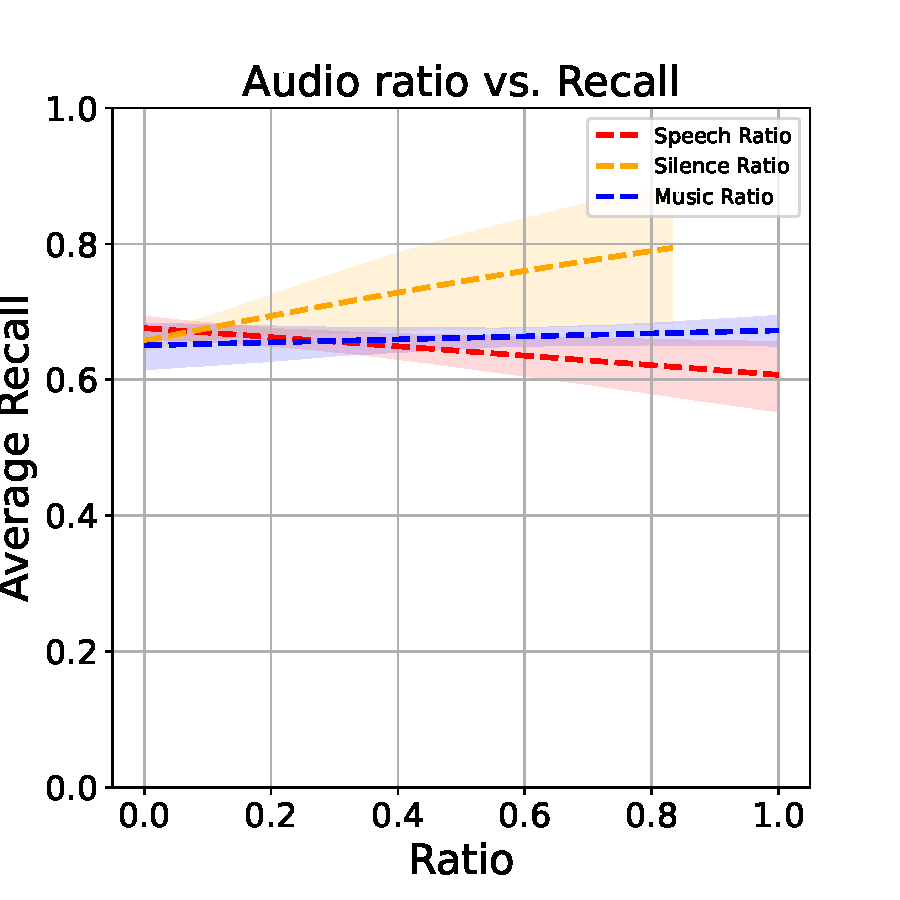
\includegraphics[width=\textwidth]{images/audio1.pdf}
        \caption{}
        \label{subfig:speech vs recall}
    \end{subfigure}
    %\hfill
    \begin{subfigure}{0.3\textwidth}
        \centering
        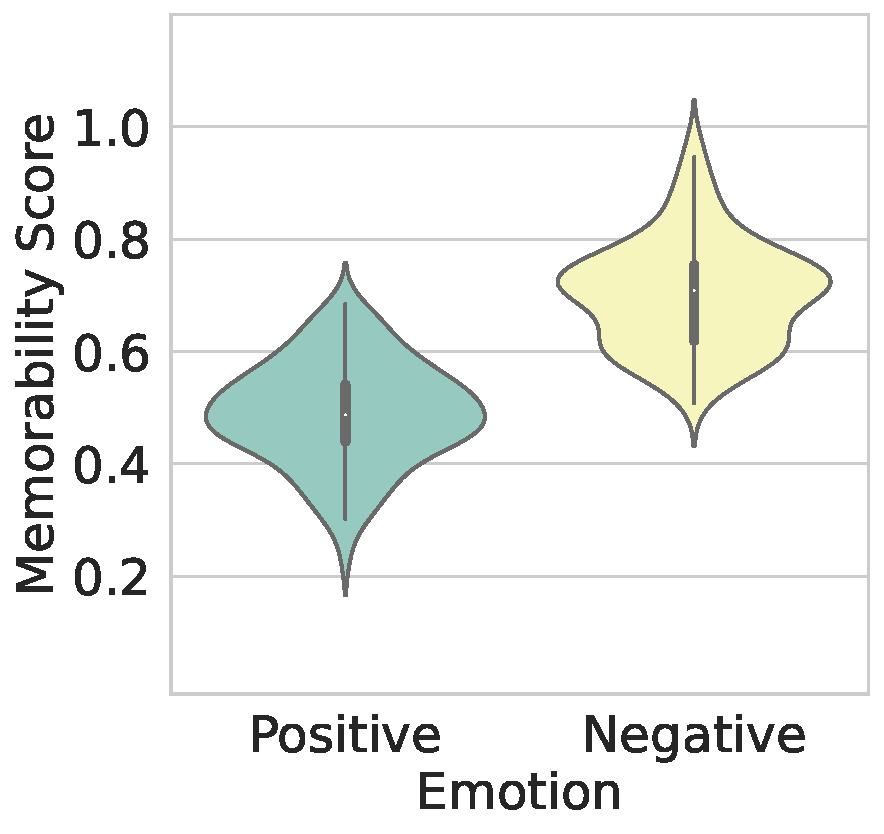
\includegraphics[width=\textwidth]{images/emotion_vs_recall_violin.pdf}
        \caption{}
        \label{subfig:emotion vs recall}
    \end{subfigure}
    %\hfill
    \begin{subfigure}{0.3\textwidth}
        \centering
        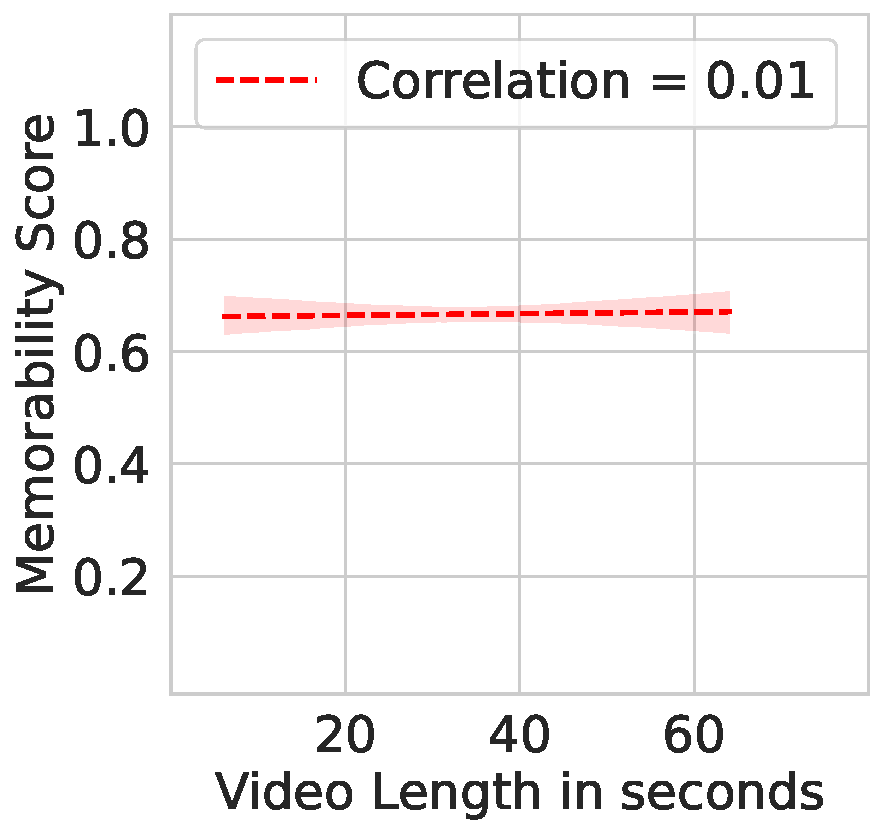
\includegraphics[width=\textwidth]{images/length_vs_mem.pdf}
        \caption{}
        \label{subfig:length vs mem}
    \end{subfigure}
    \begin{subfigure}{0.3\textwidth}
        \centering
        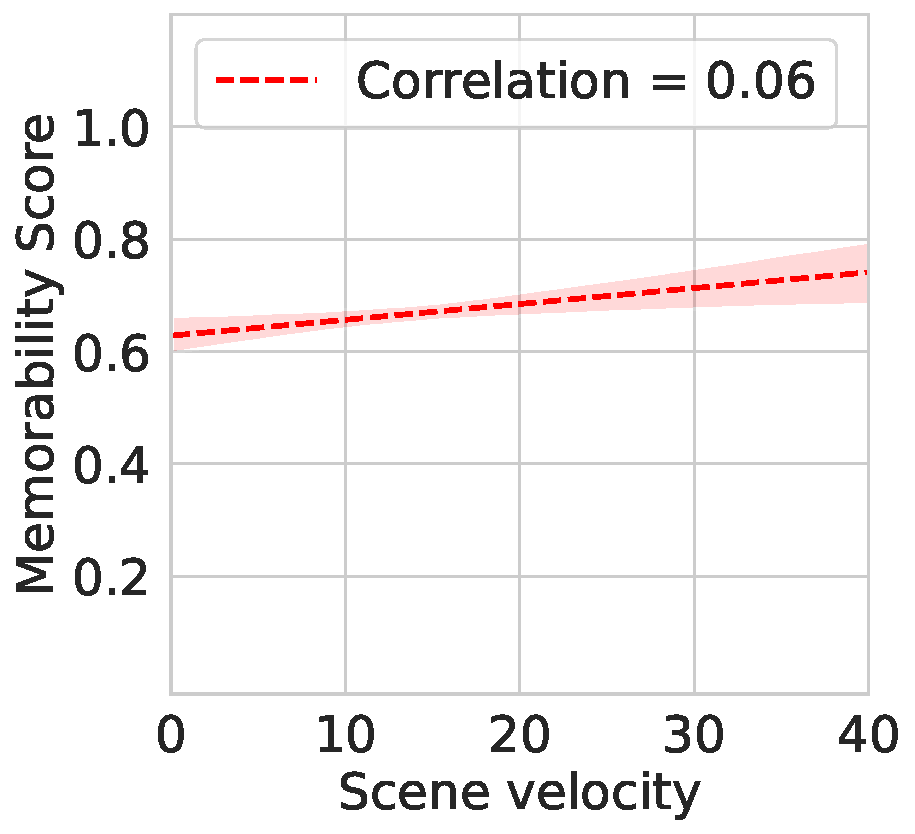
\includegraphics[width=\textwidth]{images/velocity_vs_recall.pdf}
        \caption{}
        \label{subfig:velocity vs recall}
    \end{subfigure}
    \begin{subfigure}{0.3\textwidth}
        \centering
        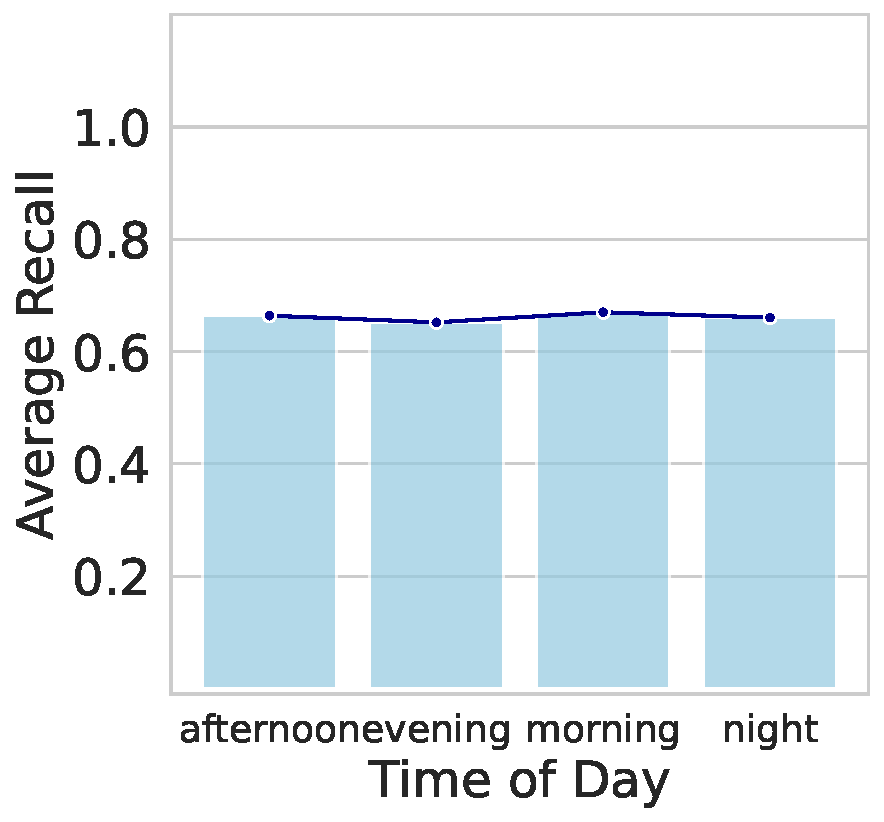
\includegraphics[width=\textwidth]{images/avg_recall_by_time.pdf}
        \caption{}
        \label{subfig:avg recall by time}
    \end{subfigure}
      \begin{subfigure}{0.3\textwidth}
        \centering
        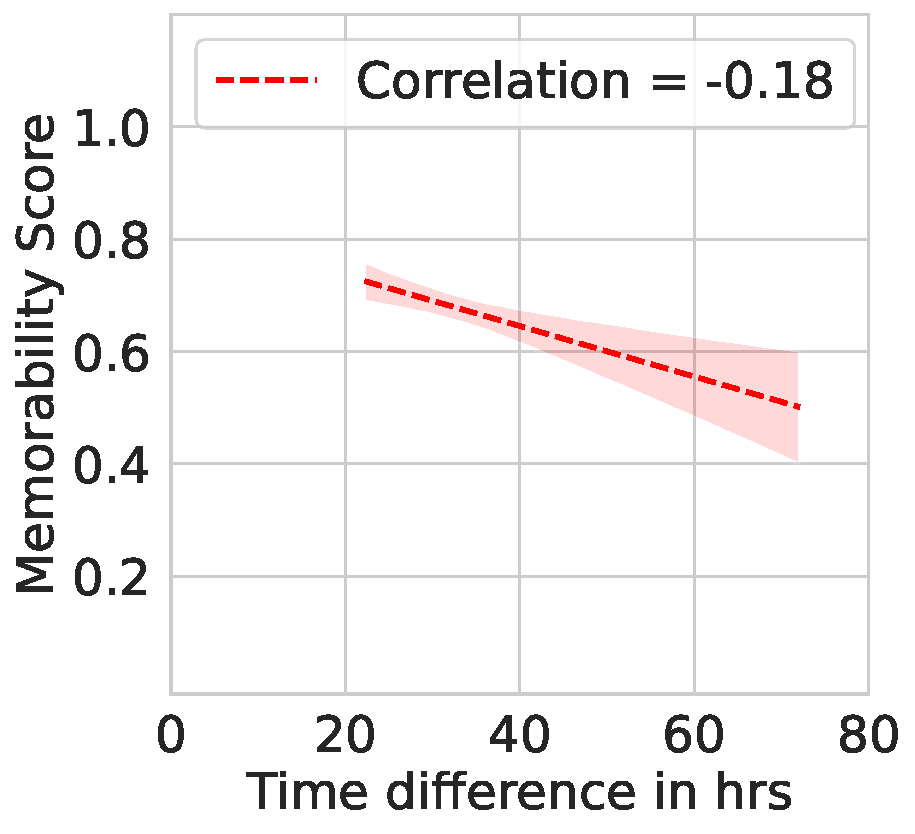
\includegraphics[width=\textwidth]{images/delay_vs_recall.pdf}
        \caption{}
        \label{subfig:delay vs recall}
    \end{subfigure}
    \begin{subfigure}{0.3\textwidth}
        \centering
        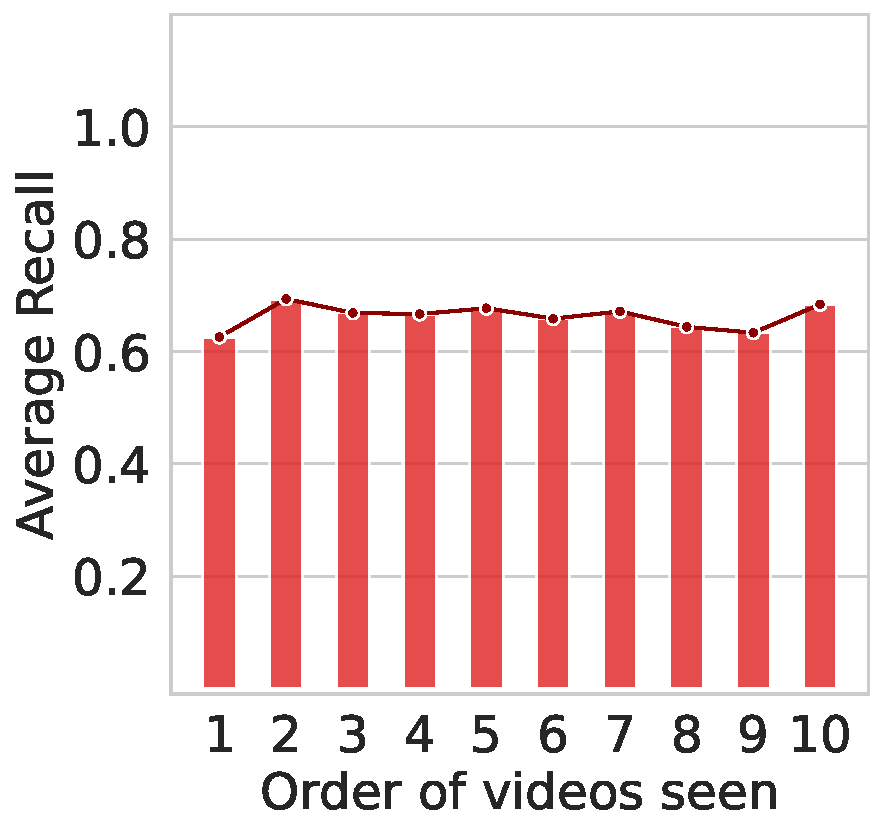
\includegraphics[width=\textwidth]{images/avg_recall_by_position.pdf}
        \caption{}
        \label{subfig:avg recall by position}
    \end{subfigure}
    \begin{subfigure}{0.3\textwidth}
        \centering
        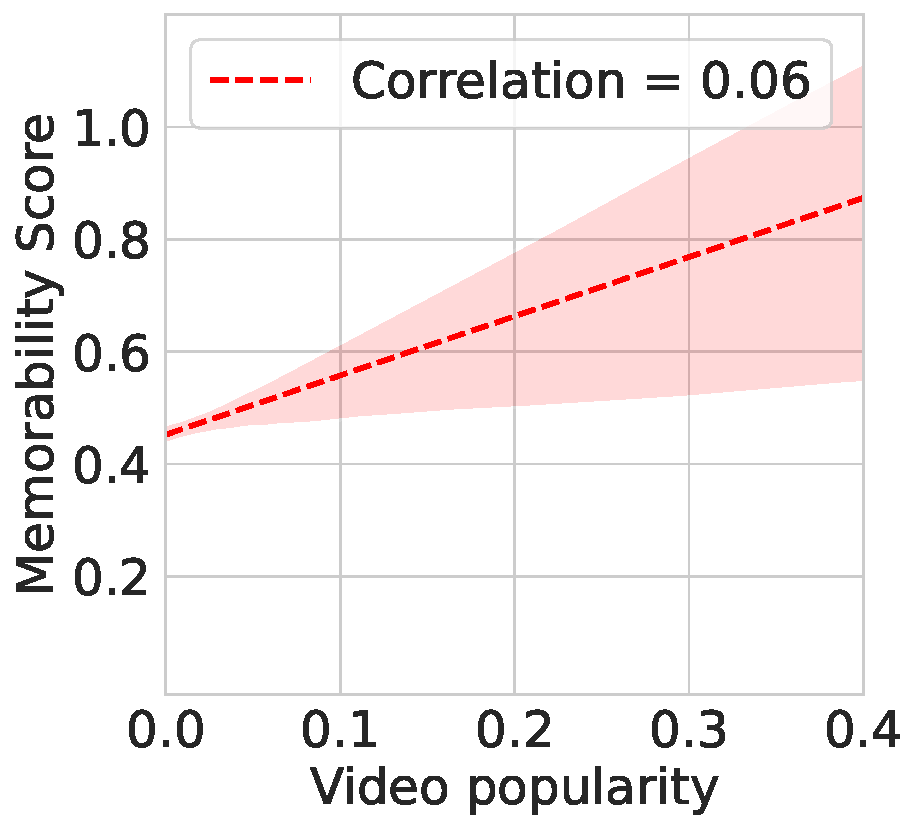
\includegraphics[width=\textwidth]{images/popularity_vs_recall.pdf}
        \caption{}
        \label{subfig:popularity vs recall}
    \end{subfigure}
    \begin{subfigure}{0.3\textwidth}
        \centering
        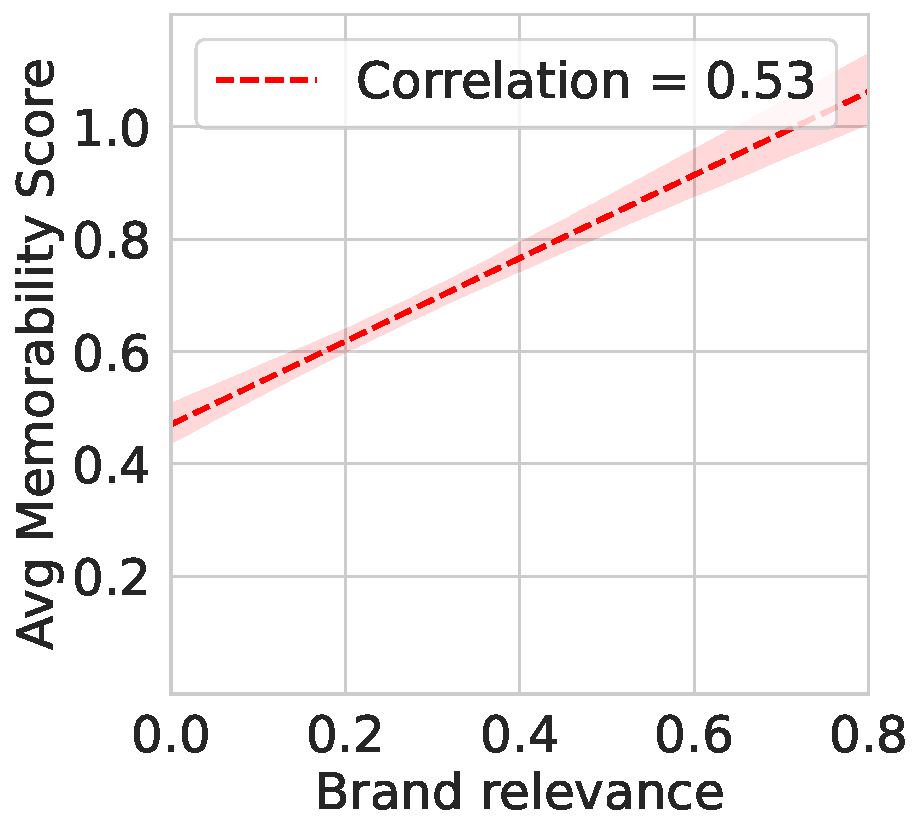
\includegraphics[width=\textwidth]{images/relevance_vs_recall.pdf}
        \caption{}
        \label{subfig:relevance vs recall}
    \end{subfigure}
    \begin{subfigure}{0.3\textwidth}
        \centering
        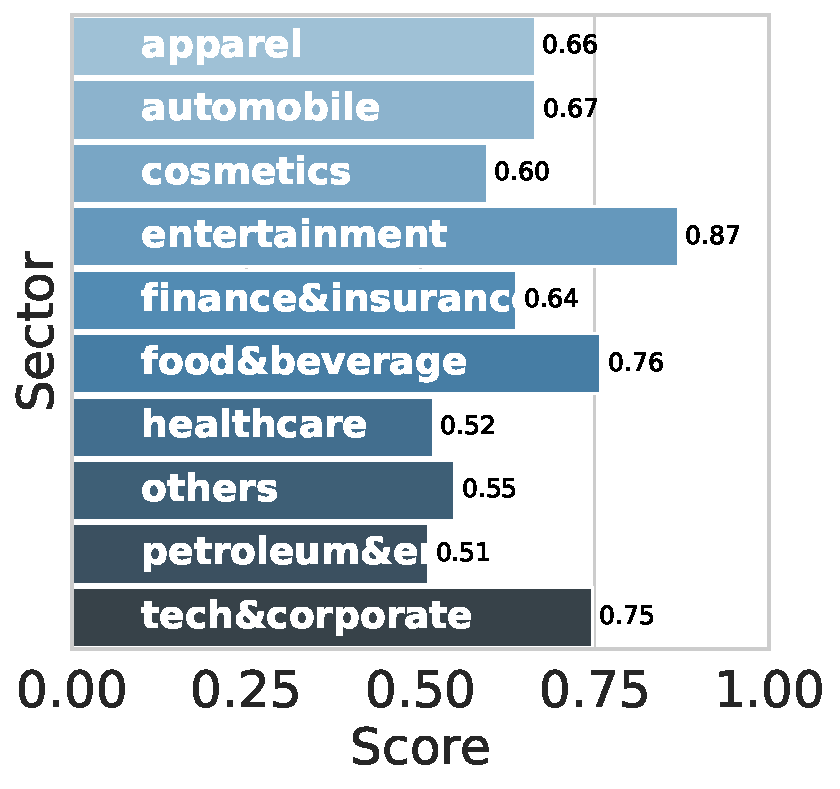
\includegraphics[width=\textwidth]{images/avg_recall_by_sector.pdf}
        \caption{}
        \label{subfig:recall by sector}
    \end{subfigure}
  %\vspace*{-3mm}    
    \caption{Correlations between \textit{content factors} (a-d), \textit{interaction factors} (e-g), and \textit{customer behavior factors} (h-j) with memorability on LAMBDA samples. While emotion has a high correlation with memory, other content factors do not have much correlation. Further, while there is little correlation between the order of videos seen and memorability; with time, participants' memory of the videos shows a forgetting trend. Video popularity, as measured by YouTube likes/views, shows a slight positive correlation with memory. Average brand relevance has a strong positive correlation with memory, with top sectors being remembered as food, entertainment, and tech. Speech, silence and music have little effect with silence having the highest positive correlation with recall. Silence ratio is measured as the percentage of silence in a video, similarly for music and speech.}
    \label{fig:correlation-graphs}
    %\vspace*{-2mm}
\end{figure*}
\end{landscape}










While these studies have contributed much towards understanding the factors that drive customer memory, they are limited in their scope. These field experiments evaluate the effect of a single content factor while controlling for others. Further, these are conducted on a small number of advertisements.% and are unsuitable for training ML models for LTM simulation. %While there have been many works in the ML literature itself to model STM \cite{isola2011makes,cohendet2019videomem}, due to this lack of large-scale datasets for LTM, there have been no works in the ML literature to model LTM. 
%Moreover, from the perspective of psychology as well, there are two stores of memory: short-term (STM) and long-term (LTM). The STM retains a limited amount of content (typically four ``chunks'' of information) in memory for a short period of time (typically less than a few minutes). LTM holds a large amount of content for long periods of time. Content gets transferred from STM to permanently get stored in LTM by processes like repetition, emotional experiences, selective attention, or involuntary processes like consolidation. While there have been many large-scale studies to find out content factors for effective STM storage \cite{isola2011makes,cohendet2019videomem}, there have been no parallel studies for LTM until now.
Therefore, to model LTM over advertisements, we conduct the first large-scale human study on long-term advertisement memorability\footnote{We obtained the Institutional Review Board Approval to conduct the study from our institute.}. We call it LAMBDA (Long-term Ad MemoraBility DAtaset). Over two years, we conducted an LTM study involving 1749 participants across four sessions across two institutes to collect LAMBDA. We collect memorability scores over 2205 ads from 276 brands, covering 113 industries. On day 1, participants saw ads, and after a lag time of at least one day, they answered questions testing their brand recall, ad recall and recognition, scene recall and recognition, and audio recall (\S\ref{sec:Annotation Protocol}). Next, we average the brand recall scores across participants and compute the average long-term ad memorability scores. Then, we use these scores to train machine learning models to predict long-term ad memorability.



 
\textbf{How can we model customer memory?} To model customer memory, we design a novel architecture, Henry\footnote{We name the model Henry in honor of the immense contributions by the patient Henry Molaison (H.M.) \cite{squire2009legacy}. An experimental surgery conducted on him resulted in the discovery of the distinct regions responsible for LTM and STM.} (Fig.~\ref{fig:memorability-model}), incorporating world-knowledge from large language models (Llama \cite{touvron2023llama}), visual knowledge from vision encoder (EVA-CLIP \cite{sun2023eva}) and specialized perception modules covering visual and cognitive knowledge about the ad. The world knowledge helps Henry to understand the semantics of the ad, the brand knowledge and consolidate them with the visual semantics from the ad. The visual encoder helps the model to ``see'' the ad. We convert the visual encoder embeddings to language space using QFormer \cite{li2023blip} and further augment them with specialized ``verbalizations'' involving visual scene descriptors like visual caption, optical character recognition (OCR), automatic speech recognition (ASR), and cognitive descriptors like emotion and scene complexity scores, which help the model ground the visual and cognitive knowledge in the LLM's world knowledge. We train the model on our LTM data samples and obtain higher than human consistency scores. Further, we train Henry on other short and long term image and video memorability datasets in the literature - LaMem, MemCat, SUN, Memento10k, MediaEval, and obtain state-of-the-art performance on all of them. We also show that Henry performs well on unseen datasets in zero-shot settings, performing better than models specifically trained on those datasets.


\textbf{How to generate memorable Ads?}\label{ref:Generation Task} One of the primary goals of modeling content memorability is to generate more memorable content. The task of generating more memorable ads is given the ad description containing the brand and campaign title to generate the ad scenes and dialogues. However, there is no data in the literature for this task. Therefore, we turn to synthetic data generation and LLM-as-a-judge paradigm \cite{khandelwal2023large,zheng2023judging}.
%Drawing inspiration from advancements in reinforcement learning from human feedback (RLHF) research \cite{ouyang2022training,stiennon2020learning}, which addresses the generation of less harmful content, we adopt a two-step process: instruction fine-tuning and preference alignment. To accomplish the generation of memorable ads, 
We first collect a large-scale advertisements dataset, collecting brand name, ad text, time, ad content, and channel. Then, we use Henry as a judge to simulate memorability on the collected ads. We ultimately get a dataset of 5 million advertisements with their automatic speech transcripts, OCR, automatically detected objects, colors, aesthetics, captions, emotions, logos, and memorability scores. We call this dataset UltraLAMBDA. We then select high memorability samples from UltraLAMBDA to train Llama-13B to generate memorable ads. Finetuning LLama for two iterations on this automatically constructed dataset yields an improvement of 44\% in memorable ad generation.

\begin{figure*}[!t]
%\vspace*{-0.2in}
    \centering
    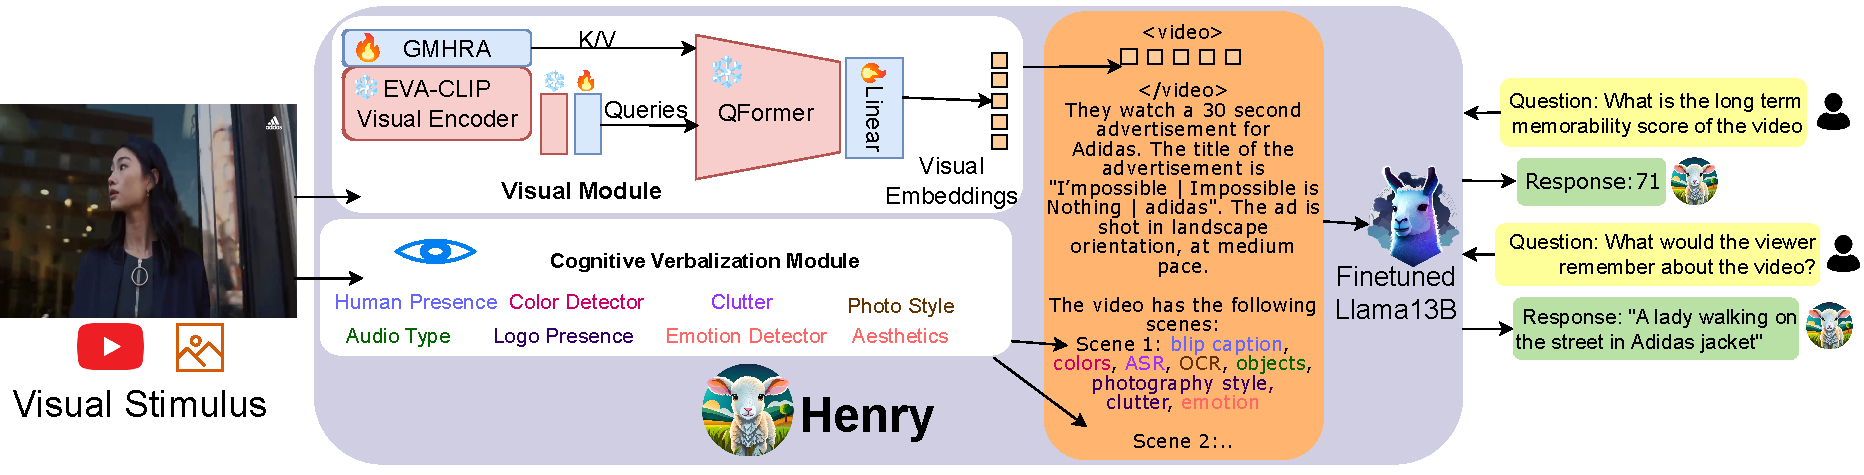
\includegraphics[width=\textwidth]{images/architecture.pdf}
    \caption{Predicting memorability by encoding visual information (via visual encoder EVA-CLIP), cognitive concepts (via verbalization module), and world knowledge (through fine-tuned Llama). We instruction fine-tune the combined model end to end to predict user memorability. Snowflake and fire symbols denote the frozen and unfrozen parts of the architecture.}
    \label{fig:memorability-model}
%\vspace*{-2mm}
\end{figure*}



Our main contributions are summarized as follows:
\begin{itemize}[leftmargin=*]
    \item We release the first large-scale dataset, LAMBDA, on long-term advertisement memorability involving more than 1700 participants. We collect memorability scores over 2205 ads from 276 brands (157/276 brands are from SnP 500), covering 113 industries. Further, we introduce a new protocol to measure customer memory of brands (\S\ref{sec:Annotation Protocol}).
    \item We design a novel model, Henry, which can model both STM and LTM and can incorporate scene understanding, brand knowledge, and speech (\S\ref{sec:Predicting Ad Memorability}). Henry achieves state-of-the-art performance on eight literature image and video memorability datasets (\S\ref{sec:results and discussion}). Further, we show that Henry performs well on unseen datasets in zero-shot settings.
    \item We propose the task of memorable ad generation. We release the first large scale ad dataset, UltraLAMBDA, consisting of 5 million ads with their automatically extracted content labels like ASR, captions, OCR, emotions, and memorability scores assigned by Henry. Using UltraLAMBDA, we first show that large LLMs like GPT-3.5 and 4 are unable to generate memorable content. Then, we train Henry to progressively generate more memorable ads resulting an average improvement of 44\% in memorability scores (\S\ref{sec:Generating Memorable Ads}). Through this, for the first time in literature, we also show the use of synthetic data on a task for which no large scale data exists.
    \item We conduct an extensive set of experiments on memorability prediction, showing the effects of LTM on STM modeling and vice-versa, and the effects of changing world-knowledge with time, scene understanding, brand knowledge, and speech on memorability modeling (\S\ref{sec:results and discussion}).\\
\end{itemize}


%\section{Related Work}

%\textbf{Memory Research In Psychology:} 
%From the perspective of psychology, there are two stores of memory: short-term (STM) and long-term (LTM). The STM retains a limited amount of content (typically four ``chunks'' of information) in memory for a short period of time (typically less than a few minutes). LTM holds a large amount of content for long periods of time. Content gets transferred from STM to permanently get stored in LTM by processes like repetition, emotional experiences, selective attention, or involuntary processes like consolidation. While there have been many large-scale studies to find out content factors for effective STM storage \cite{isola2011makes,cohendet2019videomem}, there have been no parallel studies for LTM until now.

%In order to remember anything, it has to be \textit{encoded}, \textit{stored}, and \textit{retrieved}. \textit{Encoding} is the process of converting incoming information into a form which can be stored or compared with memory contents. \textit{Storage} is the next process where contents are stored in short-term memory (STM) or long-term memory (LTM). The STM retains a limited amount of content (typically four ``chunks'' of information) in memory for a short period of time (typically less than a few minutes). LTM holds a large amount of content for long periods of time. Content gets stored in LTM from STM due to processes like repetition, emotional experiences, selective attention, or involuntary processes like consolidation. Finally, to \textit{remember} stored content, if the content is not in STM, it is brought from LTM to STM and is then served from there. Remembering can be of two types: recall and recognition. Recall is the act of intentionally bringing content from LTM to STM. Recognition is matching an encoded stimulus to incoming stimulus. 








%\vspace{-2mm}
\subsection{LAMBDA Protocol, Study \& Insights}
\label{sec:Long-Term Advertisement Memorability Dataset}
We first give an overview of LAMBDA data collection process and the annotation protocol. We also present some interesting characteristics LAMBDA exhibits about LTM.

\subsubsection{Video Collection}
\label{sec:Video Collection}
In contrast to previous video memorability works where videos were soundless and only of action videos \cite{newman2020multimodal, cohendet2019videomem}, the videos in our dataset come from multimodal ads released on YouTube channels of 276 major brands covering 113 industries%\footnote{Industry information was collected from Wikidata entry of the brand.}
. We collect 2205 such ads spanning over the years 2008-2023. The videos have an average duration of 33 seconds. Out of all the videos, 2175 have audio in them. The collected advertisement videos have a variety of characteristics, including different scene velocities, human presence and animations, visual and audio branding, a variety of emotions, scene complexity, and audio types. 




\subsubsection{Annotation Protocol}
\label{sec:Annotation Protocol}
At the outset, participants are given a preliminary questionnaire aimed at establishing their brand-related interactions and media consumption habits. Participants are given a list of fifteen randomly chosen brand options and are asked to choose those they recall encountering advertisements for during the current year. Subsequently, participants are presented with another set of fifteen brands and are instructed to identify those for which they have personally utilized products within the same timeframe. 

In addition, participants are asked about their utilization of ad-blocking software and their Youtube subscription. The questionnaire further captures participants' digital media habits, including the division of their time spent on YouTube between mobile and web platforms and their preferred channels for acquiring information about new products and brands.

Following the initial questionnaire, participants proceed to the core segment of the study, where they are shown 11 advertisements in a sequential manner. Notably, the eleventh advertisement is deliberately repeated for half of the participants, while it is unique for the other half. To ensure participant engagement, attention-check questions are placed between every two to three advertisements. These questions are common sense questions like ``How many legs does a cow have?''. If the participant fails to answer the question within 10 secs, they are requested to rewatch the video. After the 11th video, participants are asked if they recollect watching the ad in the span of the study. Interestingly, 15\% participants were not able to recognize the repeated video correctly. 



The memorability test involved 1,749 participants: 971 in a take-home setting and 778 in an auditorium. Take-home participants received emailed questionnaires after 24 hours, with responses accepted for 72 hours. Auditorium participants completed questionnaires at 24, 36, or 72 hours, evenly split among these intervals. The questionnaire assessed two types of memory: brand recognition and ad recall. For recognition, participants identified encountered brands from a list of 20 randomly chosen brands. For recall, they described remembered ads for the brands recognized in the previous prompt\footnote{The complete questionnaire for participant one is given in Appendix:\S\ref{sec:Memorability Questionnaire}.}. 

The average memorability score was 67.5\% (SD of 13.6\%). 
To evaluate human consistency, we split our participant pool into two independent halves, and quantified how well memorability on the first half of the participants matched with the second half of the participants. Averaging over 25 random split half trials, we get a Spearman's rank correlation ($\rho$) of 0.77 for brand recall (compared to 0.68 for images in \cite{khosla2015understanding}, 0.616 for videos in \cite{cohendet2019videomem} and 0.73 in \cite{newman2020multimodal}). The estimated D prime for the participants comes out to be 1.848.\footnote{\url{https://en.wikipedia.org/wiki/Sensitivity_index}}


\subsubsection{What makes an Ad memorable?}
\label{sec:What makes an Ad memorable?}
Among the many reasons why an ad might be memorable, we investigate the following factors: \textbf{brand factors} (\textit{viz.,} brand popularity, industry), \textbf{content factors} (\textit{viz.,} video emotion, scene velocity, length, speech to silence ratio), \textbf{customer-content interaction factors} (\textit{viz.,} time of seeing the video, order in which the video was seen, time difference between watching the video and recalling the brand), and \textbf{customer behavior factors} (\textit{viz.,} average relevance of the brand and video popularity).


\begin{landscape}
    \begin{table*}
        \centering
        \resizebox{1.6\textwidth}{!}{%
        \centering \scriptsize
        \begin{tabularx}{1.6\textwidth}{>{\hsize=0.9\hsize}X|>{\hsize=0.3\hsize}X>{\hsize=0.3\hsize}X>{\hsize=0.3\hsize}X>{\hsize=0.3\hsize}X|>{\hsize=0.35\hsize}X>{\hsize=0.3\hsize}X>{\hsize=0.3\hsize}X>{\hsize=0.35\hsize}X}
        \hline
        \multirow{2}{*}{\textbf{Models}} & \multicolumn{4}{c|}{\textbf{Image Datasets}} & \multicolumn{4}{c}{\textbf{Video Datasets}} \\
        & \textbf{Lamem} & \textbf{Memcat} & \textbf{SUN} & \textbf{Merged} & \textbf{Memento10k} & \textbf{VideoMem} & \textbf{MediaEval} & \textbf{\makecell{LAMBDA}} \\
        \hline
        {Human Consistency} & 0.68 & 0.78 & 0.75 & - & 0.73 & 0.61 & - & 0.55 \\
        {10-shot GPT-3.5} & 0.29 & 0.18 & 0.15 & - & 0.07 & 0.06 & 0.06 & 0.06 \\
        {Regression 
        using ViT feats (ViTMem)} & 0.71 & 0.65 & 0.63 & \valgood{0.77} & 0.56 & 0.51 & - & 0.08 \\
        {Current Literature SOTA} & 0.71 & 0.65 & 0.68 & \valgood{0.77} & 0.67 & 0.56 & 0.46 & - \\
        {Henry trained on individual datasets} & \valbest{0.74} & \valbest{0.82}  & \valgood{0.73}  &-  & \valbest{0.75}  & \valbest{0.64}  & \valbest{0.50}  & \valbest{0.55}  \\
        {Henry trained on all (combined) datasets} & \valgood{0.72} & \valgood{0.79} & \valbest{0.76} & \valbest{0.79} & \valgood{0.72} & \valgood{0.60} & \valgood{0.48} & \valgood{0.52} \\
        \hline
        \end{tabularx}%
        }
        \caption{Results of Henry (our model) on eight datasets compared with the current best models reported in the literature and GPT-3.5. Human consistency values are also listed in the top row for reference. It can be observed that our model achieves state-of-the-art performance across all datasets. Best models are denoted in \valbest{green} and runner-ups in \valgood{blue}.
        References for the seven literature SOTA models in the format \{\texttt{dataset: SOTA model citation}\} are: LaMem: \cite{hagen2023image}, MemCat: \cite{hagen2023image}, SUN: \cite{fajtl2018amnet}, Merged Image datasets: \cite{hagen2023image}, Memento10k: \cite{Dumont_2023_CVPR}, VideoMem: \cite{Dumont_2023_CVPR}, MediaEval: \cite{DBLP:conf/mediaeval/LuW21}
        }
        \label{table:memorability-main-results}
    \end{table*}
\end{landscape}




\textbf{Content Factors}: %To answer the question of what is in the content which determines memory, 
Previous studies like \cite{isola2011makes,newman2020multimodal} have investigated the effect of pixel statistics like color and hue, saturation, and value, scene semantics like the number of objects, the area occupied by objects on memorability. In general, low-level semantic features have no correlation with memorability, but higher-level features like the type of scenery has some correlation. For instance, Newman \textit{et al.} \cite{newman2020multimodal} found that videos with
people, faces, hands, man-made spaces, and moving objects are, in general, more memorable than those with outdoor landscapes or dark and cluttered content. Since only our dataset has videos with cognitive features like emotions and are also non-silent, we extend the previous analysis to find the effect of speech and emotion on memory. Fig.~\ref{subfig:speech vs recall} shows the effect of speech. We observe that percentage of speech in a video, presence of music, and type of music have a very little correlation with long term memory. On the other hand, emotions primarily depicted through speech in ads can explain memorability. We see in Fig.~\ref{subfig:emotion vs recall} that negative emotions are more memorable than positive emotions. Further, %in line with other studies \cite{newstead2010cost,varan2020effects}, 
we find that video length has little effect on memorability (Fig.~\ref{subfig:length vs mem}), but scene velocity has a slightly positive correlation with memory (Fig.~\ref{subfig:velocity vs recall}).



\textbf{Interaction Factors:} Memorability may also depend on the time of the day the ad was seen. However, we find that the time of day of watching has almost no effect on the memorability of the ad (Fig.~\ref{subfig:avg recall by time}). It may be expected that memorability decays as time passes. We plot the forgetting curve for ads in Fig.~\ref{subfig:delay vs recall} measuring brand recognition against time elapsed between video viewing and memory assessment. The forgetting coefficient of ads is 0.18, notably than action videos \cite{cohendet2019videomem}. The difference likely arises due to differences in protocols. Cohendet \textit{et al.} (2019) \cite{cohendet2019videomem} used a two-stage memory protocol in which participants did both short-term and long-term recall, thus enhancing their long-term recall. 
Next, we investigate the effect of the order in which the video was watched with its memorability (Fig.~\ref{subfig:avg recall by position}). We see that order of videos seen has little impact on video memorability, with a slight bias in favor of the initial and last ads. %This is in line with other results on ad memorability \cite{terry2005serial}.





%\textbf{Brand Factors}: To understand what kind of brands are remembered more than others, in Fig.~\ref{subfig:recall by sector}, we plot the memory correlations with industry extracted from Wikidata.  This could be explained by the fact that we conducted this experiment on a student population. 


\textbf{Customer Behavior Factors}: It might be possible that the videos which are liked more are remembered more. To investigate this, we test the correlation of popularity as measured by the ratio of Youtube video likes to views with memorability. We see that there is a positive correlation between video popularity and memorability (Fig.~\ref{subfig:popularity vs recall}). Further, in the study, we asked the participants to select the brands they have personally used from a set of 15 randomly chosen brands and similarly choose brands they have seen ads for. To prevent any systematic bias, the brands asked in this question are independent of the brands shown the next day. We plot thus collected brand relevance values with brand recall in Fig.~\ref{subfig:relevance vs recall}. We see that average brand relevance is strongly correlated with average recall (coeff= 0.53), where entertainment, corporate, and food and beverage sectors, which are quite popular brands in a student population are the most remembered, while the others are less remembered (Fig.~\ref{subfig:recall by sector}).


%%%%%%%%%%%%%%%%%%%%%%%%%%%%%%%%%%%%%%%%%%%%%%%%%%%%%%
%%%%%%%%%%%%%%%%%%%%%%%%%%%%%%%%%%%%%%%%%%%%%%%%%%%%%%
%\vspace{-2mm}
\subsection{Predicting Ad Memorability}
\label{sec:Predicting Ad Memorability}


In this section, we focus on predicting memorability - both long-term and short-term for both videos and images. We pose memorability prediction as a problem that needs (a)~\textit{visual knowledge} to identify and understand visual concepts across images and videos like shapes, colors, objects, and scenes, (b)~\textit{cognitive knowledge} relevant to marketing, for example, ad emotions, scene complexity, scene aesthetics, and (c)~\textit{world knowledge} to relate the captured visual and marketing concepts to real-world concepts capturing their function, use, and interaction patterns. %Recently, models like BLIP \cite{li2023blip}, Llava \cite{liu2023visual}, and Video4096 \cite{bhattacharya2023video} have shown that visual signals can be successfully mapped to language semantics, allowing us to leverage visual knowledge from visual embedding models like ViT \cite{dosovitskiy2020image} and world knowledge from LLMs. 
For instance, when Airbnb\footnote{See Fig.~\ref{fig:airbnb-ad}) for the ad} shows an adult female and a male with the text, ``Our guest room is paying for our wedding''; it denotes a couple saying that renting out their space on Airbnb helps them sponsor their wedding \cite{kumar2023persuasion}. World knowledge captured in LLMs, together with the visual knowledge of ViT and marketing knowledge through specialized cognitive models, helps to (i)~identify the two adults as a couple, (ii)~AirBnb as a housing company, (iii)~recognize the warm emotional tone of the text, and make sense of all three concepts together. Fig.~\ref{fig:memorability-model} shows the proposed architecture of Henry. %The overall process involves passing visual content in the form of video or image through a visual embedder, which maps the visual content into a language space with the help of QFormer \cite{li2023blip}. We find that describing the visual content in language and combining it with the video/image tokens helps for better prediction. The resulting content tokens, along with experiment descriptions, are fed into the Henry to predict memorability scores between 00 to 99. We discuss each part of the architecture and training next.







\begin{landscape}
    \begin{figure*}
%\vspace*{-0.2in}
    \centering
    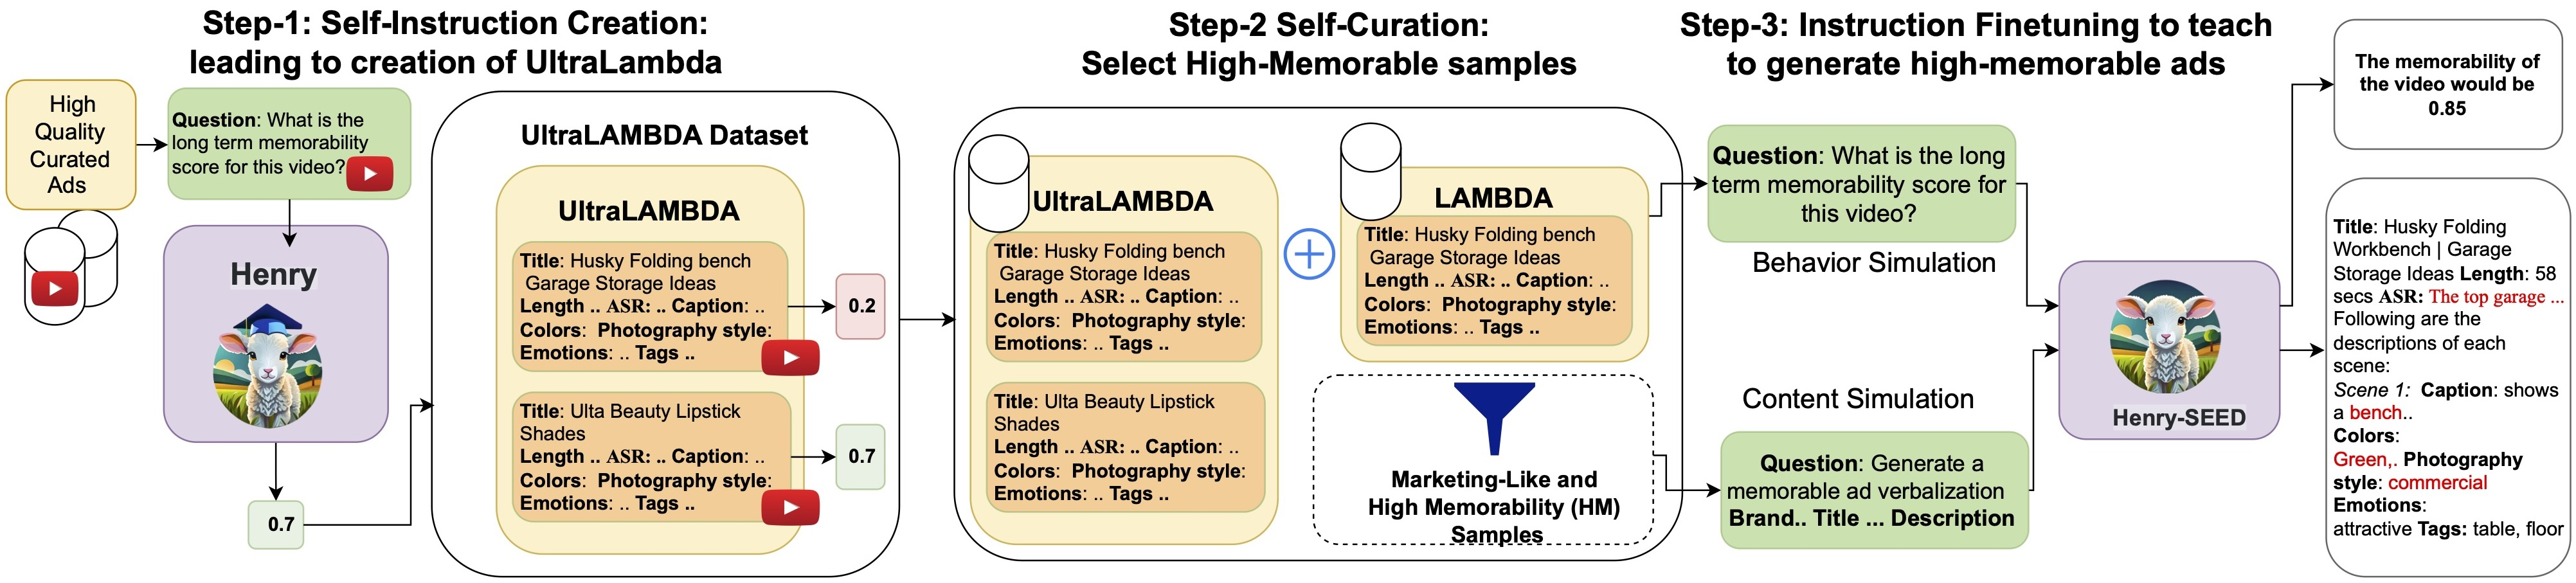
\includegraphics[width=1.6\textwidth]{images/seed-2.jpg}
    \caption{Overview of our SEED method for memorable ad generation. Our self-alignment consists of three steps: (i)~\textbf{Self-instruction creation}: We first collect 5 million high-quality ads from YouTube, Facebook, and other mediums. Henry (trained on the complete train+test sets of LAMBDA) is then used to rate this curated set in an LLM-as-a-Judge fashion. (ii)~\textbf{Self-curation}: We select marketing-like and high-memorability samples from the UltraLAMBDA and LAMBDA datasets. (iii)~Instruction fine-tuning: Henry-SEED is trained on the self-curated set using two tasks: Behavior Simulation and Content Simulation. 
    %\vspace*{-2mm}
    \label{fig:Henry-SEED}}    
\end{figure*}
\end{landscape}


\iffalse
**Give the p-values for each of these as well.**
Following graphs:
1. Mem vs popularity as measured by likes/subscriber count
2. Mem vs emotions
3. Mem vs scene velocity?
4.. Mem vs Industry
5. Mem vs relevance
6. Mem vs time between watch and QA
7. Mem vs time of seeing
8. Mem vs order of video
9. Mem vs length
10. mem vs speech ratio




Images:

1. Least memorable & most memorable videos collage
2. least & most memorable brands collage
3. Study protocol in appendix



Metrics:
1. Average and std deviation of all memorability scores
2. Repeat detection accuracy
3. 


Variables for the video study:
  1. Video
  2. User responses:
      a. Brand Recall
      b. User comments about the video
  3. Video features:
      a. Title
      b. Description
      c. ASR
      d. OCR
      e. Scene recognition
      f. Length



The average memorability score was 67.5\% (SD of 13.6\%). 
To evaluate human consistency, we split our participant pool into two independent halves, and quantified how well image scores measured on the first half of the participants matched image scores measured on the second half of the participants.Averaging over 25 random split half trials, we calculated a Spearman's rank correlation (ρ) of 0.83 between these two sets of scores. 

Verbalization Formats:
Video + Video Features + User responses + Aggregate User features

\fi






\subsubsection{Encoding Multimodal Content}
\label{sec:Encoding Visual Content}
The primary goal of this step is to effectively leverage the ``world-knowledge'' capabilities of the pre-trained LLM. We choose Llama \cite{touvron2023llama} as our base LLM. We employ two techniques to convert visual data into language: encoding visual frames into the LLM space and verbalizing cognitive concepts into language space. We detail the two steps next.

\textbf{Sampling Frames:} %To handle videos, we sample their most important frames. %We explore three different video sampling techniques: uniform sampling, intensity based scene change sampling, and cinematographic sampling. In uniform sampling, frames are sampled at a fixed rate. Since scene duration in advertisements has a very high variance (fast single shots to show action and adventure and slow shots used for telling a story), choosing a uniform threshold leads to a lot of duplicate frames for slower ads or frames getting skipped for faster ads. In the intensity based scene change sampling approach, scene changes in the video are detected by measuring the change in RGB intensity and cosine similarity from VGG across consecutive frames \cite. This gives reasonably better scene changes. However, in the RGB space, visually dissimilar scenes are still not detected, \textit{e.g.} Red and Orange scenes \cite{XYX}. To select a dominant frame in a scene, we select the frame with the highest pixel velocity \cite{XYX}. 
%Finally, 
We detect scene changes by analyzing changes in HSV intensity and edges in the scene, with a 0.3 threshold. We choose the threshold value from the 30-degree rule inspired by the concept of jump-cut avoidance in cinematography \cite{arev2014automatic,friedman2004knowledge}. The 30-degree rule can be formulated as follows: after a ``cut'' (camera stops and re-starts shooting), the camera angle must change by at least 30 degrees.
For dominant frame selection common blur/sharpness heuristics fail in presence of text in image. So we extract the frame with the least changes using \cite{xu2022gmflow}.



\textbf{Encoding Into Language Embedding Space:} To give visual knowledge to Henry, we use EVA-CLIP visual embedder \cite{sun2023eva}. We find that Global Multi-Head Relation Aggregator (GMHRA) \cite{li2021uniformer} helps aggregate the ViT's information better across the time dimension. Next, to effectively leverage the LLM's rich language representations, we use a pretrained Q-Former from BLIP-2 \cite{li2023blip} with an extra linear layer and additional query tokens to convert from visual tokens to language tokens.






\textbf{Verbalizing Cognitive, Experimental, Visual Concepts}
\label{sec:Verbalizing Visual Content}
While visual content encodings are a good representation of the visual characteristics of the image, we find that they are still unable to capture rich cognitive and semantic information present in images. Therefore, to augment the cognitive understanding of the LLM, we verbalize the frame semantic information using the set of features that came out important in our memorability analysis (Fig.~\ref{fig:correlation-graphs}) \cite{bhattacharya2023video,singh2024llava}. The cognitive and visual features are given in Table~\ref{table:scene-verbalization-format} and Listing~\ref{listing:memorability-prediction-verbalization-format}. We find that our cognitive verbalization helps ground the visual perception of LLM in the marketing concepts of the image, helping in downstream prediction performance (Table~\ref{table:architecture-ablation}). %For videos, we use the following additional information: YouTube provided title and description, video duration, and brand information. We pass the video story, described by the concatenation of scene descriptions similar to images, along with their corresponding timestamps and flow based scene velocity to the LLM.





%\vspace{-2mm}
%\subsection{Verbalizing Experiment Conditions} 
%\label{sec:Verbalizing Experiment Conditions}
%We find that verbalizing experimental conditions help give context to the LLM about the task. Details like task type (long-term, short-term), data distribution (for eg: video advertisements, images of natural scenes), subject descriptions (for eg: college students from X college) are given to the LLM. For example, the subjects are students from MIT, and they are shown images of faces and their short term memorability is recorded. We find that this also helps us in solving another challenge: a few samples in datasets like Lamem and Memcat are repeated, but since the experiments were conducted in different settings, the model gets confused if we don't explain the experimental context.

%\vspace{-2mm}
\subsection{Two-Stage Training}
\label{sec:Two-Stage Training}
%Following prior works like \cite{liu2023visual,li2023videochat,li2023blip,zhu2023minigpt,ge2023planting,zhang2023video}, 
We do two-stage training where in the first stage, we utilize the Webvid \cite{bain2021frozen}, COCO caption \cite{chen2015microsoft}, Visual Genome \cite{krishna2017visual}, CC3M \cite{sharma2018conceptual}, and CC12M \cite{changpinyo2021conceptual} datasets to align the visual encoder embeddings with LLM via a large-scale pretraining approach. In the second stage, we train the model with high-quality memorability instructions prepared by following the approach described in the last paragraphs. Henry takes the concatenated inputs, representing the contextual information, and is trained to predict the memorability score of the given image or video within the range of 00 to 99 (see Listing~\ref{listing:memorability-prediction-verbalization-format}). The memorability score of a video, is the percentage of times the participants recall the video correctly (we normalise it to an integer value between 00 and 99 to facilitate the LLM training). During training, the LLM predicts from the complete vocabulary, while during inference, we use the softmax function over numeric tokens only to obtain a number.




\subsubsection{Results and Discussion}
\label{sec:results and discussion}
We conduct extensive experiments on all literature datasets, covering both videos and images, STM and LTM. We compare Henry\footnote{Computing infrastructure used to conduct the experiments along with hyperparameters are given in Appendix:\S\ref{sec:experimental-details}. All experiments are conducted with three random seeds and averages are reported.} with the current state-of-the-art models in the literature across eight datasets, including 10-shot GPT-3.5 (text-davinci-003) \cite{ouyang2022training} where we provide GPT with the same verbalization (for 10 examples), as we provided to Henry, as well as with prior regression based methods using features extracted from ViT L-14 \cite{hagen2023image}. Results are shown in Table~\ref{table:memorability-main-results}, which demonstrate that Henry outperforms all the seven models in the literature across all the seven datasets.



\begin{comment}
    59.43\% - Henry vs Original
    61.36\% - Henry vs GPT-4
    38.63\% - GPT4 vs Henry
\end{comment}





We also conduct extensive ablations to understand the effect of different kinds of data and architectural choices. Tables~\ref{table:memorability-main-results} and Table~\ref{table:data-ablation} show the data ablations. We see that combining datasets actually worsens the performance across all the datasets except the SUN dataset. Further, we find that in zero-shot settings, STM helps in predicting LTM relatively much better than vice versa. This corroborates with the studies in psychology which show that for a content to get committed to LTM, it has to pass through STM \cite{norris2017short}. Therefore, content memorable, according to STM, has an effect on LTM but, interestingly, not vice versa. %We find that if the model is trained on videos, it generalizes well for images as well. The same fact remains true when the model is trained for images and tested on videos except for our dataset. The image memory models generalizing for videos has also been observed by \citet{newman2020multimodal,cohendet2019videomem}. However, this does not scale to our dataset. We posit this might be due to the nature of the prior datasets, which contain videos with just actions while our content is more semantic. 
Further, we observe that Henry loses performance for unseen brands. This underscores the importance of scaling the study across more brands. Next, we evaluate the impact of various architectural choices  (Table~\ref{table:architecture-ablation}). We find that Henry's vision branch is not strong enough by itself to produce good results. Cognitive features that were found important in our study also improve prediction performance. Low-level features like objects and colors have the maximum impact on STM, but higher-level features like emotion, ASR, and aesthetics have a higher impact on LTM.
%We find that the choice of GMHRA for global aggregation of visual features and Qformer to convert visual tokens to language tokens results in improvements across all datasets. Further, interestingly, we observe that despite the task being a computer vision task, the vision tokenization branch of the network contributes less than the language and verbalization branches of the network. However, finally combining both the branches together results in the best performance across all the datasets.


%%%%%%%%%%%%%%%%%%%%%%%%%%%%%%%%%%%%%%%%%%%%
%%%%%%%%%%%%%%%%%%%%%%%%%%%%%%%%%%%%%%%%%%%%
\subsection{Generating Memorable Ads}
\label{sec:Generating Memorable Ads}






We introduce the new task of memorable ad generation. Given inputs like a brand name, a brief campaign description, and the desired ad duration, the goal is to generate a memorable ad featuring scene descriptions, characters, and dialogues. While most memorability research focuses on assessing how memorable content is, little attention has been given to generating memorable content \cite{danescu-niculescu-mizil-etal-2012-hello,khosla2013modifying,siarohin2017make,goetschalckx2019ganalyze,kyle2022modulating}. This gap exists primarily due to the lack of a sufficiently large dataset for training models to generate memorable ads. To address this, we release a large-scale dataset of raw ads and propose the Self-rEwarding mEmorability moDeling (SEED) method, which leverages raw ads to create memorable ones.

\textbf{SEED method} (Fig.~\ref{fig:Henry-SEED}):  \textit{Step 1: Self-Instruction Creation:} We gather a dataset of 5 million raw ads sourced from social media platforms, including Facebook, Twitter, Snapchat, and YouTube. For each ad, we collect the brand name, ad title, links, captions, dates, and ad assets (videos and images).


\textit{Step 2: Self-Curation:} Since these ads are publicly sourced, we employ few-shot Mistral-7B \cite{jiang2023mistral} to clean and filter the ads, ensuring they are marketing-focused, semantically relevant, and use proper language (Listing~\ref{listing:Mistral Prompt for Ad Filtering}). We then automatically label the ads with cognitive features critical for modeling memorability (Table~\ref{table:scene-verbalization-format}). %Leveraging  synthetic labels from expert LLMs \cite{zhou2023customization,li2023self,khandelwal2023large,zheng2023judging}, 
Subsequently, we use Henry to label the ads for memorability scores. This results in a dataset we call \textit{UltraLAMBDA}, from which we select high-memorability ads with scores above 65.


\textit{Step 3: Instruction Fine-Tuning:} We then train LLaMA-13B to perform two tasks simultaneously: behavior simulation (predicting ad memorability based on ad content; Listing~\ref{listing:memorability-prediction-verbalization-format}) and content simulation (generating ad scenes and dialogues from a brand name, ad title, and required duration; Listing~\ref{listing:advertisement-generation-prompt-Henry-SEED}). We refer to the model trained using the SEED process as Henry-SEED (Fig.~\ref{fig:Henry-SEED}).


\subsubsection{Evaluation} 
We assess the generated ads using four key metrics: (1)~memorability, as determined by Henry-Oracle\footnote{The Henry model trained on the complete (test+train sets) LAMBDA.}, (2)~memorability evaluated using perplexity of the generative models on ground-truth high/medium/low ads, (3)~ad quality as judged by GPT-4, and (4)~ad quality as evaluated by humans. Although content memorability is assessed by average human recall, it is important to note that humans cannot accurately predict how memorable content will be for others \cite{isola2013makes}. A true test of memorability for generated ads would require a memorability study akin to LAMBDA, which is costly and unscalable due to the number of models and generated ads. Therefore, we measure the memorability of generated ads using two approaches: Henry-Oracle and perplexity on ground truth memorable ads in LAMDA. 

In evaluation using \textit{Henry-Oracle}, the expectation is that the generated ad's memorability should be at par with high-memorable samples (score$>$65) and better than the low (score$<$44) and medium memorability samples (44$<$score$<$65). Perplexity on ground truth low and high memorable ads evaluates the generative model's propensity to generate more memorable content. A stronger model should have a lower perplexity on more memorable content than less memorable content (refer \S\ref{sec:Perplexity evaluation} for details on perplexity evaluation). 



\begin{landscape}
    \begin{table*}[]
    %\vspace*{-0.2in}
    \centering
    \resizebox{1.58\textwidth}{!}{%
    \begin{tabular}{lllllllll|lll}
    \hline
    \textbf{Model} & \textbf{\# Params} & \textbf{Training} & \textbf{Dataset} & \makecell{\textbf{High Quality}\\\textbf{Mem Samples}} & \multicolumn{4}{c}{\textbf{$\Delta$ Memorability}} & \multicolumn{3}{c}{\textbf{Ad-Quality}} \\
    && & & & \makecell{Low} & \makecell{Med} & \makecell{High} & Avg & \makecell{GPT-4\\Consistency} & \makecell{GPT-4\\Preference} & \makecell{Human-\\Preference}\\\hline
    GPT-4 5-shot &$>$175B & ICL & $LAMBDA_{High}$ & 5 & +48 & \valgood{+18} & -13 & +17.6& \valbest{7.73}  & \valbest{91.3\%}  & \valgood{41.8\%}\\
    GPT-3.5 5-shot&175B & ICL & $LAMBDA_{High}$ & 5 & +35 & +5 & -31 & +3 & 7.17 & 84.2\% & - \\
    GPT-3.5 3-shot&175B & ICL & $LAMBDA_{High}$ & 3 & +34 & +6 & -32 & +2.6 & 6.98  & 83.1\% & - \\
    Henry-SEED &13B& SEED & $UltraLAMBDA$ & 800k & +41 & \valgood{+18} & +1 & +20 & 7.34 & 74.7\% &   -\\
    \midrule
    Henry-SEED & 13B& SEED & $UltraLAMBDA$ + $LAMBDA_{High}$ & 820k & \valbest{+89} & \valbest{+31} & \valbest{+12} & \valbest{+44} & \valgood{7.44} & \valgood{85.6\%} & \valbest{60.48\%}\\
    Henry-SEED & 13B&SEED & $LAMBDA_{High}$ & 650 & +78 & +13 & \valgood{+1} &  \valgood{+30.6} & 5.03 & 63.9\% & - \\
    Henry-SEED & 13B&SEED & $UltraLAMBDA$ & 50k & +12 & +9 & -6 & +5 & 6.01 & 66.1\% & - \\
    Henry-SEED & 13B& SEED & $UltraLAMBDA$ (w/o high-mem filtering) & 2M & +19 & +5 & -45 & -7 & 6.73  & 71.1\% & - \\\hline
    \end{tabular}}
    \caption{\textbf{Ad Generation}: Results of Henry-SEED compared with in-context-learning (ICL) GPT-3.5, 4 on Ad-Memorability and Ad generation quality. See \S\ref{sec:Generating Memorable Ads} for details of the metrics computed. We see that Henry-SEED generated ads are more memorable than ads generated using 15x larger GPT-3.5 and GPT-4. We test ad quality using GPT-4 as judge and then test the top-two models using human annotators. GPT-4 as a judge rates GPT-4 and Henry-SEED as the top two models. Subsequently, we ask humans to select between the original and generated ad stories. We observed that human annotators preferred Henry-SEED ads more than the original ads 3/5 times, while GPT-4 generated ads are preferred 2/5 times over the original ads. Further, we note that an increase in the amount of training data for Henry-SEED increases its performance across all metrics. Figs.~\ref{fig:brainly-generated-ad}-\ref{fig:maytag-generated-ad} and Listings~\ref{lst:maytag}-\ref{lst:publix} contain some qualitative samples generated using Henry-SEED. \label{tab:Henry-SEED-generating-memorable-ads}}
    %\vspace*{-3mm}
    \end{table*}
\end{landscape}








%First, to teach Henry to generate ads given the brand name and marketing brief, we finetune it on the UltraLAMBDA samples (Fig.~\ref{fig:Henry for memorable ad generation}). We define two dataset splits for this task Supervised-Fine-Tuning (SFT): fine-tuning on all (potentially noisy) samples of UltraLambda, Preference-Fine-Tuning (PFT): SFT combined with oversampling of (cleaner) most memorable ads from LAMBDA. Since we only generate the verbalization, not the actual video rendition, we consider offline learning RLHF algorithm, ILQL \cite{snell2022offline}. We compare generations of PFT, SFT, PFT+RLHF, and SFT+RLHF models with in-context-learning based Henry, GPT-3.5, 4 generated ads. \cy{Not clear what model you used for finetuning..}






\begin{comment}
    \begin{table}[!t]
    \vspace{-5mm}
    \centering
    \resizebox{0.45\textwidth}{!}{%
    \begin{tabular}{lllll}
    \hline
    \textbf{Model} & \textbf{Training} & \multicolumn{2}{c}{\textbf{Memorability Reward}} & \makecell{\textbf{Preference}}\\
    & & \makecell{LM} & \makecell{HM} & \\ \hline
    GPT 3.5 & 5-shot   & 0.38 & 0.82 & -          \\
    GPT 4 & 5-shot   & 0.39 & 0.81 & -          \\
    GPT 3.5 & 3-shot   & 0.34 & 0.75 & -          \\
    Henry & 3-shot   & 0.29 & 0.62 & 12\%       \\ \hline
    Henry & SFT      & 0.34 & 0.6  & \valgood{41\%}       \\
    Henry & PFT      & 0.40 & 0.77 & 34\%       \\
    Henry & SFT+RLHF & \valgood{0.48} & 0.83 & 39\%       \\
    Henry & PFT+RLHF & \valbest{0.54} & \valgood{0.88} & 35\%\\\hline
    Test Data & - & 0.41 & \valbest{0.89} & \valbest{84\%}\\ \hline
    \end{tabular}
    }
    \caption{Results of Henry compared with in-context-learning GPT-3.5, 4 on Memorability Reward and Preference. Memorability reward is computed on ground-truth LAMBDA samples (LM = samples with memorability $<0.75$, HM = samples with memorability $>0.75$). Preference denotes how much \% times GPT-3.5 prefers the generated scenes and dialogues. Henry is able to improve memorability on LM samples by 25\%. Interestingly, the content generated by GPT-3.5 and 4 has low memorability.}
    \vspace{-3mm}
    \end{table}
\end{comment}


\begin{figure}[]
    \centering
    \includegraphics[width=\textwidth]{images/henry/Henry-Brainly.drawio_compressed.pdf}
    \caption{Henry-SEED Prompt: \textit{Generate the detailed description of a 30-second memorable advertisement titled "Brainly Keep Learning 30sec Final 16x9" for the brand Brainly}. Link to the original ad: \url{https://www.youtube.com/watch?v=kytRXyWXivU} Original Memorability score: 85. Memorability score of Generated Ad: 99.}
    \label{fig:brainly-generated-ad}

\end{figure}






\begin{comment}\somesh{I think we should specify that we use a language only LLM here, because visual tokens for generated ads are unavailable right now. I trained one more epoch the same model removing the image from the MLLM. The performance drop is 10.3\% (0.58 -> 0.52)}\end{comment}


Using \textit{GPT-4 as judge}, we test two ad-quality metrics: \textit{consistency} and \textit{preference}. 
Consistency assesses how coherent the generated story is—both internally (e.g., between dialogues) and in relation to the provided brand information and title (Listing~\ref{lst:ad-quality-consistency-prompt}). 
Preference measures how often GPT-4 favors the generated story over the original (Listing~\ref{lst:ad-quality-preference-prompt}). In \textit{human evaluation}, we ask human annotators to select between the generated and the original ad stories without revealing which is which (\S\ref{sec:Questionnaire to Gather Human Preferences over Generated Ads}). This evaluation is conducted with 20 non-expert annotators and 3 ad industry experts with over 5 years of experience in the creative industry. The expectation is that the quality of synthetic ads should be comparable to that of the original ads.

%To generate ads, the brand names and titles are sourced from the test split of the LAMBDA dataset, and then models like GPT-4 and Henry-SEED are asked to generate ads given the brand and title. Then the generated ads are evaluated using Henry-Oracle, Perplexity, GPT-4, and humans. 












\subsubsection{Results}  
We compare the following models to generate memorable ads: LLaVA model trained on UltraLAMBDA (we refer to this model as Henry-SEED), GPT-3.5, and GPT-4. GPT-3.5 and 4 are LLMs with strong generative capabilities with high performance across many benchmarks \cite{brown2020language}. 


\textbf{Evaluation of memorability of the generated ads:} 
Table~\ref{tab:Henry-SEED-generating-memorable-ads} compares models based on the average increase in memorability, as evaluated by the Oracle model trained on both the train and test sets. Table~\ref{table:perplexity-scores-ultralamda} shows the perplexity of LLaVA before and after training on UltraLAMBDA. Notably, Henry-SEED, trained on UltraLAMBDA, significantly improves memorability scores across all bins (Low, Medium, and High). Although GPT-4 and GPT-3.5—despite being 15x larger—improve the memorability of ads with initially low ratings, they decrease the memorability of ads with high ratings. Table~\ref{table:perplexity-scores-ultralamda} further contrasts untrained and SEED-trained LLaVA, revealing that the SEED method greatly reduces perplexity on high-memorability samples. While LLaVA originally had higher perplexity for high-memorable samples, training on UltraLAMBDA shifts this trend: perplexity increases for low-memorability samples and decreases for high-memorability ones. This suggests the SEED approach enhances the likelihood of generating high-memorable ads while reducing the likelihood of producing low-memorable ones.


Importantly, UltraLAMBDA contains no overlap with LAMBDA. Neither Henry (used to label memorability for UltraLAMBDA) nor Henry-SEED (trained on UltraLAMBDA) was trained on LAMBDA’s test-set ads. Despite this, Henry-SEED demonstrates significant improvement in performance compared to GPT-3.5 and GPT-4.


\textbf{Evaluation of the quality of the generated ads:}
When comparing ad quality, we find that while GPT-4 favors its own generated ads 91.3\% of the time, Henry-SEED follows closely with an 85.6\% preference score. In human evaluations, where annotators were asked to choose between original and generated ads based on quality, Henry-SEED's ads were preferred around 60\% of the time—approximately 20\% more than GPT-4's ads.


\textbf{Qualitative Results:} Figs.~\ref{fig:brainly-generated-ad}-\ref{fig:maytag-generated-ad} and Listings~\ref{lst:maytag}-\ref{lst:publix} show some randomly sampled ad storyboards generated by Henry-SEED and Sec.~\ref{sec:Expert Feedback Collected For Generated Ads} contains some expert comments over the generated ad storyboards. These qualitative examples are generated by prompting Adobe Firefly \cite{adobefirefly} with the scene descriptions provided by Henry-SEED\footnote{Note: We do not make any changes to Henry-SEED's generation for the voice-over or the scene descriptions before passing it to Firefly.}, followed by pasting OCR from the Henry-SEED generated verbalization on top of the generated images. %Finally, we segment the voice-over for each scene manually, since the current methodology provides the voice-over and scene description separately. 
We provide visualizations for easier understanding (Figs.~\ref{fig:brainly-generated-ad}-\ref{fig:maytag-generated-ad}), along with the raw generations (Listings~\ref{lst:maytag}-\ref{lst:publix}). 

We also run some ablation studies to find the impact of the amount of data (Fig.~\ref{fig:synthetic-data-vs-generation-performance-1}) and the impact of behavior simulation and content simulation tasks (Table~\ref{table:behaviour+content simulation}) on ad quality and memorability. A few trends are noticeable. Performance increases as the amount of data increases. Interestingly, the performance converges very slowly with the amount of increase in data. We test the performance in three conditions: brand-split, time-split, and random-split. In the brand-split testing, we leave some randomly chosen brands out of training and only test on them. For the time-split testing, we put a cutoff time; we train our model before that cutoff time and test on ads after that time. For the random-split testing, we test on randomly selected advertisements. Brand-split performs worse than time-split testing, indicating that brands have a higher contribution to determining memorability. This trend is observed only in ad memorability but not in ad quality. 

\textbf{Ablation:} We also test the impact of various subsets of UltraLAMBDA on the memorability of the ads generated by Henry-SEED. Table~\ref{tab:Henry-SEED-generating-memorable-ads} shows the results. It can be seen that adding the high memorable samples from LAMBDA train set, increases the memorability of generated ads substantially. We also train LLaVA on the complete set of 2 million UltraLAMBDA ads without filtering it via Henry assigned memory labels. Interestingly, this model, while trained on 2.5 times more data than UltraLAMBDA filtered via Henry, has lesser average memorability than it.

%The closest model is Henry-SEED trained only on $LAMBDA_{High}$. 



\begin{table}[!h]
%\vspace*{-0.38in}
\resizebox{0.9\textwidth}{!}{%
\begin{tabular}{cc|ccc}
    \hline
    \textbf{Model} & \textbf{Training} & \textbf{Low}($\uparrow$) & \textbf{Medium} & \textbf{High}($\downarrow$) \\ \toprule
    LLaVA & 0-shot & 5.08 & 5.11 & 5.39 \\ \hline
    Henry-SEED & LAMBDA$_{HIGH}$ & 6.07 & 3.01 & 2.17 \\ \hline
    Henry-SEED & UltraLAMBDA & 7.09 & 4.51 & 2.35\\ \bottomrule
    \end{tabular}}
    \caption{\textbf{Ad Generation}: Perplexity comparison (refer \S\ref{sec:Perplexity evaluation}) of LLaVA and Henry-SEED on low/medium/high memorable ads from LAMBDA test set. We see that untrained LLaVA does not favor memorable ads. Further, we note that when synthetic data is included during training, the ratio of perplexity on low and high ads grows from 2.79 to 3.01.}
    \label{table:perplexity-scores-ultralamda}
\end{table}

\begin{comment}
        
    \begin{table}[!t]
    \vspace{-5mm}
    \centering
    \resizebox{0.45\textwidth}{!}{%
    \begin{tabular}{lllll}
    \hline
    \textbf{Model} & Size & \textbf{Training} & Samples utilized & \multicolumn{3}{c}{\textbf{$\Delta$ Memorability}} & \multicolumn{2}{c}{Ad-Quality}& \\
    & & \makecell{LM} & \makecell{HM} & \makecell{HM} & \makecell{\textbf{Consistency}} & Correctness\\ \hline
    GPT 3.5 & 175B & 5-shot   & 5 samples & 0.38 & 0.82 & -          \\
    GPT 4 & 5-shot   & 5 samples & 0.39 & 0.81 & -          \\
    GPT 3.5 & 3-shot   & 3 samples & 0.34 & 0.75 & -          \\
    Henry & SFT on complete UltraLAMBDA & 2 mi & 0.40 & 0.77 & 34\%       \\
    Henry & SFT on filtered-LAMBDA & 600 samples \valbest{0.54} & \valgood{0.88} & 35\%\\\hline
    Henry & SFT on Henry-curated UltraLAMBDA & 800k & \valgood{0.48} & 0.83 & 39\%       \\
    Henry & SFT on filtered LAMBDA + Henry-curated UltraLAMBDA & 800k & \valgood{0.48} & 0.83 & 39\%       \\\hline\hline
    Henry & SFT on Henry-curated UltraLAMBDA & 50k & \valgood{0.48} & 0.83 & 39\%       \\ % showing the importance of amount of synthetic data
    Henry & SFT (content-simulation only) on Henry-curated UltraLAMBDA & 800k & \valgood{0.48} & 0.83 & 39\% \\ % showing the importance of behavior simulation in content simulation task
    \end{tabular}
    }
    \caption{Ad Generation: Results of Henry compared with in-context-learning GPT-3.5, 4 on Memorability Reward and Preference. Memorability reward is computed on ground-truth LAMBDA samples (LM = samples with memorability $<0.75$, HM = samples with memorability $>0.75$). Preference denotes how much \% times GPT-3.5 prefers the generated scenes and dialogues. Henry is able to improve memorability on LM samples by 25\%. Interestingly, the content generated by GPT-3.5 and 4 has low memorability.}
    \vspace{-3mm}
    \end{table}
    
\end{comment}





%%%%%%%%%%%%%%%%%%%%%%%%%%%%%%%%%%%%%%%%%%%%%%%%%%%%%%%%%%%%%%%%%%%
\subsection{Conclusion}
\label{sec:Conclusion}
In this work, we presented the first large-scale ad memorability study and dataset, LAMBDA, measuring long-term memorability. Despite the importance that advertising plays in day-to-day, no large-scale works have tried to model long-term memorability on this multimodal content type. We then presented our model, Henry, which incorporates world and cognitive knowledge to understand the semantics of the ad content, brand, and experimental protocol, ultimately consolidating them together to predict memorability. Henry, when tested on eight datasets across the literature, spanning both short-term and long-term memorability, gets state-of-the-art performance on all of them. Next, we propose the task of generating memorable ads and release a large scale dataset UltraLAMBDA, consisting of 5 million ads for this task. We propose a new method based on self-rewarding language model to generate more memorable ads, which we call, SEED. Finetuning Henry using SEED results in an improvement of over 44\% in content memorability.


%%%%%%%%%%%%%%%%%%%%%%%%%%%%%%%%%%%%%%%%%%%%%%%%%%%
%%%%%%%%%%%%%%%%%%%%%%%%%%%%%%%%%%%%%%%%%%%%%%%%%%%
\begin{figure*}[]
    \centering
    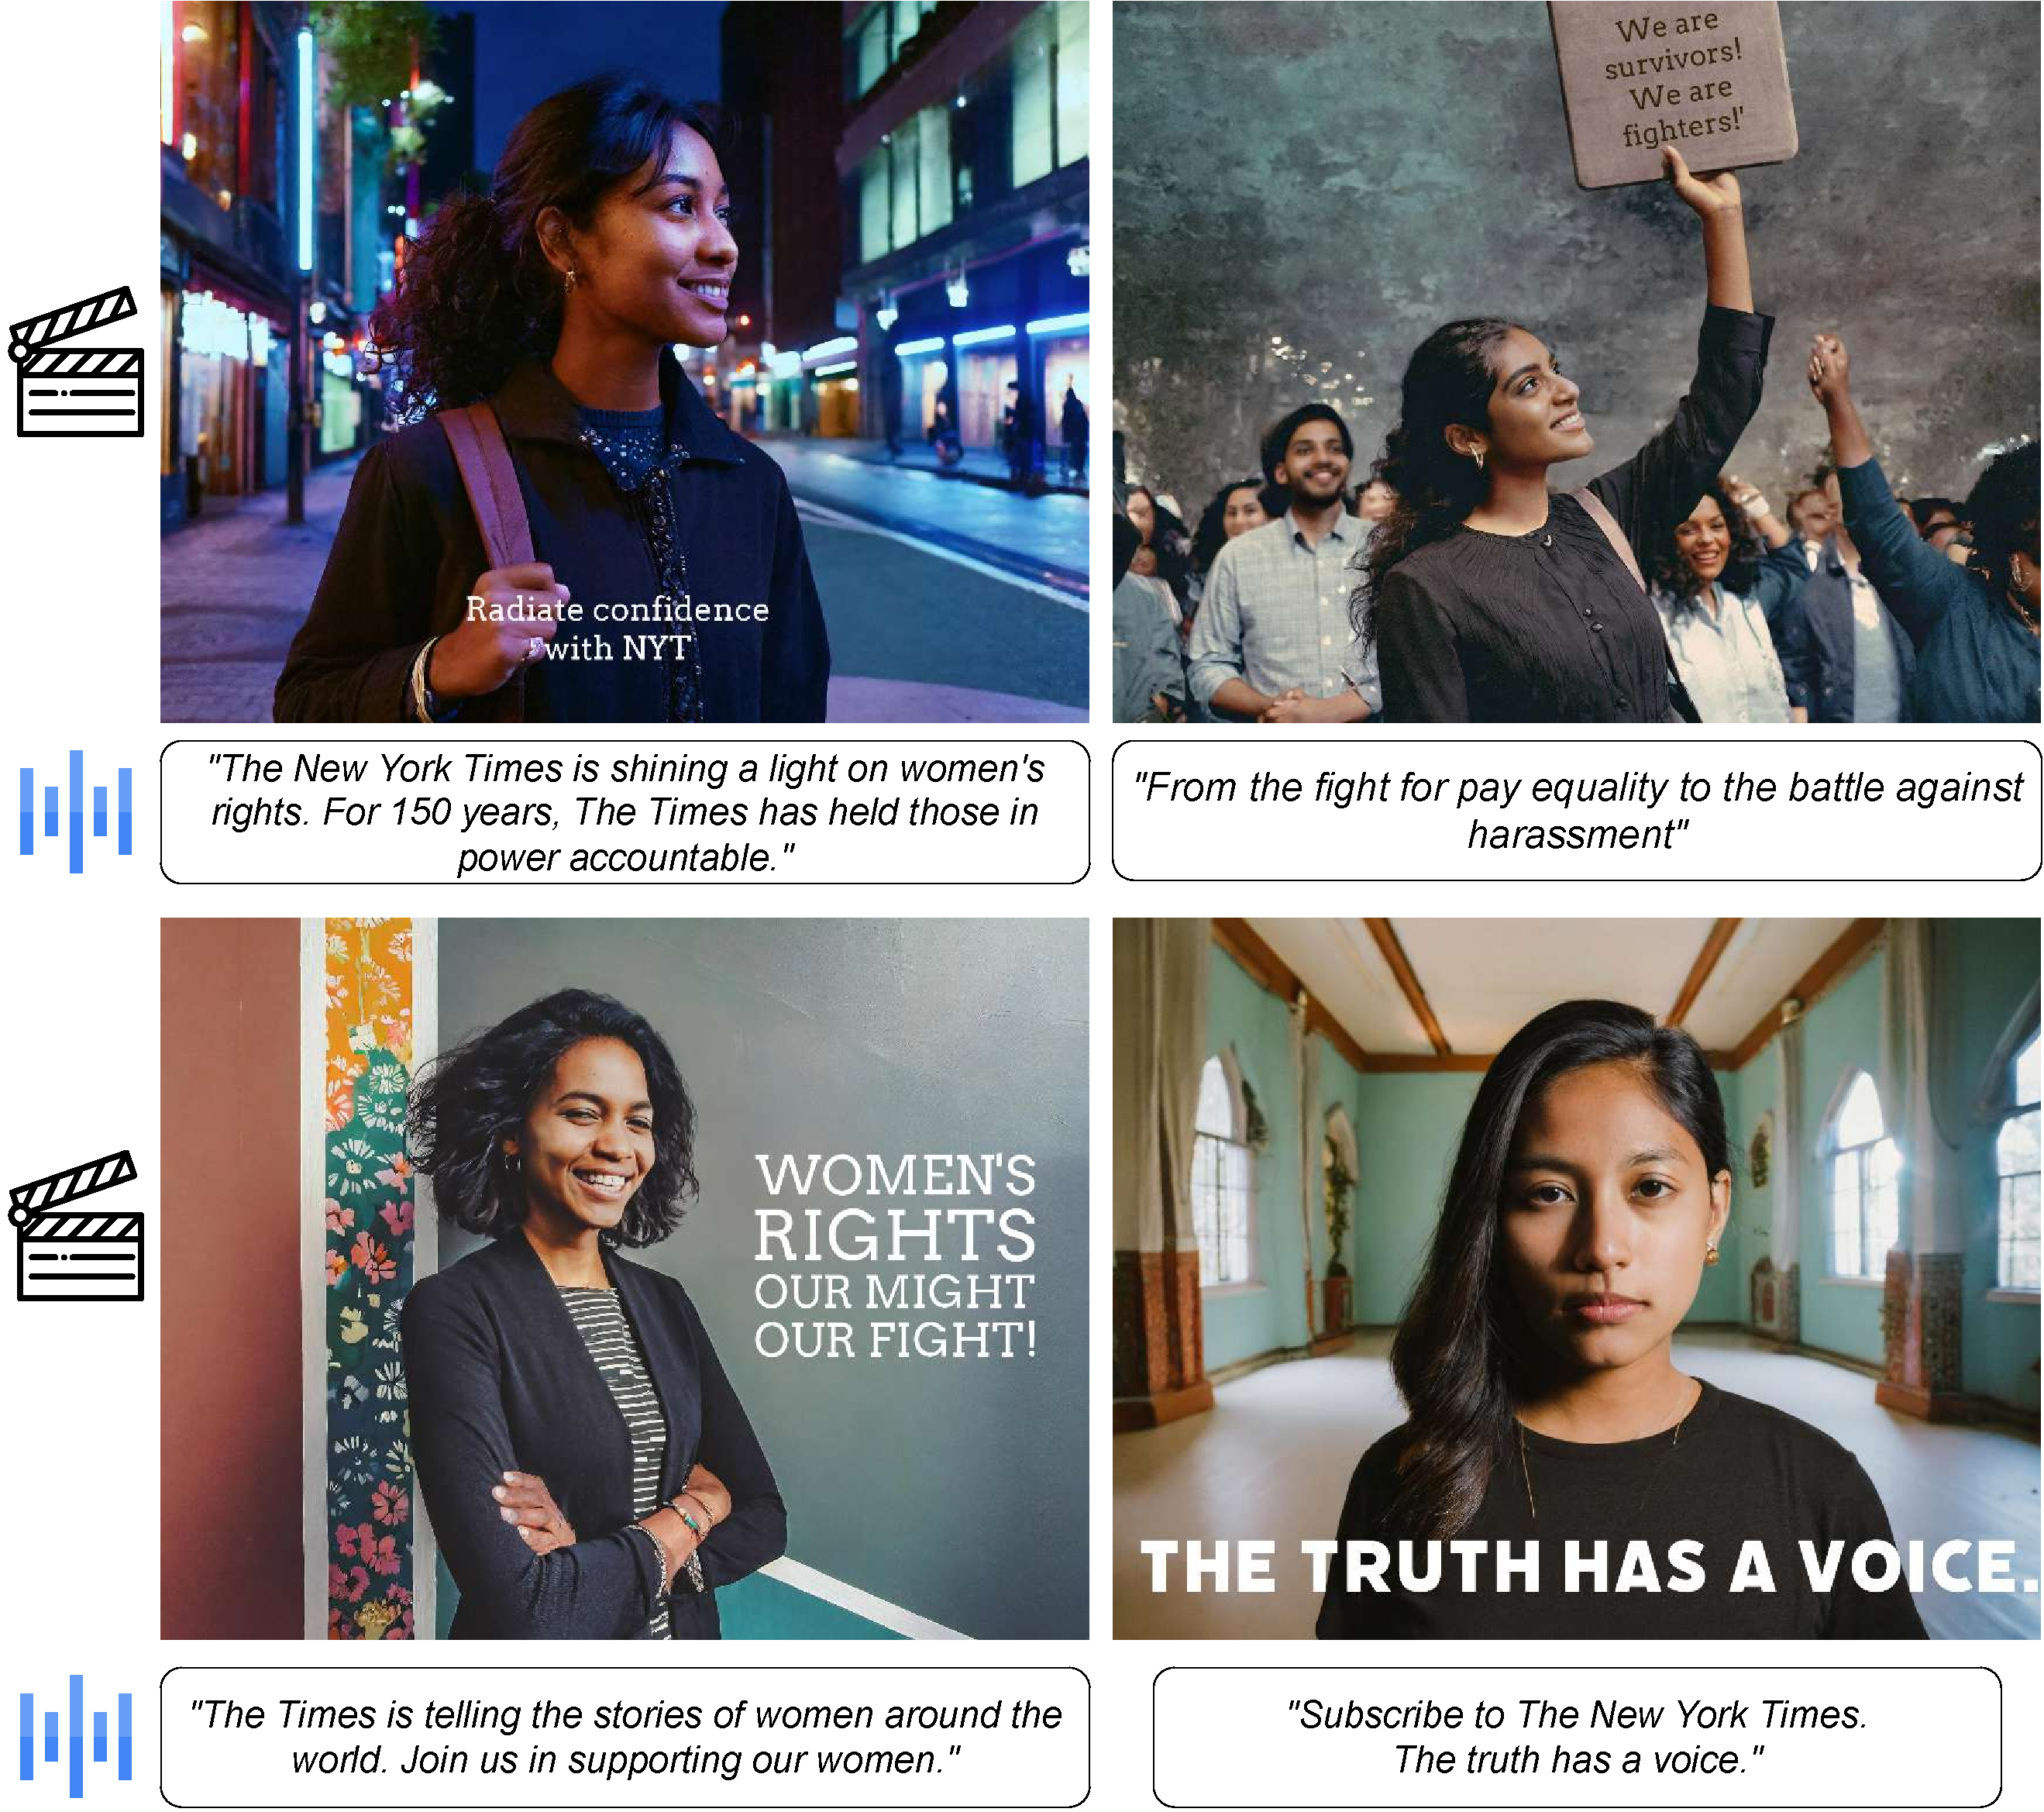
\includegraphics[width=0.95\textwidth]{images/henry/Henry-NYT.drawio_compressed.pdf}
    \caption{Henry-SEED Prompt: \textit{Generate the detailed description of a 50 second memorable advertisement titled "Shining a Light on Women’s Rights | The Truth Has a Voice | The New York Times" for the brand The New York Times} Link to the original ad: \url{https://www.youtube.com/watch?v=bPblzhUzTeg} Original memorability score: 65. Memorability score of Generated Ad: 91.}
    \label{fig:adgen-NYT}
\end{figure*}

%%%%%%%%%%%%%%%%%%%%%%%%%%%%%%%%%%%%%%%%%%


\subsection{Generation of Ads using Henry-SEED}
\label{sec:Generated Ad Samples}


Henry-SEED takes as input a prompt consisting of the title of the ad to be generated and the brand name and generates the scene-by-scene verbalization of cognitive and visual concepts and voiceover. Listings~\ref{lst:maytag}-\ref{lst:publix} gives the input and output of a few randomly chosen examples of advertisements generated by Henry-SEED are shown below. Using the output script generated by Henry-SEED, we next prompt Adobe Firefly \cite{adobefirefly} with Henry-SEED's output to generate the visualization. Next, OCR from the Henry-SEED generated verbalization is put on top of the generated images manually. We provide visualizations for easier understanding (Figs.~\ref{fig:brainly-generated-ad}-\ref{fig:maytag-generated-ad}), along with the raw generations (Listings~\ref{lst:maytag}-\ref{lst:publix}). 



\begin{figure*}[]
    \centering
    \includegraphics[width=0.95\textwidth]{images/henry/Henry-Maytag.drawio.pdf}
    \caption{Henry-SEED Prompt: \textit{Generate the detailed description of a 18 second memorable advertisement titled "Maytag Overnight Wash and Dry" for the brand Costco}. Link to the original ad: \url{https://www.youtube.com/watch?v=uT72lJhUUS0} Original memorability score: 76. Memorability score of the generated Ad: 83}
    \label{fig:maytag-generated-ad}
\end{figure*}



\begin{lstlisting}[caption={Advertisement generated by Henry-SEED for the Costco Ad. Original Ad: \url{https://www.youtube.com/watch?v=uT72lJhUUS0}},frame=single,breaklines=true,basicstyle=\tiny, label={lst:maytag}]
Input Title: "Maytag Overnight Wash and Dry" for the brand Costco


Generated Ad: "The ad is shot in landscape orientation, at a medium pace. 

Scene 1: The scene shows a person standing in front of a washer and dryer
Emotions: comforting, comfortable
Tags: appliance, laundry, laundry room, man
Voiceover: "Maytag has taken the laundry room by storm with their overnight wash and dry."
Colors: Gray, Off_White, Silver, White, Black, Dark_Gray

Scene 2: The scene shows a person lying on a bed pressing a button on a cell phone
Emotions: gift, birthday, holiday
Tags: button, catch, smartphone, hand
Voiceover: "Imagine going to bed with dirty clothes and waking up to a fresh, clean load. All without leaving the house. It's like having your own personal laundry assistant." 
Colors: Gray, Silver, Black, Dark_Gray, Dark_Brown

Scene 3: The scene shows a man and woman embracing while a washer and dryer are in the background
Emotions: love, happiness, togetherness
Tags: couple, hug, laundry, laundry room
Voiceover: "Never fight over the laundry room again."
Colors: Gray, Off_White, Silver, White,Black, Dark_Gray

Scene 4: The scene shows a logo of Maytag
Emotions: trust, confidence
Tags: logo, Maytag
Voiceover: "Get a Maytag and enjoy the luxury of time."
Colors: Off_White, Silver, White, Black, Dark_Gray, Gray
"
\end{lstlisting}



\begin{lstlisting}[caption={Advertisement generated by Henry-SEED for the Pruduential Financial Ad. Original Ad: \url{https://www.youtube.com/watch?v=JPfi0P-0nwU}},frame=single,breaklines=true,basicstyle=\tiny, label={lst:Prudential-financial-ad}]
Input Title:   "Financial Professional Tips: Planning for Your Own Care" for the brand Prudential Financial

Generated Ad: "The ad is shot in landscape orientation, at a low pace. 

Scene 1: The scene shows a woman looking thoughtfully at a laptop on her desk
Emotions: concern and contemplation
Tags: computer, laptop, office, woman
Colors: Gray, Dark_Blue

Scene 2: The scene shows the same woman now with a slight frown as she examines papers that appear to be medical bills
Emotions: worry and realization
Tags: bills, healthcare, paperwork, desk
Voiceover: "Long-Term Care is one of the most important issues in financial planning, but it's not always easy to talk about."
Colors: Gray, Dark_Blue

Scene 3: The scene shows the woman engaging in a conversation with a financial professional
Emotions: engagement and interest
Tags: consultation, financial advisor, discussion, office
Voiceover: "As a Financial Professional, I can help you evaluate your options and determine how much you may need to set aside each month."
Colors: Olive, Gray

Scene 4: The scene shows the woman in deep thought, looking out of a window while holding a pen and notepad, suggesting planning and reflection
Emotions: contemplation and seriousness
Tags: planning, reflection, window, notepad
Colors: Sky_Blue, Light_Gray

Scene 5: The scene transitions back to show the woman nodding in understanding as she listens to the financial professional, visibly gaining confidence
Emotions: comprehension and confidence
Tags: financial professional, office, learning, agreement
Voiceover: "Most people believe that they can rely on Medicare to pay for their long-term care expenses. But the truth is, Medicare typically only covers about 65% of the cost of a nursing home stay and only about 32% of the cost of an assisted living stay."
Colors: Gray, Dark_Blue

Scene 6: The scene shows the woman now jotting down notes actively, with a look of determination on her face
Emotions: determination and proactivity
Tags: planning, notetaking, strategy, office
Voiceover: "So if you're a typical American, you'll need about $100,000 to cover the remaining costs of long-term care."
Colors: Gray, Dark_Blue

Scene 7: The scene shifts to the woman shaking hands with the financial professional, symbolizing a plan set in motion
Emotions: satisfaction and trust
Tags: handshake, agreement, financial planning, commitment
Colors: Gray, Dark_Blue

Scene 8: The scene cuts to the woman now at home, relaxed and smiling, speaking on the phone, perhaps sharing her relief and positive steps taken with a loved one
Emotions: relief and happiness
Tags: home, communication, personal life, reassurance
Voiceover: "Let's talk about a plan for your own care."
Colors: Cream, Soft_Green

Scene 9: The final scene zooms out to a serene image of the woman walking in a park, symbolizing peace of mind about her future
Emotions: contentment and peace
Tags: park, walking, future, peace of mind"
Colors: Sky_Blue, Green
\end{lstlisting}





\begin{lstlisting}[caption={Advertisement generated by Henry-SEED for an Adidas Ad. Original Ad: \url{https://www.youtube.com/watch?v=fujboh-W7Sk}},frame=single,breaklines=true,basicstyle=\tiny, label={lst:adidas}]
Input Title:  "I'M POSSIBLE | IMPOSSIBLE IS NOTHING | Adidas" for the brand Adidas


Generated Ad: "The ad is shot in landscape orientation, at a medium pace.

Scene 1: The scene shows a man facing a rock climbing wall, poised to start his ascent
Emotions: anticipation and focus
Tags: athletic, climb, climber, rock
Voiceover: "What is possible is up to you."
Colors: Gray, Dark_Brown

Scene 2: The scene shows a man as he begins to climb, gripping the rock tightly
Emotions: determination and strain
Tags: athletic, climb, climber, hand
Voiceover: "Don't let anyone tell you otherwise."
Colors: Dark_Gray, Dark_Brown

Scene 3: The scene shows the man midway up the rock wall, reaching for a distant handhold
Emotions: perseverance and challenge
Tags: athletic, climb, climber, hand
Colors: Black, Dark_Gray

Scene 4: The scene captures a moment where the man slips but regains his grip on the rock face, muscles tensing
Emotions: tension and danger
Tags: athletic, climb, climber, hand
Colors: Dark_Gray, Dark_Brown

Scene 5: The scene shows the man pausing to chalk his hands, his breath visible in the cool air
Emotions: calm and preparation
Tags: athletic, chalk, climb, climber
Colors: Gray, Dark_Brown

Scene 6: The scene shows the man navigating a particularly difficult part of the climb, his movements precise and deliberate
Emotions: concentration and determination
Tags: athletic, climb, climber, hand
Colors: Black, Dark_Gray

Scene 7: The scene shows the climber's face, sweat beading on his forehead, reflecting the intensity of his effort
Emotions: grit and resolve
Tags: athletic, climb, climber, determination
Colors: Dark_Gray, Dark_Brown

Scene 8: The scene shows the man reaching for the final ledge, the clear sky behind him signaling the nearing end of his ascent
Emotions: anticipation and effort
Tags: athletic, climb, climber, hand
Voiceover: "Impossible is not an obstacle."
Colors: Dark_Gray, Gray, Dark_Brown, Blue

Scene 9: The scene shows the man pulling himself onto the summit, his body silhouetted against the sky
Emotions: triumph and exhilaration
Tags: athletic, climb, climber, hand
Voiceover: "It's a chance to prove them wrong."
Colors: Dark_Gray, Dark_Brown, Blue

Scene 10: The scene shows the man standing on top of the rock with his arms raised in victory, overlooking the landscape below
Emotions: achievement and elation
Tags: athletic, arms up, climb, climber"
Colors: Dark_Gray, Dark_Brown
\end{lstlisting}






\begin{lstlisting}[caption={Advertisement generated by Henry-SEED for an Amazon ad. Original Ad: \url{https://www.youtube.com/watch?v=rcFTqs-zSH4}},frame=single,breaklines=true,basicstyle=\tiny,label={lst:amazon}]

Input Title:  "Alexa Auto, Listening to Audiobooks" for the brand Amazon

Generated Ad: "The ad is shot in landscape orientation, at a low pace.

Scene 1: The scene shows a car driving down a country road near a mountain house
Emotions: anticipation, freedom
Tags: blue, car, drive, house
Colors: White, Lavender, Dark_Blue,Turquoise, Black

Scene 2: The scene shows an image of a car approaching a large sign above the road, signaling the start of the highway
Emotions: curiosity, readiness
Tags: car, drive, road sign, highway
Voiceover: "You just pulled onto the highway"
Colors: White, Lavender,Turquoise, Gray

Scene 3: The scene shows an in-car view with a driver's hands on the steering wheel, a smartphone mounted on the dashboard displaying the Amazon Music app
Emotions: concentration, engagement
Tags: car interior, hands, smartphone, technology
Voiceover: " but you can't remember the name of that band that's been stuck in your head all morning."
Colors: White, Dark_Blue,Black, Gray

Scene 4: The scene shows the driver speaking to Alexa through the car's infotainment system, the display lighting up in response
Emotions: interaction, ease
Tags: car interior, voice command, infotainment system
Voiceover: "With Alexa and Amazon Music, you don't have to remember.Just ask, "Alexa, play the Beatles."
Colors: White, Lavender, Dark_Blue, Black

Scene 5: The scene shows the car passing through a landscape with rolling hills and the sun beginning to set in the background
Emotions: satisfaction, serenity
Tags: car, drive, hills, sunset
Colors: White, Lavender, Turquoise, Dark_Blue

Scene 6: The final scene shows the vehicle driving into the horizon, as the iconic music of the Beatles fills the car's interior
Emotions: fulfillment, joy
Tags: car, drive, horizon, music"
Colors: White, Lavender, Orange, Dark_Blue
\end{lstlisting}




\begin{lstlisting}[caption={Advertisement generated by Henry-SEED for an Gatorade ad. Original Ad: \url{https://www.youtube.com/watch?v=BKPQkjRF4yY}},frame=single,breaklines=true,basicstyle=\tiny, label={lst:gatorade}]
Input Title:  "Gatorade | Make Your Own Footsteps with Suni Lee" for the brand Gatorade

Generated Ad: "The ad is shot in landscape orientation, at a medium pace.

Scene 1: The scene shows Sunisa Manado standing in front of her house
Emotions: determination, brave, confident, persistence, courage
Tags: athletic, face, girl, muscle
Voiceover: "I'm Sunisa Manado, but you can call me Sunisa. And I'm going to show you how I stay motivated. Let's go! This is my neighborhood. I'm going to take you through my favorite spots. There's my house right there."
Colors: Dark_Brown, Black, Brown, Tan

Scene 2: The scene shows Sunisa Manado performing a handstand in the park
Emotions: achievement, determination, persistence, commitment, success
Tags: balance, gymnast, handstand, girl
Voiceover: "And this is the park where I get so much done. This is the park where I train."
Colors: Dark_Brown, Dark_Blue, Purple, Gray

Scene 3: The scene shows Sunisa Manado doing a flip on the balance beam
Emotions: brave, courage, determination, persistence, inspiration
Tags: gymnast, flip, beam, girl
Voiceover: "Being an athlete takes a lot of hard work and determination."
Colors: Dark_Brown, Dark_Blue, Purple, Gray

Scene 4: The scene shows Sunisa Manado in a powerful pose in her pink sports bra and leotard
Emotions: determination, brave, courage, persistence, inspiration
Tags: athletic, face, girl, gymnast
Colors: Dark_Brown, Dark_Blue, Purple, Gray

Scene 5: The scene shows Sunisa Manado lifting herself on the parallel bars
Emotions: achievement, persistence, determination, courage, commitment
Tags: gymnast, lift, bars, girl
Voiceover: "And being an athlete also means that you have to have good nutrition."
Colors: Dark_Brown, Dark_Blue, Purple, Gray

Scene 6: The scene shows Sunisa Manado practicing her routine on the floor of the park
Emotions: determination, persistence, inspiration, commitment, discipline
Tags: floor, gymnast, routine, girl
Colors: Dark_Brown, Dark_Blue, Purple, Gray

Scene 7: The scene shows Sunisa Manado spinning on the balance beam
Emotions: success, brave, determination, precision, focus
Tags: beam, spin, gymnast, girl
Colors: Dark_Brown, Dark_Blue, Purple, Gray

Scene 8: The scene shows Sunisa Manado holding a bottle of Gatorade, rehydrating after her practice
Emotions: refreshed, healthy, satisfaction, wellbeing, recovery
Tags: athlete, drink, Gatorade, health
Voiceover: "That's why I choose to fuel up with Gatorade. You need to have that energy, especially during my toughest training."
Colors: Black, Dark_Green, Dark_Gray, Gray

Scene 9: The scene shows Sunisa Manado smiling towards the camera with a sense of pride and accomplishment
Emotions: joy, confidence, pride, optimism, accomplishment
Tags: face, smile, girl, gymnast
Voiceover: "Gatorade helps replenish what I've lost and helps keep me going."
Colors: Black, Dark_Green, Dark_Gray, Gray

Scene 10: The scene shows Sunisa Manado walking away from the park, as the sun sets, symbolizing the end of a day's hard work
Emotions: contemplation, fulfillment, anticipation, resilience, hope
Tags: sunset, walk, reflection, girl
Voiceover: "I'm going to make my own footsteps. Follow your dreams, but don't forget to chase your greatness."
Colors: Black, Dark_Green, Dark_Gray, Gray"
\end{lstlisting}


\begin{lstlisting}[caption={Advertisement generated by Henry-SEED for a Rolex ad. Original Ad: \url{https://www.youtube.com/watch?v=vA-Lxmh1MdQ}},frame=single,breaklines=true,basicstyle=\tiny, label={lst:rolex}]
Input Title: "Rolesor A Meeting of Metals" for the brand Rolex

Generated Ad: "The ad is shot in landscape orientation, at a low pace."

Scene 1: The scene shows a close up of a watch that is on a wrist
Emotions: anticipation, luxury, elegance
Tags: dial, gold, watch
Colors: Dark_Brown, Brown, Black, Khaki

Scene 2: The scene shows a gold and silver watch sitting on a table, reflecting soft light
Emotions: sophistication, status, success
Tags: dial, gold, watch
Colors: Brown, Dark_Brown, Khaki, Black

Scene 3: The scene shows a person's hands elegantly wrapping the gold and silver watch in delicate gift paper
Emotions: care, generosity, surprise
Tags: wrapping, gift, luxury
Colors: Brown, Khaki, Gold, White

Scene 4: The scene shows a recipient's joyous reaction as they receive the watch as a gift at a celebratory gathering
Emotions: happiness, gratitude, celebration
Tags: emotion, celebration, gift
Colors: Gold, Silver, Cream, Warm hues, Soft lighting

Scene 5: The scene shows the watch being worn at an elegant event, the gold and silver glinting under ambient lighting
Emotions: pride, accomplishment, refinement
Tags: elegance, luxury, watch
Colors: Gold, Silver, Black, Soft lighting, Dark hues
\end{lstlisting}

\begin{lstlisting}[caption={Advertisement generated by Henry-SEED for an NVIDIA ad. Original Ad: \url{https://www.youtube.com/watch?v=HnaOhOJ6AcM}},frame=single,breaklines=true,basicstyle=\tiny,label={lst:nvidia}]
Input Title: "Pac Man 256 on NVIDIA SHIELD" for the brand Nvidia

Generated Ad: "The ad is shot in landscape orientation, at a medium pace. "

Scene 1: The scene shows a black and white logo.
Emotions: danger, tough
Tags: brand, logo
The text shown in the scene is 'SHIELD'
Colors: Black, White, Gray

Scene 2: The scene shows a black screen with a red light on it
Emotions: danger, tough
Tags: brand, logo, text
The text shown in the scene is 'SHIELD'
Colors: Black, White, Red

Scene 3: The scene shows a computer screen showing a game of Pac-Man
Emotions: nostalgia, fun
Tags: arcade, arcade machine, game, Pac-Man
The text shown in the scene is 'HIGH SCORE'
Colors: Cyan, Yellow, Gray, Dark Green, Red

Scene 4: The scene shows a video game character navigating a maze filled with obstacles
Emotions: excitement, challenge
Tags: arcade, character, game, maze
The text shown in the scene is 'LEVEL UP'
Colors: Cyan, Red, Pink, Orange, Gray

Scene 5: The scene shows a video game with a racing theme, cars zooming on the track
Emotions: thrill, speed
Tags: racing, cars, game, screenshot
The text shown in the scene is 'NEW RECORD'
Colors: Red, Yellow, Blue, Gray, Black

Scene 6: The scene shows a strategy video game with a detailed world map
Emotions: focus, strategy
Tags: strategy game, world map, empire, video game
The text shown in the scene is 'EXPAND YOUR EMPIRE'
Colors: Green, Brown, Blue, White, Tan

Scene 7: The scene shows a futuristic virtual reality game with immersive graphics
Emotions: amazement, innovation
Tags: VR, virtual reality, future, game
The text shown in the scene is 'ENTER NEW WORLDS'
Colors: Neon Blue, Neon Green, Black, Dark Blue

Scene 8: The scene shows a family gathered around playing a multiplayer video game, laughing and enjoying
Emotions: joy, togetherness
Tags: family, multiplayer, game, living room
The text shown in the scene is 'PLAY TOGETHER'
Colors: Multi-colored, Warm Hues

Scene 9: The scene transitions to a player wearing headphones, deeply concentrated in an esports competition
Emotions: determination, competition
Tags: esports, competition, gamer, video game
The text shown in the scene is 'RISE TO THE CHALLENGE'
Colors: Black, Neon, Dark, Spotlights

Scene 10: The scene closes with the NVIDIA SHIELD logo emerging brightly on the screen
Emotions: empowerment, assurance
Tags: brand, logo, closing
The text shown in the scene is 'NVIDIA. SHIELD - Game Your Way'
Colors: Red, White, Black
\end{lstlisting}

\begin{lstlisting}[caption={Advertisement generated by Henry-SEED for a Zillow ad. Original Ad: \url{https://www.youtube.com/watch?v=P6gydrvTkaA}},frame=single,breaklines=true,basicstyle=\tiny, label={lst:zillow}]
Input Title: "Find It, Tour It and Own It With Zillow (:06)" for the brand Zillow

Generated Ad: "The ad is shot in landscape orientation, at a medium pace.

Scene 1: The scene shows a person holding a cell phone with their hand.
Emotions: achievement, ambition
Tags: catch, smartphone, hand, person, phone, screen, text message, woman
Colors: Gray, Dark_Blue, Dark_Brown, Dark_Pink, Off_White

Scene 2: The scene shows a woman in a sweater looking at a cell phone.
Emotions: happy, smile
Tags: smartphone, earphone, girl, person, smile, woman
Colors: Gray, Dark_Brown, Dark_Pink, Dark_Blue

Scene 3: The scene shows a woman looking at a phone with a map on it.
Emotions: confident, smiling
Tags: catch, smartphone, earphone, girl, person, phone, stand, talk, woman
Colors: Gray, Dark_Brown, Dark_Pink, Dark_Blue

Scene 4: The scene shows a woman looking at a cell phone with a real estate app on it.
Emotions: togetherness, happiness
Tags: smartphone, earphone, girl, person, woman
Colors: Gray, Dark_Brown, Dark_Pink, Dark_Blue

Scene 5: The scene shows a woman looking at a cell phone with a real estate app displayed.
Emotions: happy, smiling
Tags: smartphone, earphone, girl, person, woman
Colors: Gray, Dark_Brown, Dark_Pink, Dark_Blue

Scene 6: The scene shows a woman using a cell phone to speak with an agent.
Emotions: confident, happy
Tags: smartphone, earphone, girl, person, talk, woman
Colors: Gray, Dark_Brown, Dark_Pink, Dark_Blue
Voiceover: "Getting the perfect home is a journey, so we help you find it, tour it, and own it."

Scene 7: The scene shows a woman completing a transaction on a cell phone.
Emotions: achievement, satisfied
Tags: smartphone, earphone, girl, person, woman
Colors: Gray, Dark_Brown, Dark_Pink, Dark_Blue"
Voiceover:  "For moving made simple, there's no place like Zillow"
\end{lstlisting}

\begin{lstlisting}[caption={Advertisement generated by Henry-SEED for a Kroger ad. Original Ad: \url{https://www.youtube.com/watch?v=SqwqI01q3fA}},frame=single,breaklines=true,basicstyle=\tiny, label={lst:kroger}]
Input Title: "How to Make Taco Seasoning | Kroger Recipes | Kroger" for the brand Kroger

Generated Ad: "The ad is shot in landscape orientation, at a low pace.  

Scene 1: The scene shows a person pouring chipotle adobo sauce into a glass jar.
Emotions: care, comfort
Tags: bottle, can, container, hand, food, person, jar, liquid, pepper, pour, red, sauce, tomato sauce, tin, tray, woman
Colors: Black, Gray, Dark_Brown, Maroon, Dark_Red
Voiceover: "The audio in the ad says Taco seasoning is one of those spices that everyone loves on their food. It's so delicious and it's so easy to make."

Scene 2: The scene shows a woman in a red sweater adding ground cumin to the mix.
Emotions: anticipation, focus
Tags: blender, container, food, hand, person, ingredient, measuring cup, spice, woman
Voiceover: "All you have to do is get your chopstick and add some of the garlic and some of the onion and some of the cumin"
Colors: Black, Gray, Dark_Brown, Maroon, Dark_Red

Scene 3: The scene shows the addition of chili powder to the seasoning mix.
Emotions: precision, satisfaction
Tags: blender, container, food, food processor, hand, person, ingredient, mixture, spice, woman
Voiceover: " and some of the dried chilies and some of the oregano and some of the salt"
Colors: Black, Gray, Dark_Brown, Dark_Pink, Maroon

Scene 4: The scene shows the woman sprinkling crushed red pepper into the mix.
Emotions: excitement, zeal
Tags: blender, container, food, food processor, hand, person, ingredient, measuring cup, mixture, spice, woman
Voiceover: "and some of the paprika and some of the pepper and just give it a little bit of a squeeze"
Colors: Black, Gray, Dark_Brown, Maroon, Dark_Red

Scene 5: The scene shows the woman measuring and adding ground oregano to the seasoning mix.
Emotions: happiness, creativity
Tags: blender, container, food, food processor, hand, person, ingredient, measuring cup, mixture, spice, woman
Colors: Black, Gray, Dark_Brown, Maroon, Dark_Red

Scene 6: The scene shows the final steps of making the taco seasoning mix, with the woman adding garlic powder and onion powder.
Emotions: accomplishment, pride
Tags: blender, container, food, food processor, hand, person, ingredient, mixture, spice, woman
Voiceover: "You're going to taste it, so don't be afraid to add more or less of any of these ingredients, depending on how spicy or how flavorful you want your taco seasoning to be."
Colors: Black, Gray, Dark_Brown, Maroon, Dark_Red"

\end{lstlisting}


\begin{lstlisting}[caption={Advertisement generated by Henry-SEED for a Publix ad. Original Ad: \url{https://www.youtube.com/watch?v=HH0VWvs-cFg}},frame=single,breaklines=true,basicstyle=\tiny, label={lst:publix}]
Input Title: "GreenWise Ice Cream Scoop from Publix" for the brand Publix Supermarkets

Generated Ad: "The ad is shot in landscape orientation, at a low pace. 

Scene 1: The scene shows a woman standing in front of a refrigerator.
Emotions: anticipation, satisfaction
Tags: beverage, bottle, catch, doorway, drink, fill, girl, home appliance, juice, laugh, pour, refrigerator, shirt, stand, woman
Voiceover: "Greenwise, the better energy choice from Publix."
Colors: Black, Gray, Dark_Gray, Dark_Brown, Silver

Scene 2: The scene shows a woman holding a roll of Greenwise ice cream in her hand.
Emotions: curiosity, interest
Tags: bottle, catch, hand, woman
Voiceover: " All the deliciousness of ice cream, a fraction of the calories. And now it comes in a roll."
Colors: Black, Gray, Dark_Gray, Dark_Brown

Scene 3: The scene shows the woman as she easily scoops the ice cream onto a plate, displaying the convenience of the new roll format.
Emotions: ease, delight
Tags: plate, roll, scoop, serve, woman
Voiceover: " So you can easily scoop and serve exactly what you need."
Colors: Black, Gray, Dark_Gray, Dark_Brown

Scene 4: The scene shows the woman enjoying a bite of the Greenwise ice cream, her expression reflecting the product's deliciousness.
Emotions: enjoyment, satisfaction
Tags: bite, enjoyment, ice cream, satisfaction, taste, woman
Voiceover: "It's a win-win. Learn more at publix.com."
Colors: Black, Gray, Dark_Gray, Dark_Brown"

\end{lstlisting}

\begin{comment}
        
    \begin{adjustbox}{width=\textwidth, frame}
    \begin{lstlisting}[caption={Voiceover generated by Henry for an Ulta Beauty Ad}, label={lst:ulta}]
    Original Link to the video ad: https://memorability.blob.core.windows.net/videos/2506_lgJRPZy4ytY.mp4
    Input Title: How to Avoid Lice with Rosemary Repel by Fairy Tales | Ulta Beauty
    
    Generated Ad: "Unveil the secret to lice-free bliss with Rosemary Repel by Fairy Tales. 
    Immerse yourself in a tub of serenity, surrounded by products that promise a worry-free 
    experience. Feel the joy as smiles are exchanged, sharing the magic of Fairy Tales in 
    your home. Witness happiness in every jar, as the woman smiles, holding the key to a 
    carefree life. Embrace the enchantment of Ulta Beauty, where beauty meets wellness, 
    and worry fades away."
    \end{lstlisting}
    \end{adjustbox}
    
    
    
    \begin{adjustbox}{width=\textwidth, frame}
    \begin{lstlisting}[caption={Voiceover generated by Henry for a Home Depot Ad}, label={lst:homedepot}]
    Original link to the video ad: https://memorability.blob.core.windows.net/videos/1926_6V7nBPul4wE.mp4
    Input Title: Husky Folding Workbench | Garage Storage Ideas
    
    
    Generated Ad: "Transform your garage into more than just a parking space with the Husky 
    Folding Workbench. Crafted with durable steel and a sleek wood top, this workbench is 
    not only sturdy but stylish too. Whether you prefer working sitting or standing, its 
    adjustable height caters to your needs. And when the job is done, it folds flat, 
    saving precious floor space. With a lifetime warranty, it's time to take charge of 
    your workspace. Get smart and tough storage solutions from Home Depot, quality that lasts 
    since 1924."
    \end{lstlisting}
    \end{adjustbox}
\end{comment}

\begin{comment}    
    \begin{figure}[h]
    %\vspace{-0.8in}
        \centering
        \includegraphics[width=0.99\textwidth]{images/RLHF_1.pdf}
        \label{fig:Generation Architecture}
        \caption{Architecture of Henry for Memorable Ads Generation, this diagram shows three parts 1.UltraLAMBDA Reward Dataset Curation, We use Henry for Memorability simulation to curate a large scale reward dataset. 2. Preference Finetuning, These samples are combined with Filtered high memorability samples for Preference Fine Tuning 3. ILQL for Memorable ad generation using UltraLAMBDA \vspace{-2mm}\label{fig:Henry for memorable ad generation}}
        
    \end{figure}
\end{comment}



\begin{figure}
    \centering
    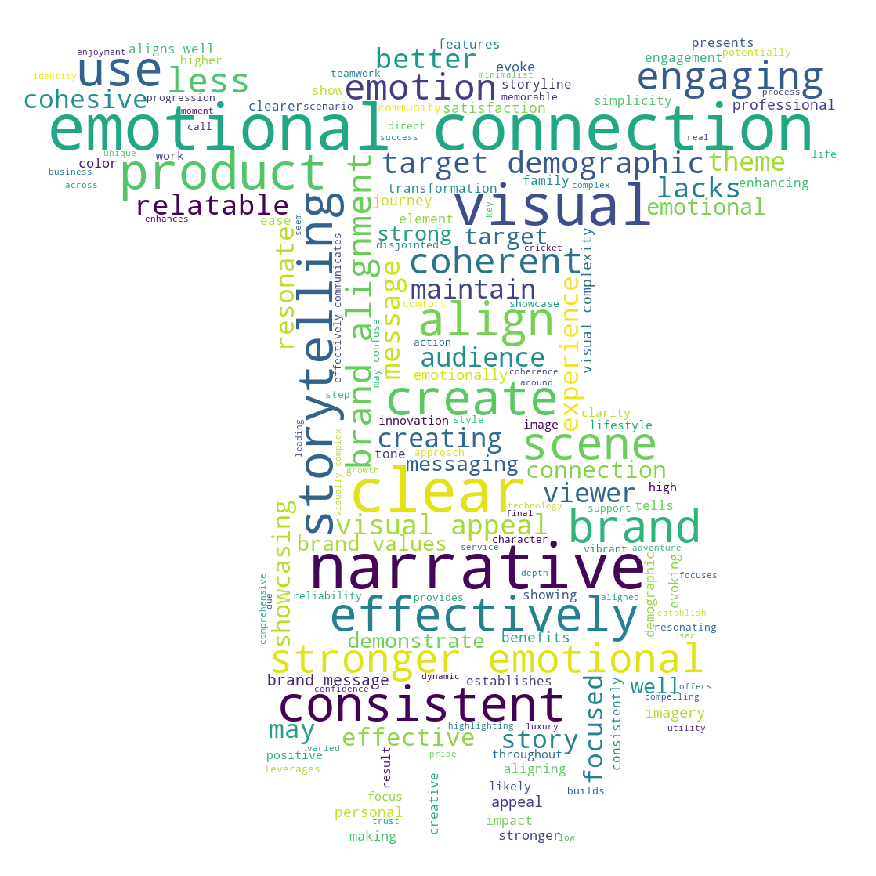
\includegraphics[width=0.5\textwidth]{images/henry/wordcloud_henry_win.pdf}
    \caption{Word Cloud (resembling Henry) for the GPT-4 reasoning on the 75/88 generations where it rates Henry-SEED Generated Ads to be better than the Original.}
    \label{fig:gpt4-henry-win-wordcloud}
\end{figure}

%%%%%%%%%%%%%%%%%%%%%%%%%%%%%%%%%%%%%%%%%%
%%%%%%%%%%%%%%%%%%%%%%%%%%%%%%%%%%%%%%%%%%

\FloatBarrier
\subsection{Extraction And Use Of Cognitive And Perceptual Signals In Advertisements}


\begin{landscape}
    
\begin{table*}[h]
%\vspace*{-1cm}
\begin{center}\small
\resizebox{1.5\textwidth}{!}{%
 \begin{tabular}{cp{1.8cm}p{5.5cm}p{1.5cm}p{5.5cm}}
     \toprule
     \small
      Image & Semantic Category & Verbalization & Semantic Category & Verbalization\\ 
    \cmidrule(r){1-1}\cmidrule(lr){2-2}\cmidrule(l){3-3}\cmidrule(l){4-4}\cmidrule(l){5-5}
     \multirow{10}{*}{\raisebox{-\totalheight}{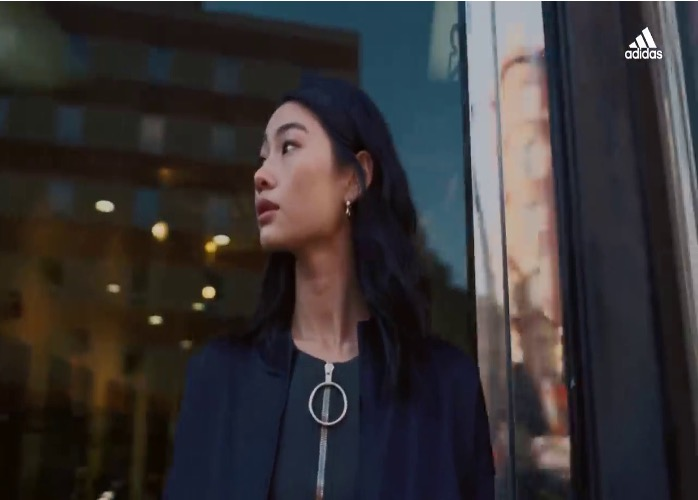
\includegraphics[width=0.25\columnwidth]{images/adidas-picture.jpg}}} & \textbf{OCR} & The text shown in the scene is ``\textcolor{red}{Adidas}''. & \textbf{Clutter} & The clutter in the scene is \textcolor{red}{low}.\\
    & \textbf{ASR} & The audio in the scene is ``\textcolor{red}{To take hold of the world’s spotlight overnight}''.& \textbf{Photo Style} & The photography style of the scene is \textcolor{red}{commercial photography}.\\
    & \textbf{Human Presence} & The scene has \textcolor{red}{1 person with prominent face}.& \textbf{Emotion} & The emotion of the scene is \textcolor{red}{ambitious, determined}.\\

    & \textbf{Caption} & The scene shows \textcolor{red}{a young woman sitting in a glass door looking out}.    & \textbf{Aesthetics} & The image has \textcolor{red}{medium} aesthetic value.\\
    & \textbf{Colors} & The foreground colors of the scene are \textcolor{red}{Black, Dark Brown, Dark Blue, Dark Gray, Mud Green} and the background colors are \textcolor{red}{Dark Blue, Black, Dark Brown}. The dominant tone of the scene is \textcolor{red}{neutral}.
    & \textbf{Object Tags} & This scene is categorized by the tags: \textcolor{red}{person, woman,  blazer, facing, template, fashion, street fashion, cold, client, cardigan, sweat}.\\
    & \textbf{Audio Type} & The scene has \textcolor{red}{music and speech}. & \textbf{Logo Presence} & There is \textcolor{red}{a logo} in the scene.\\\hline
  \end{tabular}}
  \caption{To augment the scene understanding of LLM, we verbalize video scenes and images using a diverse set of cognitive and perception tools and pass it to the LLM in the format shown in the table. For image memorability datasets, we use the following semantic categories: caption, color, photo style, emotion, clutter, human presence, object tags, OCR, and aesthetics. For video scene memorability datasets, we use the following semantic categories: caption, color, emotion, human presence, object tags, ASR, OCR, Audio-type, Logo-presence. We use the following models to extract the features: OCR \protect\cite{du2020pp}, clutter \protect\cite{khurana-etal-2023-synthesizing}, ASR \protect\cite{radford2022robust}, Photo style \protect\cite{li2023blip}, human presence \protect\cite{liu2023grounding}, emotion \protect\cite{singh2024llava}, caption \protect\cite{li2023blip}, aesthetics \protect\cite{ke2023vila}, colors \protect\cite{Qin_2020_PR}, object tags \protect\cite{zhang2023recognize}, audio-type \protect\cite{giannakopoulos2015pyaudioanalysis}, and logo presence \protect\cite{zhang2023recognize}. Black colored text is the verbalization template, and \textcolor{red}{red} text indicates the model outputs.
  \label{table:scene-verbalization-format}}
\end{center}
\end{table*}


\end{landscape}



\begin{figure}[]
    \centering
    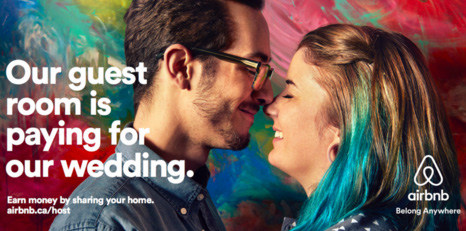
\includegraphics[width=0.48\textwidth]{images/airbnb.png}
    \caption{Airbnb advertisement showing the visual concepts of two adults, and the text ``Our guest room is paying for our wedding''. ``World knowledge'' captured by LLMs helps identify the two adults as partners, and helps relate the text with the two adults and the Airbnb logo to infer what the ad is talking about.}
    \label{fig:airbnb-ad}
\end{figure}

% : add analysis about embeddings of LM, HM, MM from Henry-SEED

\begin{figure*}[]
%\vspace{-0.8in}
    \centering
    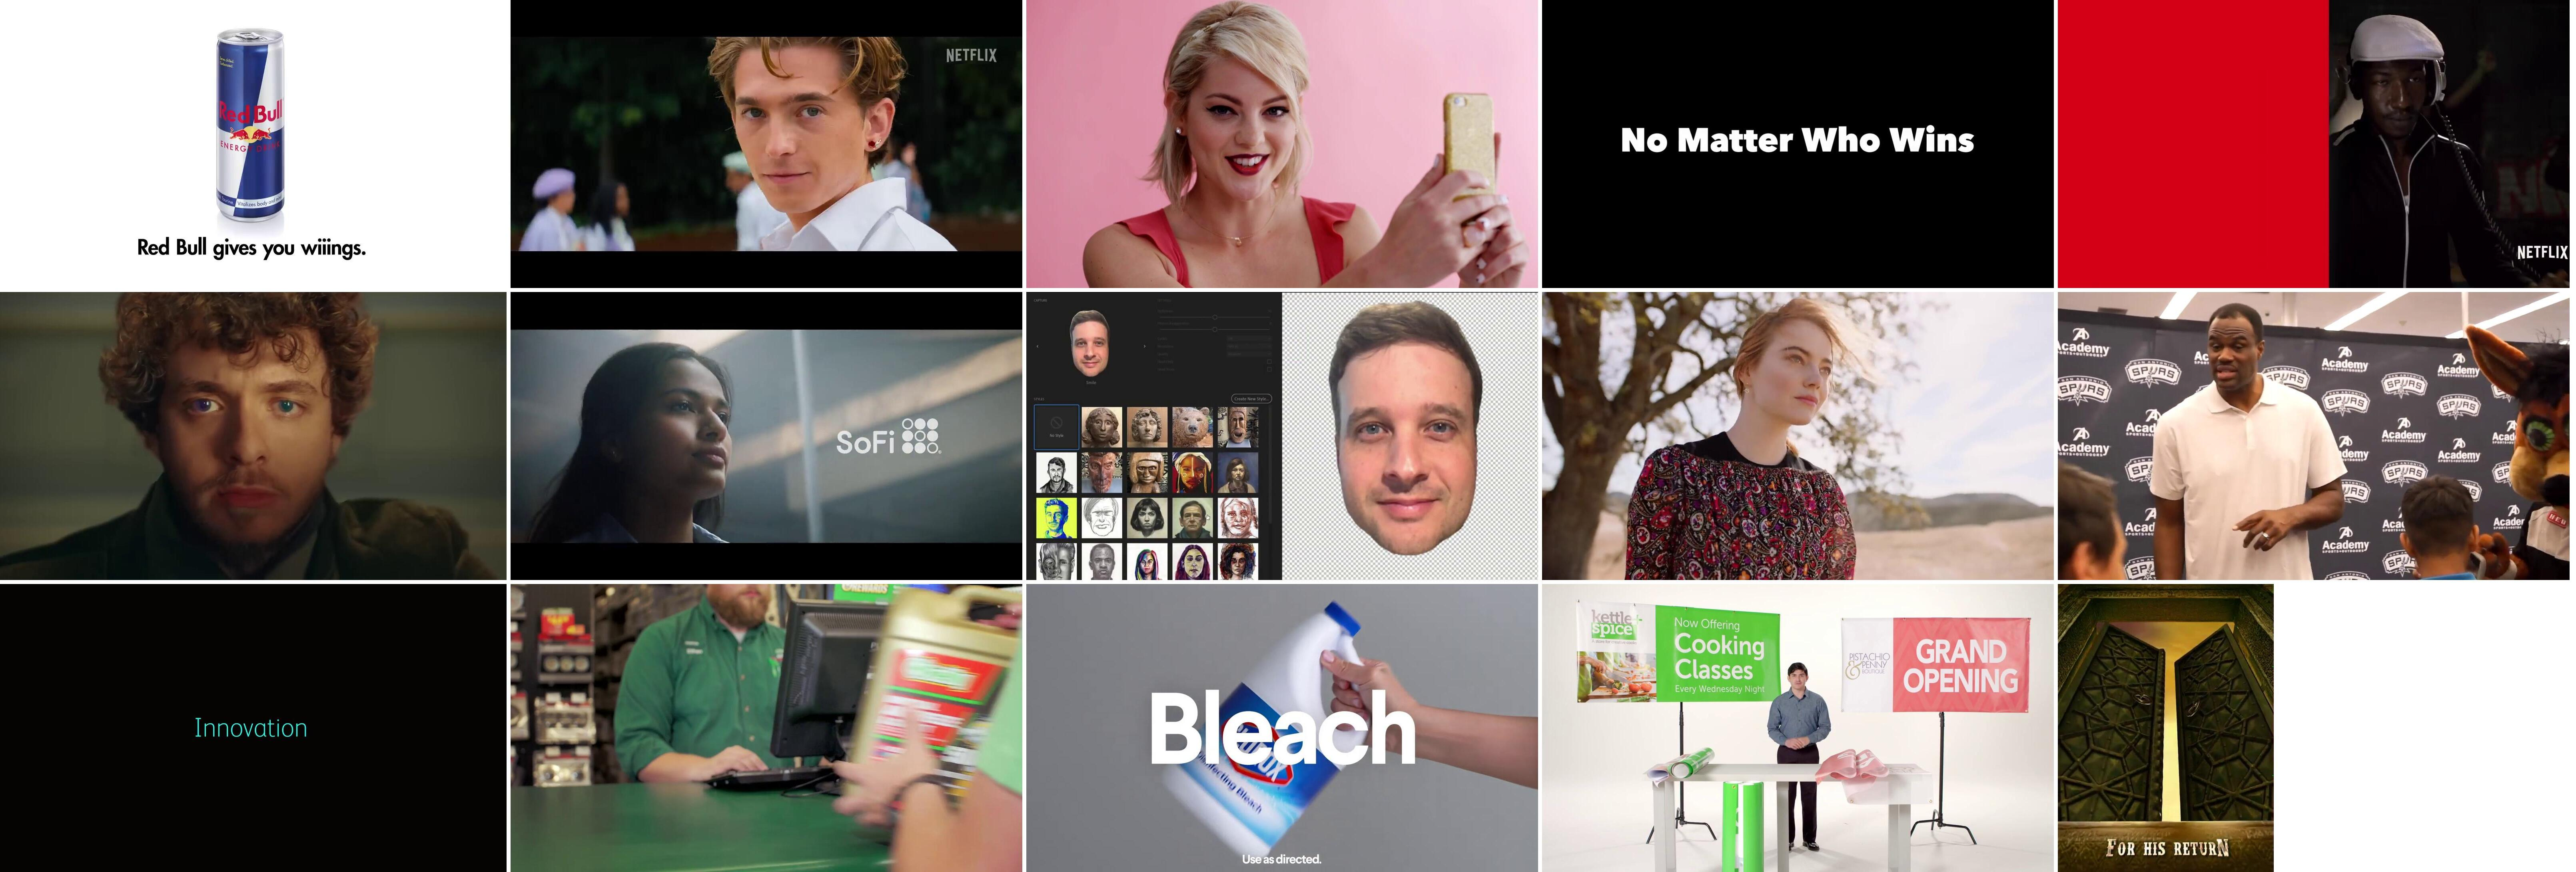
\includegraphics[width=0.99\textwidth]{images/collage.jpg}
%\end{figure}
%\begin{figure}[!t]
    \centering
    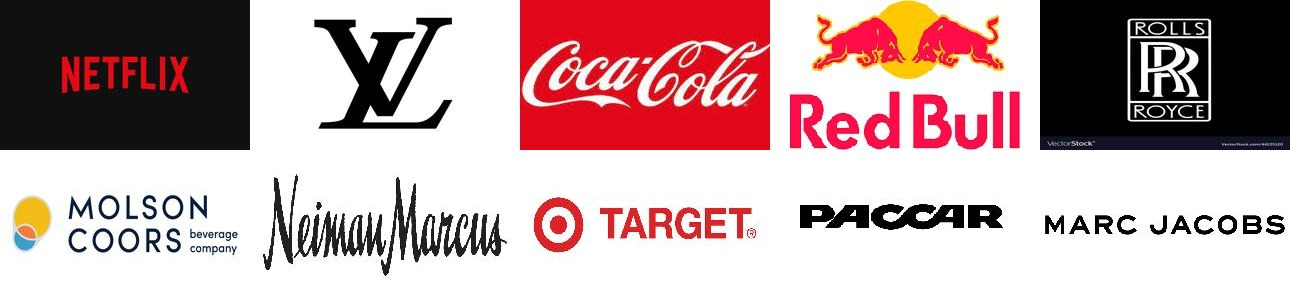
\includegraphics[width=0.99\textwidth]{images/brands.jpg}
    \caption{The top three rows show the keyframes from videos in our dataset, LAMBDA, arranged from most to least memorable. The bottom two rows show brands arranged from the most memorable brands to the least. 
    %\vspace{-2mm}
    }
    \label{fig:Memorable brands}
\end{figure*}


\FloatBarrier
\subsection{Ablation Experiments}
\begin{figure*}[]
%\vspace{-0.8in}
    \centering
    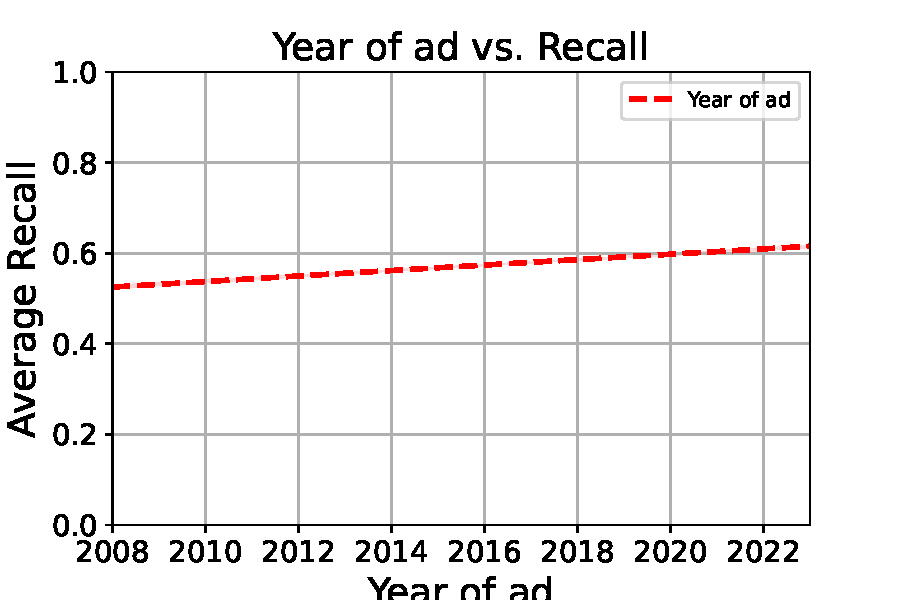
\includegraphics[width=0.8\textwidth]{images/year.pdf}
    \label{fig:memorabilityvides}

    \caption{The graph shows the relationship of the year the ad is uploaded on youtube vs the recall. 
    }
    \label{fig:Year}
\end{figure*}


\begin{table*}[!h]
%\vspace*{-1cm}
\centering
\resizebox{1.0\textwidth}{!}{%
\begin{tabular}{l|ll|llllllll}
\hline
\textbf{\makecell[l]{Generalization\\Type}} &  \textbf{Train on} & \textbf{\makecell[l]{Zero-shot\\Testing}} & \textbf{Lamem} & \textbf{Memcat} & \textbf{SUN} & \textbf{VideoMem} & \textbf{Memento10k} & \textbf{LAMBDA} \\ \hline
Memory-type & Short-term & Long-term & - &-        &-     & 0.31         & - & 0.18          \\
Memory-type & Long-term & Short-term &0.06       &0.08        &0.07     &0.15          &0.1         &-           \\
Modality & Videos  & Images &0.55     &0.65        &0.55     &-          &-         &-           \\
Modality & Images & Videos              &-       &-        &-     &0.44          &0.54         &0.09           \\
Brands & \makecell[l]{All except\\20 brands} & \makecell[l]{Left-out\\20 brands} &-       &-        &-     &-          &-           &0.42           \\
Dataset & \makecell[l]{All except\\Memento} & Memento &-      &-        &-     &-         & 0.59           &-           \\
Dataset & \makecell[l]{All except\\Memcat} & Memcat   &-       &0.68        &-     & -         &-         & -          \\\hline
\end{tabular}%
}
\caption{Ablation across data to understand how memorability prediction generalizes across the type of memory, datasets, modality (image/video), and brands. The reported values are correlations between model and human memorability scores. A few trends can be observed from the table: (i)~STM generalizes better on LTM in zero-shot than vice versa (rows 1 and 2), (ii)~Henry trained on either videos or images generalizes to both (rows 3 and 4), (iii)~There is a significant performance loss in modeling memorability for brands not seen during training (row 5), (iv)~Zero-shot generalization to Memento (video) and Memcat (image) is near to the current trained state of the art literature models on Memento \cite{Dumont_2023_CVPR} and Memcat \cite{hagen2023image} (rows 6 and 7).}
\label{table:data-ablation}
\end{table*}





\begin{table*}[!h]
\centering
\resizebox{0.99\textwidth}{!}{%
\begin{tabular}{lllllll}
\hline

& \textbf{Lamem} & \textbf{Memcat} & \textbf{VideoMem(ST)} & \textbf{Memento10k}  & \textbf{VideoMem(LT)}  & \textbf{LAMBDA} 
\\ \hline
\makecell[l]{Henry on\\individual datasets} & 0.74 & 0.82   &0.64 & 0.75  & 0.48   & 0.55  \\
Henry vision only &0.20       & 0.17       &0.17       &0.21        &0.15         &0.11  \\
Henry language only &0.51       & 0.53       &0.42       &0.54        &0.37         &0.44  \\
Henry -object tags &0.67       &0.71        &0.57       &0.69       &0.46         &0.52         \\
Henry -colors &0.65       &0.74        &0.55      &0.67       &0.45         &0.51         \\
Henry -emotion &0.71       &0.78        &0.61      & 0.73       &0.42         & 0.46         \\
Henry -aesthetics &0.72       &0.79        &0.61       &0.71       &0.46         &0.53         \\
Henry -clutter &0.73       &0.81        &0.60       &0.74       &0.45         &0.53     \\
Henry -asr &-       &-        &-       & -       &-         & 0.46         \\
Henry -asr-emotion &-       &-        &-       & -       &-         &0.42         \\
Henry on Silent Ads&-       &-        &-       & -       &-         &0.56        \\
\makecell[l]{Henry on Ads\\with audio}&-       &-        &-       & -       &-         &0.52        \\

\hline%\vspace{-3mm}
\end{tabular}%
}
\caption{Ablation across architectural choices. ``-'' denotes non-speech dataset. A few trends are visible from the table: (i)~Despite having a vision branch, object tags and colors have a net positive impact on the overall performance (rows 2,3,4), (ii)~For LTM (LAMBDA, VideoMem (LT)), dropping cognitive features such as emotion, aesthetics, and clutter cause a larger performance drop than dropping visual features such as objects and colors. The trend is the opposite for STM (Lamem, Memcat, VideoMem (ST), Memento10k).}
\label{table:architecture-ablation}
\end{table*}





\begin{figure*}[t]
    \centering
    \begin{subfigure}{0.75\textwidth}
        \centering
        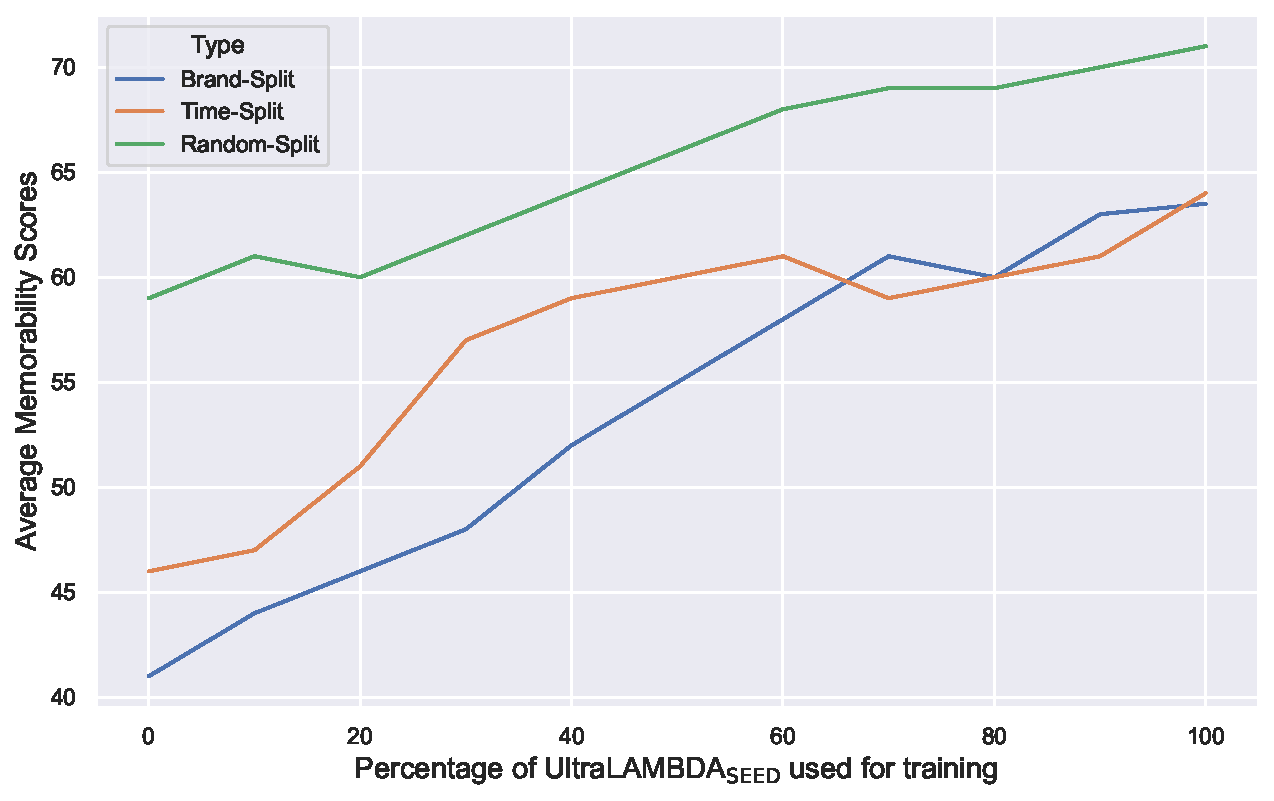
\includegraphics[width=\textwidth]{images/henry/memorability.pdf}
        \label{subfig:mem vs synthetic data}
        \caption{}
    \end{subfigure}
    \\
    \begin{subfigure}{0.75\textwidth}
        \centering
        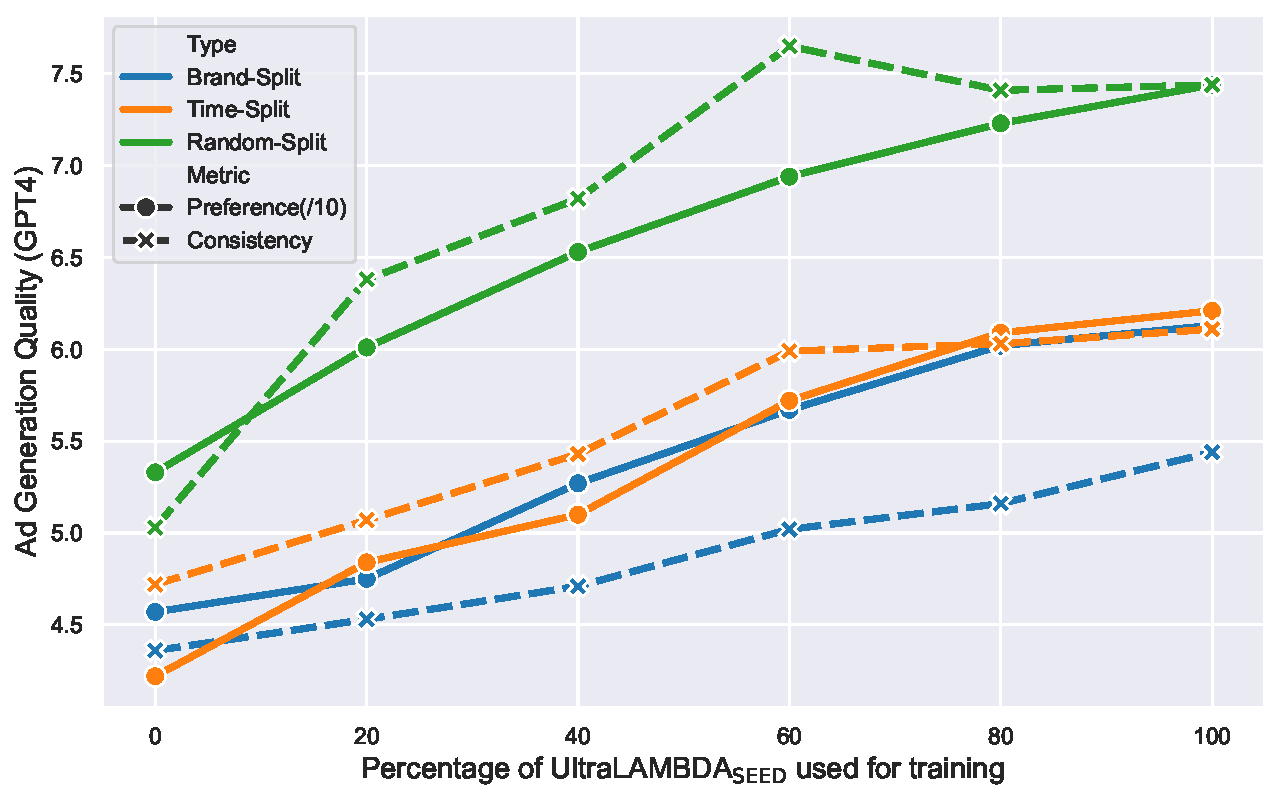
\includegraphics[width=\textwidth]{images/henry/adquality.pdf}
        \label{subfig:ad-quality vs synthetic data}
        \caption{}
    \end{subfigure}
    \caption{Graphs showing the importance of the amount of synthetic data on (a)~Ad memorability score and (b)~Ad quality for the generated ads. As we can see from the graphs, both the ad memorability and quality increase with the increase in the amount of synthetic data. \label{fig:synthetic-data-vs-generation-performance-1}}
\end{figure*}



\begin{table}
\centering
\begin{tabular}{l|l|l}
\hline
Task    & LAMBDA ($\rho$) & $\Delta$ Memorability \\\hline
BS-only & 0.541 & - \\
CS-only & - & +28.41 \\
BS+CS   & 0.547 & +30.66 \\\hline
\end{tabular}
\caption{Ablation on modeling behavior simulation (BS) or memorability prediction and Content Simulation (CS) on memorable ad generation together. For memorability prediction, we again show the Spearman rank correlation on the test set similar to Table~\ref{table:memorability-main-results}; for generation, we measure the change in memorability according to Henry Oracle similar to Table~\ref{tab:Henry-SEED-generating-memorable-ads}. We observe that mixing the two tasks together increases the performance across both tasks.}
\label{table:behaviour+content simulation}
\end{table}


\FloatBarrier
\subsection{Questionnaire to Gather Human Preferences over Generated Ads}
\label{sec:Questionnaire to Gather Human Preferences over Generated Ads}
Below is the web-based form used to annotate the human preferences between the generated and original ad stories. Participants for this task were working professionals in the software, marketing, advertising, and creative industries. Participation was voluntary, and participants were invited to judge the efficacy of generated advertisements. Participants had a general interest in the creative and advertising industries and generative technologies; therefore, they were not interested in getting paid but rather in seeing and trying out the generative technology stack. We have a roughly 65-35 distribution of males to females with the age range between 22-50.

\begin{lstlisting}[caption={},frame=single,breaklines=true,basicstyle=\tiny, label={lst:form}]

Instructions:

Shown next are 10 pairs of advertisements. Determine which ad within each pair is more effective based on the title, brand, and scene-by-scene descriptions provided. You will also be expected to provide reasons for your choice wherever asked.


Question 1
Choose the advertisement you find more effective. Also provide reasons for your choice.

Title: Bike to Work Day at NVIDIA
Brand: Nvidia
Nvidia is a technology company focusing on graphics processing units (GPUs) for gaming, professional visualization, data centers, and automotive markets, driving innovation in visual computing.

Advertisement A:

The ad is shot in landscape orientation, at a medium pace. The audio in the ad is silent.
Scene 1: The scene shows the camera takes a photo from the inside of the person on the bicycle
Colors: White, Dark_Pink, Olive, Gray, Pink, Dark_Brown
Emotions: danger, dangerous, warning
Tags: attach, bicycle, catch, smartphone

Scene 2: The scene shows the person riding a bicycle down the road
Colors: White, Dark_Gray, Mud_Green, Olive, Gray
Emotions: danger, quiet
Tags: bicycle, path, grass, motorbike
The text shown in the scene is 'NVIDIA' 

Scene 3: The scene shows a man on a bike taking a ride
Colors: Off_White, Dark_Gray, Silver, Black, Gray
Emotions: danger, exciting, fun
Tags: bicycle, biker, bridge, hand
The text shown in the scene is 'DVIDIA' 

Scene 4: The scene shows a bike rider going under a bridge under a road
Colors: Dark_Gray, Silver, Light_Green, Green, Olive, Gray, Bright_Green
Emotions: danger, dangerous, funny
Tags: bridge, car, curve, highway
The text shown in the scene is 'NVIDIA' 

Scene 5: The scene shows a man riding a bicycle down a tree lined street
Colors: White, Dark_Gray, Mud_Green, Dark_Pink, Olive, Black, Gray
Emotions: thrill, adventure, romantic
Tags: bicycle, biker, hand, person
The text shown in the scene is 'NVIDIA' 

Scene 6: The scene shows a man riding on a bicycle down the street
Colors: Emerald, Dark_Gray, Silver, Light_Green, Olive, Gray
Emotions: funky, enjoyable
Tags: bicycle, hand, person, man
The text shown in the scene is 'NVIDIA' 

Scene 7: The scene shows a closeup of someone riding a bicycle down a road
Colors: White, Dark_Gray, Silver, Dark_Pink, Olive, Gray
Emotions: danger, majestic
Tags: bicycle, bicycle helmet, biker, hand
The text shown in the scene is 'NVIDIA' 

Scene 8: The scene shows a person is riding a bike on the side of the road
Colors: White, Dark_Gray, Mud_Green, Olive, Gray, Lavender
Emotions: enjoy, enjoyment
Tags: car, person, man, motorcycle
The text shown in the scene is 'NVIDIA' 

Scene 9: The scene shows someone riding a bike in front of a small city
Colors: White, Dark_Gray, Olive, Black, Gray
Emotions: funky
Tags: bicycle, biker, bin, car
The text shown in the scene is 'NVIDIA' 

Scene 10: The scene shows a cyclist riding his bike on a gravel road
Colors: White, Brown, Mud_Green, Olive, Gray, Dark_Brown, Cyan
Emotions: recreational, adventure
Tags: bicycle, biker, hand, person

Advertisement B:

The ad is shot in landscape orientation, at a low pace. The audio in the ad is silent.

Scene 1: The scene shows a man wearing a hard hat holding a bike helmet
Colors: Dark_Gray, Brown, Mud_Green, Cream, Olive, Black, Dark_Brown
Emotions: protective, protective
Tags: building, construction worker, hat, jumpsuit

Scene 2: The scene shows a man riding a bike on a path near a creek
Colors: Emerald, Dark_Gray, Mud_Green, Olive, Black, Dark_Brown
Emotions: recreational, relaxation
Tags: bicycle, bicycle helmet, biker, path

Scene 3: The scene shows a man holding a bike up while standing in front of a building
Colors: Dark_Gray, Brown, Mud_Green, Cream, Olive, Black, Dark_Brown
Emotions: pride, achievement
Tags: building, professional, hat, bicyclist

Scene 4: The scene shows a man riding a bike down a street with trees lining the road
Colors: Brown, Cream, Green, Olive, Dark_Brown
Emotions: cheery, freedom
Tags: bicycle, bicycle helmet, biker, man

Scene 5: The scene shows a man riding a bike down a street in front of a house
Colors: Dark_Gray, Mud_Green, Olive, Black, Dark_Brown
Emotions: cheery
Tags: bicycle, bicycle helmet, biker, car

Scene 6: The scene shows a closeup of the man's face as he adjusts his bike helmet, showcasing determination
Colors: Cream, Olive, Black, Gray, Dark_Brown
Emotions: determined, prepared
Tags: man, helmet, focus, detail

Scene 7: The scene shows the man holding his bike next to other cyclists at a traffic light, promoting community and camaraderie
Colors: Mud_Green, Cream, Olive, Dark_Brown
Emotions: community, anticipation
Tags: cyclists, traffic light, group, waiting

Scene 8: The scene shows the man arriving at work, parking his bike in a bike rack
Colors: Mud_Green, Cream, Olive
Emotions: satisfaction, accomplishment
Tags: office building, bike rack, arrival, work

Scene 9: The scene shows the man walking into the building, greeting colleagues who are also carrying bike helmets
Colors: White, Cream, Olive, Black, Gray
Emotions: friendly, inclusive
Tags: workplace, colleagues, greeting, professional attire

Scene 10: The scene shows the man at his workstation with a helmet on his desk, looking out the window at the sunny day, hinting at the ride home
Colors: White, Cream, Olive, Gray
Emotions: thoughtful, accomplished
Tags: office, workstation, helmet, window


Select preferred advertisement:
Option 1: A
Option 2: B
Option 3: Both are equally effective


Give reasons for your choice:
______________________________________
\end{lstlisting}
\subsubsection{Expert Feedback Collected For Generated Ads}
\label{sec:Expert Feedback Collected For Generated Ads}
\begin{enumerate}
    \item Feedback for ad generation for the Maytag Ad shown in Fig~\ref{fig:maytag-generated-ad}
    \begin{enumerate}
        \item \textbf{Expert 1}: "I appreciate the prominent use of the logo in the advertisement. Its placement towards the end, accompanied by a compelling slogan, is in alignment with the brand's advertising strategy."
        \item \textbf{Expert 2}: "In my opinion, the color scheme of the advertisement is stunning. It complements the tone of the advertisement exceptionally well."
        \item \textbf{Expert 3}: "The emotional portrayal in scene 2 could be enhanced. I anticipated a sense of 'recreation' and 'relaxation' to be more effectively conveyed."
    \end{enumerate}
    \item Feedback for ad generation for the New York Times Ad shown in Fig~\ref{fig:adgen-NYT}
    \begin{enumerate}
        \item \textbf{Expert 1}: "One noteworthy aspect in the generated ad description is the concept of 'blocking.' In the ad, the main actor is depicted moving and protesting against various backdrops, including a static background and a subtly shifting frame. This technique is reminiscent of the famous concept utilized in cinematography. While this is not in reflected in the image, I will attribute it to the image generation and not the description generation."
        \item \textbf{Expert 2}: "I like the generated voiceover a lot in terms of story, but I find it hard to fit over the scenes, perhaps this is because the generations dont incorporate transitions/animations."
        \item \textbf{Expert 3}: "I find the overall generated story exceptional in terms of its storytelling in a few ways. 1. The flow of the generated ad, A woman exploring nightlife, protesting, achieving, and nonetheless standing defiant. 2. The slogans are great. 3. The changing head tilt of the woman from sideways to center is a very precise details cinematographer use to paint an overall story or emotion." 
    \end{enumerate}
    \item Feedback for ad generation for the Brainly Ad shown in Fig~\ref{fig:brainly-generated-ad}
    \begin{enumerate}
        \item \textbf{Expert 1}: "I find the overall story formulation to be decent. It portrays kids encountering challenges in solo learning, showcasing easy accessibility and a gradual improvement in confidence and engagement throughout the story. I would still prefer a scene where the UI of the app is somehow shown to the user.\footnote{The generated description of the ad actually shows the student interacting with a visible UI that the image generation model could not respect properly}"
        \item \textbf{Expert 2}: "I like the use of animated scenes, but I find the incorporation of different main characters slightly jarring. Either they should have been in a common scene, or the main character should not change with every scene. The standout feature of the ad is the utilization of color themes and their harmonization with the emotional tone of each scene."
        \item \textbf{Expert 3}: "Having created Ed-Tech advertisements, I find the storytelling to be excellent. This ad is very persuasive, although it lacks novelty, I still find it to be effective."
    \end{enumerate}
\end{enumerate}


%\begin{verbatim}
% \begin{figure*}[]
% \begin{subfigure}
%     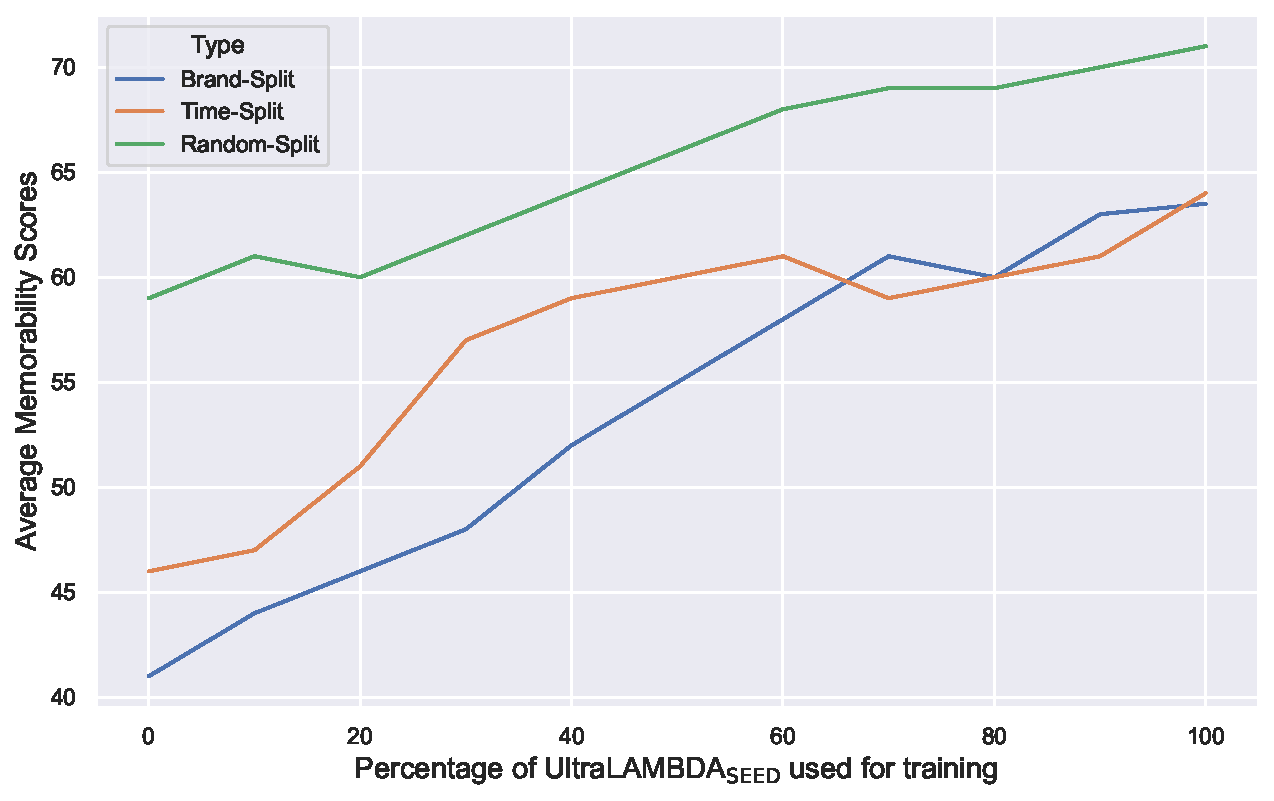
\includegraphics[width=0.45\textwidth]{images/henry/memorability.pdf}
%     \caption{Caption}
%     \label{fig:synthetic-data-vs-memorability-score}
% \end{subfigure}
% \begin{subfigure}
%     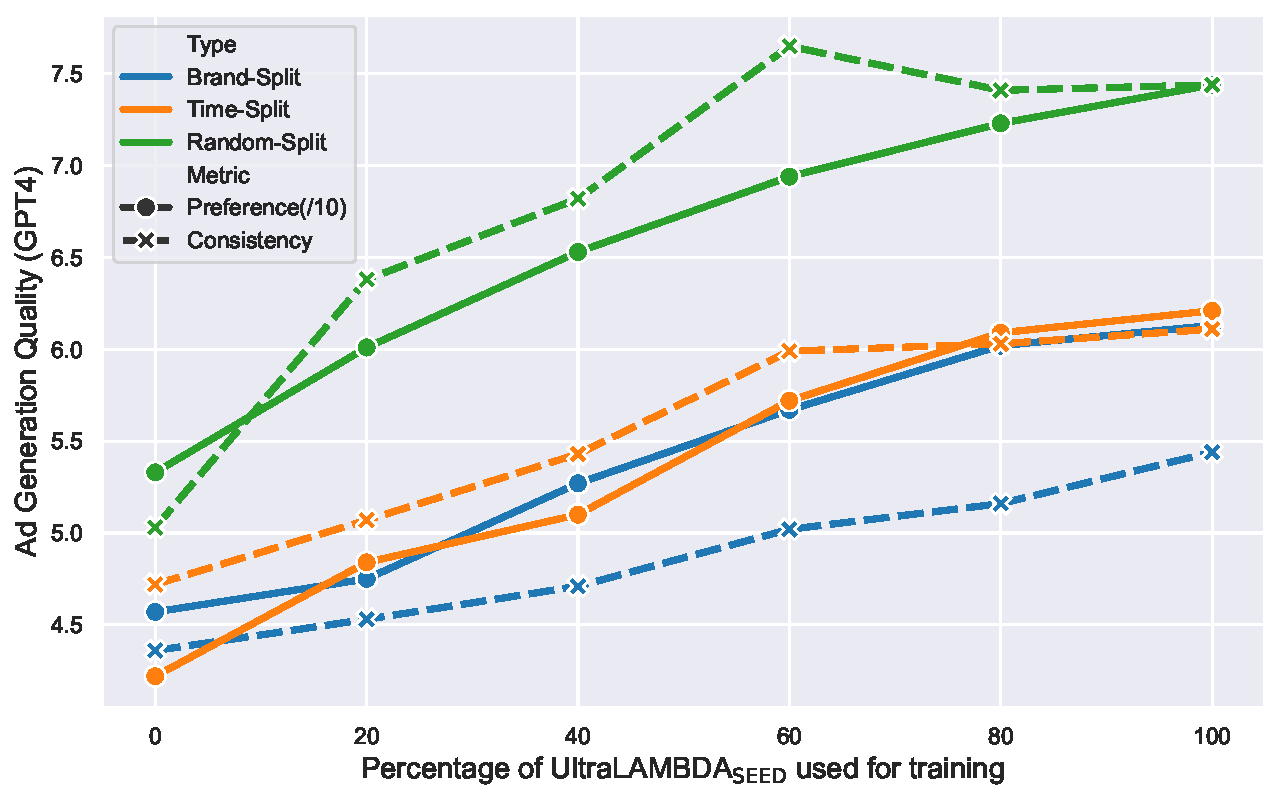
\includegraphics[width=0.45\textwidth]{images/henry/adquality.pdf}
%     \caption{Caption}
%     \label{fig:synthetic-data-vs-adquality}
% \end{subfigure}
% \end{figure*}



\subsection{Perplexity evaluation}
\label{sec:Perplexity evaluation}
A common approach to measuring language modeling performance on some data distribution $D$ is to measure \textit{perplexity}, which is defined as the exponential of the average negative loglikelihood per token \cite{perplexityjelinek, brown1992estimate,biderman2024lessons}, that is:
\begin{equation}
PPL = \exp\left(\frac{-1}{\sum_{j=1}^{|D|}N_j}\sum_{j=1}^{|D|}\sum_{i=1}^{N_j}\log P(y_{j_i}|y_{j_1}, \dots, y_{j_{i-1}})\right),
\end{equation}\label{eqn:ppl} where $|D|$ is the number of documents in the dataset, $y_j$ is the $j$-th document in $D$, $N_j$ is the total number of tokens in $y_j$, and $y_{j_i}$ represents the $i$-th token of $y_j$.

To calculate perplexity on a selected dataset $D$, each dataset document $y$ is tokenized and fed into a language model (following the procedure described below) via computing $\log P(y|x)$, where $x$ is set to either the empty string or a beginning-of-text token. Thus, given $\log P(y)$, for each document $y \in D$ we can sum up the per-document loglikelihoods and divide by the number of total dataset tokens.  



Given our language model, we aim to compute the conditional (log) probability (or ``loglikelihood'') of a target string $y$ conditioned on input $x$, denoted as $\log P(y|x)$. This can be performed in a single LM call.

Let $x = x_0, x_1, ..., x_{n-1}$ be an input sequence of $n$ tokens and $y = y_{0}, y_{1}, ..., y_{m-1}$ be the target sequence of $m$ tokens, where $x_i$ and $y_i$ represent individual tokens. To compute $\log P(y|x)$, we follow these steps:

\begin{enumerate}
    \item Concatenate $x$ and $y$ to form a new sequence, but discard the final token $y_{m-1}$. The resulting sequence is $x_0, x_1, ..., x_{n-1}, y_{0}, y_{1}, ..., y_{m-2}$.
    \item Pass this concatenated sequence through the language model to obtain logits $l$ of shape $(n + m - 1, |V|)$, where $|V|$ is the size of the vocabulary. The last $m$ positions in these logits correspond to the predicted probability distributions for the target tokens $y_0$ to $y_{m-1}$, conditioned on the input $x$ and the preceding target tokens.
    \item Apply a log-softmax function to the last $m$ logits to obtain log probabilities for the completion tokens only.
    \item Calculate the conditional loglikelihood of the target string $y$ given the input $x$ by summing the log probabilities of each target token:
    \begin{equation} \label{eqn:logp}
    \log P(y|x) = \sum_{i=0}^{m-1} \log p(y_{i}|x, y_0, ..., y_{i-1}) = \sum_{i=0}^{m-1} l(n +i, y_i),
    \end{equation} where $\log p(y_i|x, y_0, ..., y_{i-1})$ is the log probability of the $i$-th target token conditioned on the full input $x$ and the preceding target tokens. (and where $x, y_0,... y_{-1}$ denotes conditioning on only $x$.)
\end{enumerate}



We follow the above procedure to calculate perplexity over three equally divided parts of the dataset, \textit{i.e.}, 33-percentile cuts where samples are ranked as per their memorability values. The lower the perplexity of an LLM over a category of samples, the better it is at generating those samples. Therefore, for example, if an LLM has a lower perplexity over high memorable samples, it is easier for it to generate highly memorable samples than lower memorable ones.


%%%%%%%%%%%%%%%%%%%%%%%%%%%%%%%%%%%%%%%%%%%%%%%%%%%%%%%%%%%%%%%%%%%%%
%%%%%%%%%%%%%%%%%%%%%%%%%%%%%%%%%%%%%%%%%%%%%%%%%%%%%%%%%%%%%%%%%%%%%

\subsection{Annotation Protocol and Participant Details for the LTM Study}
Figure~\ref{fig:study protocol} shows a visualization of the annotation protocol we followed.




\begin{landscape}
    
\begin{figure*}[!h]
    \centering
    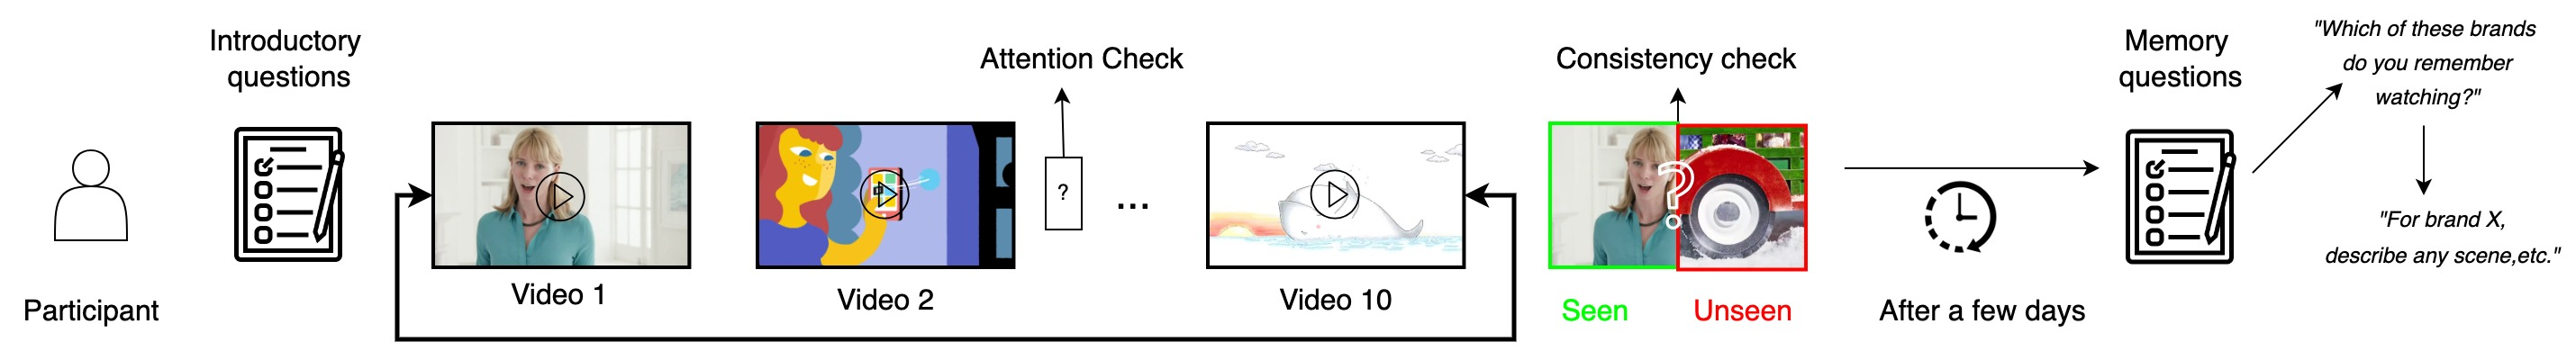
\includegraphics[width=1.5\textwidth]{images/Content-Memorability-final.jpg}
    \caption{The study protocol we followed for our long term memorability human study. All the previous works follow a game-like annotation protocol, where the study participants compete with each other to get best memorability scores and a participant is excluded from the study if their annotations fall below a certain threshold. We follow a more natural way in which participants fill an initial questionnaire, then watch 10 ads with attention checks on day 1 and in subsequent days, receive a form asking them to fill in what do they remember seeing. Further, using Stable Diffusion, we also ask them to recreate the scenes they remember.}
    \label{fig:study protocol}
\end{figure*}
\end{landscape}


The participants in the study were students who were offered optional course credit and freebies like eatables and a chance to see research and know their memorability scores. The participation was voluntary. The students were shown a protocol of the study and were required to sign the IRB approval, which was prominently displayed. The approval contained details about what kind of data was being collected and how the data would be used. The data collection protocol was approved by the IRB of the participating institution. The aggregate statistics were reported to each candidate after completing the study. Three emails were sent to take-home participants; if they didn't reply within the given time frame, their data was discarded from the experiment. 


The participants were primarily graduate and undergraduate students. The participants are from two universities spread across two locations in India. The participants are bilingual and speak a variety of languages, including English. The age range is from 16 to 35 years, and all genders/sexes are encouraged. We saw a roughly 30-70 distribution of females to males. 


\subsubsection{Memorability Questionnaire}
\label{sec:Memorability Questionnaire}
This section contains the questions we asked before the study, the attention check questions that were asked during the study, and finally, the recognition questions to check which brands were remembered.


\paragraph{Introductory Questionnaire (to be filled before the study starts)}

\begin{enumerate}
    \item I remember seeing ads for the following brands this year:
    \begin{itemize}
        \item List 15 randomly selected from the list of brands that we have
    \end{itemize}
    
    \item I remember using products of the following brands this year:
    \begin{itemize}
        \item List 15 randomly selected from the list of brands that we have (non-intersecting list from above)
    \end{itemize}
    
    \item Have you installed any Ad Blocking software in your browser(s)?
    \begin{itemize}
        \item[a.] Yes
        \item[b.] No
    \end{itemize}
    
    \item Do you use a Youtube subscription?
    \begin{itemize}
        \item[a.] Yes
        \item[b.] No
    \end{itemize}
    
    \item Approximately how much percentage of time do you spend on Youtube mobile vs Youtube web?
    \begin{itemize}
        \item $<$10\% on mobile
        \item $>$10\% but $<$30\% on mobile
        \item $>$30\% but $<$70\% on mobile
        \item $>$70\% on mobile
    \end{itemize}
    
    \item How do you apprise yourself of the latest products and brands? (Multi correct)
    \begin{itemize}
        \item Primarily friends and family
        \item Amazon, Flipkart or any other e-commerce stores
        \item Television and OTT Platform Ads (like Youtube, Netflix, Hotstar, etc)
        \item Email Ads
        \item Store Visits
        \item Website Ads
        \item I primarily search for products
    \end{itemize}
    \end{enumerate}
    
    
\paragraph{Checks (to be answered during the experiment)}
    \begin{enumerate}
        \item \textbf{Attention check}: A factual question like, What is the capital of India? (Asked randomly between videos, needs to be answered in $<$10s)
        \begin{itemize}
            \item[a.] Kanpur
            \item[b.] Delhi
            \item[c.] Goa
            \item[d.] Mumbai
        \end{itemize}
        \item \textbf{Consistency Check}:  Do you remember watching this video in this experiment (Asked after showing the 11th video)
    \begin{itemize}
        \item[a.] Yes
        \item[b.] No
    \end{itemize}
    \end{enumerate}

\paragraph{Recognition Questions (asked after a few days after watching the videos)}
\begin{enumerate}
    \item In the study, I remember seeing Ads of the following brands:
    \begin{itemize}
        \item (Randomly selected list of 20 brands which contains the brands shown to the participant)
        \item \{For each brand in the list which the participant has selected\}
    \end{itemize}
    
    \item Brand: X (already filled in)
    \begin{itemize}
        \item For the \{brand\} ad, I remember seeing the following (Write Scene Descriptions, feel free to write any scenes, music, characters, emotions, objects you remember seeing):
    \end{itemize}
\end{enumerate}





\subsection{Collection of all the Prompts used in the Paper}

\subsubsection{GPT-4 Prompts}
\begin{lstlisting}[caption={GPT-4 Prompt to calculate preference between Real Ad (A) and Generated Ad (B)},frame=single,breaklines=true,basicstyle=\tiny, label={lst:ad-quality-preference-prompt}]
As a seasoned marketer, evaluate the effectiveness of the following two ads using a comprehensive set of metrics:

Creativity and Innovation: Originality and uniqueness in conveying the message. Use of unexpected ideas or elements that grab viewers' attention.

Emotional Connection: Ability to evoke strong, relevant emotions in the target audience. Establishing a connection between the brand and the viewers' emotions.

Storytelling: Crafting a compelling narrative that engages and retains the audience. Creating a memorable experience through a coherent and impactful story.

Visual Appeal: Use of strong visual elements, such as striking visuals, colors, and graphics. Ensuring that the visual elements align with the overall message and brand image.

Brand Alignment: How well the ad aligns with the values, mission, and personality of the brand. Consistency with the brand's visual identity, tone, and messaging. The ad's ability to leave a lasting impression on viewers regarding the brand. Incorporating brand elements that make it easy for the audience to remember and recognize.

Target Demographics: Relevance of the ad content and message to the target audience. Appropriateness of visuals, language, and themes for the specific demographic group.

Based on these criteria, analyze and determine which of the two ads is more effective. I will provide you with the Voiceover, followed by their scene-by-scene descriptions, including the emotions shown in the scene, the text, objects, colors, and style of the image.

Ad (A): {Verbalization for Ad (A)}

Ad (B): {Verbalization for Ad (B)}

Give me your answer in a json format, with the following keys:
- ad_a_score: Score between 0 and 10 for Ad A
- ad_b_score Score between 0 and 10 for Ad B
- winner The winner of the two ads
- reason line separated Reasons for the winner in not more than 3 lines
\end{lstlisting}



\begin{lstlisting}[caption={GPT-4 Prompt to measure consistency of an Ad},frame=single,breaklines=true,basicstyle=\tiny, label={lst:ad-quality-consistency-prompt}]
You are now a seasoned marketer that judges the consistency of an advertisement well. The consistency of an Ad can be determied by a few metrics (in no particular order) such as:
1. Does the voiceover match with the Scenes in the Ad?
2. Do the scene description make a good story?
3. Are the emotions depicted in the scenes consistent with the overall ad?
4. Does the ad represent the product and the brand well?

Rate the consistency of the following ad out of 10. Give me the rating only and nothing else, or you will be penalized.
{Advertisement Description}
\end{lstlisting}




\begin{lstlisting}[caption={GPT-4 Prompt to generate ad verbalization with In-Context-Learning (ICL)},frame=single,breaklines=true,basicstyle=\tiny, label={lst:ad-gen-prompt}]
You are now a seasoned marketer that creates memorable ads given its duration, brand and title.
Your output should follow the writing style of the input exactly. For example, each scene should look like:
The scene shows {}. The foreground colors of the scene are {}, and the background colors are {}. The dominant tone of the scene is {}. The photography style of the scene is {}. The scene has {} visual complexity. The emotions shown in the scene are {}.  This scene is categorized by the tags {}. 
You are only supposed to fill in the {}

Generate the detailed description of a {DURATION_AD1} second memorable advertisement titled "{TITLE_AD1}" for the brand {BRAND_AD1}
Generate the detailed description of a {DURATION_AD2} second memorable advertisement titled "{TITLE_AD2}" for the brand {BRAND_AD2}
...
Generate the detailed description of a {DURATION_AD5} second memorable advertisement titled "{TITLE_AD5}" for the brand {BRAND_AD5}
Generate the detailed description of a {DURATION_TARGET} second memorable advertisement titled "{TITLE_TARGET}" for the brand {BRAND_TARGET}
\end{lstlisting}



\subsubsection{Henry Prompts}
\label{sec:Henry-prompts}
Given below are the verbalization templates we use to teach Henry and Henry-SEED behavior simulation and content simulation tasks:



\begin{lstlisting}[caption={Verbalization pattern to predict memorability given advertisement. The same template is used to prompt GPT-3.5, GPT-4, Henry, Henry-Oracle, and Henry-SEED. Note that video tokens are optional.},frame=single,breaklines=true,basicstyle=\small\ttfamily,label={listing:memorability-prediction-verbalization-format}]
Students are shown ads and their memorability is tested after 1 to 3 days. For the given ad: 
<video> .. </video> 
They watch a 15 second advertisement for Chanel. 
The title of the advertisement is " Comes in Red for a Limited Edition CHANEL Fragrance". 
The ad is shot in landscape orientation, at a medium pace.
The audio in the ad says: Number 5. Limited Edition. Chanel. 
Following are the descriptions of each scene: 
    Scene 1: 
        The scene shows a red bottle of perfume that is on a dark surface.
        The foreground colors of the scene are Black, and the background colors are Dark_Brown,Maroon,Black,Gray.
        The dominant tone of the scene is neutral.
        The photography style of the scene is product. 
        The scene has Low visual complexity.
        The emotions shown in the scene are gift, romantic, celebration. 
        This scene is categorized by the tags bottle, man, perfume, red, woman.
        The text shown in the scene is 'N5', 'CHANEL', 'PARIS', 'PARFUM' 
        ....
What would be the memorability score of this video?

Output: 71
\end{lstlisting}
%\end{verbatim}



\begin{comment}
        
    \begin{lstlisting}[caption={Henry prompt to evaluate the memorability},frame=single,breaklines=true,basicstyle=\tiny,]
    Students are shown ads and their memorability is tested after 1 to 3 days. For the given ad:
    {Advertisement Description}
    Return the long term memorability score of the video on a scale of 00 to 99 without any explanation.
    \end{lstlisting}
\end{comment}


\begin{lstlisting}[caption={Henry Prompt to generate ad verbalization used to train and evaluate Henry-SEED},frame=single,breaklines=true,basicstyle=\tiny,label={listing:advertisement-generation-prompt-Henry-SEED}]
Generate the detailed description of a {DURATION_TARGET} second memorable advertisement titled "{TITLE_TARGET}" for the brand {BRAND_TARGET}
\end{lstlisting}



\subsubsection{Mistral prompt for filtering marketing ads}
\label{lst:msitral-filter-prompt}
\begin{lstlisting}[caption={Mistral Prompt for Ad Filtering},label={listing:Mistral Prompt for Ad Filtering},frame=single,breaklines=true,basicstyle=\tiny,]
"Based on the topic_tags_vocab = {'politics': 'The art and science of governing societies and making decisions that affect collective interests.', 'marketing': 'The process of promoting, selling, and distributing products or services to consumers, often involving market research, advertising, and branding strategies.'} provided, please identify the top most relevant topic tag from the topic_tags_vocab keys that represent the following advertisement based on content and page_name. Please use only the most relevant tag and make sure to choose from provided topic tags only. Do not include any other tags not mentioned in the prompt.Answer with the most relevant topic tag only. The advertisement is posted by the page Donald J. Trump and has the following content : ['President Trump is coming to town! Get your free tickets now >>>']. Answer in only politics or marketing."

cleaned_text = "The advertisement is posted by the page {page_name} and has the following content : {page_content}"
\end{lstlisting}

\subsection{Computing Infrastructure and Hyperparameters}
\subsubsection{Modeling Memorability}
\label{sec:experimental-details}
All the experiments were conducted on 8x40 A100 instances. All experiments were performed leveraging DeepSpeed ZeRO stage-3 with cpu offload \cite{ren2021zero,rasley2020deepspeed,rajbhandari2020zero} and Flash-attention \cite{dao2022flashattention} with gradient-checkpointing \cite{chen2016training} at bf16 precision. We use AdamW as the optimizer (with fused gelu), the learning rate was kept 2e-5 for all experiments. The maximum context length for image-only datasets is 500, including public video datasets is 800 and including our dataset is 2048. The corresponding batch sizes are 32,16,8. The gradient accumulation is set to 1 and weight decay is disabled. The warmup steps are set to 20 and residual dropout was kept at 0.25. We train all models for two epochs, but use the checkpoint with best validation spearman correlation.

For all experiments, where we combine datasets, we use a custom sampler to account for dataset imbalance, that ensures a maximum proportion of the dataset in an epoch, here are the maximum proportions. For validation we take 5\% of each dataset.
We use the provided test splits for public datasets and we use a 15\% test split for our dataset

\paragraph{Images}
\begin{enumerate}
    \item \textbf{Lamem} 50\%
    \item \textbf{Memcat} 100\%
    \item \textbf{SUN} 100\%
\end{enumerate}

\subsubsection{Videos}
\begin{enumerate}
    \item \textbf{VideoMem} 75\%
    \item \textbf{Memento} 75\%
    \item \textbf{AdsData} 100\%
    \item \textbf{MediaEval} 100\%
\end{enumerate}

\subsubsection{Generating Memorable Ads}
All the experiments were conducted on 8x80 A100 instances. All experiments were performed leveraging DeepSpeed ZeRO stage-2, Flash Attention and Gradient-Checkpointing.
$\alpha=0.001$, awac\_scale$=1$, $\gamma=0.99$, $\beta=0$ cql\_scale$=0.1$
\subsubsection{Inference hyperparameters}
$\beta=4$, temperature$=0.8$, steps\_for\_target\_sync 10, 
$\tau=0.7$, two\_qs: True, lr=1e-5


\subsection{License and Terms of Release}
LAMBDA and UltraLAMBDA are sourced from brand videos from YouTube, Facebook Ads, and CommonCrawl. The dataset annotations and video links contained in LAMBDA and UltraLAMBDA will be released under CC BY-NC 4.0 license. The videos themselves are released as per their creators' licenses. The videos or the released data do not contain or disclose any identities of their annotators or any specific persons. Since it is handcrafted, LAMBDA makes sure that none of the videos are offensive; UltraLAMBDA being sourced from the internet is noisier. While the videos themselves originate from brands, the content of some brands may seem offensive to certain people. 

We used Llama, GMHRA, ViT, EVA-CLIP, and Qformer models in accordance with their licenses to train Henry.  





\begin{comment}
\setcounter{section}{0} % Restart section numbering
\vspace{-10mm}
\section{Rebuttal}

Thank you for giving a thorough read to the paper! \textcolor{pink}{\faSmile} Below, we try our best to answer the questions asked in your reviews:
%How did you determine the factors that contribute to long-term memorability in advertisements? Did you conduct any preliminary studies or experiments?

\noindent \textcolor{red}{\textbf{Reviewer-\#1:}}  \textcolor{blue}{Factors contributing to long-term memorability:} We use a mix of experimentation and litt sources to determine contributing factors. In particular, the following sources motivated us: content factors:\{speech-ratio \cite{bellman2021can}, emotion \cite{putrevu2004consumer,mai2009emotions}, length \cite{newstead2010cost,varan2020effects}\}, interaction factors:\{order \cite{li2010primacy}\}, customer behavior:\{brand relevance \cite{newstead2010cost,schmidt2015advertising}\}. Further, since we conducted the overall study in four legs, we observed the effect of these variables on memorability. For e.g., in the first leg we observe that contrary to previous studies, the order of videos had little effect, and we confirmed this in the subsequent legs.

\noindent \textcolor{blue}{Criteria to select subjects:} Motivated by the general use case of advertising, we had broad-based criteria for subject selection (of any student in our universities). We consider any subject who watched all videos and completed their annotations in a set time (5 days). %On the other hand, study videos had to be carefully collected since they would have to be consistent with the goal and should not be completely culture and language-agnostic, otherwise, they would have led to subjects not having any clue about the products or advertising.  
This enabled us to reach a broad audience of 1203 subjects. After the submission, we extended our study to 516 more subjects, making it 1719 subjects in total.


\noindent \textcolor{blue}{Reliability and Validity Metrics:} Similar to previous works \cite{cohendet2019videomem}, we measured consistency scores for our dataset. Table-3 reports the consistency for all datasets. To evaluate consistency, the subject pool is split into two independent halves and quantified how well image scores measured on the first half of the subjects matched image scores measured on the second half. With the data reported in the paper, the consistency is 0.55, with the new data collected post-submission, it is 0.61.


\noindent \textcolor{blue}{Measuring brand recognition and ad recall:} Brand recognition is measured (Sec.2.2) by presenting subjects with 20 options where they have to select which brands they remember from the videos they watched. Ad recall (since is a type of recall) is open-ended, where subjects are asked to describe what they remember about ads of the recognized brands. We use recognition to train Sharingan. We haven't used recall in this work.

\noindent \textcolor{blue}{Study Generalizability, Diversity of industry \& brands:} Yes, we cover 2205 videos with 276 brands covering 113 industries (Sec.2.1) with the time diversity. The videos are diverse also in terms of scene velocities, human presence, animations, visual and audio branding, emotions, scene complexity.

\noindent \textcolor{blue}{Rationale behind using a combination of visual knowledge and world knowledge:} Understanding ads needs both visual knowledge to understand the moving graphics and world knowledge to understand the product, brand, and its connection with use-cases. Further, we have shown in Table 5 the importance of each knowledge type (enhanced in Table 1 attached).




We have one more request; in Q 5 (novel resources), you mentioned that we don't contribute any resources. Can you please correct it? Since we are releasing the largest LTM dataset.




\noindent \textcolor{red}{\textbf{Reviewer-\#3:}} \textcolor{blue}{Evaluation of each component of the architecture:} We evaluate most components of the architecture in Table-5. In the limited rebuttal time, we also extended the ablation across all the architectural choices. We are attaching the results with this rebuttal in Table-1.

\noindent \textcolor{blue}{Few related works in Table-3:} We have covered all the state-of-the-art results in the literature. We can report other underperforming methods as well in the camera-ready.

\noindent \textcolor{blue}{Fig-3 layout:} We acknowledge this and plan to improve it.

% \begin{table}[!th]
% \vspace{-8mm}
% \centering
% \resizebox{0.45\textwidth}{!}{%
% \begin{tabular}{llllllll}
% \hline
% & \textbf{Train/Inference}
% & \textbf{Lamem} & \textbf{Memcat} & \textbf{SUN}  & \textbf{VideoMem} & \textbf{Memento10k} & \textbf{Our study} 
% \\ \hline
% \makecell{Vision only\\(Eva-CLIP+\\Linear Layer)} & train & 0.15  & 0.14   & 0.12 & -        & -         & -         \\
% \makecell{Vision only\\(Eva-CLIP+\\GMHRA+QFormer+\\Linear Layer)} & train & 0.20  & 0.17   & 0.15 & 0.17     & 0.21     & 0.11      \\
% Verbalization only& train & 0.51  & 0.53   & 0.53 & 0.42     & 0.54    & 0.39      \\
% vision+verb-emotion& train & 0.68  & 0.76   & 0.71 & 0.54     & 0.67    & 0.47      \\ 
% vision+verb-asr& train  &-       &-        &-       & -       &-         & 0.45         \\
% \makecell{Sharingan} &train & 0.72  & 0.79   & 0.76 & 0.60     & 0.72    & 0.52      \\
% Sharingan-emotion&inference &0.69       &0.75        &0.75      & 0.58       &0.70         & 0.49         \\
% Sharingan-asr&inference &-       &-        &-       & -       &-         & 0.46         \\
% Sharingan vision only&inference &0.16       & 0.14       &0.13       &0.12        &0.17         &0.08  \\
% Sharingan-asr-emotion&inference &-       &-        &-       & -       &-         &0.42         \\
% Sharingan-object tags&inference &0.70       &0.77        &0.75       &0.57       &0.70         &0.48         \\
% Sharingan-colors&inference &0.69       &0.77        &0.73      &0.55       &0.68         &0.49         \\
% Sharingan-aesthetics&inference &0.70       &0.76        &0.75       &0.60       &0.70         &0.50         \\\hline\vspace{-3mm}
% \end{tabular}%
% }
% \caption{\vspace{-2mm} \footnotesize Ablation across architectural choices.\vspace{-5mm}}
% \label{table:architecture-ablation}
% \end{table}


    

\begin{table}[!th]
\vspace{-5mm}
\centering
\resizebox{0.5\textwidth}{!}{%
\begin{tabular}{lllllll}
\hline

& \textbf{Lamem} & \textbf{Memcat} & \textbf{SUN}  & \textbf{VideoMem} & \textbf{Memento10k} & \textbf{Our study} 
\\ \hline
\makecell{Sharingan} & 0.72  & 0.79   & 0.76 & 0.60     & 0.72    & 0.52      \\
Sharingan-emotion &0.69       &0.75        &0.75      & 0.58       &0.70         & 0.49         \\
Sharingan-asr &-       &-        &-       & -       &-         & 0.46         \\
Sharingan vision only &0.16       & 0.14       &0.13       &0.12        &0.17         &0.08  \\
Sharingan-asr-emotion &-       &-        &-       & -       &-         &0.42         \\
Sharingan-object tags &0.70       &0.77        &0.75       &0.57       &0.70         &0.48         \\
Sharingan-colors &0.69       &0.77        &0.73      &0.55       &0.68         &0.49         \\
Sharingan-aesthetics &0.70       &0.76        &0.75       &0.60       &0.70         &0.50         \\\hline\vspace{-3mm}
\end{tabular}%
}
\caption{\footnotesize Ablation across architectural choices. ``-'' denotes non-speech dataset\vspace{-5mm}}
\label{table:architecture-ablation}
\end{table}

\noindent \textcolor{blue}{Training Details:}
Instruction format - We have given the verbalization template in Listing-1 in the Appendix. The ``00-to-99'' is also given in the same template. It denotes the percentage of times the brand was recognized whenever it was presented to the subjects. It is used to train the Sharingan model (Fig.3). We ask the model to output it in 00-to-99 format. We also tried ``0-to-9'' and ``0-to-99'' but ``00-to-99'' gave the best results.


\noindent \textcolor{red}{\textbf{Reviewer-\#6:}} \textcolor{blue}{Description of the reported metric:} Similar to previous works \cite{cohendet2019videomem}, we use Spearman rank correlation between the memorability ranking produced by the ground-truth memorability scores versus the predicted scores

\noindent \textcolor{blue}{Contribution of semantic categories:} We evaluate most components of the architecture in Tables-5 and 6. In the limited rebuttal time, we also extended the ablation across all the architectural choices. We are attaching the results here in Table-1.


\noindent \textcolor{blue}{Missing values in Table-3:} In Table-3, we have reported the state-of-the-art results reported in the literature. The missing values indicate wherever the results are unavailable; for instance, on our dataset literature SOTA is unavailable, similarly ViTMem has not reported scores on MediaEval. 


\noindent \textcolor{red}{\textbf{Reviewer-\#7:}} \textcolor{blue}{Model Limitations:} On our dataset we observe lower performance on longer verbalizations ($>$1500 tokens). Moreover, the model is slightly inaccurate for ads with substantial music. We will cover this in the final version better.

% tends to have poorer performance in cases when the verbalization gets too long, for eg: when the video is longer or when the ASR/OCR extracted is lengthy. The model can also be slightly inaccurate in music-heavy videos.

\noindent \textcolor{blue}{Advantages of the new memorability measurement protocol:} All the previous studies were measured with a competitive game where they subjects competed to recognize as many images as possible and the game ended for people who couldn't recognize beyond a certain threshold. These conditions are understandable for short-term memorability settings. However, our protocol is fine-tuned for long-term memorability settings. Sec-2.2 covers the annotation protocol, where we keep the settings as natural as possible. The subjects first answer some introductory questions, then view the videos, and then after a few days answer the memorability questionnaire. 

\noindent \textcolor{blue}{Interpretation of missing values in Table-3:} 
In Table-3, we have reported the state-of-the-art results reported in the literature. The missing values indicate wherever the results are unavailable, for instance, on our dataset literature SOTA is unavailable, similarly ViTMem has not reported scores on MediaEval. 


\noindent \textcolor{blue}{Dataset Name:} That's a good suggestion. We will name the dataset and release it.


\noindent \textcolor{red}{\textbf{Reviewer-\#4:}} \textcolor{blue}{Novelty:} (1)~first large-scale human study for LTM covering 1800 subjects, 2205 ads, 276 brands, (2)~novel architecture achieving SOTA results on 8 datasets over both images and videos, (3)~effect of various effects on LTM. 

\noindent \textcolor{blue}{Architecture:} To the best of our knowledge, no one has released this architecture where we combine various components to achieve SOTA results. The idea of leveraging visual perception models for memorability modeling is also novel. The overall architecture is Sharingan (not just Llama component). We will clarify this in camera-ready version better. In Q5 you have answered no, can you please make it yes?

1. Number of interactions
\end{comment}



\subsection{Limitations and Potential Risks}
In this paper, we try to fill a gap in the existing literature about long-term memorability modeling and datasets. Therefore, we conduct the first study for that purpose. While doing that, we have made initial efforts starting with the English language advertisements. Future work would be needed to address other languages. Further, given the limitations of the study, we conducted it in an academic environment with a student population consisting of undergraduate and graduate student volunteers. We will expand the scope to a wider audience in the future work. We trained a model, Henry, on the collected dataset, showing good performance on all literature datasets. However, since the literature datasets are all English-based and deal with a majorly uniform population, the training will be scaled to more languages and population types in future work. We also observed a decrease in performance for brands not seen during the training and for videos with longer verbalizations exceeding 1500 tokens. Additionally, the model exhibits a slight inaccuracy when advertisements have significant musical content. In our opinion, the model does not pose any potential risk or harm besides the limitations mentioned here. We also conduct a review of the generated ads through experts and non-expert annotators. Both experts and non-expert annotators preferred Henry-SEED generated ads 3/5 times.







\FloatBarrier
%%%%%%%%%%%%%%%%%%%%%%%%%%%%%%%%%%%%%%%%%%%%%%
%%%%%%%%%%%%%%%%%%%%%%%%%%%%%%%%%%%%%%%%%%%%%%
%%%%%%%%%%%%%%%%%%%%%%%%%%%%%%%%%%%%%%%%%%%%%%
%%%%%%%%%%%%%%%%%%%%%%%%%%%%%%%%%%%%%%%%%%%%%%
%%%%%%%%%%%%%%%%%%%%%%%%%%%%%%%%%%%%%%%%%%%%%%

\section{Measuring And Improving Engagement Of Text-to-Image Generation Models}
Recent advances in text-to-image generation have achieved impressive aesthetic quality, making these models usable for both personal and commercial purposes. However, in the fields of marketing and advertising, images are often created to be more engaging, as reflected in user behaviors such as increasing clicks, likes, and purchases, in addition to being aesthetically pleasing.
% created to drive specific user behaviors such as increasing clicks, likes, and purchases, in addition to being aesthetically pleasing. 
To this end, we introduce the challenge of optimizing the image generation process for improved viewer engagement. In order to study image engagement and utility in real-world marketing scenarios, we collect \textit{EngagingImageNet}, the first large-scale dataset of images, along with associated user engagement metrics. 
Further, we find that existing image evaluation metrics like aesthetics, CLIPScore, PickScore, ImageReward, \textit{etc.} are unable to capture viewer engagement.
To address the lack of reliable metrics for assessing image utility, we use the \textit{EngagingImageNet} dataset to train \textit{EngageNet}, an engagement-aware Vision Language Model (VLM) that predicts viewer engagement of images by leveraging contextual information about the tweet content, enterprise details, and posting time. %\textit{EngageNet} demonstrates superior performance in predicting image engagement, significantly surpassing much larger models like GPT-4V. 
We then explore methods to enhance the engagement of text-to-image models, making initial strides in this direction. These include conditioning image generation on improved prompts, supervised fine-tuning of stable diffusion on high-performing images, and reinforcement learning to align stable diffusion with \textit{EngageNet}-based reward signals, all of which lead to the generation of images with higher viewer engagement. Finally, we propose the \textit{Engagement Arena}, to benchmark text-to-image models based on their ability to generate engaging images, using \textit{EngageNet} as the evaluator, thereby encouraging the research community to measure further advances in the engagement of text-to-image modeling. These contributions provide a new pathway for advancing utility-driven image generation, with significant implications for the commercial application of image generation.



\subsection{Introduction}
 \label{sec:intro}
%  \cy{High-level comment: Currently it is too long, most of the figures, tables can be shrink by using libraries such as scalebox and wrapfig, etc. Also, some details in the method part can be moved to the appendix, e.g., Section 4.3}

% \cy{Introduction should be shrink to at most 2 pages.}
 
 % motivation - answering why is this work necessary
 % 1. Measuring engagement, 2. New metric, new dataset 3. Initial attempts at solving it, 4. Introducing new problem
 Machine learning models that interact with humans are built as a means to achieve an end, and performance metrics in their respective fields reflect how effectively these models meet the ends. For instance, recommendation systems are optimized to capture maximum viewer interest and the key performance metrics tracked by the research community are clickthrough rates and the number and ranking of relevant documents recommended out of the total document set \cite{bobadilla2013recommender}. Similarly, chat assistants are optimized for being helpful, and the commonly tracked metrics are the scores of responses preferred by humans \cite{ouyang2022training,stiennon2020learning}. In the case of image generation, industries such as e-commerce, fashion, education, and advertising aim to optimize user-focused outcomes like clicks, purchases, retention, and user engagement. However, the metrics used by the image generation research community often emphasize \textit{aesthetic appeal} \cite{xu2024imagereward,kirstain2023pick,black2023training} and \textit{realism} \cite{dhariwal2021diffusion,saharia2022photorealistic,ho2020denoising,rombach2022high} factors that crucial for image acceptability but not necessarily aligned with the ultimate goals of viewer engagement. 
 
 %search and retrieval are optimized to get relevant documents to a user's query \textit{faster} \cite{menick2022teaching}, game-play is optimized for increasing complexity to keep humans \textit{engaged} \cite{nadiger2019federated}, chat-engines are optimized for being \textit{helpful} \cite{ouyang2022training}, and summarization systems are optimized to keep those sentences in the summary which humans consider as important \cite{stiennon2020learning}. However, today, image generation is optimized with the twin goals of looking better (aesthetics) and matching reality. On the other hand, in the real world, images are created as a means to an end. For example, images in marketing are used to engage viewers and gather more clicks and purchases.   
 
 %In a world where more and more content is being automatically generated, we ask the question, how do we optimize images to get the desired behavior from the receiver? Answering this question translates to direct financial, political, and social gains to advertisers, political parties, and governments, respectively. %For example, although the U.S. government has allocated billions of dollars towards vaccination-related initiatives by the Center for Disease Control and Prevention (CDC) \cite{sekar2021domestic}, and the US Department of Health and Human Services has invested an unprecedented \$250 million into campaigns targeting the coronavirus \cite{PRWeek_DefeatDespairCOVID19}, vaccine hesitancy persists alongside low vaccination rates across various demographic groups \cite{dror2020vaccine,sallam2021covid}. A system that can generate provably persuasive messages can potentially help break this vaccine hesitancy. Conversely, such systems can also be used to exert a harmful influence on societies, such as shaping political inclinations \cite{tappin2023quantifying}, amplifying the dissemination of misinformation \cite{lukito2020coordinating}, or encouraging ill-informed consumer choices \cite{boerman2017online}. 

 %\textbf{Lack of metrics and dataset to measure image persuasiveness:} Today, images are generated to be more real-looking  or aesthetical . Advances in fulfilling these objectives have brought image generation technology to a threshold such that it is being widely deployed in commercial applications. However, the utility of an image is \textit{better communication}. The images are, therefore, a means to an end. For instance, in the case of marketing, an image's utility is to bring in the desired \textbf{customer engagement} measured through metrics like clicks, likes, shares, and comments, ultimately leading to more sales and brand building. On the other hand, in text-to-image generation, there has been little progress on this front, with the most common metrics, FID \cite{heusel2017gans} and aesthetics \cite{schuhmann2022laion}, comparing the structural integrity and beauty of generated images, and 

 \begin{figure}[!t]
   \centering
   %\vspace*{-15pt}
   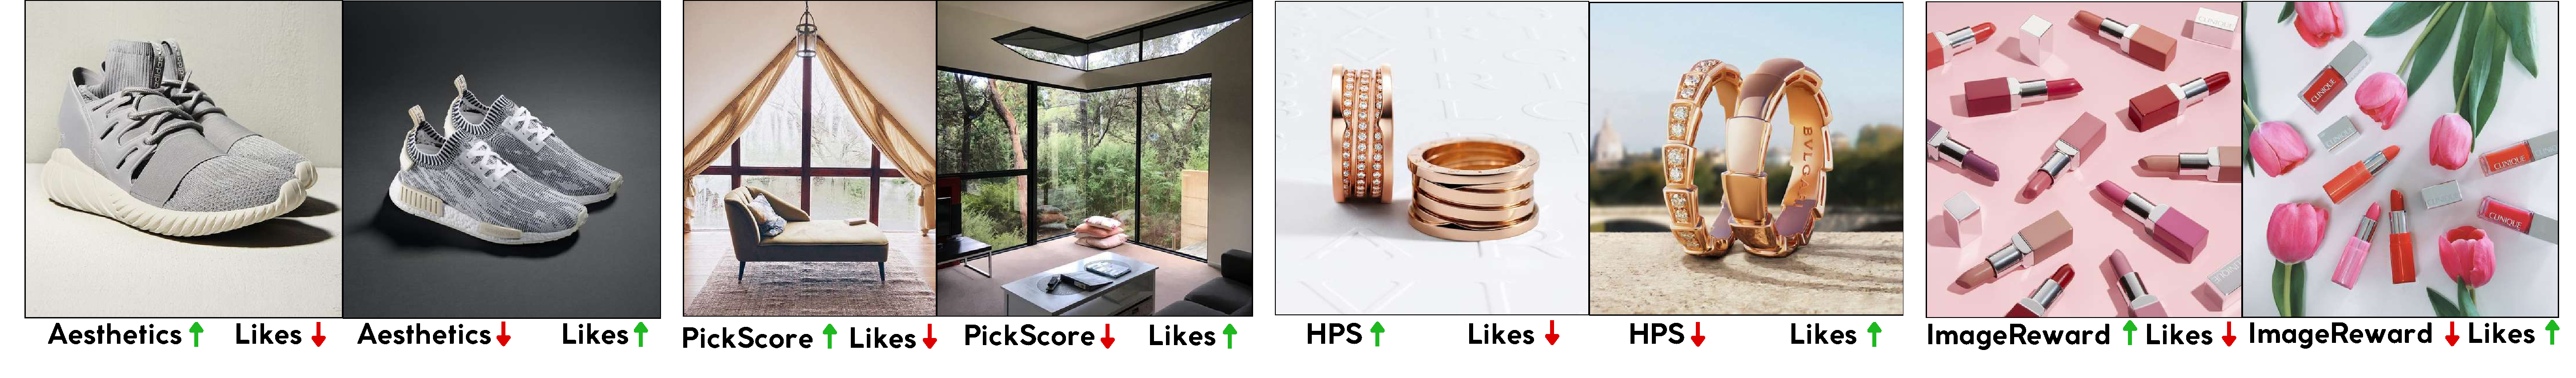
\includegraphics[width=\textwidth]{images/metric_non_alignment_compressed.pdf}
   %\vspace*{-10pt}
   \caption{Some images from the EngagingImageNet dataset. We constructed pairs of similar images posted within a 45 days interval by the same account. In each pair shown in the figure, the left image corresponds to lower likes and the right one received higher likes. However, existing image generation metrics like Aesthetics, PickScore, Human Preference Score, ImageReward, \textit{etc.}, exhibit image preference in the opposite direction as actual user engagement. 
   \label{fig:metric_non_alignment_with_engagement}}
   %\vspace*{-10pt}
 \end{figure}

 
 We find that popular image generation metrics such as Aesthetics \cite{schuhmann2022laion}, ImageReward \cite{xu2024imagereward}, Human Preference Score (HPS) \cite{Wu_2023_ICCV}, and CLIP-H \cite{radford2021learning} have a correlation ranging from 0.02-0.08 with user engagement measured by likes, roughly equal to random chance (Table~\ref{tab:EngageNet_kpi_prediction_results}). Fig.~\ref{fig:metric_non_alignment_with_engagement} illustrates this effect through some randomly picked high and low engagement image samples. Further, one may think that the preferences of image creators (\textit{e.g.}, in the form of upvotes on platforms like Pick-a-Pic \cite{kirstain2023pick} or Discord \cite{Wu_2023_ICCV}) are a good estimate of image-consumer engagement. However, we find that PickScore and HPS, the reward models trained on a large dataset of creator preferences, correlate 0.07 with user engagement. Therefore, there is a lack of reliable metrics capturing viewer engagement on images. 


 The lack of progress can largely be attributed to the absence of a large and open dataset of customer engagement metrics over images. The most common image generation datasets, MS-COCO \cite{lin2014microsoft} and LAION \cite{schuhmann2022laion}, contain no signals for user engagement. 
 %To fill this void, we collect a large-scale dataset of customer engagement in the form of likes over a wide variety of marketing tweets over a period of 17 years. 
 Therefore, to spur research in the direction of measurement and optimization of image generation for user engagement, we curate a large-scale dataset, \textbf{EngagingImageNet}. EngagingImageNet (\S\ref{sec:EngagingImageNet}) consists of 168 million tweets capturing 17 years of high-quality enterprise images for over ten thousand brand accounts and average user engagement of images in the form of likes\footnote{EngagingImageNet was collected using Twitter academic API over a period of several years.}. We release EngagingImageNet to serve as a starting point for measuring, benchmarking, and modeling large-scale engagement-optimized image generation. %We cover more details of the dataset in .
 
 
 
 
 \textbf{EngageNet as a scoring function to score engagement:} EnagingImageNet allows us to train a scoring function that estimates the user engagement on a particular generated image. We formulate this problem as simulating the engagement in the form of user likes over an image-containing tweet (\S\ref{sec:EngageNet}). We carry out visual instruction finetuning of LLaVA-1.5 13B \cite{liu2023visual} model to estimate the brand-normalized likes given the image along with contextual information that includes input account handle, image description, and time of the tweet. We find that the resulting scoring model, \textbf{EngageNet}, achieves a high correlation of 0.62 with actual user engagement. %We compare EngageNet's performance with state-of-the-art language models (GPT-3.5 \cite{ouyang2022training}, GPT-4V \cite{openai2023gpt4}), and observe that EngageNet strongly outperforms them despite being significantly smaller in size. Curiously, while in-context learning over GPT-3.5 and GPT-4V has been shown to work well in other domains \cite{min-etal-2022-rethinking}, it does not work in engagement-simulation (Table~\ref{tab:EngageNet_kpi_prediction_results}). 
 

 \textbf{Engagement Arena:} Next, leveraging EngageNet as a judge, on the lines of LMSYS arena \cite{zheng2024judging,chiang2024chatbotarenaopenplatform}, we propose \textbf{Engagement Arena}, an arena where we test the engagement of images generated by various image generation models for the same prompt. Using EngageNet's reward estimates, we compute Elo ratings of a number of popular open-source text-to-image generation models, including Stable Diffusion-3 \cite{esser2024scaling}, Flux.1-dev \cite{blackforestlabs2024}, Stable Diffusion-XL \cite{podell2023sdxl}, SDXL-DPO \cite{wallace2024diffusion}, PixArt-alpha \cite{chen2024pixartalpha}, Pixart-sigma \cite{chen2024pixart}, Stable Diffusion 2.1 \cite{rombach2022high}, \textit{etc}, and closed-source models like DALL.E-2 \cite{ramesh2022hierarchical}. Further, we encourage the research community to adopt Engagement Arena as a basis for measuring further advances in the engagement capabilities of text-to-image modeling and incorporating user engagement into the learning process. 
 
 %This problem can be formulated in two ways: (1)~\textbf{Behavior-simulation (BS)} where the reward model scores an image for the expected user engagement, and (2)~\textbf{Content-simulation (CS)} where the reward model measures the closeness of an image with a design specification designed to bring in maximal user engagement (Fig.~\ref{}). We train LLaMA-13B \cite{} to estimate the reward in both ways. 
 %Once trained, EngageNet can generate natural language descriptions of how an image conditioned on behavior should look like. Further, EngageNet's logits act as the simulator to test the effectiveness of an image in real-world settings (\S\ref{sec:Performance Aligning Stable Diffusion}). 
 %To design a model that can generate natural language descriptions of images based on their potential to elicit different effects, we design a large language model (LLM) that understands both images (content) and receiver behavior, such as likes and downloads. We call this model EngageNet. To train EngageNet, we present four types of behavior fine-tuning \cite{khandelwal2023large} (\S\ref{sec:EngageNet}, Listing~\ref{EngageNet:verbalization-1}-\ref{EngageNet:verbalization-4}) to train the model to predict image attributes for a given communicator, time, channel, topic, and intended behavior.
 
 
 %The next step in the evolution is to optimize the image generation with the goal of the image-maker. 
 
 
 
 
 %Images, in the form of messages like text, can be used as a means of communication. A receiver, upon receiving a (image-based) message from a sender, interacts with the message, thereby generating effects (analytics) such as likes, comments, shares, and purchases (Fig.~\ref{fig:factors-of-communication-eoig}). Just about every transaction involving an image can be formulated as a transaction between a sender and a receiver over a channel generating some effect (behavior) \cite{shannon-weaver-1949,lasswell1948structure}. The eventual goal of a sender is to get the desired effect \cite{shannon-weaver-1949,khandelwal2023large}. Therefore, it makes sense to use the \textit{effect} as the optimization goal of the image generation process. Today, in the absence of such a technology that can directly generate performant images, savvy marketers perform the task of generating high-performing images as a two-step process. In the first step, marketers ask artists to make several competing images with certain characteristics and then perform A/B tests over them to find out which is working for their customer base. A/B tests are expensive in terms of time, money, and messaging dissonance costs between their customer base and can be conducted only in small numbers due to their operational nature \cite{bhat2020near}. These costs force marketers to avoid this tedious process altogether and instead go with their heuristics (feel) instead of scientifically backed optimization. In this paper, we propose to merge the two-step process into a single step and induce the goal of generating performant images within the diffusion process itself. 
 
 %%%%%%%%%%%%%%%%%%%%%%%%%%%%%%%%%%%%%%%%%%%%%%%%%
 
 

 
 %%%%%%%%%%%%%%%%%%%%%%%%%%%%%%%%%%%%%%%%%%%%%%%%%

 \textbf{Optimizing the Image generation process with the goal of increasing engagement:} Finally, we explore train-time and run-time methods to induce the goal of engagement in the text-to-image generation process: (1)~Run-time: conditioning the diffusion model on prompts aligned with higher user engagement, (2)~Train-time: fine-tuning the diffusion model on high-engagement images, and (3)~Train-time: aligning the diffusion model with EngageNet-based rewards via reinforcement learning. We present the results of these experiments in Section~\ref{sec:methods_to_improve_images} and report the efficacy of each method in generating more engaging images. 

 %While recent works have started measuring the persuasive effect of LLMs \cite{durmus2024persuasion,pauli2024measuring}, however, to the best of our knowledge, there exists no analogous work for image generation models. In this paper, we develop benchmarks and computational methods to measure the persuasive effect of images. Further, we make initial efforts to answer the question of how one can infuse the goal of persuasion as a utility within the image generation process itself to create not just \textit{better-looking} images but also \textit{better-performing} images. Therefore, it is important to scientifically study, measure, benchmark, and track the persuasiveness of AI models. 



 %This helps us generate behavior-optimized images. For this, we take motivation from literature about supervised fine-tuning (SFT) and reinforcement learning with human feedback (RLHF). SFT and RLHF present two competing techniques, which are effective in two different feedback regimes - feedback involving the correct response and scoring the generated response, respectively, to induce desired characteristics in the output. SFT in diffusion models has been used to bias diffusion for a certain subject \cite{ruiz2023dreambooth}, a certain style \cite{lu2023specialist} or conditional inputs \cite{zhang2023adding}. RLHF, a more recent method, has been used to optimize for objectives such as higher aesthetics \cite{black2023training,clark2023directly}, higher compressibility \cite{black2023training,clark2023directly}, to bias diffusion towards certain object classes or colors \cite{lee2023aligning,clark2023directly} or implicit human preferences \cite{kirstain2023pick,xu2023imagereward}.  Following the two techniques, we design experiments to show the impact of both on the downstream task of behavior-optimized image generation. To make the model learn about behavior using SFT, we finetune it on high effect-generating samples. We find that a simple supervised fine-tuning approach is unable to increase the intended behavior of images (Table~\ref{tab:twitter_data_scores}). For RLHF, we use rewards obtained using EngageNet and train the stable diffusion model using denoising diffusion policy optimization (DDPO) \cite{black2023training}. DDPO uses the fact that the denoising process in diffusion models is a Markov process and hence standard RL approaches such as a policy gradient based approach can be used to modify it to yield some desired objective such as aesthetic quality. This objective needs to be specified in the form of a reward function to be used in DDPO, which in our case, is the EngageNet-based reward model.
 %We find that stable diffusion aligned with rewards given by EngageNet performs better than both fine-tuned and base stable diffusion models.
 % 2 lines about results once they are out We test the overall pipeline on two datasets capturing two different behaviors (\S\ref{ref:setup}): an image stock dataset with the number of downloads as the key performance indicator (KPI) and a dataset consisting of tweets with total likes as the KPI (EngagingImageNet). 
 
 
 
 % EngagingImageNet Further, while recent advances have been made both in language modeling \cite{kreutzer2018can,stiennon2020learning,ziegler2019fine,nakano2021webgpt} and computer vision to align models with user expectations, there is a huge dearth of large and open datasets which can help align generation models better. Especially in the case of text-to-image models, there have been only a few recent works that release human preferences related to count, color, background \cite{lee2023aligning}, text coherence \cite{xu2023imagereward}, and aesthetics \cite{pressman2023simulacra,wu2023better,kirstain2023pick}. These pioneering works, while providing direction and data to try out human alignment for text-to-image generation models, capture the operational \cite{lee2023aligning,xu2023imagereward} and artistic \cite{pressman2023simulacra,wu2023better,kirstain2023pick} elements of image generation as a process, as opposed to the utility of images generated. 
 
 %These datasets cover parts of the bottom three levels of image analysis (Fig.~\ref{}): Perception, Semantics, and Cognition. 
 
 
 \noindent To summarize, we make the following contributions:
 
 1.~We introduce the problem of engagement-optimized image generation. Images, especially in industries like advertising, fashion, and e-commerce, are created to achieve user engagement in the form of clicks, likes, and purchases. Therefore, the image generation process needs to be biased on the image's eventual utility, in addition to the common goals of high aesthetics and fidelity. 
 %First, we demonstrate that state-of-the-art language models (GPT-3.5, GPT-4, Llama) and the stable diffusion model, while having shown the ability to understand and generate images, lack information about how they would perform in the real world. Further, while in-context learning has been shown to work in many NLP domains, does not work in behavior-conditioned image description generation (Table~\ref{tab:twitter_EngagingImageNet_data_Eoig_llm_results}). 
 
 
 2.~We curate \textbf{EngagingImageNet}, a large-scale, high-quality dataset consisting of user engagement over images. EngagingImageNet consists of 168 million tweets collected from 10,135 enterprise Twitter accounts from the time period 2007 to 2023. It consists of the account name, tweet text, media posted with the tweet, image captions, keywords, colors and tones, the time of posting, and the number of likes the image received. The dataset is instrumental in our study of image engagement as the utility in real-world marketing scenarios.
 
 3.~We train an engagement-aware vision language model (VLM), called \textbf{EngageNet}, to predict user engagement over images. EngageNet exhibits strong performance in estimating user engagement compared to other commonly used metrics like FID and aesthetics for evaluating the performance of text-to-image generation models as well as state-of-the-art LLMs like GPT-3.5 and GPT-4V. 
 
 4.~Using EngageNet's predicted engagement scores as a reward, we introduce \textbf{Engagement Arena}, the first automated arena to benchmark the engagement of text-to-image models. We rank several popular text-to-image models on their ability to generate engaging images and further encourage the community to submit their models to the arena.
 
 %2. We introduce behavior fine-tuning approach to fine-tune an LLM to teach it behavior and content together. We call it EngageNet. EngageNet, once trained, can generate image description conditioned on the needed behavior, communicator, and time. We show that EngageNet outperforms GPT-3.5, GPT-4, and fine-tuned Llama on behavior conditioned image description generation (Table~\ref{tab:twitter_EngagingImageNet_data_Eoig_llm_results}).
 
 5.~We demonstrate introducing the goal of engagement in the text-to-image generation process. We present several approaches to achieve this. These include conditioning of text-to-image generation on prompts corresponding to high user engagement, supervised fine-tuning of stable diffusion on high-engagement images, and reinforcement learning to align stable diffusion with EngageNet-based rewards, all of which lead to the generation of more engaging images to varying degrees.
 
 %We finetune stable diffusion with EngageNet-provided rewards to create EOIG-SD, which can generate progressively higher utility images. EOIG-SD outperforms base stable diffusion on two datasets (image stock and EngagingImageNet) (Table~\ref{tab:twitter_data_scores}) (Figs.~\ref{fig:journey of EOIG-SD images},\ref{img:comparison-marketing-image}). Further, we show that simply training diffusion model with high-KPI images does not work and, in fact, performs worse than base stable diffusion. This provides insights into how behavior optimization as the utility of image generation can be integrated into generative models. 
 %We present results using supervised fine-tuning and reinforcement learning with performance feedback to guide the diffusion process to generate progressively higher utility images. We show that 
 
 
 %4. \textbf{EngagingImageNet:} To further the goal of behavior-optimized image generation, we release the first large-scale dataset, EngagingImageNet, consisting of images and corresponding human behavior. This is the first dataset to enable behavior-optimized image generation and adds to the efforts of the few other datasets used for aligning diffusion models with human preferences \cite{kirstain2023pick,xu2023imagereward}.
 
 
 
 

 
 
 
 %%%%%%%%%%%%%%%%%%%%%%%%%%%%%%%%%%%%%%%%%%%%%%%%%
 
\begin{landscape}    
     \begin{figure*}[]
     %\vspace*{-15pt}
         \centering
         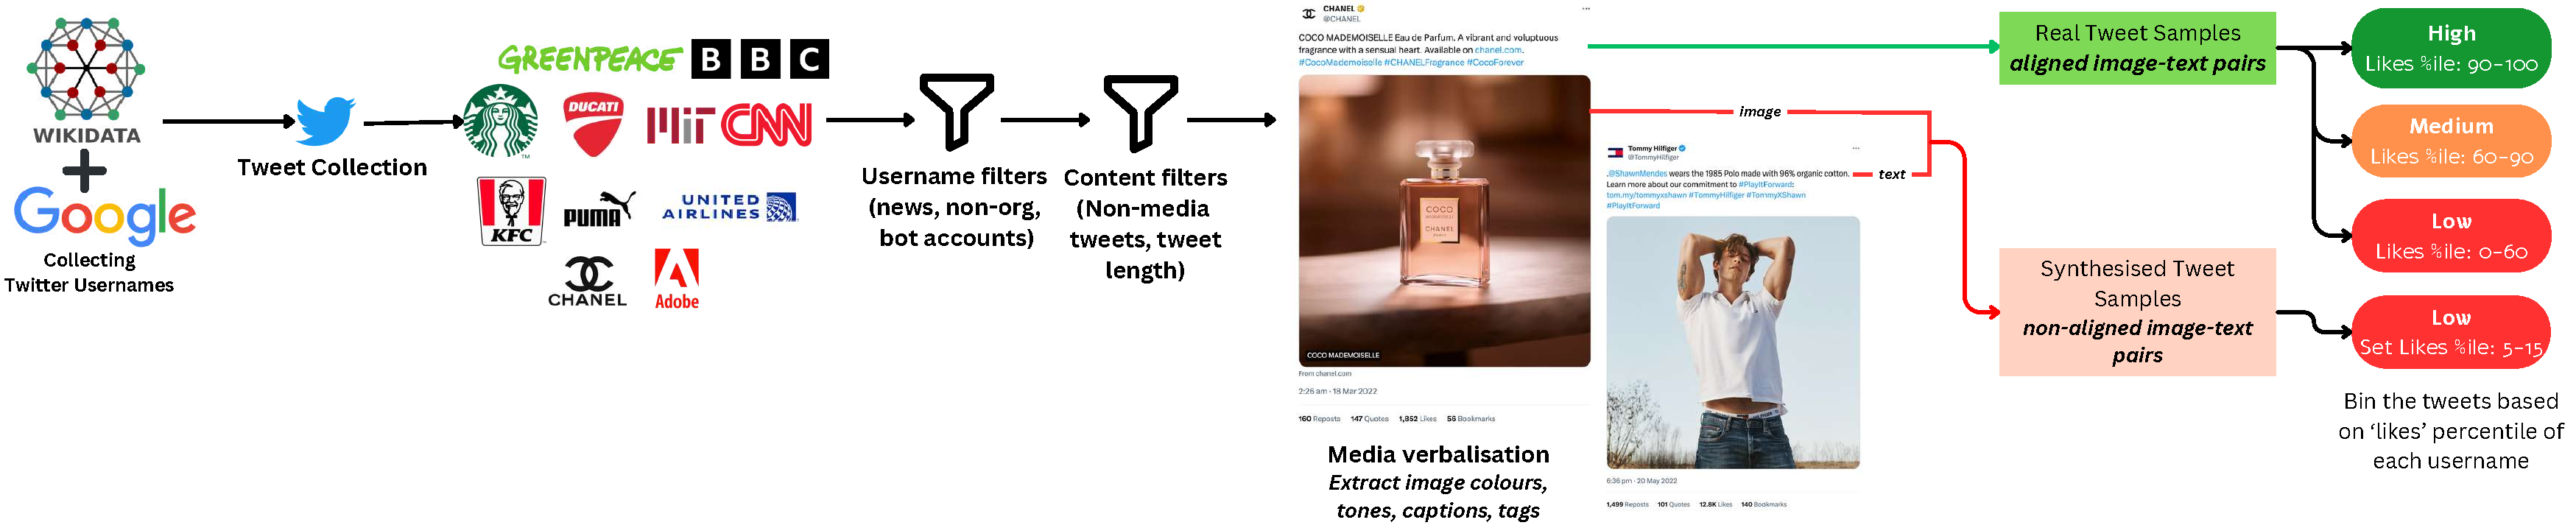
\includegraphics[width=1.5\textwidth]{images/boigbench_data_creation_compressed.pdf}
         %\vspace*{-8pt}
         \caption{\label{fig:EngagingImageNet_data_creation}
         Figure illustrating the steps involved in the creation of the EngagingImageNet dataset.}
         %\vspace*{-10pt}
       \end{figure*}
\end{landscape} 
 
 %%%%%%%%%%%%%%%%%%%%%%%%%%%%%%%%%%%%%%%%%%%%%%%%%
 \subsection{\textit{EngagingImageNet}: Dataset With In-The-Wild User Engagement}
 \label{ref:setup}
 \label{sec:EngagingImageNet}
 %In this section, we cover the details of the problem setup, talking about the pipeline for the systematic collection of images and their performance data. %Next, we provide detailed analysis and insights in both the datasets we use for training and evaluating our generative models. Finally, we elaborate on the techniques to train a behavior-conditioned image generation pipeline.
 
 To gain insights into image engagement and align text-to-image generation with user engagement, we start by collecting a large dataset of user engagement over images. Our data collection method involved leveraging Twitter, a platform extensively utilized by brands for various purposes such as ongoing product campaigns, sales, offers, discounts, brand building, and community engagement \cite{alalwan2017social}. Twitter user engagement metrics encompass user likes, retweets, comments, mentions, follows, clicks on embedded media, and links. However, the Twitter API provides access to only user likes, retweets, and comments for a given post, with access to comments necessitating a separate and costly call. Therefore, utilizing academic API licenses, we extracted the following data from Twitter: Tweet ID, company name, username, timestamp, tweet text, media files, and user likes. %We cover the details of the EngagingImageNet dataset creation below.
 
 
 We focus on enterprise handles for our data collection efforts since the content released by enterprises has the explicit goal of user engagement and is relatively much cleaner than user-generated content. We began by compiling a comprehensive list of company names using the Wikidata knowledge graph \cite{wikidata}, focusing on entities categorized as `business' or `enterprise'. We conducted Google searches to gather a list of all associated accounts for these companies. For example, for Adobe, this encompassed accounts like Adobe, Adobe Photoshop, Adobe Lightroom, Adobe Experience Cloud, and so forth. This method enabled us to amass a total of 10,135 enterprise Twitter handles. We then utilized the Twitter API to retrieve tweets posted by these enterprises spanning from 2007 to the closure of the Twitter API in January 2023. This effort resulted in the collection of 168 million tweets over a 17-year period, with 28.5 million of these tweets featuring various forms of media, including GIFs, images, and videos. Fig.~\ref{fig:EngagingImageNet-dataset-samples} shows several examples of media and tweets present in the EngagingImageNet. %Among tweets containing media, the average number of media items per tweet was 2.04. 
 %Further, Figs.~\ref{fig:aesthetic_score_distribution_stock},\ref{fig:aesthetic_score_distribution_EngagingImageNet} show the distribution of aesthetics between high and low KPI images, demonstrating that there is no significant difference in aesthetics between high and low KPI images.
 
 % Thus, we sample 365,129 tweets posted in 5 years from January 2018 to January 2023 by 592 Twitter handles.

\begin{table}[!tp]\centering
%\vspace*{-0.5pt}
\caption{A comparison of datasets containing image preferences}\label{tab:image_preference_datasets}
%\vspace*{-10pt}
\resizebox{\textwidth}{!}{\begin{tabular}{|c|c|c}\toprule
\textbf{Dataset} &\textbf{Size} \\\midrule
Pick-a-Pic \cite{kirstain2023pick} & \makecell{968,965 rankings originated \\from 66,798 prompts and 6,394 users} \\
\midrule
Human Preference Score \cite{Wu_2023_ICCV} & \makecell{Total of 98,807 images \\generated from 25,205 text prompts} \\
\midrule
ImageReward \cite{xu2024imagereward} & \makecell{Annotations for 8878 text prompts and \\corresponding model outputs sampled from \\ DiffusionDB, resulting in 136,892 compared pairs} \\
\midrule
EngagingImageNet (Ours) & \makecell{\textbf{28.5 million} tweets containing media, captions,\\colors, tones, and objects, and \\with user likes as engagement metric} \\
\bottomrule
\end{tabular}}
%\vspace*{-15pt}
\end{table}
 
 Next, for each username, we bin the tweets falling in the bottom 60 percentile (and having absolute likes $>$ 20), 60-90 percentile (and having absolute likes $>$ 30), and 90-100 percentile (and having absolute likes $>$ 40) of all tweets per account based on the number of user likes. These buckets are subsequently referred to as `low', `medium' and `high' liked buckets, respectively. %Further, for each username, we check if the number of tweets in each bucket is at least 100, else we discard the username. This step ensures that there are a sizeable number of tweets for each handle, preventing outliers and tweets of stray handles. 
 % \textcolor{red}{There can be multiple images in a tweet, so number of training samples are 869157. Including negative samples, the size increases to 957809 }
 The resulting dataset, EngagingImageNet, consists of 837,532 samples, having 144,905 high-liked images, 336,200 medium-liked images and 356,427 low-liked images. The high-liked tweets had an average of 2435 likes, while low-liked tweets had an average of 132 likes. 
 % Bucket-wise average of company-normalized likes percentile (0-100 scale): 
 % high-liked images: 95
 % medium-liked images: 76
 % low-liked images: 37
 Subsequently, all images were verbalized by extracting their captions using LLaVA \cite{liu2023visual}, colors and tones along with their coverage using \cite{Qin_2020_PR}. 
 % and object tags using RAM \cite{zhang2023recognize} which are further fed to Grounding DINO \cite{liu2023grounding} to obtain the object bounding boxes. 
Further details regarding the data processing are provided in Appendix \ref{sec:dataset_processing}.

% (Figure \ref{fig:EngagingImageNet_data_creation}) Figure~\ref{fig:company_tweets_vs_time} depict the distribution of likes and the number of posts over time, revealing the absence of significant seasonal patterns in the distribution of likes.

 
 %%%%%%%%%%%%%%%%%%%%%%%%%%%%%%%%%%%%%%%%%%%%%%%%%
 
 %\subsection{Stock Dataset}
 %\label{sec:Stock Dataset}
 
 %In addition to the EngagingImageNet dataset, we incorporated another dataset to evaluate the performance of utility-driven image generation. This dataset is sourced from a Stock business selling images. The dataset contains images, their captions and keywords, and their associated KPIs as the number of downloads, ``forward actions'', and impressions. Forward action is a type of non-purchase engagement metric recorded after a user clicks, paginates, or raises a license request after searching for an asset. Naturally, being non-purchase metrics, the number of forward actions and impressions is much more than the number of downloads. To create balanced subsets, we leveraged the relatively less skewed forward actions metric to divide the data into three approximately equal-sized buckets.
 
 
 
 %In the end, the high bucket contained 14,649 samples; the medium bucket had 12,834, and 20,142 in the low bucket. These samples include captions, keywords, release dates, image content, and the three KPIs. To create a test set, we randomly selected 1000 samples from each bucket, while the remaining samples were designated for the training set.
 
 \iffalse
     Number of forward actions per sample:
     \begin{itemize}
         \item High: 61.401
         \item Medium: 5.885
         \item Low: 1.644
     \end{itemize}
     Average number of objects and colours detected in images:
     \begin{itemize}
         \item Objects: 2.015
         \item Colours: 4.185
     \end{itemize}    
 \fi
 
 
 
 
 % \begin{figure*}[h]
 %   \centering
 %   \includegraphics[width=0.95\textwidth]{images/architecture_diagram_bs_reward.pdf}
 %   \caption{\label{fig:architecture_diagram}
 %   Architecture of the proposed pipeline for behaviour-optimised image generation using the method described in Section \ref{sec:Performance Aligning Stable Diffusion}.}
   
 % % Once trained, EngageNet possesses the capability to generate verbal descriptions of an image based on conditioning factors such as the marketer, time, caption, keywords, tweet text, and the specified Key Performance Indicator (KPI). EngageNet inherently understands how an image should align with a given KPI and prompt.
 % % EOIG-SD takes a prompt and generates an image, which then undergoes verbalization via image perception models. Its objective is to create images that, when verbalized, closely resemble the behavior-conditioned verbalization generated by EngageNet. The verbalized output of EOIG-SD is fed into the reward model. Using the logits provided by EngageNet, a reward is computed for EOIG-SD, indicating how closely this verbalized output aligns with EngageNet. This reward value serves as feedback for EOIG-SD in the form of policy gradient, aiding in its continual improvement and refinement within the image generation process. Thus, this pipeline trains EOIG-SD to generate behavior-optimized images by gradually aligning its output with EngageNet. 
 % % \vspace*{-3mm}
 % %\cy{I guess the green one is the reward model? Should label it out if so. Also, why is there a graph of the reward? How do you construct it?} \cy{Also, how do you go from the orange block to get prompts for EngageNet and the caption and keywords for EOIG-SD?}
 %   % Utilizing EngageNet's logits as a reward signal, we train EOIG-SD.
 %   % The verbalized output is then fed into the reward model, which compares it against the logits provided by EngageNet. This comparison facilitates the calculation of a reward value for EOIG-SD. This reward value is further employed as feedback for EOIG-SD in the form of policy gradient, aiding in its continual improvement and refinement within the image generation process. \cy{can you 1) make the font size in the figures larger; 2) describe the pipeline in the title?}
 % \end{figure*}
 
 



 
 
 %%%%%%%%%%%%%%%%%%%%%%%%%%%%%%%%%%%%%%%%%%%%%%%%%
 \subsection{\textit{EngageNet}: Measuring Image Engagement}
 \label{sec:Measuring Engagement: EngageNet and Engagement Arena}

In this section, we cover the alignment of existing metrics with viewer engagement and design a model to measure the progress of image generation models with the goal of engagement.
 \subsubsection{Alignment of Existing Models with Viewer Engagement}
  In order to measure the engagement potential of generated images, we first check the alignment of the most popular existing metrics used for evaluating text-to-image models with viewer engagement. For this, we calculate the Pearson correlation of Aesthetic score \cite{schuhmann2022laion}, CLIP score \cite{radford2021learning}, Pickscore \cite{kirstain2023pick}, ImageReward \cite{xu2024imagereward}, and Human Preference Score (HPS) \cite{Wu_2023_ICCV} with ground truth brand-wise normalized user likes (0-100) from EngagingImageNet. Table~\ref{tab:EngageNet_kpi_prediction_results} presents the results of this analysis. Clearly, the existing metrics are not aligned with user engagement. 
 

 This non-alignment can be attributed to the following reasons. Models like PickScore, HPS, and ImageReward are optimized for creator preferences captured on platforms like Discord or custom web applications rather than user (viewer) preferences. The feedback from image creators or communities on these platforms tends to reflect artistic or stylistic biases that do not necessarily correlate with user engagement metrics like clicks, likes, or shares. 
 Further, these models evaluate images in isolation, without considering the contextual information about the image, such as company, time of releasing the image, \textit{etc.}, reducing their effectiveness in predicting user engagement. This suggests that the existing metrics are not designed to capture the user engagement of images.
 %Similarly, the reliability of current image evaluation metrics like Fréchet Inception Distance (FID) \cite{} in reflecting human preferences remains questionable. These metrics utilize a classification-based CNN trained on ImageNet, which has been shown to prioritize image texture over general content \cite{geirhos2018imagenettrained}, and misaligned with human perception \cite{wu2023better}. 
 Recent studies have employed the CLIP model as a proxy for human judgment \cite{nichol2022glide,rombach2022high}, aiming to assess the alignment between generated images and text prompts. CLIP, trained on a diverse dataset, is thought to better capture nuanced aspects of human intention. However, similar to ImageReward and PickScore, the text prompts for CLIPScore come from image creators rather than users (viewers), which again is ineffective in conforming to viewers' expectations. The aesthetic score, built on pre-trained CLIP, is trained on several datasets capturing image aesthetics. However, as Fig.~\ref{fig:metric_non_alignment_with_engagement} shows, viewer engagement is much more nuanced than what aesthetics can capture.


Next, we try in-context learning with GPT-3.5 \cite{ouyang2022training} and GPT-4-Vision \cite{openai2023gpt4} to predict viewer engagement over images. For GPT-3.5, we supply the image verbalization along with the Twitter handle and posting time, and for GPT-4-Vision, we give the actual image, the image verbalisation, the Twitter handle and posting time. We find that neither GPT-3.5 nor GPT-4 are able to predict user engagement accurately. 

%In contrast, EngageNet is trained on real-world images posted by enterprise accounts for marketing purposes, along with corresponding user engagement data. 



% Image Engagement Prediction
 \begin{table}[!tp]\centering
%\vspace*{-15pt}     
\caption{Pearson correlation between model predicted scores and image engagement measured by account normalized likes.}\label{tab:EngageNet_kpi_prediction_results}
     \resizebox{\columnwidth}{!}{
     \begin{tabular}{|c|c|c|c}\toprule
     \textbf{Model} &\textbf{Configuration} &\textbf{Pearson Correlation} \\\midrule
     PickScore \cite{kirstain2023pick} & -& 0.0734 \\
     \midrule
     ImageReward \cite{xu2024imagereward} & -& 0.0285 \\
     \midrule
     Human Preference Score \cite{Wu_2023_ICCV} & -& 0.0747 \\
     \midrule
     Aesthetic Score \cite{schuhmann2022laion} & -& 0.0674 \\
     \midrule
     CLIP Score \cite{radford2021learning} & -& 0.0423 \\
     \midrule
     \midrule
     GPT-3.5 \cite{ouyang2022training} &\makecell{3-shot In-context learning} & 0.0464\\
     \midrule
     GPT-3.5 \cite{ouyang2022training} &\makecell{5-shot In-context learning} & 0.0351\\
     \midrule
     GPT-4V \cite{openai2023gpt4} &\makecell{3-shot In-context learning} & 0.1453\\
     \midrule
     GPT-4V \cite{openai2023gpt4} &\makecell{5-shot In-context learning} & 0.1264\\
     \midrule
     \midrule
     EngageNet &\makecell{Trained on random KPI, Tested on actual KPI} & 0.0617\\
     \midrule
     EngageNet &\makecell{Trained without MSE loss} & 0.5821 \\
     \midrule
     EngageNet &\makecell{Trained without date input} & 0.5365 \\
     \midrule
     EngageNet &\makecell{Trained without company input} & 0.5226 \\
     \midrule
     EngageNet &\makecell{Trained without date and company input} & 0.4476 \\
     \midrule
     EngageNet &\makecell{Trained without negative samples} & 0.6051 \\
     \midrule
     EngageNet &\makecell{Trained with MSE loss and negative samples} & 0.6248 \\
     \midrule
     EngageNet &Oracle & 0.8682\\
     \bottomrule
     \end{tabular}}
     %\vspace*{-10pt}
 \end{table}




 
 \subsubsection{EngageNet Model To Align With Viewer Engagement}
 \label{sec:EngageNet}
 
 Since the existing approaches do not show acceptable performance for predicting user engagement over images, we, therefore, train our own engagement-aware vision-language model (VLM) model, EngageNet. To this end, we perform visual instruction fine-tuning of LLaVA-1.5 \cite{liu2023visual} on the EngagingImageNet train dataset (Figure \ref{fig:EngageNet_training}). We design an instruction (Listing~\ref{EngageNet:behaviour_simulation-1}) for the VLM to predict the normalized likes of an image on a 0-100 scale, also conditioned on metadata comprising the marketer (company), image resolution, image colours and tones with their spatial coverage, image description and tags, and the date of releasing the image on social media. 


% Contrastive samples
 We also augment EngagingImageNet with synthetic data samples. For this, we randomly sample 25\% tweets from the high and medium likes buckets of each company and pair the tweet with an unrelated image from a different tweet. The corresponding likes is set to a low value, randomly sampled from the range 5-15. The resulting samples are called \textit{negative samples}. This helps the model with the following: (1)~it induces more sensitivity towards image features and reduces bias on tweet metadata to predict the KPI, and (2)~penalises the image if it is irrelevant to the tweet context. 
 
 Finally, we end up with a dataset of 957,809 samples, which we split into training and testing sets. We randomly sampled nearly 2000 samples from each bucket for testing, with the remaining samples used for training.  
 
 % Inputs to EngageNet BS reward model:
 % \begin{itemize}
 %     \item actual image
 %     \item company
 %     \item image resolution
 %     \item image colours and spatial coverage
 %     \item marketer's intended image caption 
 %     \item marketer's intended image tags
 %     \item date of posting the tweet
 
 % Output from EngageNet: normalised KPI (0-100)
     
 % \end{itemize}
 
 % In Listings~\ref{EngageNet:verbalization-1}-\ref{}, we provide the image caption, keywords, date, and required KPI as inputs to the model. Our aim is to train the model to predict the colors, tones, objects, and locations that should be reflected in the image. Moreover, we observe improved learning in the language model for behavior-conditioned image generation when introducing a 20\% noise in the behavior. We then task the model to rectify this noise in the output, simultaneously generating the verbalization of the behavior-conditioned image in Listings~\ref{EngageNet:verbalization-3}-\ref{EngageNet:verbalization-4}.
 %Since we didn't have an input image as part of behavior instruction tuning, we used only the language branch of Llama.  
 
 
 % Results

 
 % Mean squared error as auxiliary loss for EngageNet


 
 Since EngageNet is trained to predict the KPI of an image, we additionally model the problem as a regression task. We attach a two-layered MLP network on top of the last layer of hidden states of the decoder module to predict the scalar KPI from EngageNet. Therefore, while typically language models are trained on cross-entropy loss $L_{CE}$, we also use mean squared error $L_{MSE}$ as an auxiliary loss to train EngageNet%, similar to \cite{zhou2024customization}
 . This is because $L_{MSE}$ is more sensitive to the difference between the predicted and actual KPI values, which is crucial to better guide EngageNet to learn the image KPI prediction task. Thus, the final loss function for EngageNet is given by:
 \begin{equation}
     L_{EOIG} = L_{CE} + \lambda L_{MSE}
 \end{equation}
 where $\lambda$ is a hyperparameter that controls the weight of the auxiliary loss. We set $\lambda = 0.1$ in our experiments. We find that EngageNet demonstrates strong performance at predicting user engagement over images, achieving a Pearson correlation of ~0.62 with ground truth user likes (Table \ref{tab:EngageNet_kpi_prediction_results}).



\begin{figure}[!tb]
% \vspace*{-15pt}
\centering
     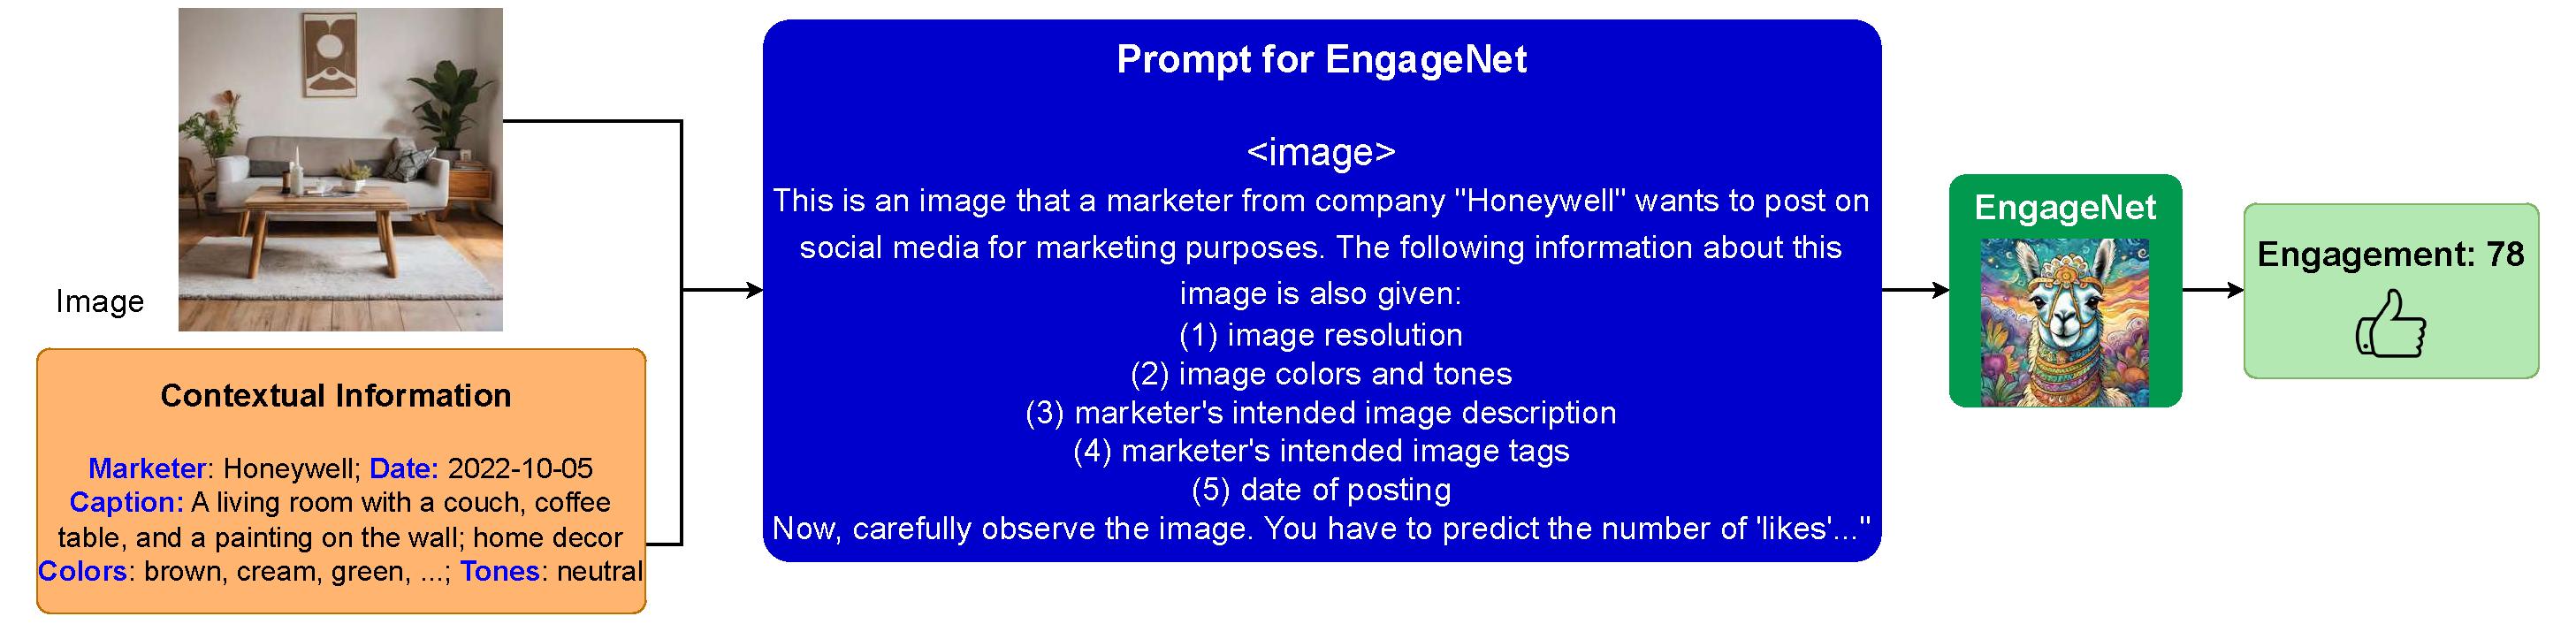
\includegraphics[width=1\columnwidth]{images/boigllm_vift_compressed.pdf}
     %\vspace*{-8pt}
     \caption{\label{fig:EngageNet_training}
     Visual Instruction Finetuning of EngageNet on EngagingImageNet dataset. The EngageNet model is trained to predict the KPI of an image on a 0-100 scale, conditioned on marketer provided metadata comprising the company, image resolution, image colours and tones with their spatial coverage, marketer's intended image description and tags, and the date of releasing the image on social media.
     }
%\vspace*{-10pt}
\end{figure}


 
%\textbf{Ablation study:} 
We perform an ablation study to understand the impact of different components of the instruction on the performance of EngageNet. If EngageNet is not supplied with contextual information such as marketer company and the time of posting the image in the input, the correlation of its predictions with ground truth account normalized likes drops significantly (0.62 to 0.44). This indicates that the company and the time of posting are important components of the instruction for EngageNet to predict user engagement accurately.  We also attempt to determine the impact of the auxiliary MSE loss adopted for training EngageNet. The MSE loss increases the correlation from 0.58 to 0.62, indicating that the auxiliary loss improves the performance of EngageNet. The MSE loss makes the model more sensitive to the difference between predicted and actual scores. 

 
We also conduct an experiment to investigate the signal present in the EngagingImageNet dataset. For this, we train EngageNet on the EngagingImageNet dataset but with randomly sampled KPI values. We then evaluate the model on the EngagingImageNet test dataset with actual KPI values. In this case, the correlation of EngageNet's predictions with ground truth user likes is nearly zero, indicating that the KPI values in the EngagingImageNet dataset are crucial for EngageNet to learn predicting user engagement accurately. 
 
 
Additionally, we evaluate the impact of adding negative samples to the training data. These samples are constructed by sampling images and other inputs in the instruction from different tweets, such that they are not aligned, and then setting the normalized likes to a very low value. Although we find that the addition of negative samples does not significantly impact the correlation of EngageNet, however it does help in improving the robustness of the model. This is because EngageNet learns to penalize images that are not aligned with the other inputs in the instruction. This is crucial for leveraging EngageNet as a reward model for engagement-optimized image generation as described in Section \ref{sec:Performance Aligning Stable Diffusion}. Since we propose to also utilize EngageNet as an oracle for ranking models in the Engagement Arena, we train EngageNet on the entire EngagingImageNet dataset, \textit{i.e.}, with both train and test data. In this configuration, EngageNet accomplishes a high correlation of 0.87 with ground truth user likes, which establishes its effectiveness to be used as an oracle. 
 


 
 
 \iffalse
     \begin{itemize}
         \item Explicitly asking model to pay attention to engagement tokens  
         \item Noisy engagement in input, exact engagement + image tokens in output
         \item Noisy engagement in input, exact engagement in output
         \item No engagement in input, exact engagement in output
     \end{itemize}
 
     We verbalise images by extracting the following key image attributes:
 \begin{itemize}
     \item colours and tones \cite{}
     \item objects and their bounding boxes: Firstly, image tags are obtained using the Recognise Anything Model (RAM) \cite{}. These tags are fed to Grounding DINO \cite{} to obtain the bounding box coordinates of the image
 \end{itemize}
 
 Model used: Visual instruction fine-tuned Llama \cite{} using Llama-2 as backbone. 
 Reason: Visual instruction fine-tuning is expected to develop better image understanding.
 \fi
 
 
 
 
 
 
 
 
 %%%%%%%%%%%%%%%%%%%%%%%%%%%%%%%%%%%%%%%%%%%%%%%%%

 \subsection{Methods to Improve Image Engagement}
 \label{sec:methods_to_improve_images}
 We explore three methods for optimizing the text-to-image generation process to generate more engaging images. These include run-time and train-time optimizations: conditioning of text-to-image models on better prompts, supervised fine-tuning of stable diffusion on high-liked images, and reinforcement learning to align stable diffusion with EngageNet-based reward scores. 
 The first method operates in the natural language domain at run-time, generating a description of how an engagement-optimized image should look like. On the other hand, the other two operate in the vision domain, generating actual engagement-optimized pixels by training the U-Net module of stable diffusion. We cover each of them next.
 
 

 
 
 %%%%%%%%%%%%%%%%%%%%%%%%%%%%%%%%%%%%%%%%%%%%%%%%%
 \subsubsection{Conditioning Stable Diffusion on More Engaging Prompts}
 \label{sec:caption_improve}

In the EngagingImageNet dataset, we observe that some images having similar themes but different details received vastly different levels of user engagement. 
For instance, consider the following pair of image captions: 
(1)~"A living room having a couch and coffee table with a rug in front." 
(2)~"A living room with large windows having a couch, coffee table and a rug"
Despite both images depicting a similar scene (Figure \ref{fig:sd_prompt_improve}), the first image received low engagement, while the second image garnered high engagement. In this case, the difference in engagement can likely be attributed to the presence of elements, such as large windows and natural light in the second image, which makes the living room appear bigger and more appealing to a viewer. Such observations motivated us to exploit patterns related to certain image aspects that can boost engagement. We further extend this analysis for images posted by a few companies in Appendix \ref{sec:Analysing Visual Aspects that Drive Engagement}.
 
 Therefore, in this method (Figure \ref{fig:sd_prompt_improve}), we attempt to alter the text prompts fed to the diffusion model such that the improved captions 
 % describe the characteristics of an image that is likely to be more performant on average. 
incorporate characteristics that have been empirically shown to boost image performance.
 For this, we adopt a retrieval framework described as follows. Using FAISS \cite{johnson2019billion, douze2024faiss}, we index the vector embeddings of captions belonging to images in the high performance data subset of the EngagingImageNet train data as described in Section \ref{sec:EngagingImageNet}. Next, for every image caption in the low performance subset of the test data, we retrieve the semantically most similar caption from the corpus of high-performing images. If the similarity level is above a certain threshold $\tau$, the retrieved captions thus obtained are passed as input to the diffusion model for generating more performant images, otherwise the original caption is used for image generation.


 
 %%%%%%%%%%%%%%%%%%%%%%%%%%%%%%%%%%%%%%%%%%%%%%%%%


 % Behavior Optimised Image Description
 \begin{table*}[!b]\centering
 %\vspace*{-10pt}
     \caption{Results reveal the significant gains achieved in improving the engagement of low-liked subset of the EngagingImageNet dataset by enhancing the image descriptions fed to a text-to-image model, as described in Section \ref{sec:caption_improve}. }\label{tab:caption_improve}
     %\vspace*{-7pt}
     \resizebox{\textwidth}{!}{
         \begin{tabular}{cccccc}\toprule
             \textbf{Images} &\textbf{Training Config} &\multicolumn{2}{c}{\textbf{Oracle Engagement Reward}} &\textbf{Engagement reward increase} \\\cmidrule{1-5}
             & &w/o prompt improvement &w/ prompt improvement & \\\midrule
             DALL.E-2 &N.A. &42.1459 &45.7077 &8.45\% \\
             SD 1.4 &N.A. &38.7680 &43.8173 &13.02\% \\
             EOIG SD 1.4 &RLHF-ES &40.2037 &46.1218 &14.72\% \\
             EOIG SD 1.4 &RLHF-DSG &39.4950 &44.8116 &13.46\% \\
             EOIG SD 1.4 &\makecell[l]{Preferred\\Finetuning (PFT)} &43.1206 &46.6490 &8.18\% \\
             SD 1.5 &N.A. &39.4001 &44.3287 &12.51\% \\
             SD 2.1 &N.A. &45.4952 &49.6946 &9.23\% \\
             Pixart-alpha &N.A. &44.7305 &49.3322 &10.29\% \\
             Pixart-sigma &N.A. &46.2870 &51.4671 &11.19\% \\
             SD XL &N.A. &49.1094 &53.8602 &9.67\% \\
             SD XL - DPO &N.A. &51.3786 &54.5863 &6.24\% \\
             SD 3 Medium &N.A. &50.6578 &55.0841 &8.74\% \\
             Flux.1-dev &N.A. &48.7226 &53.7209 &10.26\% \\
             Ground Truth &N.A. &41.2152 &56.7533 &37.70\% \\
             \midrule
             & & \multicolumn{2}{c}{\textbf{Average Increase in Engagement}} &\textbf{12.41\%} \\
             % \multicolumn{4}{c}{\textbf{Average Increase}} &10.63\% \\
             \bottomrule
             \end{tabular}}
             %\vspace*{-10pt}
 \end{table*}
 
 
 %%%%%%%%%%%%%%%%%%%%%%%%%%%%%%%%%%%%%%%%%%%%%%%%%

 
 
 \subsubsection{Preferred Finetuning on High-Engagement Images}
 \label{sec:Finetuning Stable Diffusion on High-KPI Images}
 
 Several prior studies have demonstrated the feasibility of learning styles through stable diffusion by fine-tuning the model \cite{pinkney2022text-to-pokemon,cjwbw2022waifudiffusion,prompthero2023openjourneyv2,everaert2023diffusion}. These approaches typically involve fine-tuning the U-Net architecture within the Stable Diffusion framework using a set of images exhibiting the desired style.
 For instance, \citet{everaert2023diffusion} proposed a method to finetune Stable Diffusion to adapt it to target styles like \textit{anime sketches}, \textit{American comics}, \textit{Pokemon}, \textit{starry night}, \textit{etc.}
 
 In this work, we attempt to explore whether the diffusion model can learn patterns associated with higher user engagement, analogous to learning visual styles. To this end, we performed fine-tuning of the base Stable Diffusion U-Net on the preferred data distribution, containing high liked images sampled from the EngagingImageNet train set (Figure \ref{fig:sd_preferred_finetuning}). We call this process, \textbf{Preferred Finetuning}. The model was finetuned for $50$ epochs, following the procedure outlined by \citet{vonplaten2023stablediffusion}. The model minimizes the standard denoising score matching loss \cite{ho2020denoising, ho2022classifier}, which measures how well the model predicts the noise added to the image during the diffusion process:
\begin{equation}
    L_{\text{denoise}} = \mathbb{E}_{\mathbf{x}_0, \boldsymbol{\epsilon}, t} \left[ \|\boldsymbol{\epsilon} - \boldsymbol{\epsilon}_{\theta}(\mathbf{x}_t, t, \mathbf{c})\|^2 \right]
\end{equation}


where $\mathbf{x}_0$ is the original image, $\mathbf{x}_t$ is the noisy image at time step $t$, generated by adding noise $\boldsymbol{\epsilon}$, $\boldsymbol{\epsilon}_{\theta}(\mathbf{x}_t, t, \mathbf{c})$ is the predicted noise from the model given the noisy image $\mathbf{x}_t$, time step $t$ and conditioning information $\mathbf{c}$ \textit{i.e.}, text prompt fed as input to the diffusion model. 




 % However, our observations reveal that fine-tuning the stable diffusion model does not yield improvements in rewards calculated over the validation set across subsequent epochs.
 %\cy{refer to some results here}.
 % \textcolor{red}{expand and include SD loss function}
 
 
 
 
 %%%%%%%%%%%%%%%%%%%%%%%%%%%%%%%%%%%%%%%%%%%%%%%%%
 
 
   
 
 
 \subsubsection{Aligning Stable Diffusion With Engagement}
 \label{sec:Performance Aligning Stable Diffusion}
 %\cy{Maybe use this title?: Reward Modeling to Aligh Stable Diffusion} 

 \citet{black2023training} proposed denoising diffusion policy optimization (DDPO), a policy gradient algorithm which frames the denoising process as a multi-step decision-making problem. The authors showed that DDPO can be employed to finetune text-to-image diffusion models to align their outputs with a variety of reward functions including image compressibility, aesthetic quality and image-prompt alignment, among others. Therefore, we explore the use of reinforcement learning to optimize diffusion models to improve the engagement potential of their generated images. To this end, we leverage EngageNet as a reward model to align a pre-trained stable diffusion model using DDPO algorithm to produce more engaging images. The entire process of alignment is shown in Figures~\ref{fig:architecture_diagram_ddpo_cs_reward}, \ref{fig:architecture_diagram_ddpo_bs_reward} in the appendix. 
 % The policy gradient feedback loop shown in the figure for aligning the stable diffusion model is done using DDPO algorithm.
  % The denoising process in diffusion models is a multi-step recursive process with a pre-specified finite number of steps. 
  In DDPO, the denoising process is viewed as a finite horizon Markov decision process, where the state comprises of the current context, number of steps left in the process and the current denoised image. The action to be taken is to predict the next image using this state. 
 
  %\cy{I don't understand the following, can you draw a figure to help understanding as well?}:
  \noindent We experiment with two types of reward functions for finetuning stable diffusion:\\
(1) Engagement Simulation (ES): We leverage EngageNet to estimate the user engagement of images generated by stable diffusion. The reward signal is used to guide stable diffusion to generate higher engagement images as illustrated in Figure \ref{fig:architecture_diagram_ddpo_bs_reward}. The resulting diffusion model is called EOIG-SD (RLHF-ES).\\
% EngageNet predicts the image KPI on a scale of 0-100, conditioned on the image prompt, marketer information, and the date of posting the image. We use this predicted KPI as the reward signal for the stable diffusion model. The reward signal is used to update the stable diffusion model's parameters using the DDPO \cite{black2023training} algorithm.
(2) Design Specification Generation (DSG): We train an alternate version of EngageNet to produce the design specification of an image, based on conditioning factors such as the company, time, image caption and viewer likes. This model learns to predict verbalized image descriptions comprising colors and tones with their spatial coverage, as well as objects with their locations, that should be reflected in an image, for a given engagement level and caption. The detailed method and results of EngageNet trained on this task are explained in Appendix \ref{sec:EngageNet Content Simulation}. 
Next, we utilise this EngageNet as a reward model to train stable diffusion such that the images generated by it have a design specification aligned with those of higher engagement images as shown in Figure \ref{fig:architecture_diagram_ddpo_cs_reward}.
EOIG-SD (RLHF-DSG) takes a text prompt and generates an image, which then undergoes verbalization via image perception models. 
Its objective is to create images that, when verbalized, closely resemble the engagement-conditioned verbalization generated by EngageNet. Thus, we ask EngageNet to provide the logits for this image verbalization, using which a reward is computed for EOIG-SD, indicating how closely this verbalized output aligns with EngageNet. This reward value serves as feedback for EOIG-SD in the form of policy gradient, aiding in its continual improvement and refinement within the image generation process. Only high engagement samples are used in the training process.
The details of this method are described in Appendix \ref{sec: Performance Aligning Stable Diffusion - Content Simulation}.

     
 






 
 
 
 % Behavior Optimised Image Generation
 \begin{table*}[!b]\centering
 %\vspace*{-10pt}
     \caption{Comparing the performance gains on the EngagingImageNet test dataset, resulting from train-time engagement-optimization methods applied on stable diffusion, as described in Sections \ref{sec:Finetuning Stable Diffusion on High-KPI Images} and \ref{sec:Performance Aligning Stable Diffusion}.}\label{tab:Eoig_twitter_results}
     %\vspace*{-5pt}
     \resizebox{\textwidth}{!}{
         \begin{tabular}{lccccccccc}\toprule
             \textbf{Images} &\textbf{Training Config} &\textbf{Bucket} &\textbf{\makecell{Engagement\\Reward}} &\textbf{\makecell{Engagement\\Increase}} &\textbf{Aesthetic Score} &\textbf{CLIP Score} &\textbf{FID} &\textbf{PickScore} \\\midrule
             \multirow{3}{*}{Ground Truth} &\multirow{3}{*}{N.A.} &High &90.9526 &N.A. &5.1006 & 32.6343 &N.A. &20.9470 \\
             & &Medium &74.3535 &N.A. &5.0940 & 32.4867 &N.A. &20.9351 \\
             & &Low &41.2152 &N.A. &5.0518 & 32.2012 &N.A. &20.7406 \\\midrule\midrule
             \multirow{3}{*}{SD 1.4} &\multirow{3}{*}{N.A.} &High &56.1489 &N.A. &5.2029 &33.0830 &24.6631 &17.3514 \\
             & &Medium &51.6949 &N.A. &5.1634 &32.9173 &23.4434 &17.3344 \\
             & &Low &38.7680 &N.A. &5.1662 &32.8339 &24.2607 &17.3262 \\\midrule
             \multirow{3}{*}{EOIG SD 1.4} &\multirow{3}{*}{\makecell{Preferred Finetuning \\(PFT) on \\High engagement Images}} &High &62.0390 &10.49\% &4.8090 &32.4524 &24.9370 &17.3070 \\
             & &Medium &56.1082 &8.54\% &4.8387 &32.3923 &23.0904 &17.3239 \\
             & &Low &43.1206 &11.23\% &4.8108 &32.2960 &23.5885 &17.2932 \\\midrule
             \multirow{3}{*}{EOIG SD 1.4} &\multirow{3}{*}{RLHF - ES} &High &58.2724 &3.78\% &5.1828 &33.2891 &23.8656 &17.4113 \\
             & &Medium &53.1004 &2.72\% &5.1686 &33.2845 &22.7157 &17.3802 \\
             & &Low &40.2037 &3.70\% &5.1629 &32.9468 &24.1780 &17.3672 \\\midrule
             \multirow{3}{*}{EOIG SD 1.4} &\multirow{3}{*}{RLHF - DSG} &High &57.9188 &3.15\% &5.2495 &33.1072 &23.9144 &17.3577 \\
             & &Medium &52.9765 &2.48\% &5.2187 &33.0991 &23.3626 &17.3486 \\
             & &Low &39.4950 &1.88\% &5.2336 &32.9716 &24.2147 &17.3277 \\
             \bottomrule
             \end{tabular}}
  %\vspace*{-15pt}
\end{table*}
 


 %%%%%%%%%%%%%%%%%%%%%%%%%%
% EOIG Generated Samples

\begin{figure}[!t]
  \centering
  %\vspace*{-15pt}
  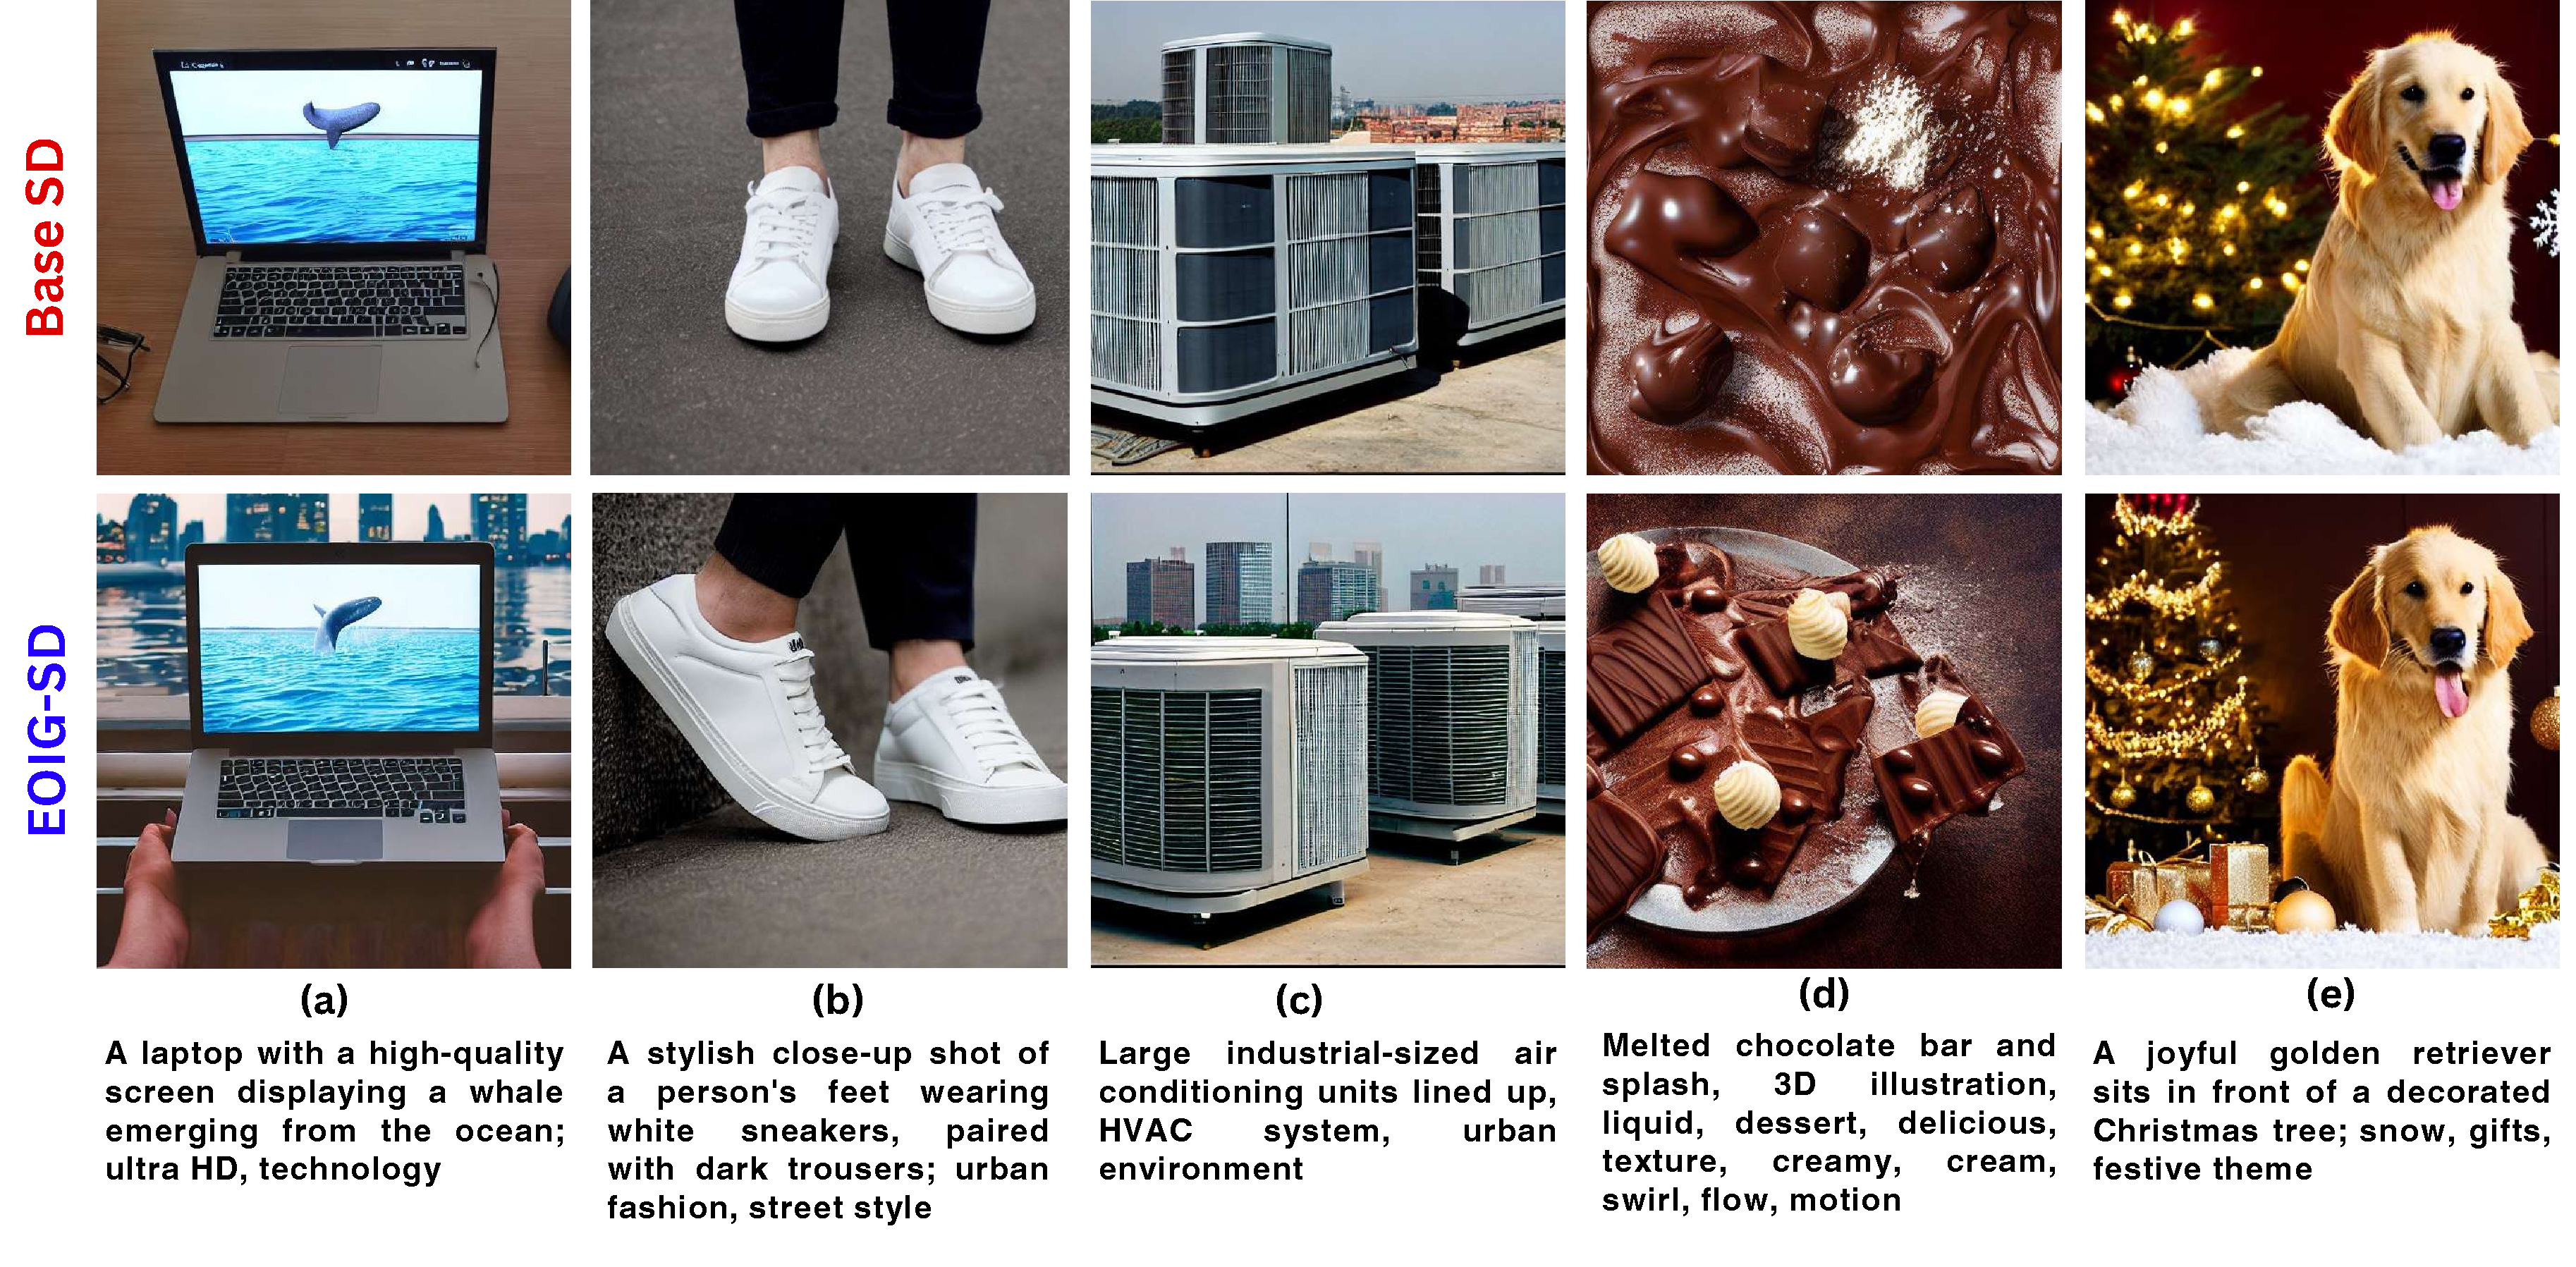
\includegraphics[width=0.95\textwidth]{images/marketing-images-comparison_compressed.pdf}
  %\vspace*{-10pt}
  \caption{\small{Comparison of generated images - EOIG-SD \textit{vs} Base stable diffusion. Engagement optimization helps the model to learn to generate persuasion skills. EOIG-SD generates better product photography (a,c,d), model photography (b), generates images with social appeal and social identity (a,c), and learns temporal patterns (e) (prominently Christmas-themed image of dog)}
  \label{img:comparison-marketing-image}
  }
  %\vspace*{-15pt}
\end{figure}

%%%%%%%%%%%%%%%%%%%%%%%%%
 
 
 
 \subsubsection{Evaluating the Methods Adopted for Engagement-Optimization}
 \textbf{Run-time optimization:}
 Firstly, we investigate the impact of using better prompts to condition the text-to-image generation process as described in Section \ref{sec:caption_improve}. The results are summarised in Table \ref{tab:caption_improve}. By retrieving semantically similar captions from the corpus of high-liked images, visual characteristics that have been empirically shown to enhance image engagement get incorporated in the text prompt.
 Therefore, after applying this method, we observe a significant improvement in the engagement of low-liked subset of the EngagingImageNet test dataset, consistent across multiple text-to-image models, both open-source and closed-source. This method is highly effective as it is able to produce images with higher engagement without any additional training of the diffusion model. 
We observe that, on average, an improvement in the prompt results in an improvement of 12.4\% in engagement. The improvement is observed in models across all sizes and also for models trained on high-engagement images (EOIG-SD). % To understand what aspects in an image can lead to higher engagement, we conducted an analysis... % in progress
 % \textcolor{red}{Explain more: give a before-after example of the prompts and mention a particular aspect in the improved prompts that may appeal more to users.}
 

 
 \textbf{Train-time optimization:}
 Next, we present the results of the methods (\S\ref{sec:Finetuning Stable Diffusion on High-KPI Images}, \S\ref{sec:Performance Aligning Stable Diffusion}) adopted for engagement-optimized image generation by training the U-Net module of stable diffusion in Table~\ref{tab:Eoig_twitter_results}. We denote all the models trained using train-time optimizations like Preferred fine-tuning with EOIG (engagement optimized image generation). We compare the performance of the base stable diffusion model (SD 1.4), stable diffusion finetuned on high-engagement images (EOIG-SD PFT), and stable diffusion aligned with EngageNet-based reward functions (EOIG-SD RLHF-ES, EOIG-SD RLHF-DSG). For this, we use EngageNet-Oracle as a judge to predict the user engagement of the images generated by these models. This helps us probe the effect of different training strategies on improving the engagement capabilities of stable diffusion. Consistent with prior literature, we also include other metrics like FID \cite{heusel2017gans}, aesthetics \cite{schuhmann2022laion}, CLIP score \cite{radford2021learning}, and PickScore \cite{kirstain2023pick}. 


% Results (Table~\ref{tab:Eoig_twitter_results}) reveal that this approach of fine-tuning of the U-Net module on the preferred data distribution yields noticeable improvement in the engagement of the generated images. We observe that engagement increases across all the three buckets of engagement. 

 
 % Results summary
 % Eoig SD - PFT: finetuning on preferred data distribution, i.e. high KPI images significantly improves the results across all KPI buckets
 % Eoig SD - RLHF BS also improves the results, but the improvement is not as significant as Eoig SD - PFT
 % Eoig SD - RLHF CS also improves the results, but the improvement is not as significant as Eoig SD - PFT
 
 The results indicate that while all the training methods improve the engagement capabilities of stable diffusion, however, the extent of improvement varies widely. We find that finetuning the stable diffusion model on preferred data distribution, i.e. high-engagement samples from the EngagingImageNet dataset yields significant gains in the engagement potential of the generated images. This is evident from the consistent increase in the predicted user engagement of the generated images across all engagement buckets. % However, we find that the mean aesthetic score slightly drops in this case.
 Next, we discover that using EngageNet-based reward functions to align the stable diffusion model also results in better performance. %and aesthetics. 
 However, the improvement in image engagement is not as significant as that achieved by the previous methods. 
 Other metrics like CLIP score, PickScore and FID do not vary significantly across the EngagingImageNet buckets and largely remain unaffected after training stable diffusion in both the above regimes. This further corroborates their non-alignment with image engagement. 

 
 
 
 
 % Next, we compare three models for the task of behavior-optimized image generation: base stable diffusion, stable diffusion finetuned on high-KPI samples, and performance-aligned stable diffusion (EOIG-SD). Consistent with prior RLHF literature \cite{black2023training,kirstain2023pick,xu2023imagereward,fan2023dpok,wu2023better}, we evaluate these models on rewards provided by EngageNet. We also include other metrics like FID \cite{heusel2017gans}, aesthetics \cite{schuhmann2022laion}, and CLIP score \cite{radford2021learning}. The results are summarized in Table~\ref{tab:twitter_data_scores}. We see that EOIG-SD outperforms base stable diffusion and high-KPI finetuned stable diffusion. Intriguingly, further finetuning the stable diffusion on high-KPI samples results in a decreased mean reward. Figs.~\ref{fig:journey of EOIG-SD images},\ref{img:comparison-marketing-image} visually depict the progression of several images during EOIG-SD training.
 
 
 % Next, we evaluate the side effects of EngageNet's reward on EOIG-SD training. 
 % We notice (Table~\ref{tab:twitter_data_scores}) that as a result of EngageNet reward, in spite of not being directly targeted, aesthetics gets optimized across all KPI buckets for both datasets. This could be a side effect of optimizing on marketing images, which are often of higher aesthetics than images sourced from other image datasets. 
 Next, we discuss the side effects of training stable diffusion using the above methods.
 As a consequence of training on engaging images, we find that stable diffusion learns to generate images with certain persuasion strategies \cite{singla2022persuasion}. For instance, Fig.~\ref{img:comparison-marketing-image} shows several examples of product and model photography generated by EOIG-SD and base SD, demonstrating EOIG-SD's biases towards certain persuasion strategies such as social appeal and social identity, commonly observed in marketing scenarios \cite{singla2022persuasion} but ignored in general photography.


\textbf{Combination of Train-time and Run-time optimizations:} In our experiments, we gauge the impact of different methods in improving image engagement by comparing the results of both train-time (\S\ref{sec:Finetuning Stable Diffusion on High-KPI Images}, \S\ref{sec:Performance Aligning Stable Diffusion}) and run-time (\S\ref{sec:caption_improve}) optimisations, as well as their combination.
% Describe results:
% Eoig PFT w/ better prompts
% Eoig RLHF-BS w/ better prompts
% Eoig RLHF-CS w/ better prompts
Stable Diffusion 1.4 \cite{rombach2022high}, serves as the baseline model. In Table \ref{tab:caption_improve}, we observe that when each method is applied individually, such as using better prompts at run-time or training the diffusion model through supervised finetuning or using reinforcement learning, it results in measurable improvements in image engagement over the baseline.
However, the most significant improvements are seen when supervised finetuning or reinforcement learning is combined with better prompts at run-time.
This demonstrates that coupling train-time and run-time optimisations has a synergistic effect, resulting in higher engagement levels than each method applied alone.


 
 
 %%%%%%%%%%%%%%%%%%%%%%%%%%%%%%%%%%%%%%%%%%%%%%%%%
 \subsection{\textit{Engagement Arena}: Measuring Engagement Capabilities of Text-to-Image Models}
 \label{sec:image_persuasion_arena}

% Introduce what are you planning to do in this section
% List all the models - 1 paragraphs
% Comparing general models and the models with three improvements - 2-5 paragraphs
% Last paragraph - Other metrics are not substantially impacted
 
 
 Motivated by the work of LMSYS and similar benchmarks \cite{chiang2024chatbotarenaopenplatform}, we propose \textit{Engagement Arena} as a platform to evaluate the capability of text-to-image models to generate engaging images. We run a tournament on a common set of prompts from the EngagingImageNet test set. We leverage EngageNet as an oracle for \textit{Engagement Arena} to compute the Elo ratings of various open-source text-to-image models, such as Stable Diffusion 3 Medium \cite{esser2024scaling}, Flux.1-dev \cite{blackforestlabs2024}, Stable Diffusion XL \cite{podell2023sdxl}, Stable Diffusion XL-DPO \cite{wallace2024diffusion}, Pixart-sigma \cite{chen2024pixart}, Pixart-alpha \cite{chen2024pixartalpha}, Stable Diffusion 2.1, Stable Diffusion 1.5, Stable Diffusion 1.4, \cite{rombach2022high}, \textit{etc.}, and closed-source models like DALL.E-2 \cite{ramesh2022hierarchical}. Figure ~\ref{img:image_engagement_arena} shows the rankings of these models. It also features the Elo ratings of ground truth images to serve as topline for benchmarking the models.
 
 In addition to helping to rank the engagement potential of generated images accurately, using EngageNet as an oracle also avoids having static benchmarks with a definitive ground truth. We encourage the research community to adopt \textit{Engagement Arena} as a basis for measuring further advances in the engagement capabilities of text-to-image modeling and incorporating user engagement into the learning process. 
 
 The arena features actual images from the EngagingImageNet dataset as a topline benchmark for the images generated by different text-to-image models. We find that Stable Diffusion 3 Medium \cite{esser2024scaling} emerges as the best performing model in the \textit{Engagement Arena}, with a win rate of 46\% over actual images (Figure \ref{img:image_persuasion_arena_win_rates}). It is followed by SDXL-DPO \cite{wallace2024diffusion} and Flux.1-dev \cite{blackforestlabs2024}. We notice a general trend that image engagement rises with the size of the text-to-image models. However, there are some exceptions to this trend. For instance, Pixart family of models (600M parameters) and EOIG-SD PFT model (860M parameters) surpass relatively larger DALL.E-2 (6.5B parameters).
 % Model size source: \cite{chen2024pixartalpha}

  
 We observe that while our EOIG-SD models trained using different methods (PFT, RLHF) outperform the equal-sized base SD 1.4 model, however there is a considerable gap between the performance of EOIG-SD and significantly larger text-to-image models leading the arena. This can be attributed to the inherent limitations of SD 1.4 in generating high-quality images, which cannot be fully overcome by the training methods explored in this work. 

% \cy{Need to show some generated image examples in the main text}
 
 %%%%%%%%%%%%%%%%%%%%%%%%%%%%%%%%%%%%%%%%%%%%%%%%%

 % Image Persuasion Arena
 \begin{figure*}[!t]
 %\vspace*{-10pt}
     \centering
     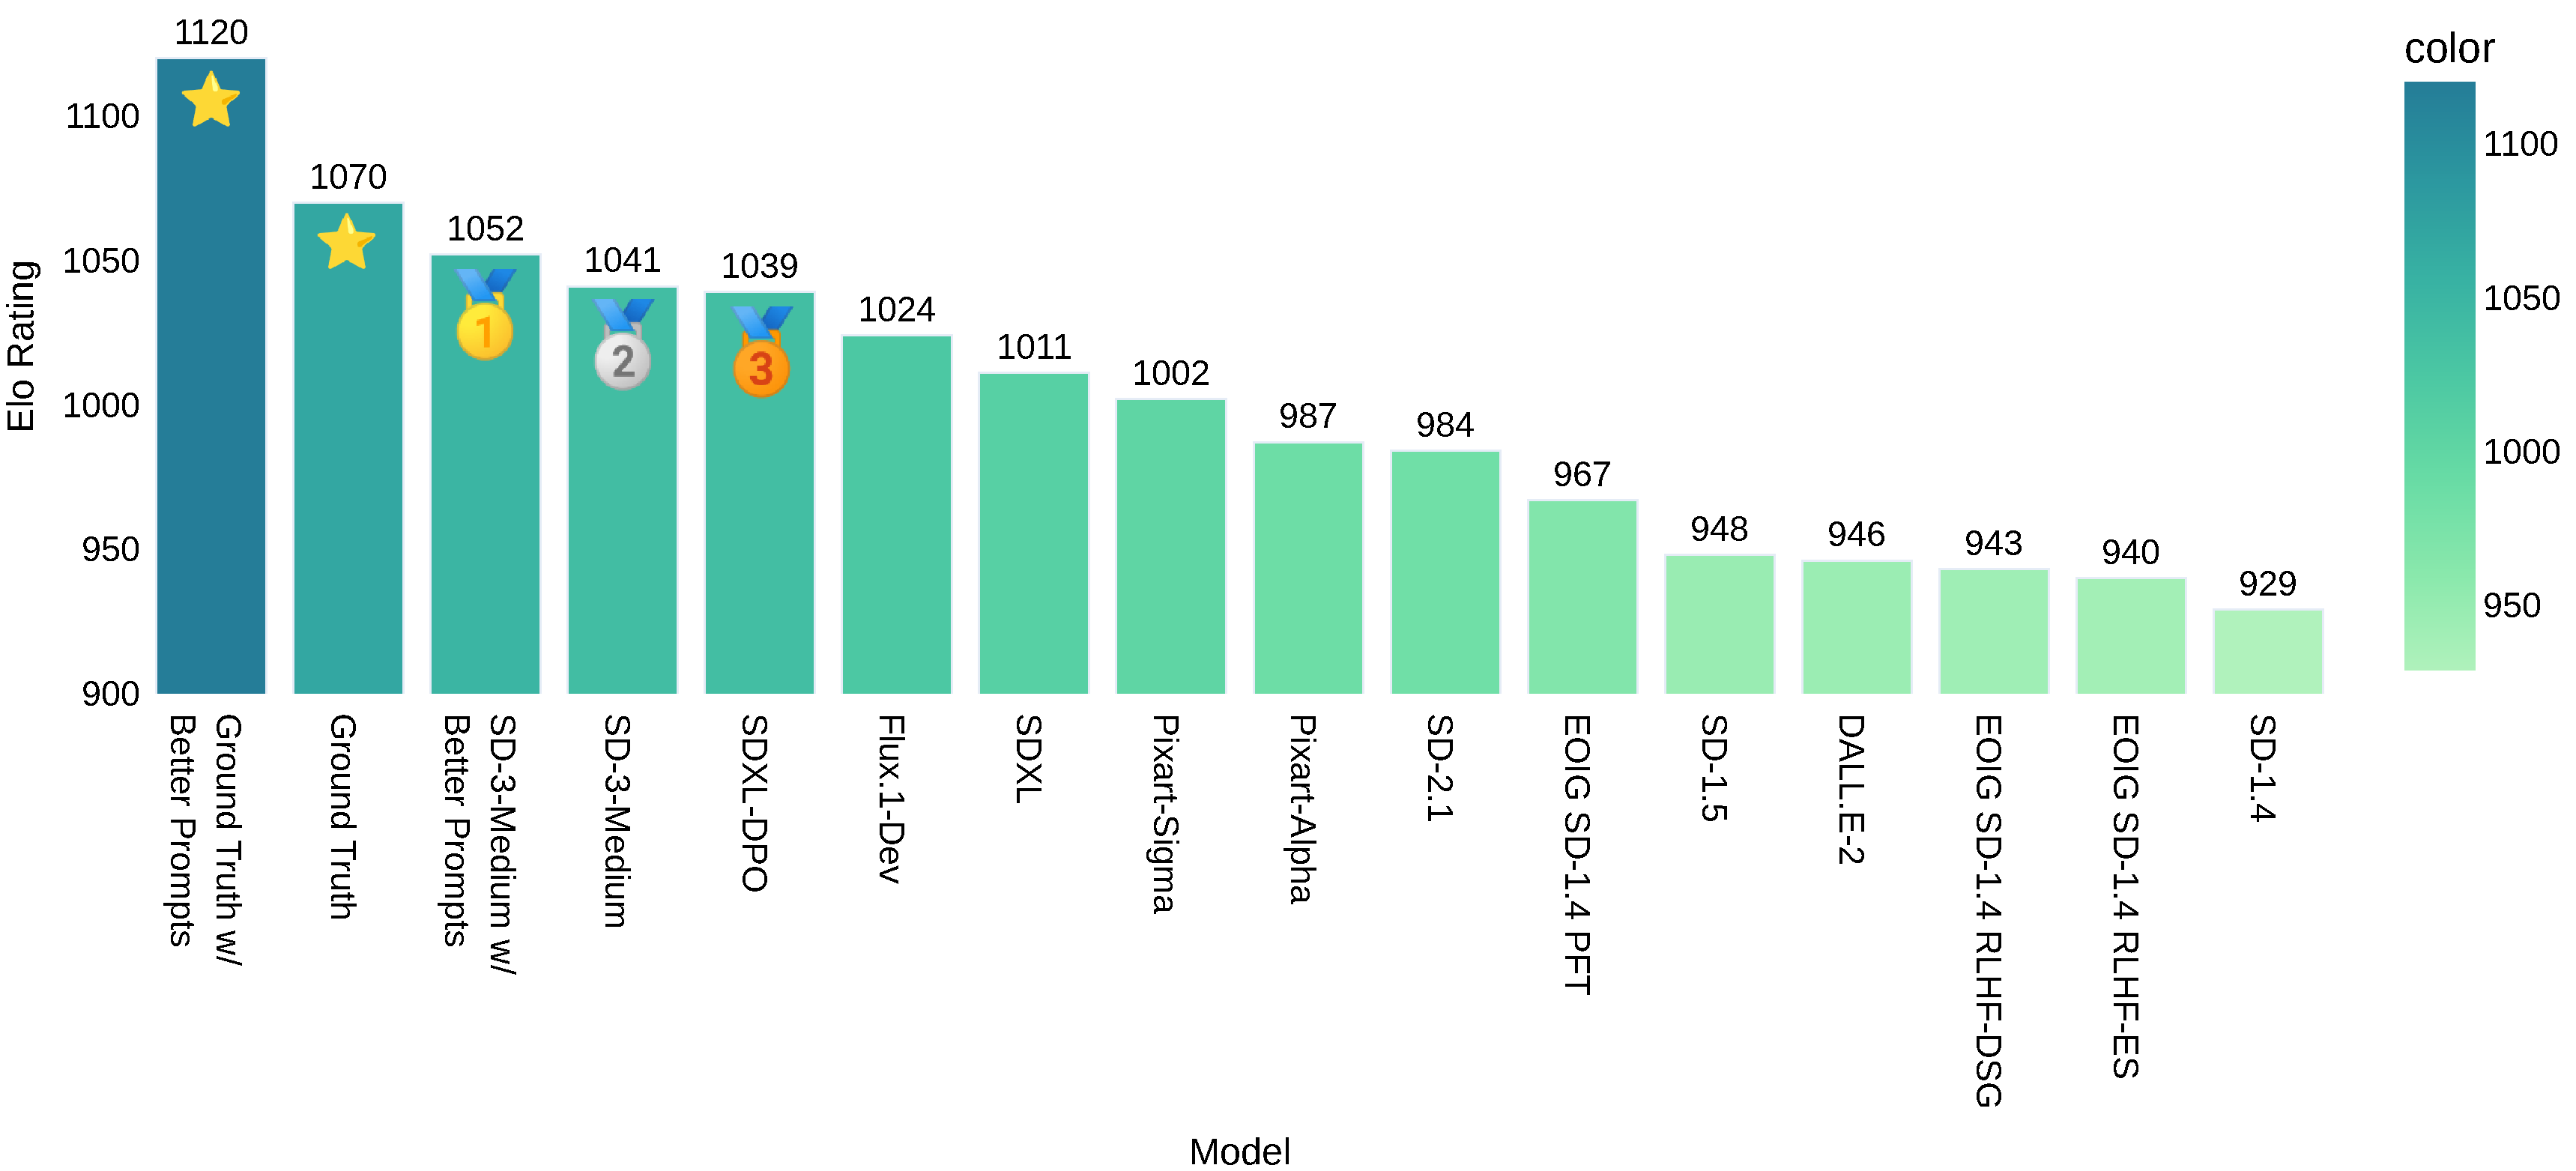
\includegraphics[width=1\textwidth]{images/image_engagement_arena.pdf}
     %\vspace*{-12pt}
     \caption{Rankings and Elo ratings of various text-to-image models in the proposed Image Engagement Arena. \label{img:image_engagement_arena}}
 %\vspace*{-15pt}
   \end{figure*}
 

 %%%%%%%%%%%%%%%%%%%%%%%%%%%%%%%%%%%%%%%%%%%%%%%%%

\subsection{Conclusion}
Image generation technologies have undergone a significant evolution, transitioning from research concepts to viable commercial products. The initial phase of image generation primarily focused on producing higher-quality images that adhere to provided prompts. In the next phase, generated images should not only meet quality standards but also align with the creator's objectives. This necessitates conditioning the image generation process based on the utility of the generated image. In marketing contexts, this utility translates into achieving higher customer engagement metrics such as likes, shares, clicks, and more. In this paper, we introduce the problem statement of engagement-optimized image generation and propose the first large-scale dataset for this purpose. Additionally, we present the results of several techniques to solve this problem both in the natural language domain by generating engagement-optimized text-prompts and in the computer vision space by generating actual engagement-optimized pixels. 
% Moreover, we demonstrate that current models, due to their lack of conditioning on engagement tokens, struggle to produce engagement-optimized images.





\subsection{Appendix}



% \begin{figure*}
%    \centering
%    \includegraphics[width=1.0\textwidth]{images/fig-1_compressed.pdf}
%    \caption{Progression of EOIG-SD generated images over the course of training: Top-1 images selected by EngageNet-based reward out of 64 generations. EngageNet optimizes for image utility (user engagement) over the course of training. While aesthetics and other metrics like prompt adherence may change over generations, the key change that EngageNet brings is the optimization of the end-objective, \textit{i.e.}, an improvement in the downstream image KPI. The end objective, in our case, is the probability of achieving a higher probability on the objective of KPI (=High). Here, we see that EngageNet also improves aesthetics and prompt adherence for a few prompts. See Fig.~\ref{img:comparison-marketing-image} for more marketing samples generated by EOIG-SD based on prompts from enterprise tweets (sourced from EngagingImageNet). \label{fig:journey of EOIG-SD images}}
%  \end{figure*}
 
 





\subsubsection{Related Work}
\label{sec:related work-eoig}
A large body of work has been done with respect to generating images from textual descriptions. These text controlled image generation models have evolved greatly from the time of GANs~\cite{goodfellow2020generative} to yield high-quality image generators based on diffusion models such as DALL-E~\cite{ramesh2021zero}, Stable Diffusion~\cite{rombach2022high} and ones that have extended these models,  that are able to follow human text instructions to a large extent. However, the metrics that these generators optimize are  Inception Score (IS)~\cite{salimans2016improved} and Fr\'echet Inception Distance (FID)~\cite{heusel2017gans}. It has been observed by multiple works for example~\cite{kirstain2023pick,Wu_2023_ICCV,xu2024imagereward} etc. that these metrics do not necessarily correspond to human preferences.

To align models with human preferences, reinforcement learning with human feedback (RLHF) has been successfully used in the LLM literature~\cite{ouyang2022training,openai2023gpt4,touvron2023llama} with algorithms such as PPO~\cite{schulman2017proximal}, DPO~\cite{rafailov2024direct} and several variants of these preference based reinforcement learning algorithms. Similar approaches have also been used in text-to-image generation models~\cite{black2023training,wallace2024diffusion}. In these approaches, the latent image generation part of the diffusion model (either UNet or a Transformer) is trained using a reward model in the case of DDPO or using user preferences directly in the case of DPO. Both these approaches involve collecting human preference datasets.

Several human preference datasets for text-to-image generation have been collected in literature. These include Pick-a-Pic dataset~\cite{kirstain2023pick}, dataset generated from the Stable Foundation Discord channel~\cite{Wu_2023_ICCV}, ImageReward dataset~\cite{xu2024imagereward} etc. The human preferences in these datasets have been collected by explicitly asking humans to state their choices.  These datasets are often accompanies with their own metrics for human preference alignment such as PickScore~\cite{kirstain2023pick}, Human Preference Score~\cite{Wu_2023_ICCV}, ImageReward score~\cite{xu2024imagereward} etc. The authors of these papers have shown that these metrics are better aligned with human preferences when compared with text-alignment scores such as CLIP score and BLIP score. However, these need not align with viewer engagement of images and hence, in our work, we use implicit data about human preferences derived from engagement metrics such as clicks, likes etc.









\subsubsection{Study with marketers}
Unlike other NLP and CV tasks where humans are the topline for any model's performance, simulating engagement is a relatively hard task for humans. It has been shown in several studies that expert human opinions fare similar to non-experts (\textit{e.g.}, \cite{tetlock2017expert,forecasting2023insights}), and the opinion of the non-expert population is just above a random coin toss for behavior simulation tasks (\textit{e.g.}, \cite{tan2014effect,isola2013makes}). Therefore, simulating engagement necessitates an automatic and reliable method to measure engagement.
 % Further, we conduct a human study where we ask expert and non-expert humans to rate images on their potential to bring in customer engagement. Our human study also replicates similar results; we find that expert and non-expert humans have an accuracy of \%, barely above random accuracy. 
  
 \begin{table}[!htp]\centering
     \resizebox{0.75\columnwidth}{!}{
         \begin{tabular}{lll}
             \toprule
             \textbf{Brand} & \textbf{Correlation Coefficient (r)} & \textbf{p-value} \\
             \midrule
             Impressions & 0.039 & 0 \\
             Clicks & 0.076 & 2.74e-61 \\
             CPC & 0.047 & 2.736e-24 \\
             CPM & 0.191 & 0.0\\
             CPP & 0.207 & 0.0\\
             \bottomrule
         \end{tabular}}
         \caption{Pearson correlation coefficients (r) and associated p-values for the relationship between marketer-allocated advertisement budget and five key performance indicators (KPIs): Impressions, Clicks, Cost Per Click (CPC), Cost Per Thousand Impressions (CPM), and Cost Per Purchase (CPP). Budget allocation serves as a proxy for marketer confidence in advertisement efficacy. Data were collected from a Fortune 500 company's marketing campaigns (n > 1,000 advertisements) over a 12-month period. Results suggest no statistically significant correlation between marketing spend and advertisement performance across all measured KPIs, indicating potential limitations in expert marketers' ability to predict advertisement success.
         \label{tab:corr-coefficients-marketer}}
 \end{table}
 
 
 We conducted several studies with both expert marketers and non-experts to estimate their capability to simulate engagement. We worked with a Fortune-500 company expert marketers for this task. Marketers usually have to run multiple advertisements for a single campaign at the same time. We estimated the correlation of their past spend data with several behavioral metrics: impressions, cost per click (CPC), cost per pixel (CPP), cost per 1000 impressions (CPM), and clicks. Table \ref{tab:corr-coefficients-marketer} shows the results of these studies where we observed that despite being experts in marketing, the budget allocation by these marketers had almost no correlation with any of the key performance indicators. 
 
 Human Eval Protocol: Particpants submitted their ideas and they were independently shown the AI generated captions fot these ideas. They are then allowed to submit their feedback in the form of like or dislike (not compulsorily). Based on their feedback they are further prompted for Reason and Feedback. We filtered the feedbacks that were related to the experimental setup. 
 % The actual protocol of the experiment can be seen in the figure \ref{fig:marketer_study_protocol} below.
 



\subsubsection{Analysing Visual Aspects that Drive Engagement}
\label{sec:Analysing Visual Aspects that Drive Engagement}
To understand the visual aspects that often lead to higher image engagement, we analysed pairs of images having same theme but different details, posted within a 45 days interval by the same account. Then pairs with vastly different engagement levels between the images were sampled. We then extracted the differences between the image pairs for a few companies using using GPT-4-Vision \cite{openai2023gpt4}. Following are some main observations. For fashion brands like Bulgari, we observe that images featuring prominent branding and dynamic backgrounds with bright colors and gradients significantly enhance engagement, as visible in Figure \ref{fig:metric_non_alignment_with_engagement} (Image pair-3).
For Gucci, engagement is driven by images that maintain a clear focus on the product, emphasizing intricate detailing and textures. Additionally, images that incorporate luxurious backgrounds contribute to higher engagement levels.
In the case of Airbnb, images that blend natural light with greenery are particularly effective in enhancing user engagement. Showcasing relatable homestay experiences aligns closely with Airbnb's branding, further driving engagement.
Meanwhile, Lenovo benefits from highlighting unique technical features and specifications while utilizing vibrant colors and high-contrast backgrounds.




\subsubsection{EngagingImageNet Filtering Steps}
\label{sec:dataset_processing}
 We sample the tweets posted in the 5 year time period from January 2018 to January 2023.
 We focus our analysis on usernames that market products or services, and thus weed out usernames belonging to categories like news and sports. Next, we check if the number of tweets posted by a username exceeds 1000, then we retain the username, else we discard remove it. This helps in removal of stray handles and ensures data quality. Further, if the number of tweets posted by a username exceeds 2000, we randomly sample 2000 tweets for this username to avoid oversampling tweets from the same username and thus compromising data variance. This step ensures that the dataset is fairly representative of different enterprise accounts. Moreover, we weed out all tweets containing media other than images and where tweet text is less than 50 characters. Also, the hyperlinks present in the tweets are masked with a $<$hyperlink$>$ placeholder. This results in 365,129 tweets posted in 5 years by 592 Twitter handles.

Since it is hard to assign KPI credit to the multiple media present in a single tweet, we assign an equal KPI credit to all the media in a tweet.




\subsubsection{EngagingImageNet Additional Details}
\label{sec:EngagingImageNet Additional Details}





%%%%%%%%%%%%%%%%%%%%%%%%%%%%%%%%%%%%%%

\begin{table}[!htp]\centering
\caption{Distribution of ground truth EngagingImageNet images }\label{tab:twitter_data_scores-ground-truth}
\scriptsize
\resizebox{0.7\textwidth}{!}{
\begin{tabular}{cccc}\toprule
\textbf{KPI}&\textbf{\# Objects} &\textbf{Aesthetic Score} &\textbf{CLIP Score} \\\midrule
High& 3.405 & 4.994 & 30.509\\
Low & 3.291 & 4.881 & 30.638\\
\bottomrule
\end{tabular}}
\end{table}


% \begin{table}[!htp]\centering
% \caption{Distribution of ground truth Stock images }\label{tab:stock_data_scores-ground-truth}
% \scriptsize
% \resizebox{0.4\textwidth}{!}{
% \begin{tabular}{cccc}\toprule
% \textbf{KPI} &\textbf{\# Objects} & \textbf{Aesthetic Score} &\textbf{CLIP Score} \\\midrule
% High & 1.993 &5.339 &30.885\\
% Medium & 2.043 & 5.351 &30.385\\
% Low & 2.011 & 5.323 &30.523\\
% \bottomrule
% \end{tabular}}
% \end{table}

% % distribution of aesthetic score for high, medium and low KPI images - Stock dataset
% \begin{figure}[t]
%     \centering
%     \begin{subfigure}[b]{0.22\textwidth}
%          \centering
%          \includegraphics[width=1\textwidth,scale=0.9]{images/stock_plots/stock_aesthetic_score_high.png}
%          \caption{}
%      \end{subfigure}
%      \begin{subfigure}[b]{0.22\textwidth}
%          \centering
%          \includegraphics[width=1\textwidth,scale=0.9]{images/stock_plots/stock_aesthetic_score_medium.png}
%          \caption{}
%      \end{subfigure}
%      \begin{subfigure}[b]{0.22\textwidth}
%          \centering
%          \includegraphics[width=1\textwidth,scale=0.9]{images/stock_plots/stock_aesthetic_score_low.png}
%          \caption{}
%      \end{subfigure}

%     \caption{Aesthetic Score distribution across High, Medium and Low KPI images in Stock dataset
%     \label{fig:aesthetic_score_distribution_stock}}
% \end{figure}


% distribution of aesthetic score for high and low KPI images
\begin{figure}[!ht]
    \centering
    \begin{subfigure}[b]{0.75\textwidth}
         \centering
         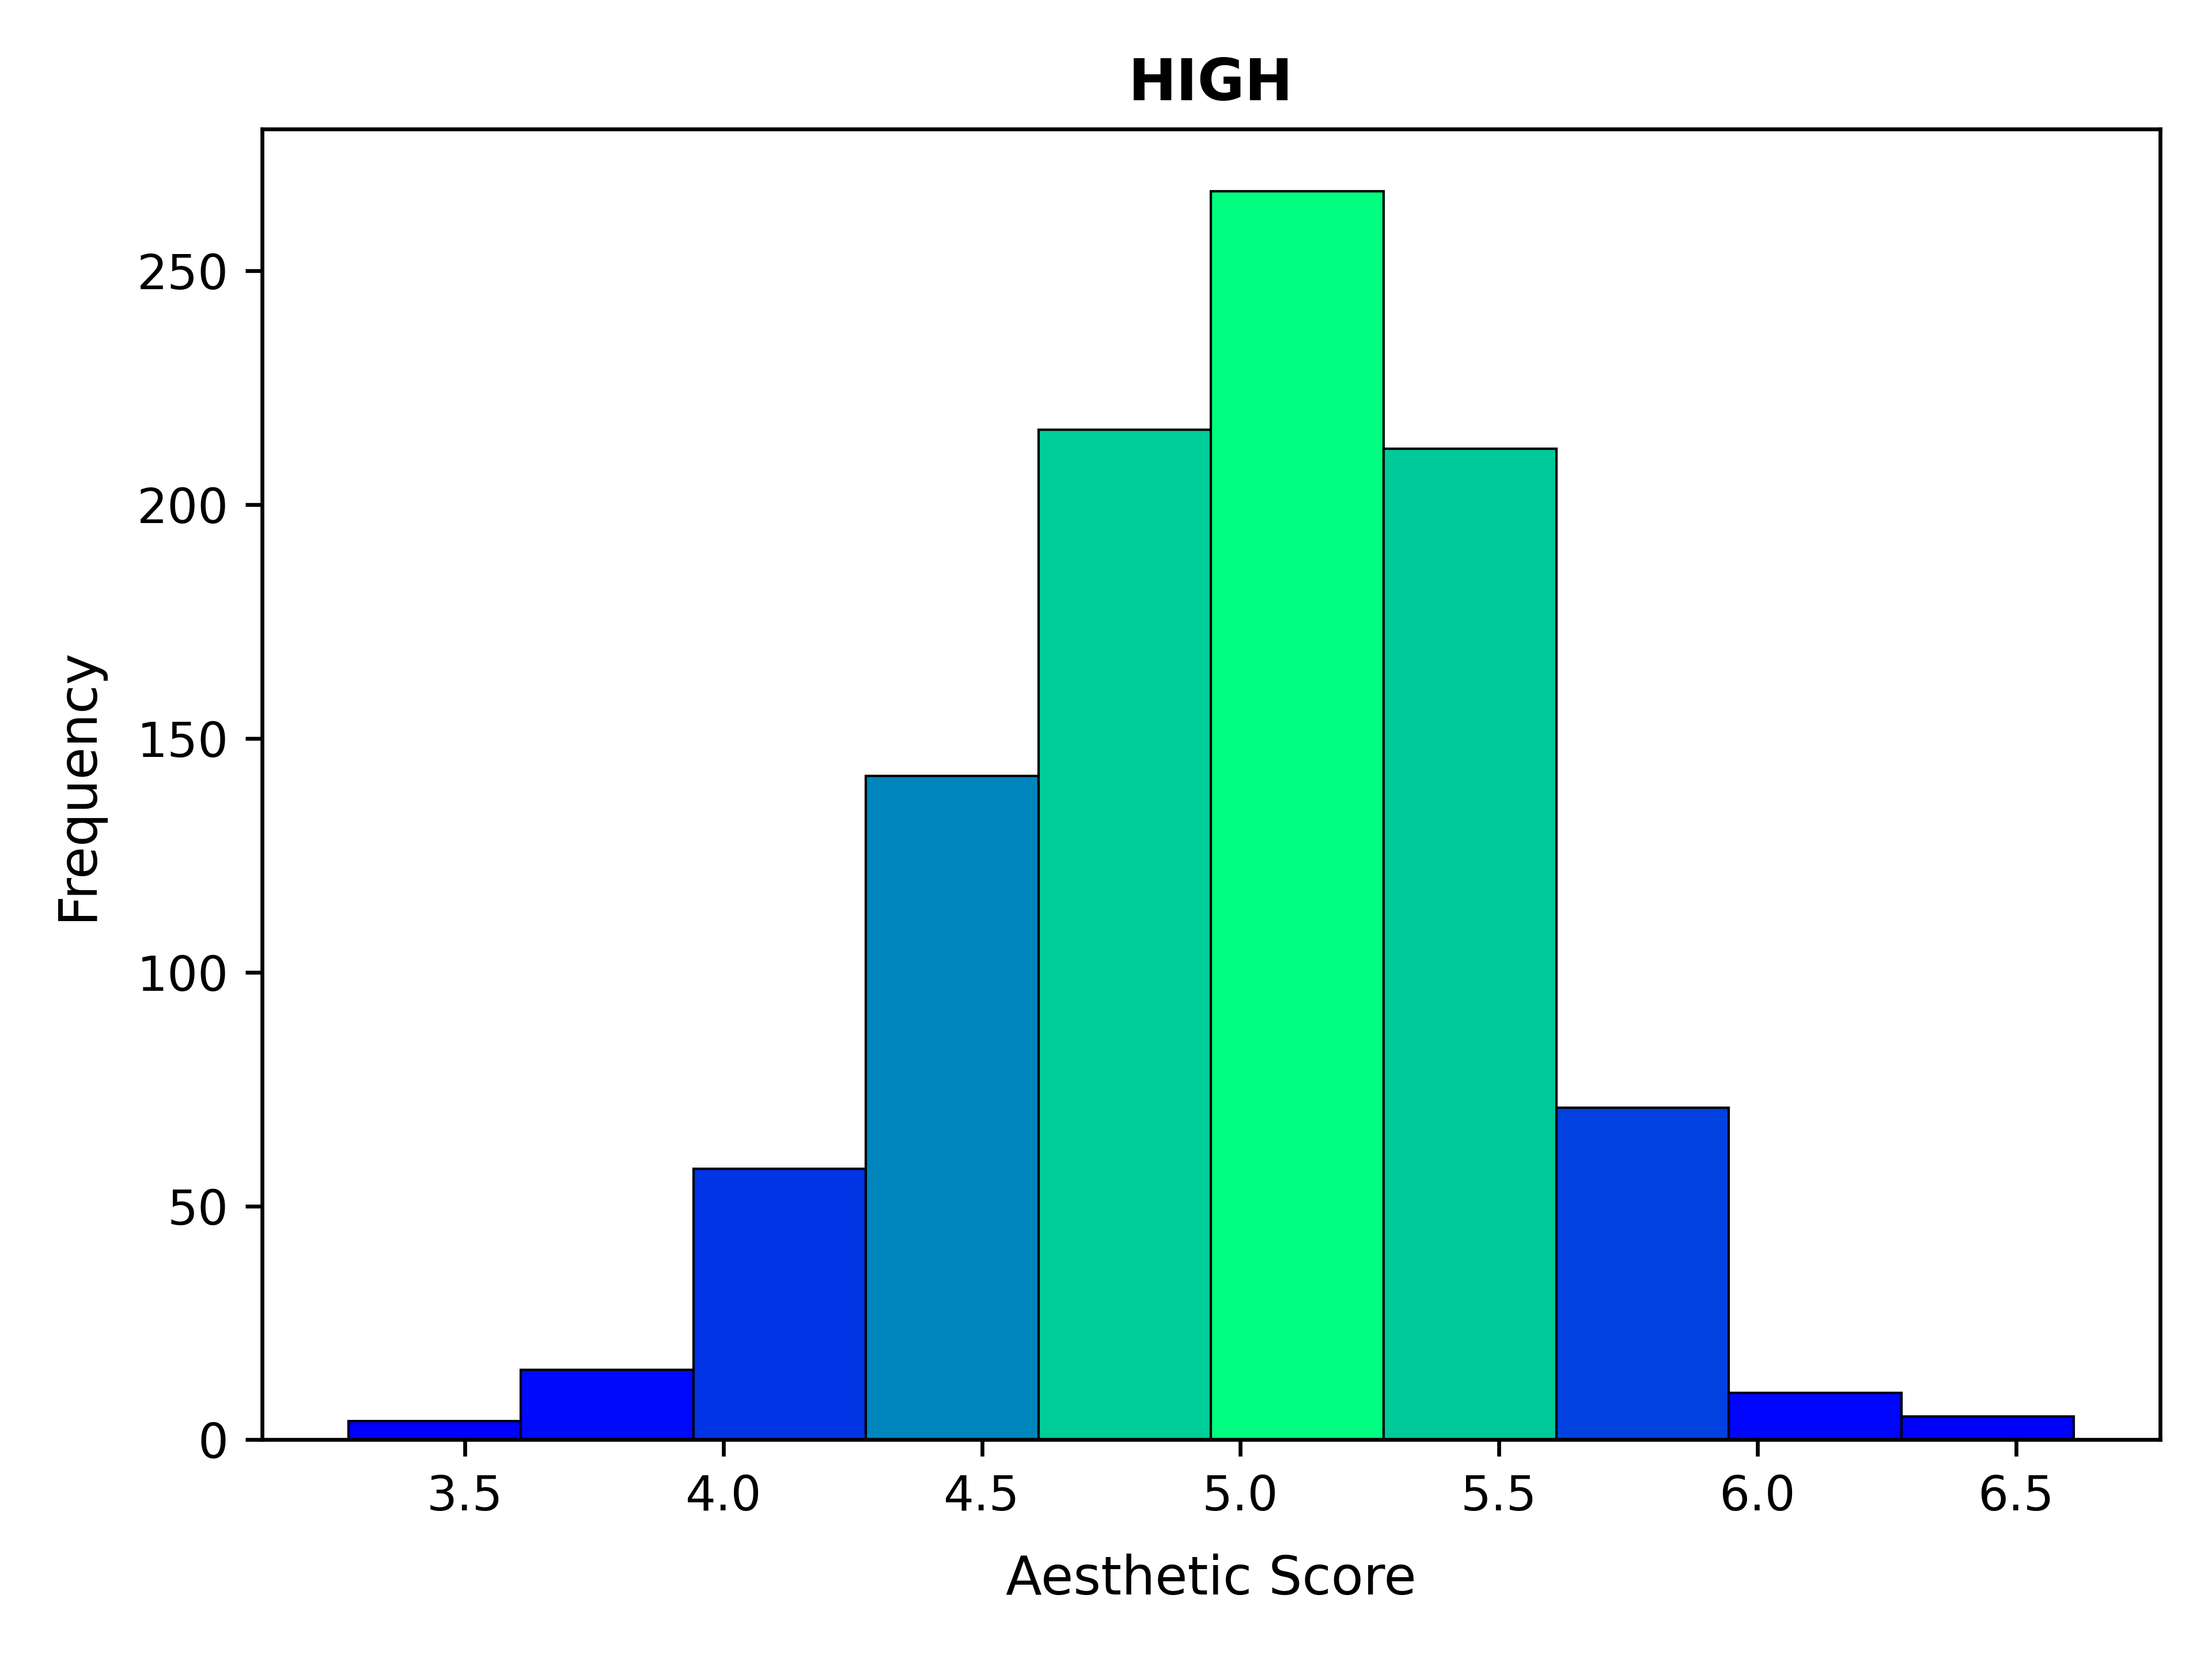
\includegraphics[width=1\textwidth,scale=0.9]{images/twitter_plots/twitter_aesthetic_score_high.png}
         \caption{}
     \end{subfigure}
     \begin{subfigure}[b]{0.75\textwidth}
         \centering
         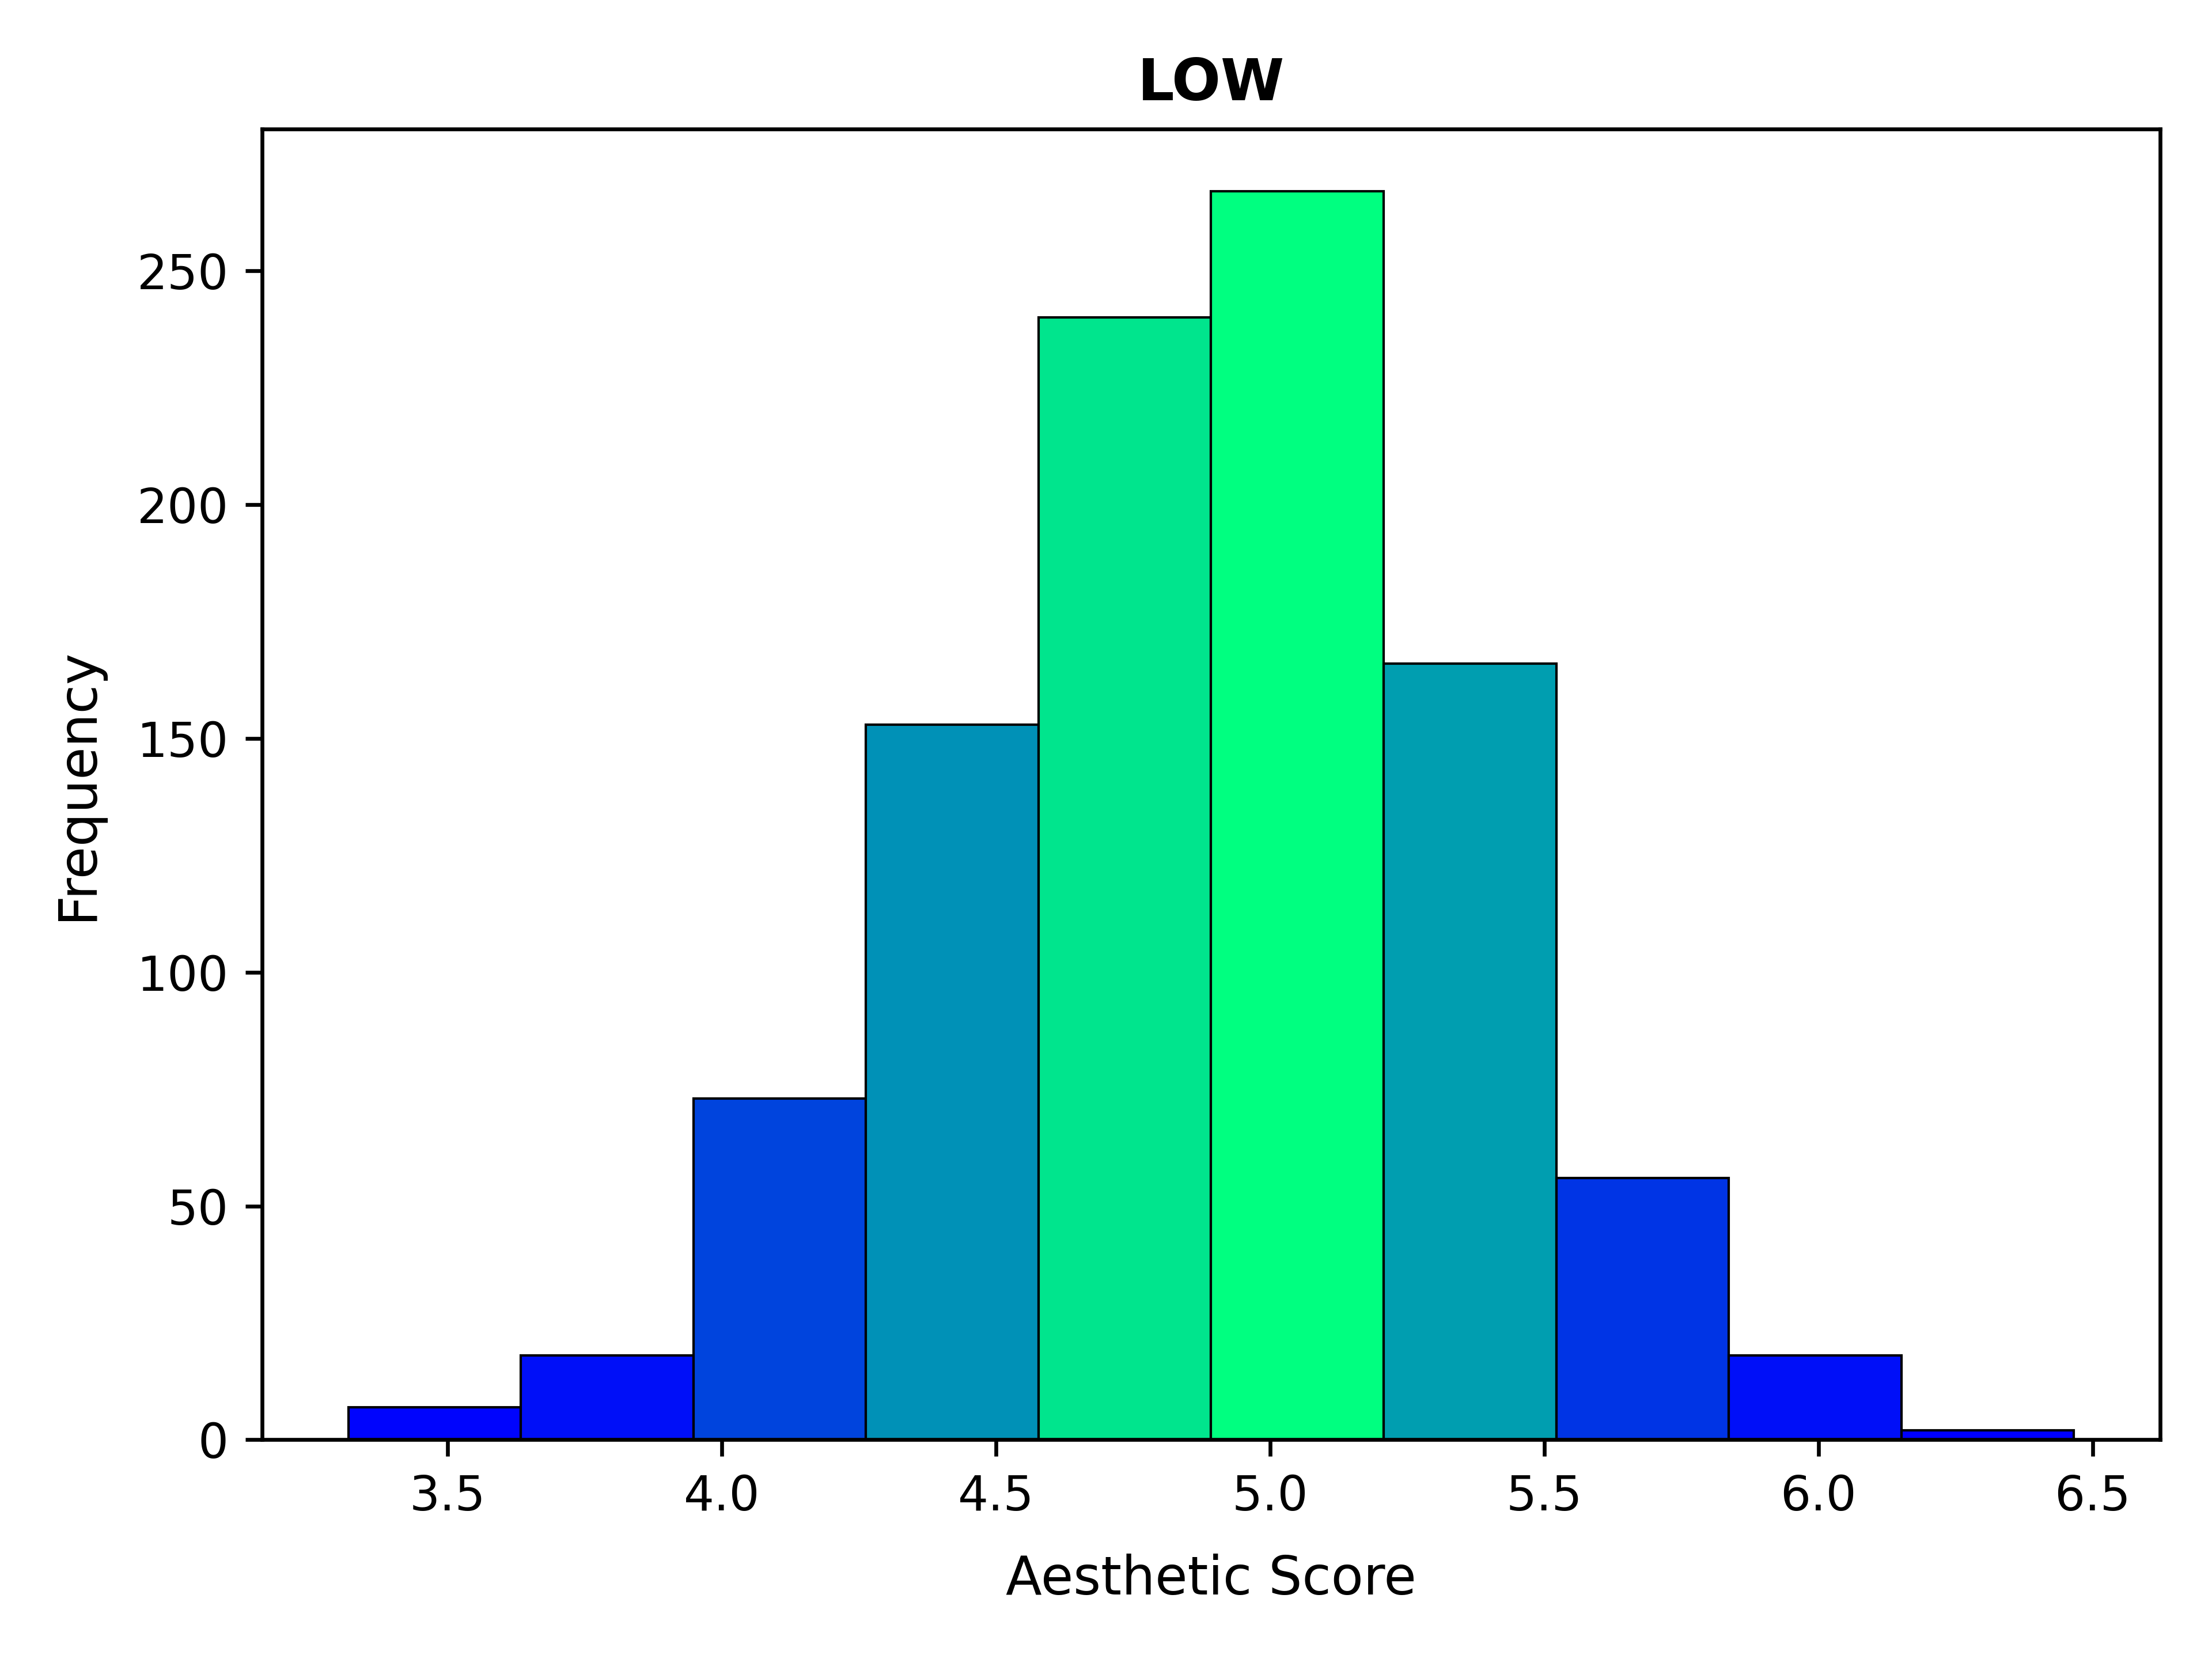
\includegraphics[width=1\textwidth,scale=0.9]{images/twitter_plots/twitter_aesthetic_score_low.png}
         \caption{}
     \end{subfigure}

    \caption{Aesthetic Score distribution across High and Low KPI images in EngagingImageNet dataset}
    \label{fig:aesthetic_score_distribution_EngagingImageNet}
\end{figure}




\begin{figure*}[t]
    \centering
    % company 1
    \begin{subfigure}[b]{0.45\textwidth}
         \centering
         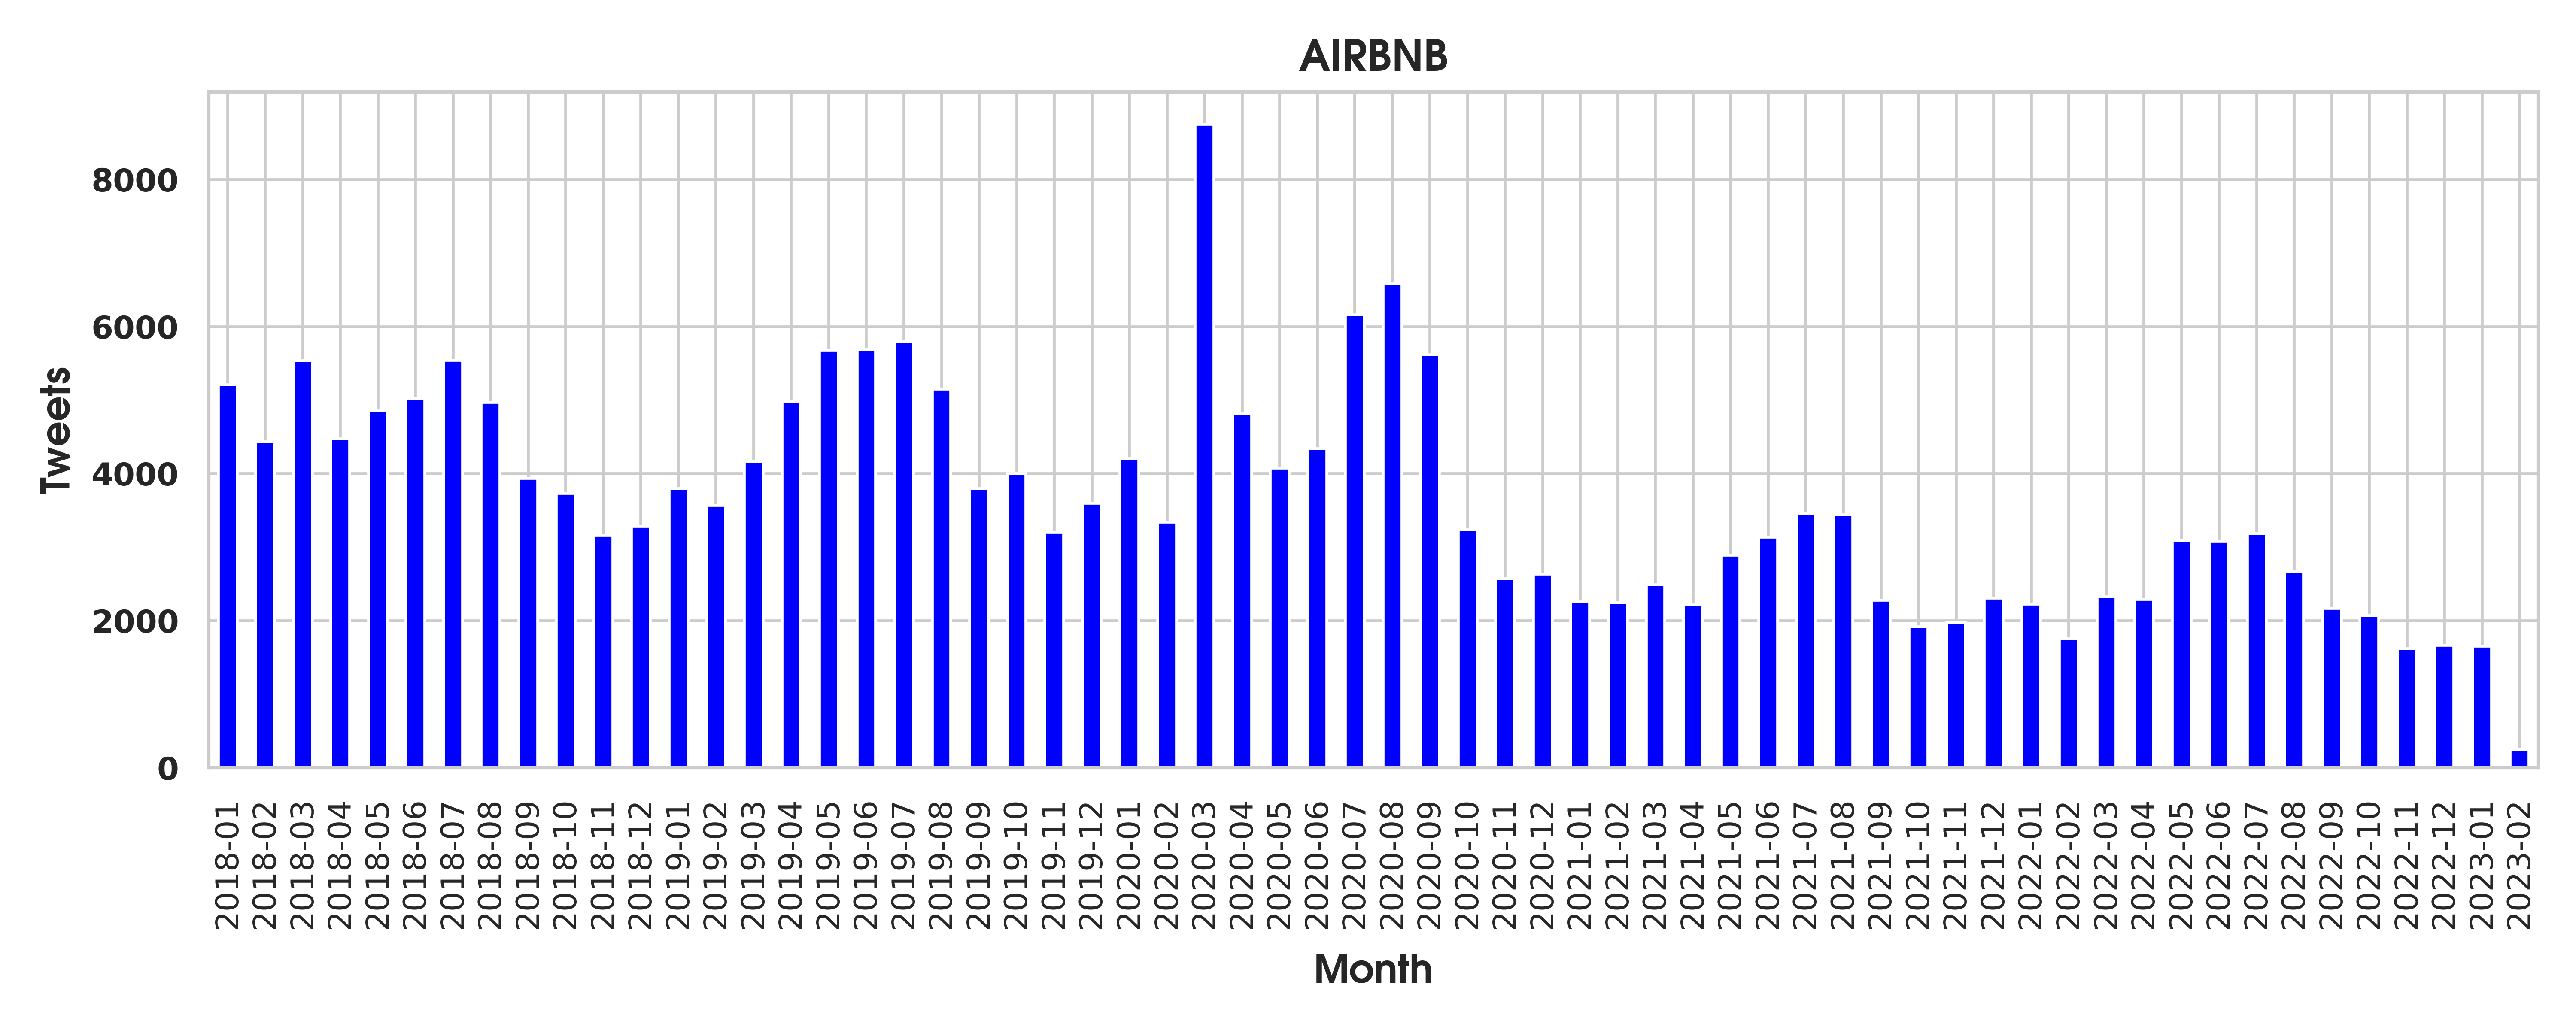
\includegraphics[width=1\textwidth,scale=1]{images/company_tweets_vs_time/airbnb_tweets.png}
         \caption{}
    \end{subfigure}
    \begin{subfigure}[b]{0.45\textwidth}
         \centering
         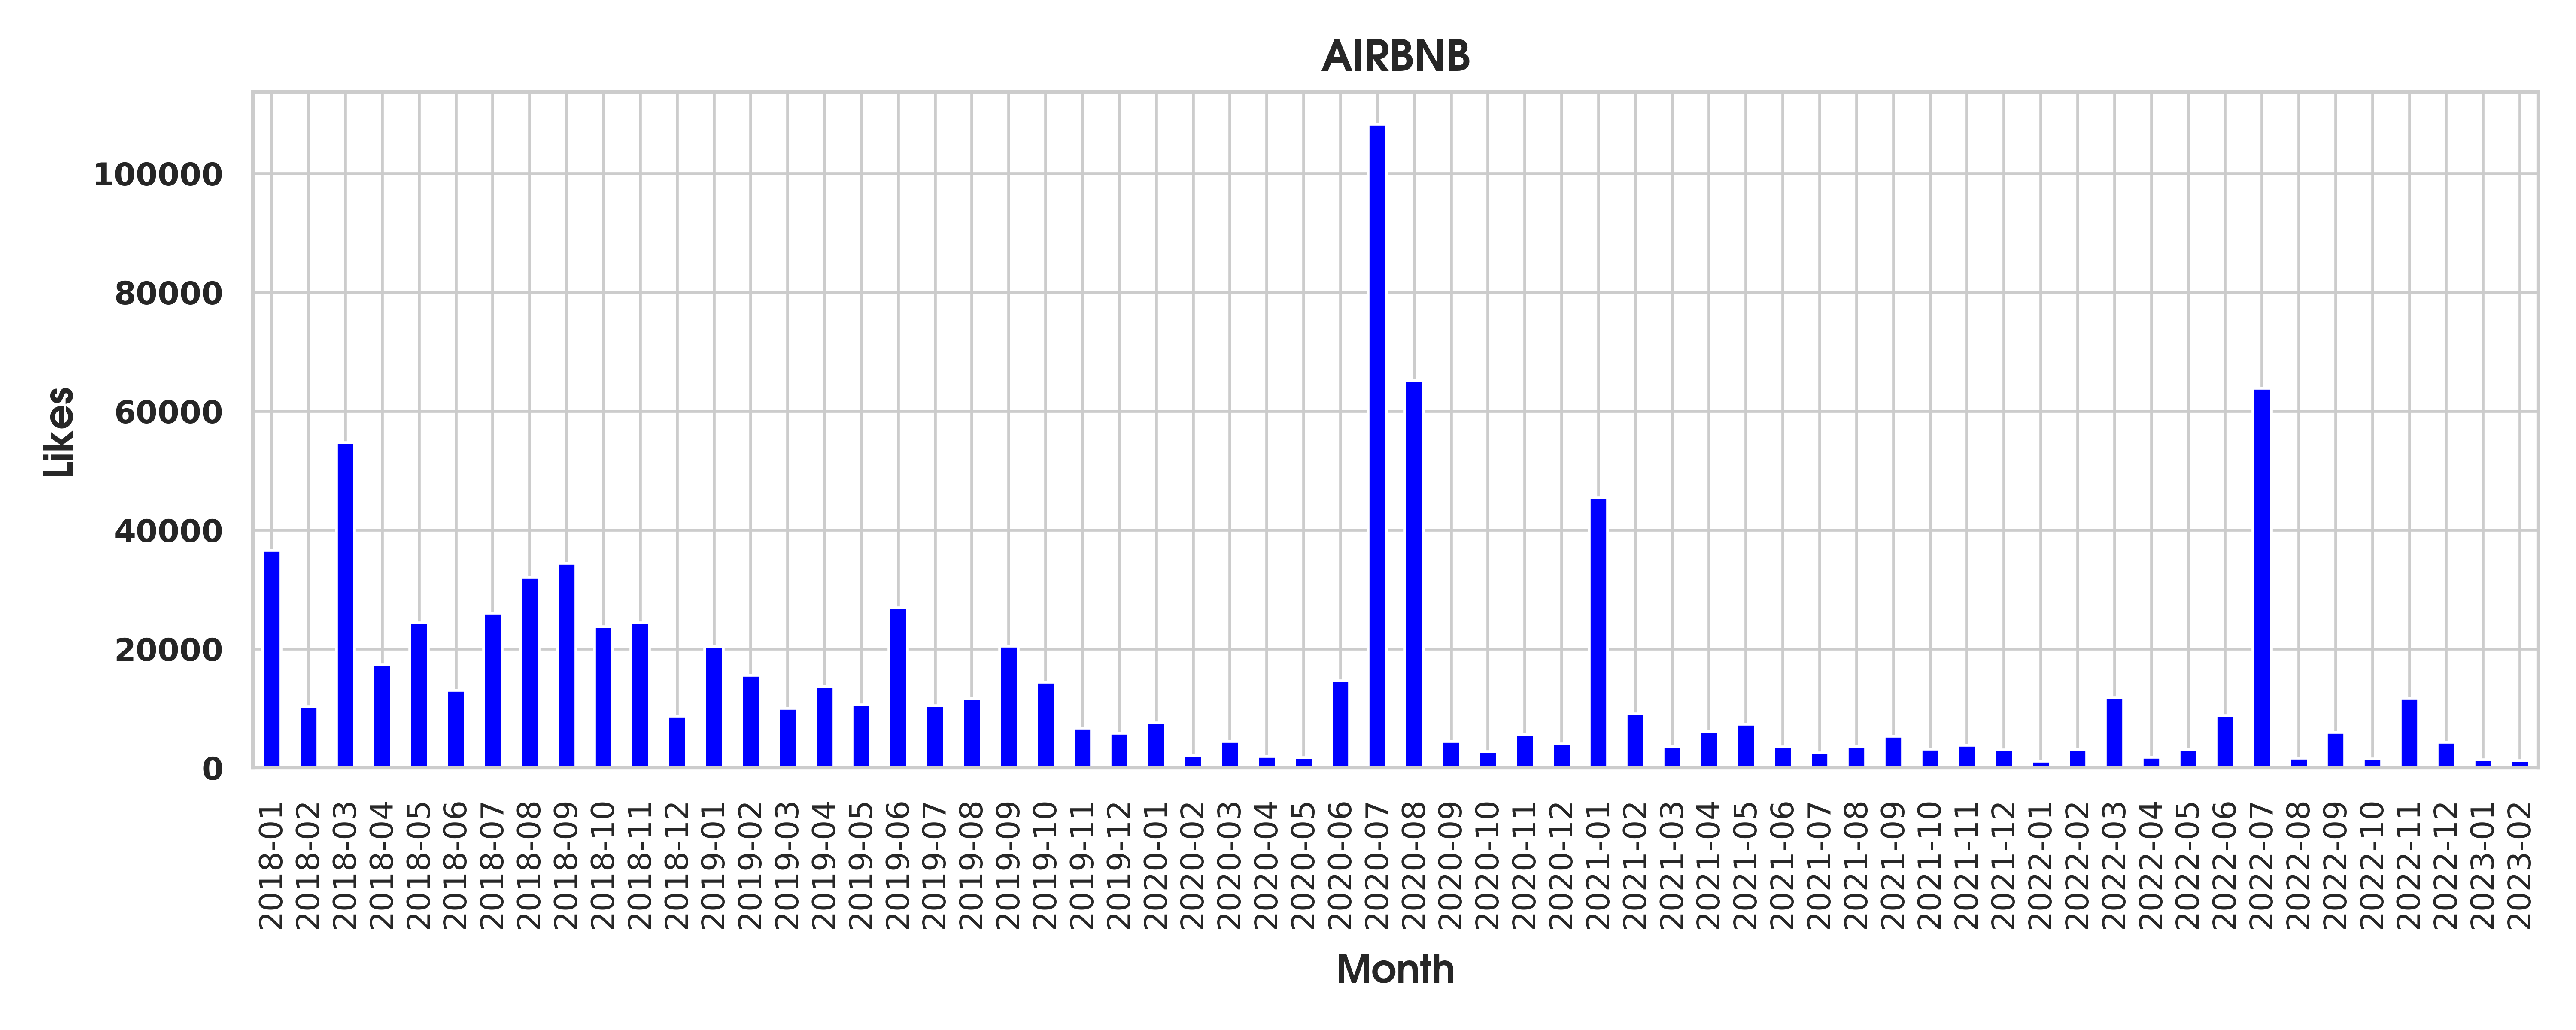
\includegraphics[width=1\textwidth,scale=1]{images/company_tweets_vs_time/airbnb_likes.png}
         \caption{}
    \end{subfigure}
    \begin{subfigure}[b]{0.45\textwidth}
         \centering
         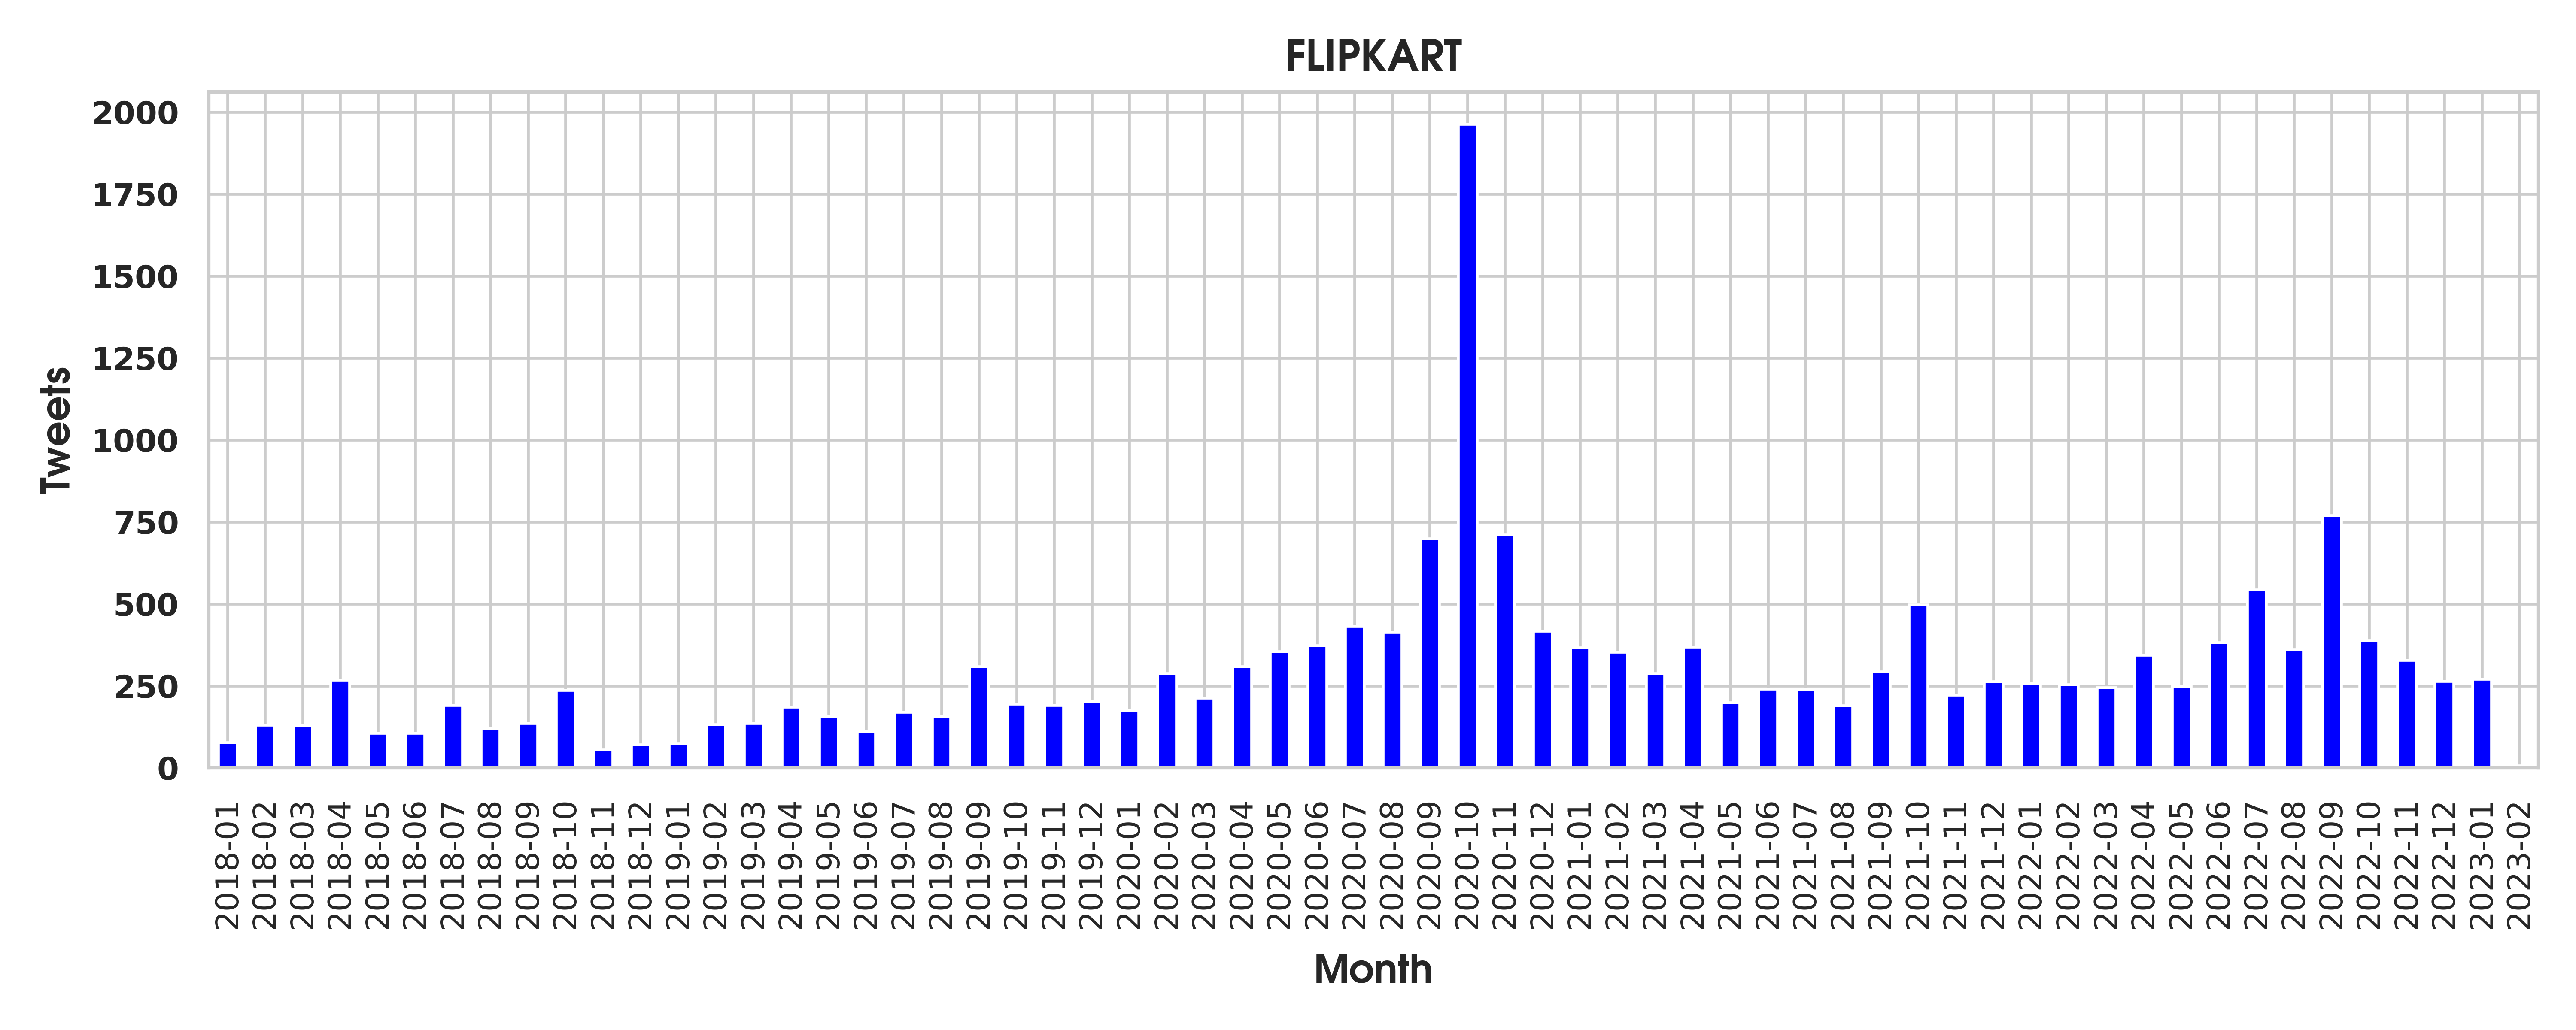
\includegraphics[width=1\textwidth,scale=1]{images/company_tweets_vs_time/flipkart_tweets.png}
         \caption{}
    \end{subfigure}
    \begin{subfigure}[b]{0.45\textwidth}
         \centering
         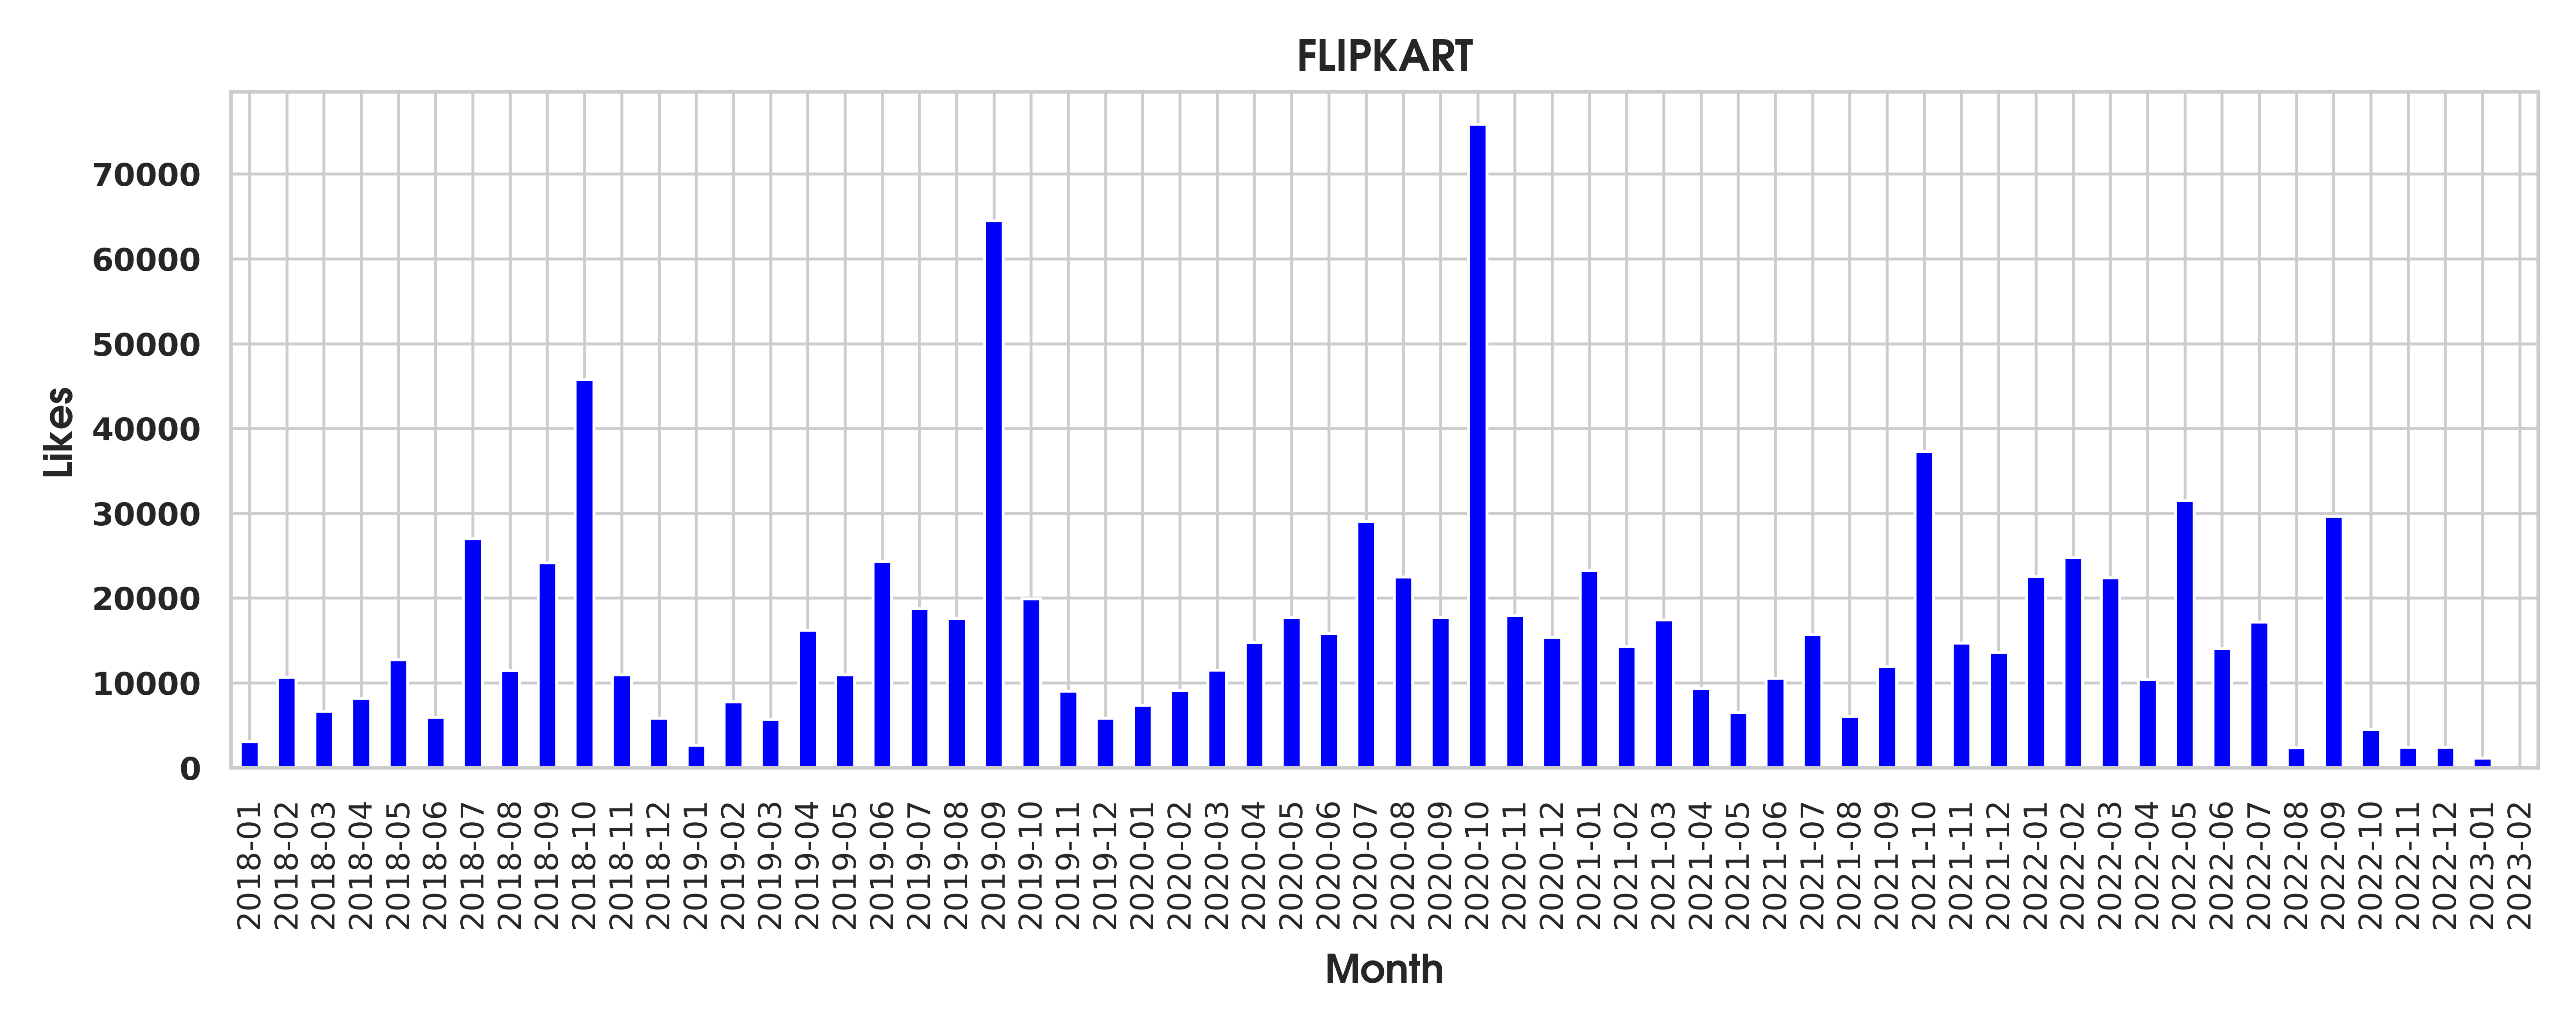
\includegraphics[width=1\columnwidth,scale=1]{images/company_tweets_vs_time/flipkart_likes.png}
         \caption{}
    \end{subfigure}
    % company 3
    \begin{subfigure}[b]{0.45\textwidth}
         \centering
         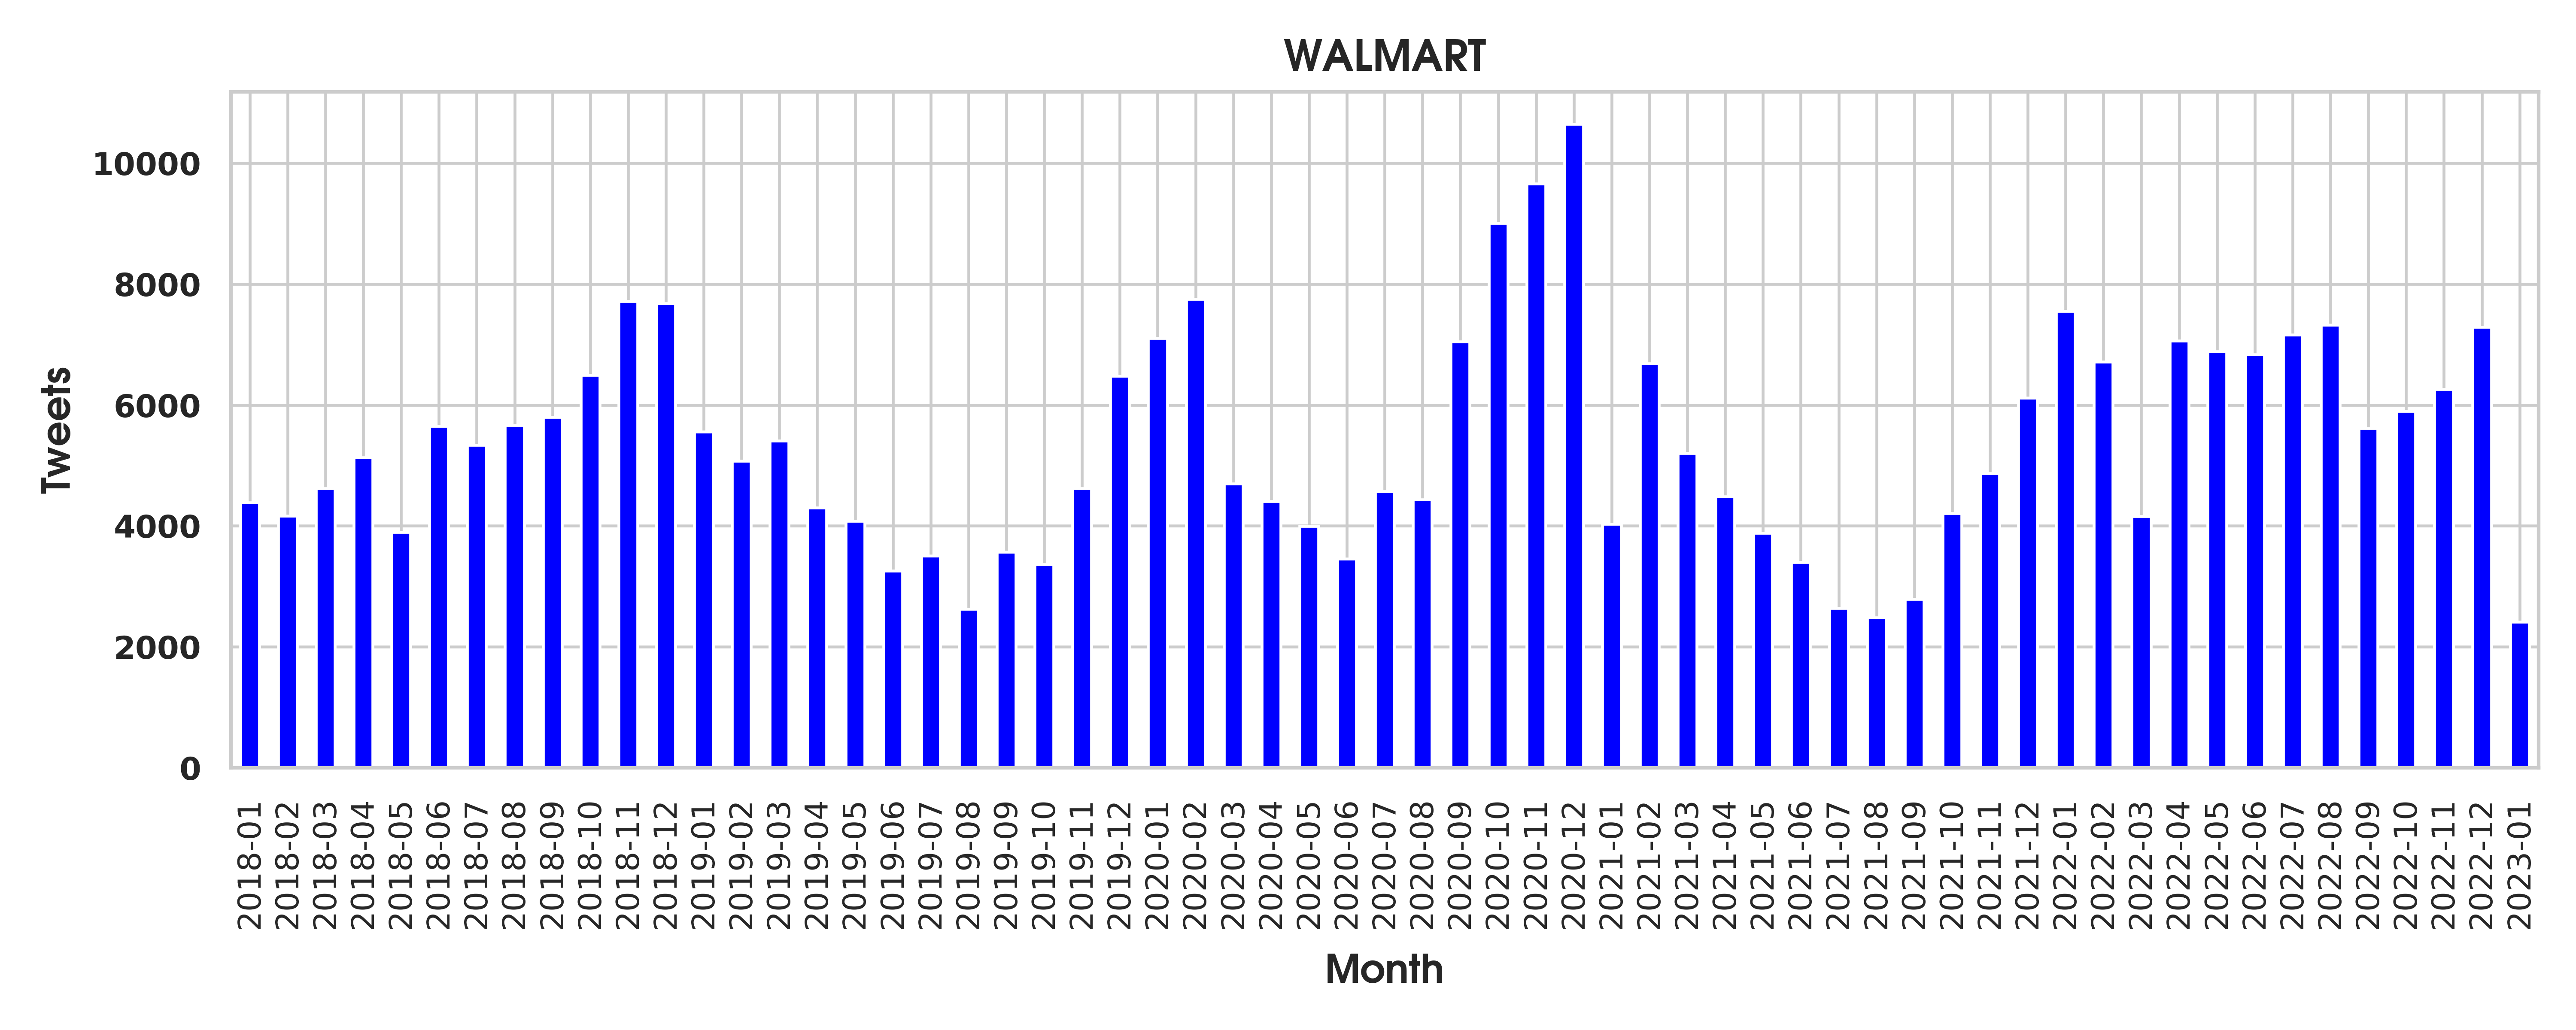
\includegraphics[width=1\columnwidth,scale=1]{images/company_tweets_vs_time/walmart_tweets.png}
         \caption{}
    \end{subfigure}
    \begin{subfigure}[b]{0.45\textwidth}
         \centering
         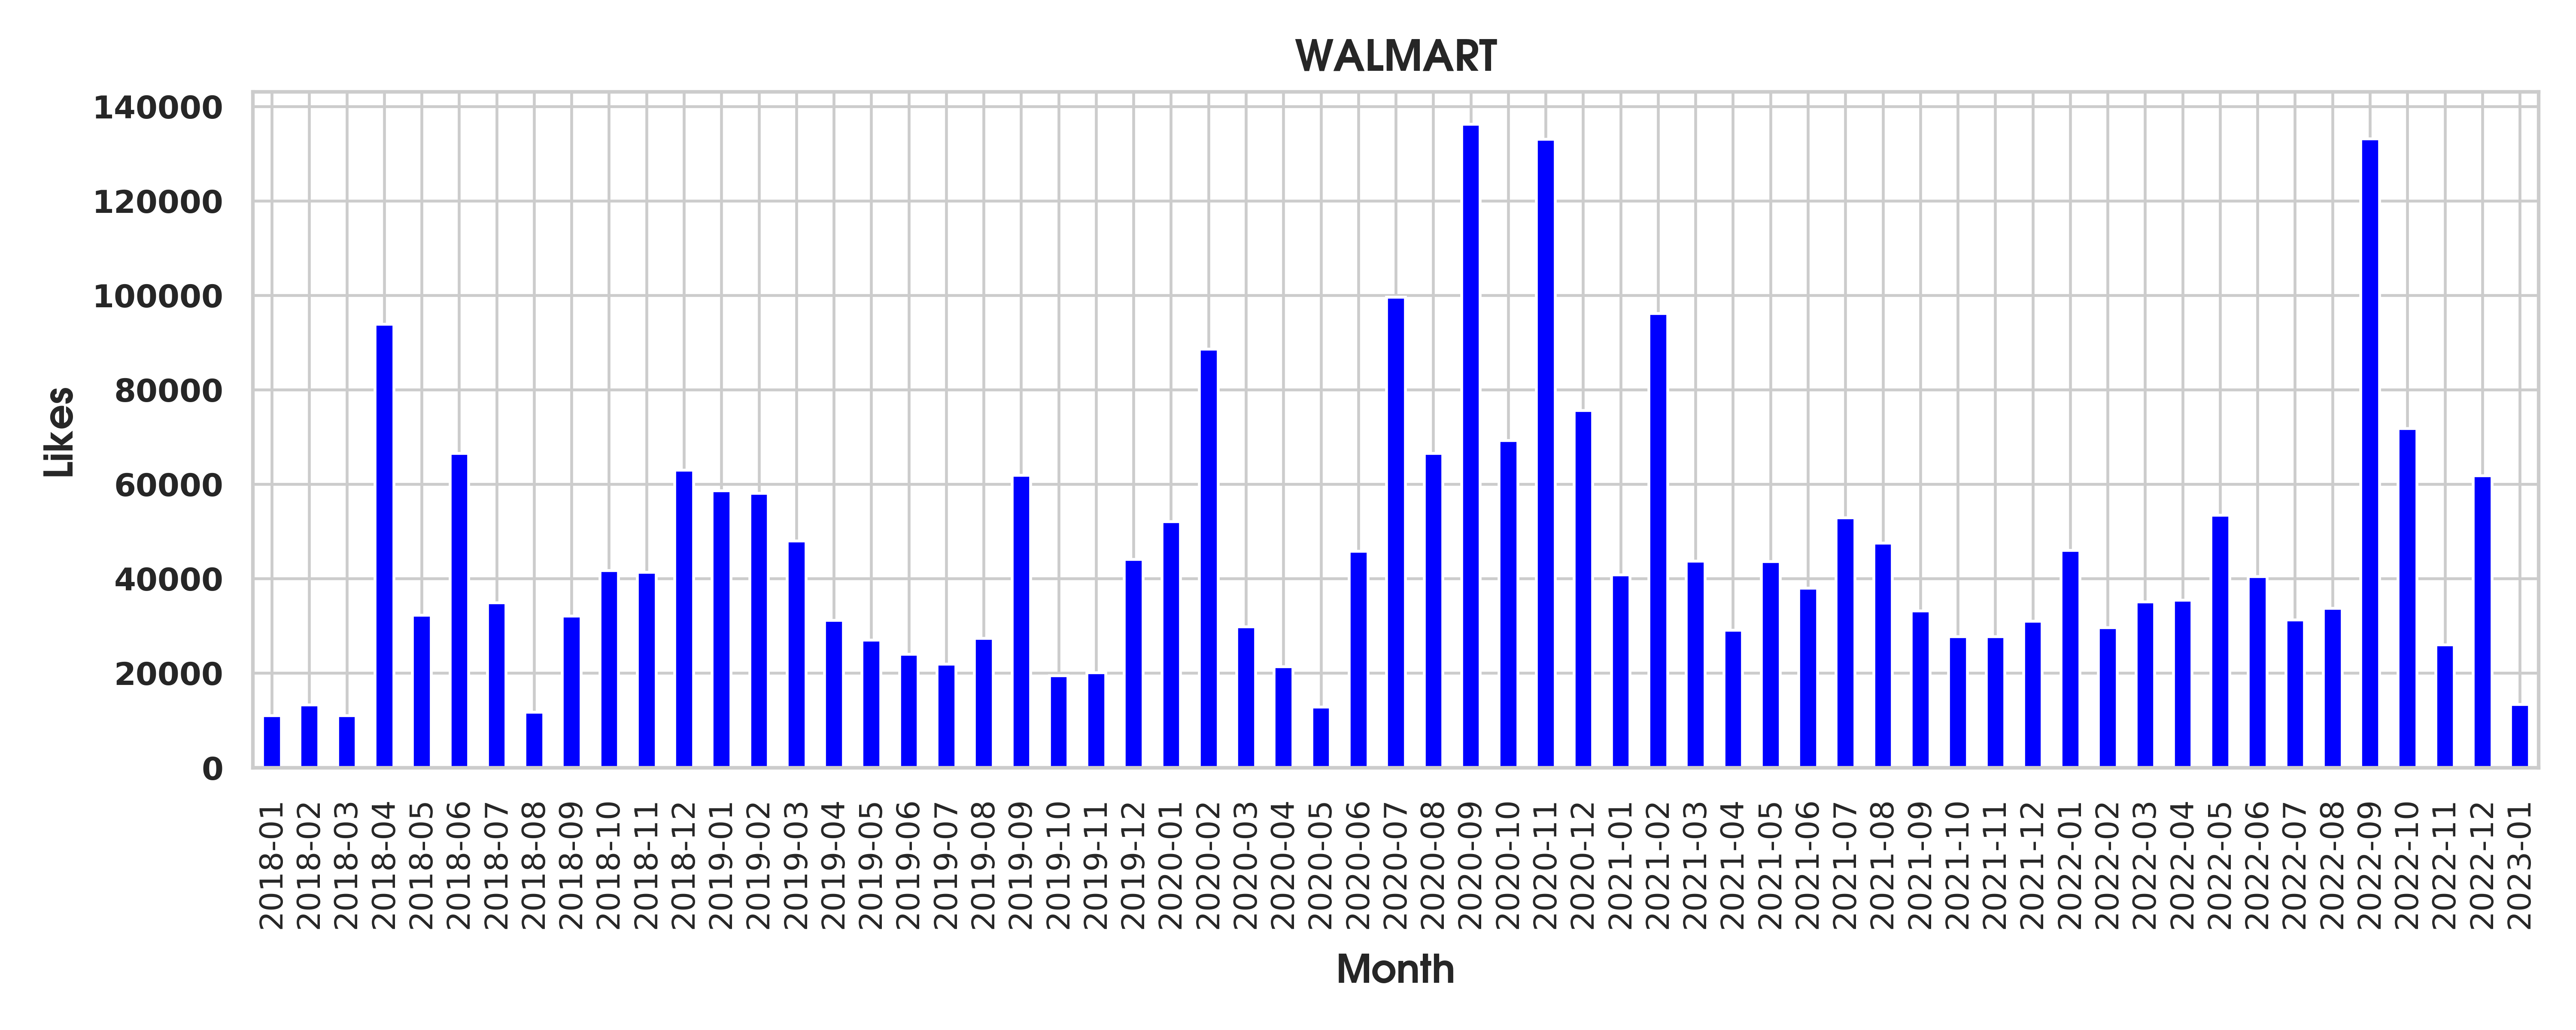
\includegraphics[width=1\columnwidth,scale=1]{images/company_tweets_vs_time/walmart_likes.png}
         \caption{}
    \end{subfigure}
    % company 4
    \begin{subfigure}[b]{0.45\textwidth}
         \centering
         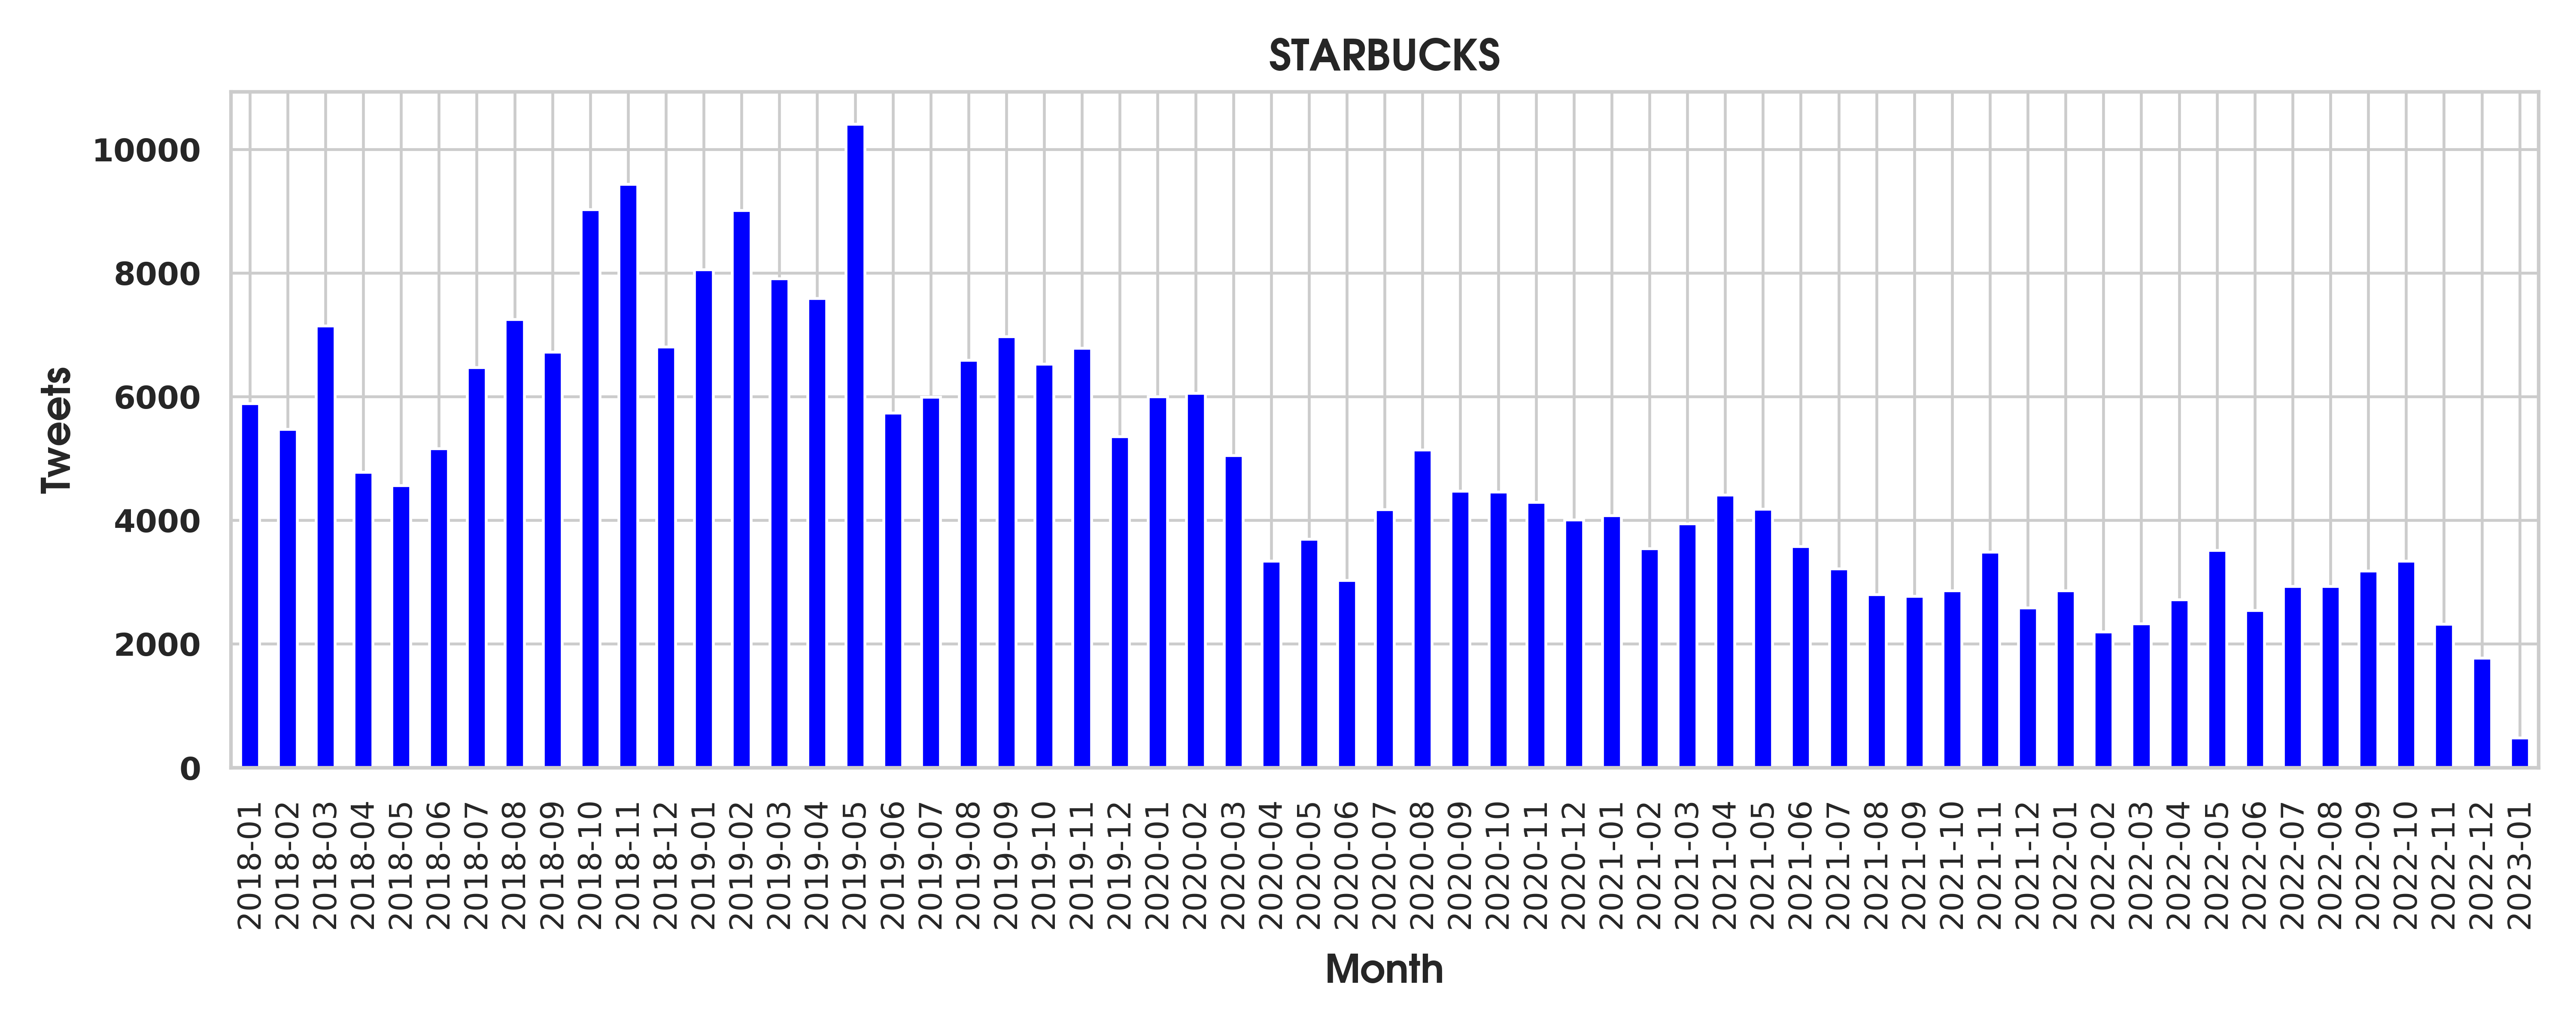
\includegraphics[width=1\columnwidth,scale=1]{images/company_tweets_vs_time/starbucks_tweets.png}
         \caption{}
    \end{subfigure}
    \begin{subfigure}[b]{0.45\textwidth}
         \centering
         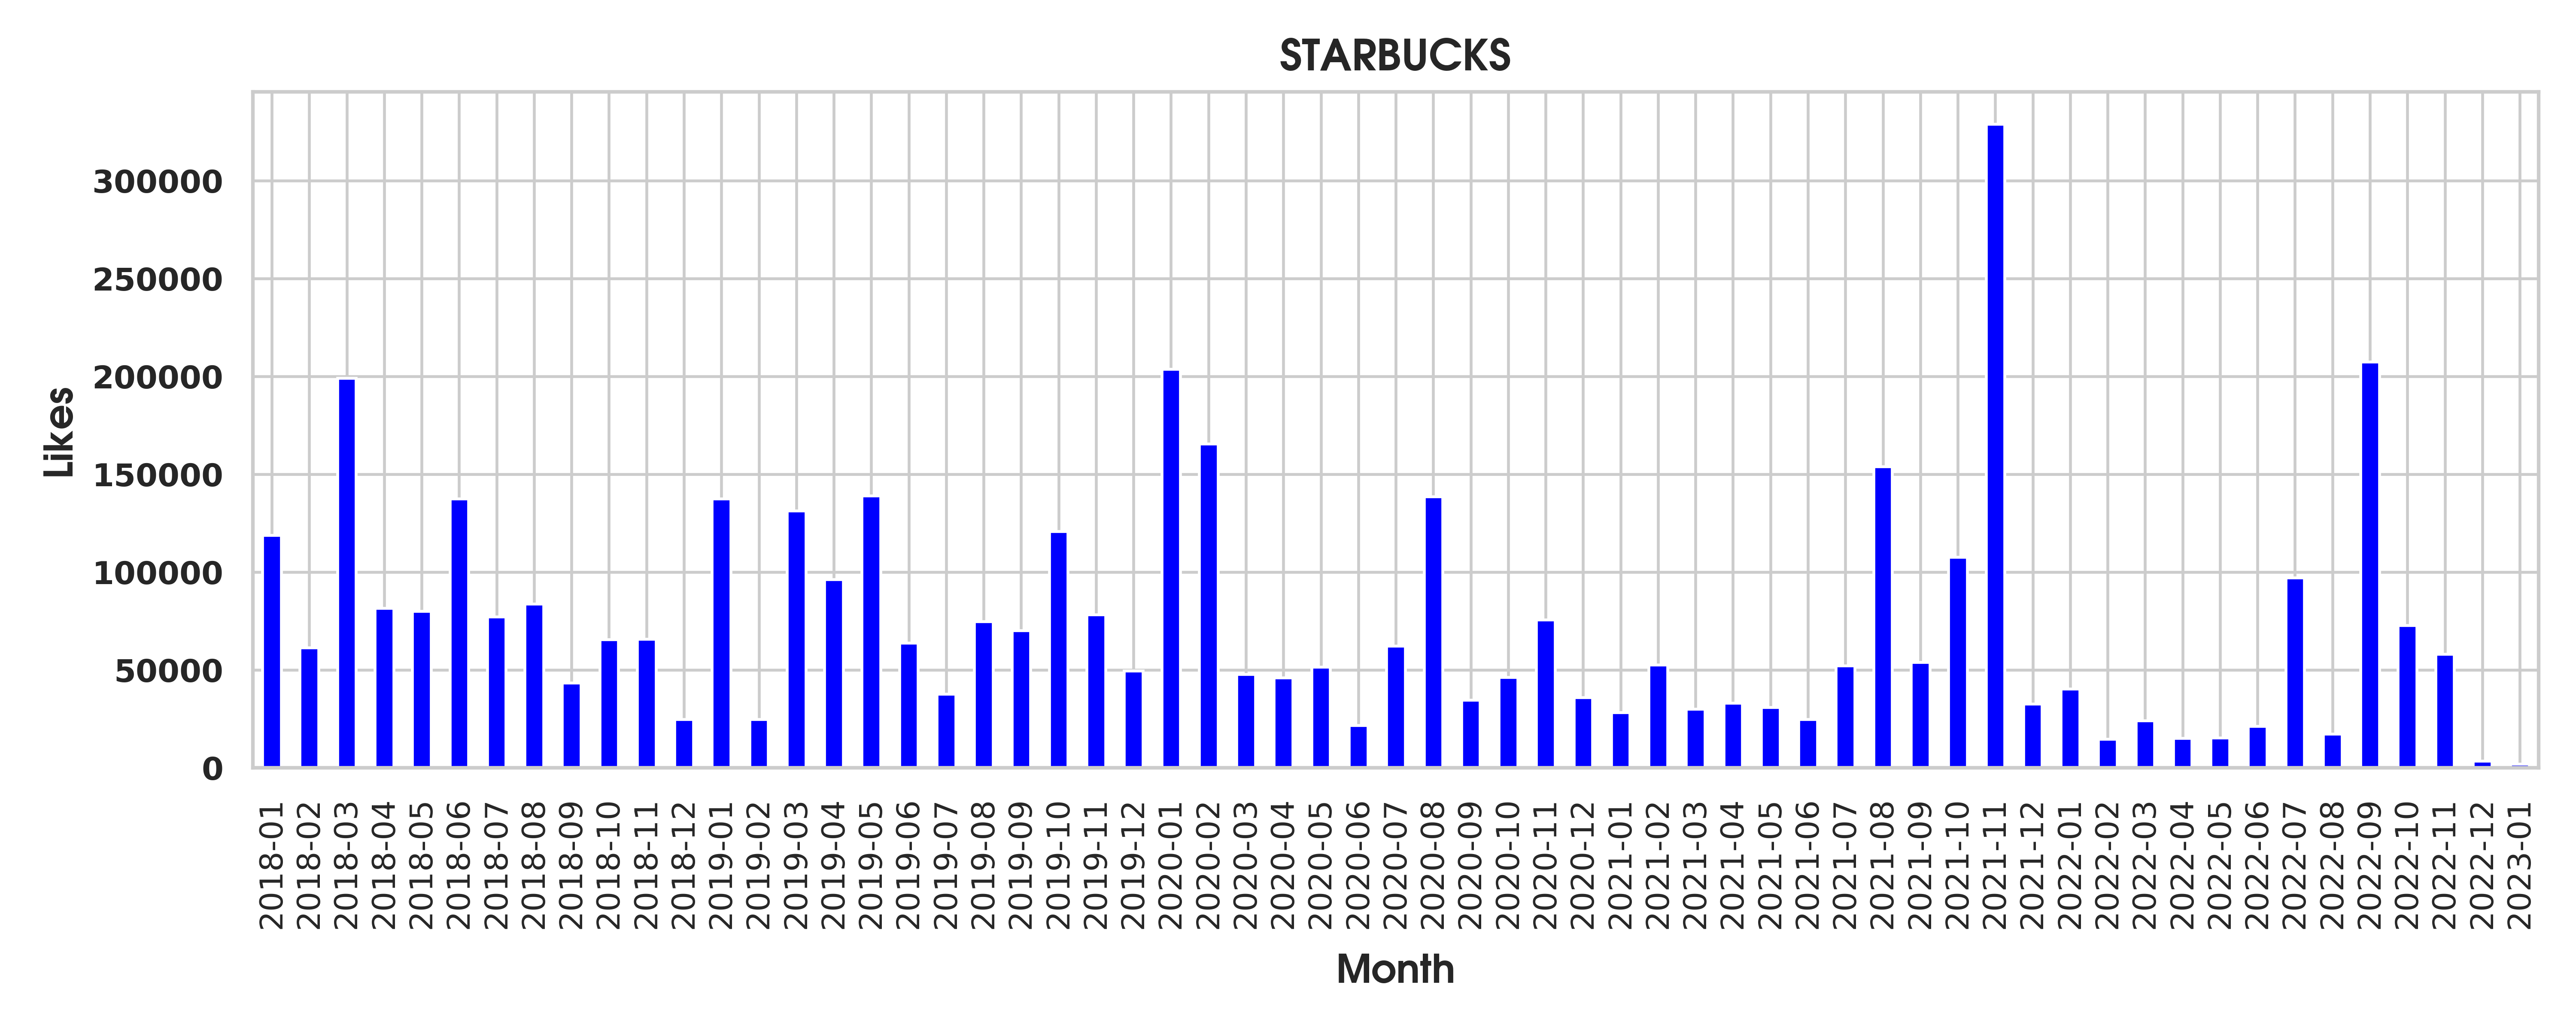
\includegraphics[width=1\columnwidth,scale=1]{images/company_tweets_vs_time/starbucks_likes.png}
         \caption{}
    \end{subfigure}
    % company 5
    \begin{subfigure}[b]{0.45\textwidth}
         \centering
         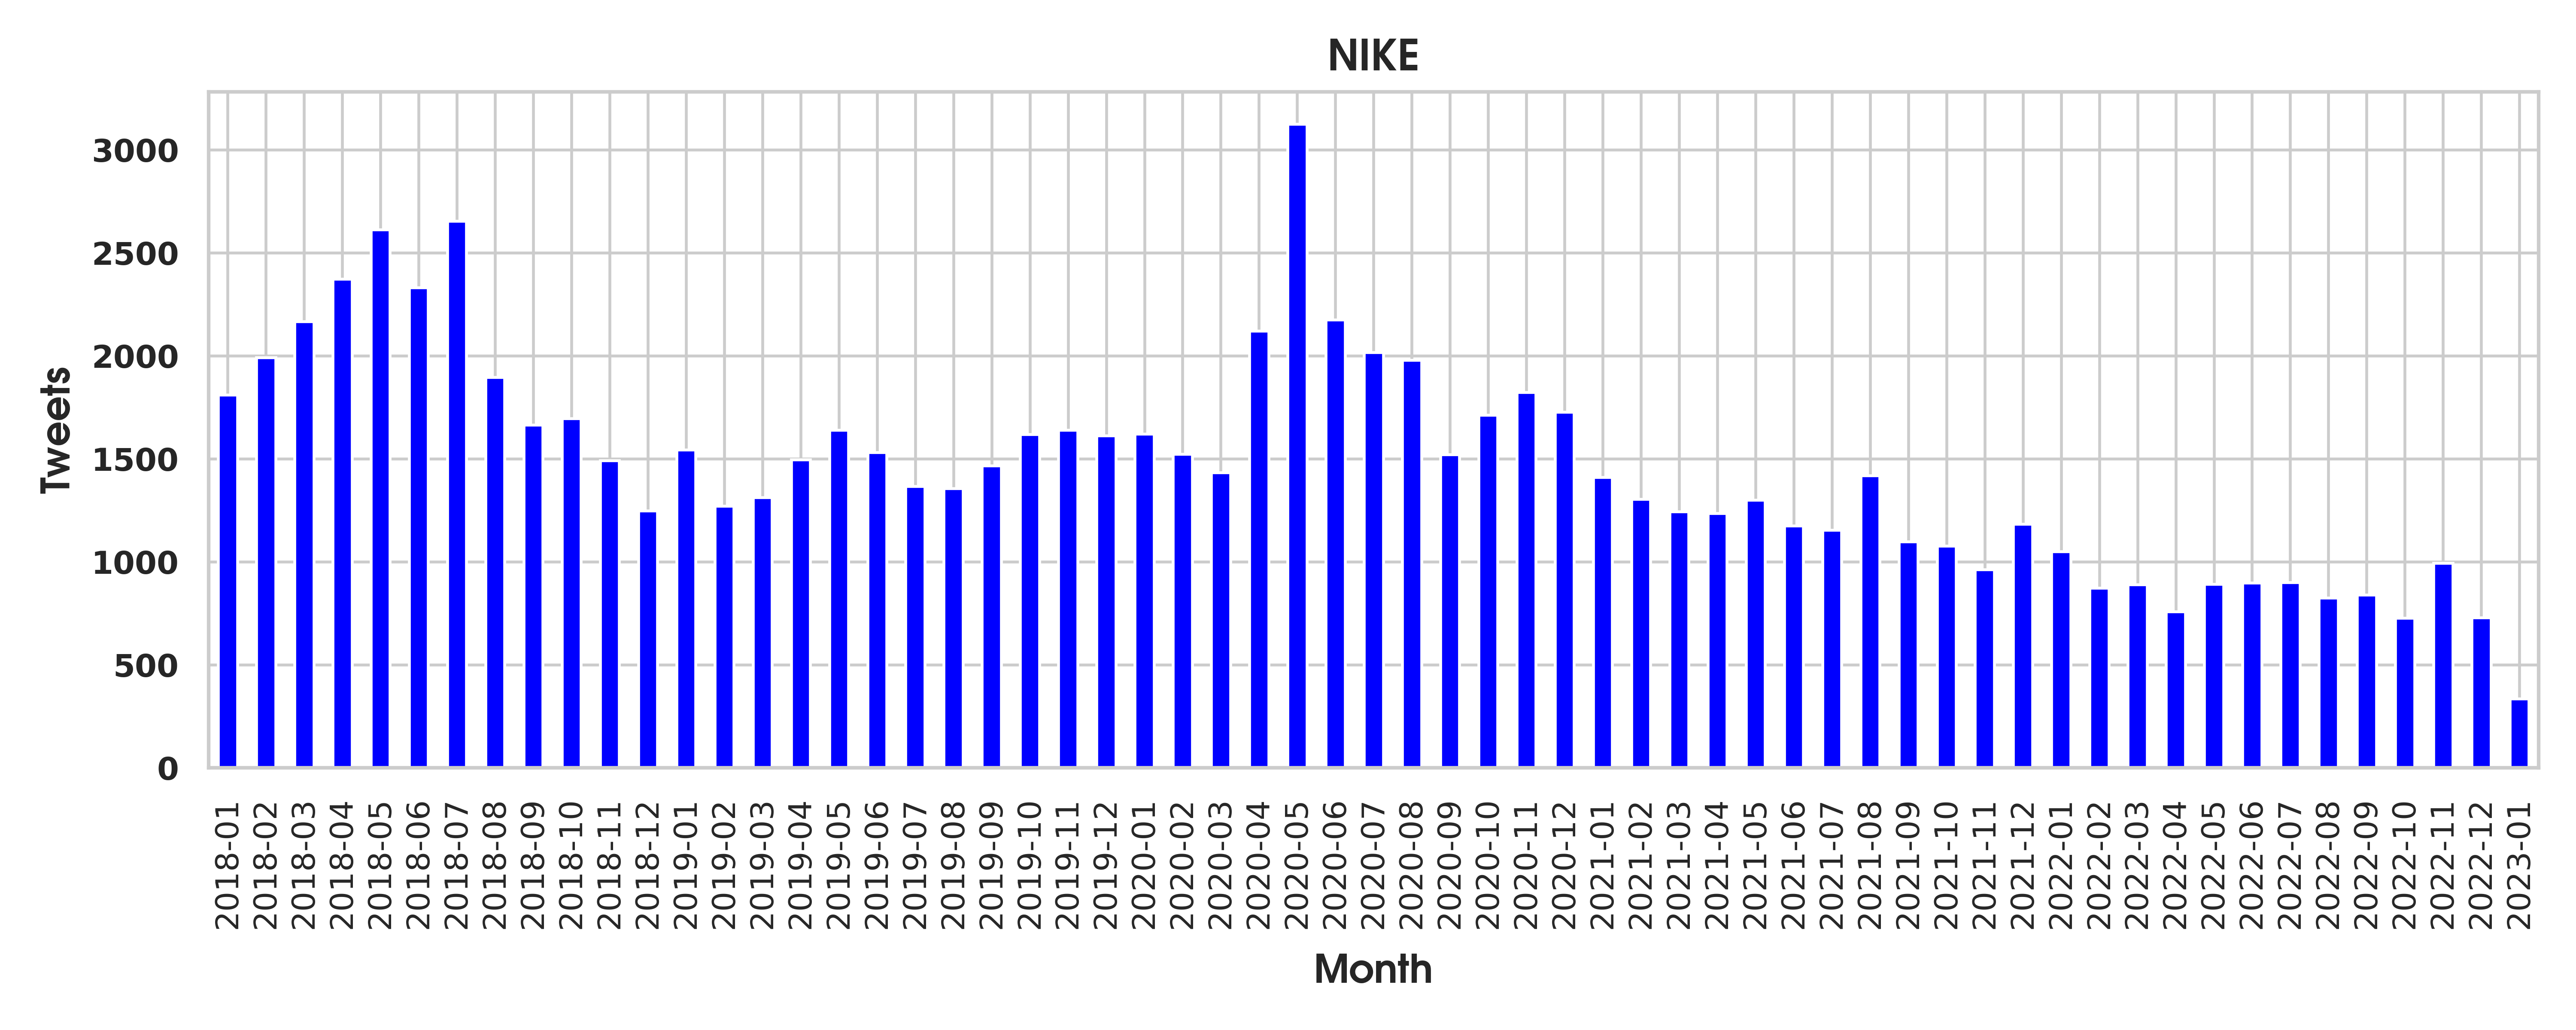
\includegraphics[width=1\columnwidth,scale=1]{images/company_tweets_vs_time/nike_tweets.png}
         \caption{}
    \end{subfigure}
    \begin{subfigure}[b]{0.45\textwidth}
         \centering
         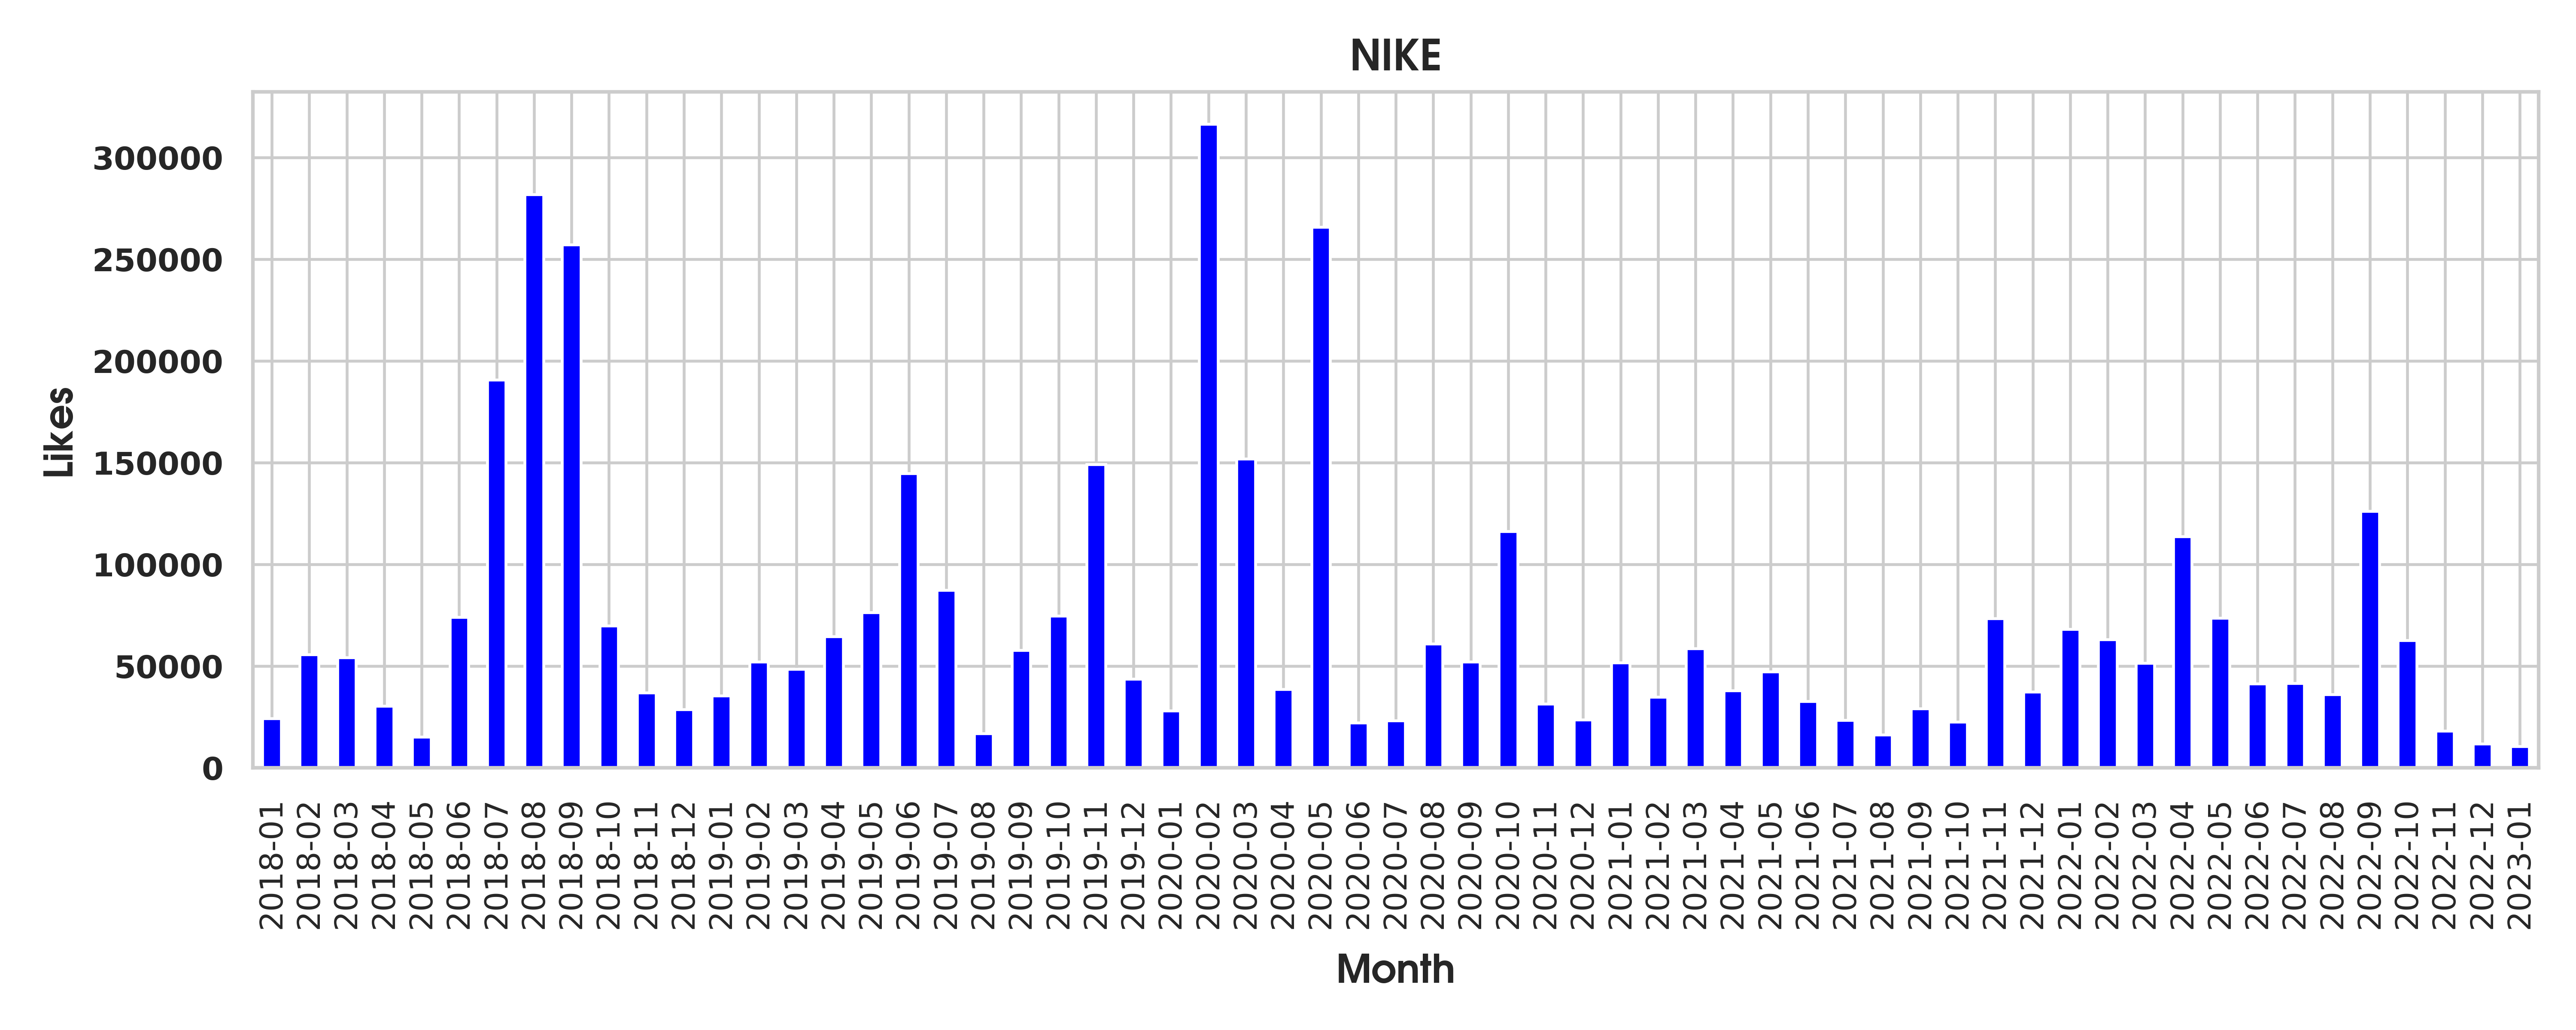
\includegraphics[width=1\columnwidth,scale=1]{images/company_tweets_vs_time/nike_likes.png}
         \caption{}
    \end{subfigure}
   
     \caption{Plots showing variation of number of tweets and likes with time for a few companies in the EngagingImageNet dataset \label{fig:company_tweets_vs_time}}
\end{figure*}


\iffalse
    

\begin{figure*}
  \centering
  \includegraphics[width=1.0\textwidth]{images/Perceptual Analysis.png}
  \caption{Levels of image analysis, motivated by levels of linguistic analysis \cite{} (Fig.~\ref{}). The image lists tasks, and their sample outputs arranged in a hierarchy \cite{shannon-weaver-1949}. Until now, image generation has been optimized primarily on the first two levels of image analysis (Perception and Semantics). A recent work \cite{} looked into optimizing image aesthetics. The last two levels need much more work. In this paper, we work on the behavioral alignment of image generation.}
\end{figure*}



\begin{figure}
  \centering
  \includegraphics[width=1.0\columnwidth]{images/Major_levels_of_linguistic_structure.png}
  \caption{Linguistic Subfields represented as levels of linguistic analysis \cite{wiki-linguistics}. }
\end{figure}

\fi




\subsubsection{Prompts for Instruction Finetuning}
\label{sec:Preparing the Eoig instructions dataset}

\begin{lstlisting}[caption={Visual instruction finetuning Pattern: EngageNet predicts user engagement of images given contextual information about the social media post.},frame=single,label={EngageNet:behaviour_simulation-1},basicstyle=\scriptsize]]

Input: <image>
This is an image that a marketer from company "gucci" wants to post on social media for marketing purposes. The following information about this image is also given:
(1) image resolution i.e. (width, height): [680, 680],
(2) image colors and tones: {"color and tones": {"colors": {"Orange": {"coverage": 0.6}, "White": {"coverage": 0.18}, "Pink": {"coverage": 0.12}, "Brown": {"coverage": 0.1}}, "tones": {"warm": 0.72, "neutral": 0.28, "cool": 0}}},
(3) marketer's intended image description: A girl with a nose ring and gold earrings.,
(4) marketer's intended image tags: nose ring, gold earrings, girl, makeup, lips, face, beauty, earrings, nose, lips, gold, woman, makeup, accessories,
(5) date of posting: 22-February-2019
Now, carefully observe the image. You have to predict the "number of likes" that this image will get, on a scale of 0 to 100. 
It measures the number of times the viewers will interact with the social media post by clicking the "Like" button to express their appreciation for the image. Thus, an image with higher visual appeal, alignment with the company's brand identity, and relevance to the audience, is likely to receive more likes. Moreover, a good image should stongly correspond with the marketer's intended image description and tags to attract the target audience. 
Your predicted "number of likes" will help the marketer to decide whether to post this image or not on the social media platform.
Answer properly in JSON format. Do not include any other information in your answer.

Output:
{"likes": 19}
    
\end{lstlisting}

\begin{lstlisting}[caption={Engagement Finetuning Verbalization Pattern (1): Explicitly asking model to pay attention to engagement tokens},frame=single,label={EngageNet:verbalization-1},basicstyle=\scriptsize]
Input: You are a smart model. I am giving you some data regarding an image - (1) captions (2) keywords (3) image resolution i.e. (width, height) (4) release date (5) number of downloads i.e. how many times the image was downloaded (6) number of forwards i.e. how many times the image was forwarded to someone else (7) number of impressions i.e. how many times the image was seen by someone. Note that (5), (6) and (7) are Key Performance Indicators (KPIs) of the image, thus they are important signals of its perceived quality and popularity.
You have to predict following attributes of the image: (1) colour and tones from the lists given below: - Allowed colours: ['Red', 'Dark_Red', 'Green', 'Bright_Green', 'Dark_Green', 'Light_Green', 'Mud_Green', 'Blue', 'Dark_Blue', 'Light_Blue', 'Royal_Blue', 'Black', 'White', 'Off_White', 'Gray', 'Dark_Gray', 'Silver', 'Cream', 'Magenta', 'Cyan', 'Yellow', 'Mustard', 'Khaki', 'Brown', 'Dark_Brown', 'Violet', 'Pink', 'Dark_Pink', 'Maroon', 'Tan', 'Purple', 'Lavender', 'Turquoise', 'Plum', 'Gold', 'Emerald', 'Orange', 'Beige', 'Lilac', 'Olive']  - Allowed tones: ['warm', 'neutral', 'cool'] (2) main objects present in the image and the diagonal coordinates of their bounding boxes: [x1, y1, x2, y2]
Now, predict the attributes for the following image: [captions: "Waist up portrait of mixed-race female worker posing confidently while standing with arms crossed in plant workshop", keywords: "female, worker, young, woman, mixed-race, african, african-american, modern, contemporary, work, occupation, industry, industrial, plant, factory, workshop, work shop, strong, tough, gritty, masculine, short, hair, latin-american, plump, adult, mechanic, repair, repairman, handywoman, foreman, copy space, portrait, looking at camera, standing, posing, smiling, recruitment, employment, job, opportunity, engineer, production, manufacturing, assembly, assembling, line", image resolution: "(5760, 3840)", release date: "2019-12-02", number of downloads: "24", number of forwards: "106", number of impressions: "5941"] Answer properly in JSON format. Do not include any other information in your answer.

Output: {"color and tones": {"colors": {"Gray": {"coverage": 0.4}, "Dark_Gray": {"coverage": 0.22}, "Black": {"coverage": 0.14}, "Off_White": {"coverage": 0.13}, "Silver": {"coverage": 0.11}}, "tones": {"warm": 0, "neutral": 1.0, "cool": 0}}, "objects": {"jeans": [2076.67, 2542.5, 3023.88, 3827.01], "woman": [1892.94, 11.18, 4260.09, 3824.34], "safety vest": [2160.75, 1410.95, 3668.16, 3826.63], "shirt": [2163.59, 1079.3, 4254.59, 3826.1]}}
\end{lstlisting}


\begin{lstlisting}[caption={Engagement Finetuning Verbalization Pattern (2): Noisy engagement in input and asking the model to correct the noise in addition to producing content},frame=single,label={EngageNet:verbalization-2},basicstyle=\scriptsize]
Input: "You are a smart model. I am giving giving you some data regarding an image released by a content creator - (1) captions (2) keywords (3) image resolution i.e. (width, height) (4) release date (5) approximate number of downloads that the creator wants to achieve (6) approximate number of forwards that the creator wants to achieve (7) approximate number of impressions/views that the creator wants to achieve
You have to predict following attributes of the image: (1) colour and tones from the lists given below: - Allowed colours: ['Red', 'Dark_Red', 'Green', 'Bright_Green', 'Dark_Green', 'Light_Green', 'Mud_Green', 'Blue', 'Dark_Blue', 'Light_Blue', 'Royal_Blue', 'Black', 'White', 'Off_White', 'Gray', 'Dark_Gray', 'Silver', 'Cream', 'Magenta', 'Cyan', 'Yellow', 'Mustard', 'Khaki', 'Brown', 'Dark_Brown', 'Violet', 'Pink', 'Dark_Pink', 'Maroon', 'Tan', 'Purple', 'Lavender', 'Turquoise', 'Plum', 'Gold', 'Emerald', 'Orange', 'Beige', 'Lilac', 'Olive'] - Allowed tones: ['warm', 'neutral', 'cool']  (2) main objects present in the image and the diagonal coordinates of their bounding boxes: [x1, y1, x2, y2]  (3) exact number of downloads that the image will get  (4) exact number of forwards that the image will get  (5) exact number of impressions/views that the image will get
Now, predict the attributes for the following image: [ captions: ""Hispanic adult man holding 100 brazilian real banknotes smiling happy pointing with hand and finger to the side"", keywords: ""pointing, side, face, happy, hopeful, smile, finger, optimistic, hand, point, showing, looking, smiling, one, gesture, confident, up, cheerful, look, mouth, joy, friendly, expression, emotion, presentation, idea, blue, background, hispanic, latin, man, male, guy, beard, bald, shaved, adult, young, money, currency, business, brazilian, cash, brazil, real, investment, banknote, 100"", image resolution: ""(9216, 6144)"", release date: ""2021-02-27"", approximate number of downloads that the creator wants to achieve: ""4"", approximate number of forwards that the creator wants to achieve: ""17"", approximate number of impressions/views that the creator wants to achieve: ""919"" ] Answer properly in JSON format. Do not include any other information in your answer."

Output: {"color and tones": {"colors": {"Cyan": {"coverage": 0.69}, "Light_Blue": {"coverage": 0.16}, "Turquoise": {"coverage": 0.15}}, "tones": {"warm": 0, "neutral": 0, "cool": 1.0}}, "objects": {"man": [1068.6, 18.57, 8143.44, 6121.09], "banknote bill": [3443.5, 2146.79, 5294.15, 3455.05]}, "exact downloads": 4, "exact forwards": 15, "exact impressions": 885}

\end{lstlisting}



\begin{lstlisting}[caption={Engagement Finetuning Verbalization Pattern (3): Noisy engagement in input and asking the model to correct engagement in output},frame=single,label={EngageNet:verbalization-3},basicstyle=\scriptsize]
Input: "You are a smart model. I am giving giving you some data regarding an image released by a content creator - (1) captions (2) keywords (3) image resolution i.e. (width, height) (4) release date (5) approximate number of downloads that the creator wants to achieve (6) approximate number of forwards that the creator wants to achieve (7) approximate number of impressions/views that the creator wants to achieve
You have to predict following attributes of the image: (1) exact number of downloads that the image will get (2) exact number of forwards that the image will get (3) exact number of impressions/views that the image will get.
Now, predict the attributes for the following image: [ captions: ""Movie slapstick vector illustration. Behind the scenes inscription on flapper"", keywords: ""behind the scenes, slapstick, flapper, movie, cinema, scene, logo, frame, film, duration, behind, act, black, cameraman, clip, date, director, entertainment, flap, footage, gray, hollywood, icon, illustration, inscription, operator, screen, shooting, sign, signal, symbol, television, theater, time, timecode, tv, vector, video, view, white"", image resolution: ""(4096, 4096)"", release date: ""2017-06-11"", approximate number of downloads that the creator wants to achieve: ""5"", approximate number of forwards that the creator wants to achieve: ""31"", approximate number of impressions/views that the creator wants to achieve: ""914"" ] Answer properly in JSON format. Do not include any other information in your answer. "

Output: {"exact downloads": 5, "exact forwards": 32, "exact impressions": 864}
\end{lstlisting}




\begin{lstlisting}[caption={Engagement Finetuning Verbalization Pattern (4): No engagement in input and asking the model to simulate exact engagement in output},frame=single,label={EngageNet:verbalization-4},basicstyle=\scriptsize]
Input: "You are a smart model. I am giving giving you some data regarding an image released by a content creator - (1) captions (2) keywords (3) image resolution i.e. (width, height) (4) release date
You have to predict following attributes of the image: (1) exact number of downloads that the image will get (2) exact number of forwards that the image will get (3) exact number of impressions/views that the image will get
Now, predict the attributes for the following image: [captions: ""Company employees working in software development and designer office"", keywords: ""business, office, meeting, collaegue, successful, workplace, analysis, architect, coworker, discussion, entrepreneur, marketing, professional, company, employee, occupation, software, work, worker, team, people, brainstorming, cooperation, corporate, project, strategy, teamwork, together, computer, colleagues, young, diverse, collaboration, design, developer, group, ideas, management, smiling, multiethnic, place, plan, research, startup, technology, women, programmer, architects"", image resolution: ""(4035, 2690)"", release date: ""2020-09-29"" ]. Answer properly in JSON format. Do not include any other information in your answer."

Output: {"exact downloads": 1, "exact forwards": 1, "exact impressions": 186}
\end{lstlisting}

%%%%%%%%%%%%%%
% Listings format - black box
% \tcbset{colback=black!5,colframe=black!80,coltitle=white,width=\textwidth,box align=top,label={sample_color_box}}

%%%%%%%%%%% PROMPT - 1: VIFT OF EngageNet
% \begin{tcolorbox}[title=\small{Engagement-aware visual instruction finetuning Pattern: EngageNet predicts user engagement of images given contextual information about the social media post}]
% \scriptsize{
% \textbf{Input:} <image>
% This is an image that a marketer from company "gucci" wants to post on social media for marketing purposes. The following information about this image is also given:
% (1) image resolution i.e. (width, height): [680, 680],
% (2) image colors and tones: {"color and tones": {"colors": {"Orange": {"coverage": 0.6}, "White": {"coverage": 0.18}, "Pink": {"coverage": 0.12}, "Brown": {"coverage": 0.1}}, "tones": {"warm": 0.72, "neutral": 0.28, "cool": 0}}},
% (3) marketer's intended image description: A girl with a nose ring and gold earrings.,
% (4) marketer's intended image tags: nose ring, gold earrings, girl, makeup, lips, face, beauty, earrings, nose, lips, gold, woman, makeup, accessories,
% (5) date of posting: 22-February-2019
% Now, carefully observe the image. You have to predict the "number of likes" that this image will get, on a scale of 0 to 100. 
% It measures the number of times the viewers will interact with the social media post by clicking the "Like" button to express their appreciation for the image. Thus, an image with higher visual appeal, alignment with the company's brand identity, and relevance to the audience, is likely to receive more likes. Moreover, a good image should stongly correspond with the marketer's intended image description and tags to attract the target audience. 
% Your predicted "number of likes" will help the marketer to decide whether to post this image or not on the social media platform.
% Answer properly in JSON format. Do not include any other information in your answer.

% \textbf{Output:} \{"likes": 19\}
% }
% \end{tcolorbox}



%%%%%%%%%%%%%%%%%%%%%%%%%%%%%%%%%%

Hyperparameters for visual instruction finetuning of EngageNet: 
\begin{itemize}
    \item per device train batch size: 16
    \item gradient accumulation steps: 1
    \item max context length: 2048
    \item warmup ratio: 0.03
    \item warmup learning rate scheduler: cosine
    \item after warmup, learning rate: 2e-5
\end{itemize}



%%%%%%%%%%%%%%%%%%%%%%%%%%%%%%%%%%%%%%%%%%%%%%%%%




\subsubsection{Repurposing EngageNet for Design Specification Generation (DSG)}
\label{sec:EngageNet Content Simulation}

\paragraph{Training For Design Specification Prediction Task}
Prior works \cite{bhattacharya2023video} have demonstrated the capability of language-only pre-trained models like GPT-3 and Vicuna to infer information about visual content without explicit visual reasoning training. Recent models such as BLIP \cite{li2023blip2}, Llava \cite{liu2023visual}, MiniGPT-4 \cite{zhu2023minigpt}, and GPT-4 \cite{openai2023gpt4} have shown language models' ability to 'see' by incorporating visual branches (often a combination of ViT \cite{dosovitskiy2020image} and Qformer \cite{li2023blip2}) and training them with image-language instructions to answer image-related questions. 
However, our findings (Table~\ref{tab:twitter_EngagingImageNet_data_Eoig_llm_results}) reveal that neither pretraining nor further instruction tuning gives a language model the ability to simulate the downstream engagement of an image-based communication or reason about how a more engaging image should look like. Further, we also find that in-context learning, while successful in many other domains, does not perform well in engagement-related tasks. Therefore, to teach a language model about image content and downstream performance, we further train the Llama LLM.

To teach Llama about an image and its downstream engagement, we perform engagement fine-tuning \cite{khandelwal2023large}. We design four types of engagement-finetuning instructions (Listings~\ref{EngageNet:verbalization-1}-\ref{EngageNet:verbalization-4}). The idea is to \textit{verbalize} an image using image perception models like color extractor, tones extractor, object, and coordinate detector and convert it to natural language. Then, the image caption, keywords, the required engagement level, date, and marketer information is fed as input to the LLM and asked to output the image verbalization. This way, the LLM learns to map the image prompt and engagement level to image verbalization.

We train the LLM on the train set of EngagingImageNet data. In Listings~\ref{EngageNet:verbalization-1}-\ref{EngageNet:verbalization-2}, we provide the image caption, keywords, date, and required engagement level as inputs to the model. Our aim is to train the model to predict a design specification comprising colors and tones with their spatial coverage as well as objects with their bounding boxes, that should be reflected in the image. Moreover, we observe improved learning in the language model for engagement-conditioned image generation when introducing a 20\% noise in the engagement. We then task the model to rectify this noise in the output, simultaneously generating the verbalization of the engagement-conditioned image in Listings~\ref{EngageNet:verbalization-3}-\ref{EngageNet:verbalization-4}.





 
 %%%%%%%%%%%%%%%%%%%%%%%%%%%%%%
 % Old reward model - Eoig CS Reward results

 \begin{landscape}
      \begin{table*}\centering
     \caption{
     Performance of all models on the engagement-optimized design specification generation (DSG) task across different engagement-level images in EngagingImageNet data. It is noteworthy that (i)~EngageNet outperforms larger sized GPT-3.5, 4 and also the sized Llama model fine-tuned on the same data (without including engagement tokens). (ii)~In-context learning does not work well in the engagement-conditioned design specification generation domain. 
     % Best results are given in \valbest{green} and runner-ups in \valgood{blue}.
     }\label{tab:twitter_EngagingImageNet_data_Eoig_llm_results}
     % \scriptsize
     \resizebox{1.5\textwidth}{!}{
     \begin{tabular}{c|c|c|cccc|c|ccccc}\toprule
     \multicolumn{12}{c}{\textbf{EngagingImageNet Data}}\\\toprule
     \multirow{2}{*}{\textbf{Model}}  & \multirow{2}{*}{\textbf{\makecell{Engagement\\Optimized}}} &\multirow{2}{*}{\textbf{KPI}} &\multicolumn{4}{c|}{\textbf{Colours}} &\textbf{Tones} &\multicolumn{4}{c}{\textbf{Objects}} \\\cmidrule{4-12}
     & & &\textbf{IOU} $\uparrow$ &\textbf{\makecell{Cosine\\Similarity}} $\uparrow$ &\textbf{\makecell{RGB\\distance}} $\downarrow$ &\textbf{\makecell{Coverage\\RMSE}} $\downarrow$ &\textbf{\makecell{Coverage\\RMSE}} $\downarrow$ &\textbf{IOU} $\uparrow$ &\textbf{\makecell{Cosine\\Similarity}} $\uparrow$ &\textbf{\makecell{Normalised\\Area RMSE}} $\downarrow$ &\textbf{\makecell{Relative\\Position Error}} $\downarrow$ \\\midrule
     \multirow{2}{*}{\makecell{Finetuned\\Llama}} & \multirow{2}{*}{No} &High &\valgood{0.3717} &\valgood{0.8725} &0.2855 &\valgood{0.1694} &\valgood{0.1957} &\valgood{0.2547} &\valgood{0.8071} &\valgood{0.2612} &\valgood{0.3078} \\
     &&Low &\valgood{0.3362} &\valgood{0.8602} &0.2223 &\valgood{0.1811} &\valgood{0.2339} &\valgood{0.2743} &\valgood{0.8047} &\valgood{0.2421} &\valgood{0.2954} \\
     \midrule
     \multirow{2}{*}{\makecell{Finetuned\\Llama (EngageNet)}} & \multirow{2}{*}{\makecell{Engagement\\Finetuning}} &High &\valbest{0.4065} &\valbest{0.8898} &0.2795 &\valbest{0.1507} &\valbest{0.1718} &\valbest{0.2732} &\valbest{0.8122} &\valbest{0.2509} &\valbest{0.3054} \\
     &&Low &\valbest{0.4531} &\valbest{0.8791} &\valbest{0.2084} &\valbest{0.1443} &\valbest{0.1848} &\valbest{0.3455} &\valbest{0.8228} &\valbest{0.2373} &\valbest{0.2889} \\\midrule
     \multirow{2}{*}{3-shot GPT-3.5} &\multirow{2}{*}{\makecell{In-context\\learning}} &High &0.214 &0.7765 &0.2851 &0.1773 &0.396 &0.1085 &0.6621 &0.3090 &0.3651 \\
     &&Low&0.2175 &0.7781 &0.2254 &0.2118 &0.3347 &0.1338 &0.6749 &0.3098 &0.3573 \\\midrule
     \multirow{2}{*}{5-shot GPT-3.5} &\multirow{2}{*}{\makecell{In-context\\learning}} &High &0.2137 &0.7704 &0.2743 &0.1976 &0.324 &0.1011 &0.6456 &0.3160 &0.3622 \\
     &&Low&0.2191 &0.7705 &\valgood{0.2176} &0.2449 &0.3186 &0.1264 &0.656 &0.3150 &0.3615 \\\midrule
     \multirow{2}{*}{3-shot GPT-4} &\multirow{2}{*}{\makecell{In-context\\learning}} &High  &0.2421 &0.7887 &\valgood{0.2726} &0.192 &0.304 &0.1035 &0.6316 &0.3137 &0.3666 \\
     &&Low&0.2405 &0.793 &0.2332 &0.2094 &0.3037 &0.1419 &0.6604 &0.3248 &0.3763 \\\midrule
     \multirow{2}{*}{5-shot GPT-4} &\multirow{2}{*}{\makecell{In-context\\learning}} &High &0.2437 &0.7905 &\valbest{0.2702} &0.1864 &0.2937 &0.1008 &0.6136 &0.3111 &0.3782 \\
     &&Low&0.2448 &0.7924 &0.2278 &0.2144 &0.2944 &0.1464 &0.6406 &0.3301 &0.3857 \\
     \bottomrule
     \end{tabular}}
     \end{table*}
 \end{landscape}
     
     
     %%%%%%%%%%%%%%%%%%%%%%%%%%%%%%%%%%%%%%%%%%%%%%%%%







\paragraph{Results for Engagement-conditioned Design Specification Prediction Task}
 To generate engagement-conditioned image verbalization, we compare several models: in-context trained GPT-3.5 and GPT-4, engagement-finetuned Llama (EngageNet), and Llama fine-tuned on image verbalization but without user engagement information. By comparing against a fine-tuned Llama trained on the same instruction as EngageNet, except with the inclusion of engagement tokens, we aim to isolate the impact of engagement tokens on improving generated engagement-conditioned image verbalizations, independent of the instruction tuning process. We assess all models across multiple metrics that evaluate the extent to which the generated verbalizations align with ground truth in terms of colors, tones, objects, and their positions. Intersection over Union (IoU) metrics gauge the overlap between ground truth and generated constructs (colors and objects), while similarity metrics measure cosine similarity between ground truth and generated constructs (colors, objects). Coverage errors determine the how closely the proportion of ground truth and predicted constructs (colors, tones) in the image match. Additionally, we calculate differences in predicted and ground truth areas and locations for objects, accounting for semantically similar objects (such as sofa and couch). Further details on these metrics and their formulas can be found in Appendix~\ref{sec:Evaluation Metrics}.
 
 
 Table~\ref{tab:twitter_EngagingImageNet_data_Eoig_llm_results} displays the outcomes. The results indicate that engagement fine-tuning enables EngageNet to achieve superior performance across all metrics, surpassing both equivalently sized fine-tuned Llama and 10x larger instruction-tuned GPT-3.5 and GPT-4. 
 % Notably, Medium and Low liked test samples exhibit more substantial improvements compared to the High liked samples, despite the latter having a slightly higher quantity. 
 Furthermore, in-context learning demonstrates subpar performance, with both the three and five-shot models displaying similar results.




\paragraph{Evaluation Metrics for Design Specification Prediction}
\label{sec:Evaluation Metrics}
\begin{itemize}
    \item \textbf{Colours IOU}: The intersection over union between set $C^G$ of colours in the ground truth image verbalization and set $C^P$ of colours in the predicted image verbalization is computed as:
    \begin{equation}
        IOU(C^G, C^P) = \frac{|C^G \cap C^P|}{|C^G \cup C^P|}
    \end{equation}
    \item \textbf{Colours similarity}: For the ground truth colour set $C^G = {c_1^G, c_2^G, ..., c_i^G}$ and predicted colour set $C^P = \{c_1^P, c_2^P, ..., c_j^P\}$, we correspondingly obtain the sets of word vectors $W^G = \{w_1^G, w_2^G, ..., w_i^G\}$ and $W^P = \{w_1^P, w_2^P, ..., w_j^P\}$, using Spacy \footnote{\url{https://spacy.io/}}. For some similarity threshold $\tau$, the mean cosine similarity is computed as follows:
    \begin{equation}
        \frac{\mathop{\sum_{i=1}^{|C^G|}\sum_{j=1}^{|C^P|}} cos(w_i^G, w_j^P).I(w_i^G, w_j^P, \tau)}{\mathop{\sum_{i=1}^{|C^G|}\sum_{j=1}^{|C^P|}} I(w_i^G, w_j^P, \tau) }
    \end{equation}
    where $I(w_i^G, w_j^P, \tau)$ is an indicator function defined as:
    \begin{equation}
        I(w_i^G, w_j^P, \tau) =
    \begin{cases}
        1 & \text{if } cos(w_i^G, w_j^P) > \tau\\
        0 & \text{otherwise}
    \end{cases}
    \end{equation}
    We take $\tau = 0.7$ in our experiments.
    
    \item \textbf{Colours RGB distance}: Given the ground truth colour set $C^G = {c_1^G, c_2^G, ..., c_i^G}$ and predicted colour set $C^P = \{c_1^P, c_2^P, ..., c_j^P\}$, we map each colour to its RGB value to obtain the sets $W^G = \{w_1^G, w_2^G, ..., w_i^G\}$ and $W^P = \{w_1^P, w_2^P, ..., w_j^P\}$ where each element in the sets is a $3\times1$ dimensional vector of RGB values. For some distance threshold $\tau$, the mean euclidean distance is calculated as follows:
    \begin{equation}
        \frac{\mathop{\sum_{i=1}^{|C^G|}\sum_{j=1}^{|C^P|}} distance(w_i^G, w_j^P).\mathbb{I}(w_i^G, w_j^P, \tau)}{\mathop{\sum_{i=1}^{|C^G|}\sum_{j=1}^{|C^P|}} \mathbb{I}(w_i^G, w_j^P, \tau) }
    \end{equation}
    where $\mathbb{I}(w_i^G, w_j^P, \tau)$ is an indicator function defined as:
    \begin{equation}
        \mathbb{I}(w_i^G, w_j^P, \tau) =
    \begin{cases}
        1 & \text{if } distance(w_i^G, w_j^P) < \tau\\
        0 & \text{otherwise}
    \end{cases}
    \end{equation}
    We take $\tau = 0.5$ in our experiments.
    
    \item \textbf{Colours coverage RMSE}: Consider the intersection $I = C^G \cap C^P$ of ground truth and predicted colour sets. The root mean squared error between the area covered by colours present in both ground truth and predicted image is calculated as follows:
    \begin{equation}
        RMSE = \sqrt{\frac{1}{|I|}\sum_{i=1}^{|I|}(coverage(c_i^G) - coverage(c_i^P))^2}
    \end{equation}

    \item \textbf{Tones coverage RMSE}: Consider the intersection $I = T^G \cap T^P$ of ground truth and predicted image tones. The root mean squared error between the proportion of tones in ground truth and predicted image is calculated as follows:
    \begin{equation}
        RMSE = \sqrt{\frac{1}{|I|}\sum_{i=1}^{|I|}(coverage(t_i^G) - coverage(t_i^P))^2}
    \end{equation}
    
    % \item \textbf{Tones coverage RMSE}: The root mean squared error between the proportion of tones T = {"warm", "neutral", "cool"} present in ground truth and predicted image is calculated as follows:
    % \begin{equation}
    %     RMSE = \sqrt{\frac{1}{|T|}\sum_{i=1}^{|T|}(coverage(t_i^G) - coverage(t_i^P))^2}
    % \end{equation}
    
    \item \textbf{Objects IOU}: The intersection over union between set $O^G$ of objects in the ground truth image verbalization and set $O^P$ of objects in the predicted image verbalization is computed as:
    \begin{equation}
        IOU(O^G, O^P) = \frac{|O^G \cap O^P|}{|O^G \cup O^P|}
    \end{equation}
    
    \item \textbf{Objects similarity}: For the ground truth set of objects $O^G = \{o_1^G, o_2^G, ..., o_i^G\}$ and set of predicted objects $O^P = \{o_1^P, o_2^P, ..., o_j^P\}$, we correspondingly obtain the sets of word embeddings $W^G = \{w_1^G, w_2^G, ..., w_i^G\}$ and $W^P = \{w_1^P, w_2^P, ..., w_j^P\}$, using Spacy. For some similarity threshold $\tau$, the mean cosine similarity is computed as follows:
    \begin{equation}
        \frac{\mathop{\sum_{i=1}^{|O^G|}\sum_{j=1}^{|O^P|}} cos(w_i^G, w_j^P).\mathbb{I}(w_i^G, w_j^P, \tau)}{\mathop{\sum_{i=1}^{|O^G|}\sum_{j=1}^{|O^P|}} \mathbb{I}(w_i^G, w_j^P, \tau) }
    \end{equation}
    where $\mathbb{I}(w_i^G, w_j^P, \tau)$ is an indicator function defined as:
    \begin{equation}
        \mathbb{I}(w_i^G, w_j^P, \tau) =
    \begin{cases}
        1 & \text{if } cos(w_i^G, w_j^P) > \tau\\
        0 & \text{otherwise}
    \end{cases}
    \end{equation}
    We take $\tau = 0.7$ in our experiments.
    
    \item \textbf{Normalised objects area RMSE}: As described above, consider the sets of word vectors of objects present in the ground truth image $O^G = \{o_1^G, o_2^G, ..., o_i^G\}$ and predicted image $O^P = \{o_1^P, o_2^P, ..., o_j^P\}$. Given the ground truth image area $ A^G = width \times height$ and a similarity threshold $\tau$, we first compute the mean squared error between the areas of bounding boxes of similar objects in the ground truth and predicted image, weighted by the proportion of each object in the ground truth image and its cosine similarity with the object in the predicted image. Further, we take the square root of the error thus obtained and normalise it by $A^G$ to achieve the desired metric, as follows:

    \begin{equation}
        MSE = \frac{\mathop{\sum_{i=1}^{|O^G|}\sum_{j=1}^{|O^P|}} \{(area(o_i^G) - area(o_j^P))^2.\frac{area(o_i^G)}{A^G}.\frac{1}{cos(w_i^G, w_j^P)}\}.\mathbb{I}(w_i^G, w_j^P, \tau)}{\mathop{\sum_{i=1}^{|O^G|}\sum_{j=1}^{|O^P|}} \mathbb{I}(w_i^G, w_j^P, \tau) }
    \end{equation}
    \begin{equation}
        Normalised \text{ } RMSE = \frac{\sqrt{MSE}}{A^G}
    \end{equation}
    where $\mathbb{I}(w_i^G, w_j^P, \tau)$ is an indicator function as described above. We take $\tau = 0.7$ in our experiments.
    
    \item \textbf{Normalised relative position error}: Following a similar approach as explained above, we compute the mean euclidean distance between the centroids of bounding boxes of similar objects weighted by the cosine similarity of objects present in the ground truth and predicted images and normalise it by the length of diagonal in the ground truth image $D^G$:
    \begin{equation}
        RPE = \frac{\mathop{\sum_{i=1}^{|O^G|}\sum_{j=1}^{|O^P|}} \{(distance(centroid(o_i^G), centroid(o_j^P).\frac{1}{cos(w_i^G, w_j^P)}\}.\mathbb{I}(w_i^G, w_j^P, \tau)}{\mathop{\sum_{i=1}^{|O^G|}\sum_{j=1}^{|O^P|}} \mathbb{I}(w_i^G, w_j^P, \tau) }
    \end{equation}\
    \begin{equation}
        Normalised \text{ } RPE = \frac{RPE}{D^G}
    \end{equation}
    where $\mathbb{I}(w_i^G, w_j^P, \tau)$ is the aforementioned indicator function. As before, we take $\tau = 0.7$ in our experiments.
    
\end{itemize}

% \frac{\mathop{\sum_{i=1}^{|C^G|}\sum_{j=1}^{|C^P|}}_{cos(w_i^G, w_j^P) > \tau} cos(w_i^G, w_j^P)}{\mathop{\sum_{i=1}^{|C^G|}\sum_{j=1}^{|C^P|}}_{cos(w_i^G, w_j^P) > \tau} I(w_i^G, w_j^P, \tau)}


 


%%%%%%%%%%%%%%%%%%%%%%%%%%%%%%%%%%%%%%%%%%%

\subsubsection{Performance Alignment of Stable Diffusion using Design Specification Generation (DSG) Reward}
\label{sec: Performance Aligning Stable Diffusion - Content Simulation}

\paragraph{DDPO Additional Details}

The denoising process in diffusion models is a multi-step recursive process with a pre-specified finite number of steps. In DDPO \citet{black2023training}, this denoising process is viewed as a finite horizon Markov decision process (MDP), where the state comprises of the current context, number of steps left in the process and the current denoised image. The action to be taken is to predict the next image using this state. 

 The image forming the initial state is sampled from a standard normal distribution. Mathematically, a finite horizon MDP is defined as a tuple $\{T, \mathcal{S}, \mathcal{A}, P, R\}$, where these components are defined as: 
 % \cy{The following is well known, do not need to be included in the main text}
 
 \begin{enumerate}
     \item $T$ is the horizon or the number of steps in the MDP
     \item $\mathcal{S}$ is the state space. Here it comprises of three components, the context $c$, the current number of steps left in the denoising process, $t$, and the current denoised image representation (a given vector encoding of the image), $x_t$. The initial or starting state has the context $c_0$ given as input, the number of steps left at the beginning, $t_0 = T$ and the initial image representation is sampled from a normal distribution of appropriate dimension, $x_0 \sim \mathcal{N}(0, I)$.
     \item $\mathcal{A}$ is the action space, and here it is the space comprising of all image representations $x$. If $x$ is a $d-$dimensional vector, then $\mathcal{A} = \mathbb{R}^d$.
     \item $P: \mathcal{S} \times \mathcal{A} \to \Delta(\mathcal{S})$ is the transition function. Here, we specify $P$ separately for each of the three components of the state as $P_c = \delta(c_t)$, $P_t = \delta(t-1)$, and $P_x = \delta(a_t)$, where the current state is $c_t, t, x_t$, current action $a_t = x_{t-1}$, and $\delta(\cdot)$ is the Dirac delta distribution.
     \item $R: \mathcal{S} \times \mathcal{A} \to \mathbb{R}$ is the reward function that takes a state and action as input and returns a scalar reward. We generate this scalar reward signal using EngageNet.
 \end{enumerate}

  DDPO is based on conventional policy gradient algorithms in RL, which assumes that the environment, \textit{i.e.}, the transition and the reward functions are neither differentiable nor accessible to the RL agent. However, when one has access to both the transition and reward functions, and when both these are differentiable, one could use analytic policy gradient based algorithms for training the RL agent~\cite{wiedemann2023training}. In our case, we do have access to the transition and reward functions. As in standard diffusion models, the transition function is the single-step denoising function. However, we do not have a differentiable reward function as we are using non-differentiable featurizers in Step 1 of the reward generation process as described above. An alternative approach would be to make this step differentiable and then use the end-to-end analytic policy gradient approach for aligning the stable diffusion model. In order to simplify our training pipeline and to avoid getting into potential stability issues when performing end-to-end learning, we chose the conventional RL approach of DDPO for this work.


\paragraph{Design Specification Generation (DSG) reward}
The steps of constructing the reward function based on design specification generation are given below \ref{fig:architecture_diagram_ddpo_cs_reward}:
     \begin{itemize}
         \item We featurize the image generated by stable diffusion to obtain features (including colors, tones, objects, and their positions) that EngageNet is meant to predict as part of a design specification conditioned on contextual information such as marketer, expected likes, tweet content, image caption, \textit{etc.}
         \iffalse
             colours and tones along with their coverage, and objects along with their bounding boxes.
         \fi
         \item Based on the above conditioning factors, we use EngageNet to predict the logits of the verbalized features of the image generated by stable diffusion as described in the previous step.
         % \item We use EngageNet to predict the logits of the text comprising of a high KPI label, the textual description that served as input for the stable diffusion model along with the verbalized features of the image generated by stable diffusion as described in the previous step.
         \item We now have one logit per text token as EngageNet's output. To convert this to a scalar score, we compute the probabilities of each token and then add them.
         % \footnote{We tried other variants such as computing the probability of the text as a whole by adding the log probabilities instead of the probabilties, thresholding these scores to ensure that they remain bounded, and also using affine transformations on the sum of probabilities as well as sum of log probabilities. However, we found that empirically the sum of probabilities score works best as a reward model for our purpose in terms of the observed FID and aesthetic scores.}.
         \iffalse
             ... training stability and convergence, better performance on metrics like FID score, aesthetics, etc.
         \fi
     \end{itemize}
 

 
 % Hyperparameters:
 % \begin{itemize}
 %     \item batch size = 8
 %     \item learning rate = 5e-6
 %     \item epochs = 100
 %     \item number of samples per epoch = 64
 % \end{itemize}
 
 
 % Intuition - In the previous step, EngageNet was trained to generate behavior-conditioned image. Therefore, it knows how an image should look like given the needed KPI, time, channel, and image prompt. To tune Stable Diffusion to generate high KPI images for a certain prompt, we reward stable diffusion's generated image with reward computed by ma



%%%%%%%%%%%%%%%%%%%%%%%%%%%%%%%%%%%%%%%%%%%%%%%%%

% Run: stock data curious-butterfly-55
% Run: twitter data autumn-disco-60
\begin{figure}[!h]
    \centering
    \begin{subfigure}[b]{0.48\textwidth}
         \centering
         \includegraphics[width=1\textwidth,scale=0.9]{images/twitter_plots/twitter_mean_reward.pdf}
         \caption{}
     \end{subfigure}
     \begin{subfigure}[b]{0.48\textwidth}
         \centering
         \includegraphics[width=1\textwidth,scale=0.9]{images/twitter_plots/twitter_sample_mean_reward.pdf}
         \caption{}
     \end{subfigure}    
    % \begin{subfigure}[b]{0.22\textwidth}
    %      \centering
    %      \includegraphics[width=1\textwidth,scale=0.9]{images/stock_plots/mean_reward.pdf}
    %      \caption{}
    %      \label{fig:stock_reward_curve_train}
    %  \end{subfigure}
    %  \begin{subfigure}[b]{0.22\textwidth}
    %      \centering
    %      \includegraphics[width=1\textwidth,scale=0.9]{images/stock_plots/sample_mean_reward.pdf}
    %      \caption{}
    %      \label{fig:stock_reward_curve_val}
    %  \end{subfigure}

     \caption{Reward curves for the performance alignment of stable diffusion on EngagingImageNet (train (a) and validation (b) sets) }
% and Stock datasets (train (c) and validation (d) sets)}
    \label{fig:stock_reward_curves}
\end{figure}
 


%%%%%%%%%%%%%%%%%%%%%%%%%%%%%%%%%%%%%%
% Results of Eoig RLHF-CS



\begin{table}[!htp]\centering
%%\vspace*{-10pt}
\caption{
 Results for the performance of various models on the EngagingImageNet for the engagement-optimized image generation task. Results are computed on the EngageNet Design Specification Generation (DSG) reward (\S\ref{sec: Performance Aligning Stable Diffusion - Content Simulation}) as well as other metrics reported in the literature. 
 % EngageNet aligned Stable Diffusion (EOIG-SD) achieves the highest reward. Results on other metrics are mixed, showing that while stable diffusion is inherently trained for metrics like image aesthetics and fidelity, behavior is a different metric and needs separate training. EOIG-SD, while trained on behavior tokens, does not lose out on other metrics but gains on the behavior-based reward. We see that supervised fine-tuning of Stable Diffusion on high-KPI samples does not help it in learning behavior. Best results are given in \valbest{green} and runner-ups in \valgood{blue}.
 \label{tab:twitter_data_scores}
 }
 % \scriptsize
 \resizebox{\textwidth}{!}{
 \begin{tabular}{ccc|ccc}\toprule%ccccc}\toprule
 % \multicolumn{6}{c}{\textbf{EngagingImageNet}}\\\midrule
 \multirow{2}{*}{\textbf{Images}} &\multirow{2}{*}{\textbf{KPI}} &\multirow{2}{*}{\textbf{Reward} $\uparrow$} & \multicolumn{3}{c}{\textbf{Other Metrics}}\\
 &&&\textbf{FID} $\downarrow$ & \textbf{Aesthetic Score} $\uparrow$ &\textbf{CLIP Score} $\uparrow$ \\\midrule%  &\textbf{Color Similarity}&\textbf{\makecell{Color Coverage\\RMSE}} &\textbf{\makecell{Tones Coverage\\RMSE}} &\textbf{Object Similarity} \\\midrule
 \multirow{2}{*}{Base Stable Diffusion} & High & \valgood{242.545} & \valgood{34.958} & \valgood{5.221} & \valgood{33.346} \\%&0.844& 0.186 & \valgood{0.225} & 0.733\\
 &Low & \valgood{238.471} & \valgood{42.999} & \valgood{4.925} & \valgood{31.705} \\%& 0.824 & 0.184 & \valbest{0.265} & \valgood{0.687} \\
 \midrule
 \multirow{2}{*}{\makecell{High-KPI fine-tuned\\Stable Diffusion}} &High & 239.023 & \valbest{26.023} & 4.850  & 32.210 \\%& \valbest{0.856} & 0.184& \valbest{0.217} & \valbest{0.742} \\
 &Low & 223.619 & \valbest{37.497} & 4.433 & 30.979 \\%& \valgood{0.830} &\valbest{0.178} &0.269 &0.682\\
 \midrule
 \multirow{2}{*}{\makecell{EngageNet aligned\\Stable Diffusion (EOIG-SD)}} &High & \valbest{254.918} & 36.546 & \valbest{5.341} & \valbest{33.379} \\%& \valgood{0.851} & \valgood{0.185} & 0.242 & \valgood{0.738} \\
 &Low & \valbest{247.597} & 49.492 & \valbest{5.087} & \valbest{31.719} \\\bottomrule%& \valbest{0.834} & \valgood{0.181} & \valgood{0.267} & \valbest{0.690} \\\midrule\midrule
 %\multirow{2}{*}{\makecell{Difference between EOIG-SD\\and base Stable Diffusion}} &High & 5.1\%& 1.8\%&2.3\% &0.1\% &0.8\% &-0.5\% &7.5\% &0.7\% \\
 %&Low &9.1\% &5.1\% &3.3\% &0.04\% &1.2\% &-1.6\% &0.7\% &0.4\% &\\\bottomrule
 \end{tabular}}
 
 \end{table}
 
%%%%%%%%%%%%%%%%%%%%%%%%%%%%%%%%%%%%%%







%\FloatBarrier


\subsubsection{Broader Impacts and Limitations} \label{sec
and Broader Impacts}

Our work on assessing and improving the engagement of text-to-image generation models introduces several societal considerations that require careful examination. We aim to provide a comprehensive analysis of the potential impacts, highlighting both contributions to the field and the precautions necessary for responsible development and deployment of engagement-optimizing technologies.

\begin{enumerate} \item The ability of models to enhance user engagement raises important societal concerns around responsible deployment and potential misuse. Quantifying these risks is essential for developing appropriate safeguards. However, studying user engagement, particularly in uncontrolled environments, poses ethical challenges. For instance, investigating engagement through manipulated or highly optimized content could influence user behavior in unintended or harmful ways. To mitigate this risk, we have limited our research to controlled environments and theoretical analyses, ensuring that insights into engagement are gathered without causing real-world harm.

\item To foster responsible use of our research and datasets, we will release an Acceptable Use Policy explicitly prohibiting the misuse of our dataset for generating content aimed at harmful or deceptive purposes. This includes banning its use in abusive contexts (e.g., creating deceptive ads or manipulative imagery) and sensitive applications such as political propaganda. We will actively monitor compliance with this policy and encourage others in the research community to adopt similar ethical guidelines when using engagement-optimizing models. Importantly, our dataset is PII-free, ensuring that no personal information of individuals is included. This dataset was collected in accordance with strict ethical and legal guidelines, ensuring compliance with relevant data protection policies.

\item We plan to release the dataset and evaluation frameworks in stages, starting with the release of our benchmark and engagement arena. This staged release will help familiarize the research community with the methodologies we use to assess engagement in generated content. By gradually releasing the dataset (in batches of 20\%), we will closely monitor how models perform in enhancing engagement. Initially, the dataset will only be available in a controlled environment, enabling us to manage usage and address emerging concerns. We also encourage the research community to contribute additional data to expand our evaluation framework. This approach balances the need for research progress with ethical responsibility and community involvement.

\item We recognize the dual-use potential of models designed to optimize engagement. While this technology can be beneficial in fields like education or user-centered design, it also poses risks of misuse in deceptive contexts. Drawing parallels to ethical discussions on persuasive technologies, we believe that transparency and safeguards in dataset design can mitigate the potential for harm. The insights gained from understanding user engagement can aid in the responsible development of future AI systems.

\item PII Removal and Data Collection: To protect user privacy, we have implemented measures to remove all personally identifiable information (PII). Our dataset is compiled without collecting sensitive personal data, focusing solely on public, non-individualized information. All references to specific users or personal identifiers have been removed. Additionally, we collect only aggregate metrics (e.g., overall user interaction data) to measure engagement trends without compromising individual privacy.

\item In this work, we specifically focus on the engagement optimization capabilities of text-to-image generation models. We introduce benchmarks and evaluation methodologies for measuring user engagement with AI-generated images and develop techniques to enhance this engagement. Our findings suggest that engagement with generated content can be improved not just by increasing model size but also through targeted training strategies. Furthermore, engagement patterns observed in one domain (e.g., social media) often transfer to other domains (e.g., marketing or websites), which broadens the applicability of our findings.


\end{enumerate}

\paragraph{Limitations} In this paper, we examine a single aspect of engagement. In real-world applications, user engagement often occurs in sequential or multi-stage interactions, which we plan to address in future research. Additionally, this work is focused on English-language data; we aim to extend our findings to other languages in subsequent studies. Furthermore, the impact of audience dependence on engagement has not been studied extensively in this paper, partly due to the absence of publicly available datasets. We plan to work on collecting such datasets to explore this effect in future work. These limitations underscore areas for further research and caution against over-generalizing our findings to more complex real-world scenarios.


%%%%%%%%%%%%%%%%%%%%%%%%%%%

\subsubsection{Additional Figures}

    
 \begin{figure}[h]
   \centering
   \includegraphics[width=\textwidth]{images/factors-of-communication_compressed.pdf}
   \caption{Any message is created to serve an end goal. For marketers, the end goal is to bring in the desired receiver effect (behavior) (like clicks, purchases, likes, and customer retention). The figure presents the key elements in the communication pipeline - the marketer, message, channel, receivers, and finally, the receiver effect. Traditionally, image generation is optimized on metrics such as aesthetics and FID. For effective communication, the image generation process needs to be optimized on the receiver effect (other than the traditional metrics).  \label{fig:factors-of-communication-eoig}}
 \end{figure}

\begin{landscape}

 \begin{figure*}[h]
   \centering
   \includegraphics[width=1.5\textwidth]{images/boigBench_v1_compressed.pdf}
   \caption{Sample media and tweets from enterprise accounts in the EngagingImageNet dataset. It can be noted, for example, in the Adobe Photoshop tweets, that the media does not differ significantly in aesthetics or objects themselves (all of them are cats). Despite that, there is much difference in the image KPIs, indicating that viewer engagement is distinct from other optimization objectives such as aesthetics or prompt adherence.
   }\label{fig:EngagingImageNet-dataset-samples}
 \end{figure*}
\end{landscape}

 \begin{figure}[]
     \centering
     \includegraphics[width=0.8\columnwidth]{images/sd_prompt_improvement_.pdf}
     \caption{\label{fig:sd_prompt_improve}
     Retrieval framework for conditioning text-to-image models on higher engagement prompts as described in Section \ref{sec:caption_improve}. The retrieved prompts may incorporate image characteristics that have been empirically shown to improve image engagement.}
   \end{figure}

 \begin{figure}[]
     \centering
     \includegraphics[width=\columnwidth]{images/sd_preferred_finetuning.png}
     \caption{\label{fig:sd_preferred_finetuning}
     Illustration depicting supervised finetuning of stable diffusion model on high-liked images from EngagingImageNet dataset as described in Section \ref{sec:Finetuning Stable Diffusion on High-KPI Images}. This method of finetuning U-Net module on preferred data distribution results in generating more engaging images.}
   \end{figure}

% \begin{figure*}[h]
%      \centering
%      \includegraphics[width=0.95\textwidth]{images/ddpo_bs_reward.pdf}
%      \caption{\label{fig:architecture_diagram}
%      Architecture of the proposed pipeline for training stable diffusion for the objective of engagement-optimised image generation (EOIG) as described in Section \ref{sec:Performance Aligning Stable Diffusion} EngageNet-based reward signals are used to guide stable diffusion to produce progressively higher engagement images. The resulting diffusion model is called EOIG-SD.}
%    \end{figure*}

% \begin{figure*}[h]
%      \centering
%      \includegraphics[width=0.95\textwidth]{images/ddpo_cs_reward.pdf}
%      \caption{\label{fig:architecture_diagram_ddpo_cs_reward}
%      Architecture of the proposed pipeline for training stable diffusion for the objective of engagement-optimised image generation (EOIG) as described in Section \ref{sec:Performance Aligning Stable Diffusion} EngageNet-based reward signals are used to guide stable diffusion to produce progressively higher engagement images. The resulting diffusion model is called EOIG-SD.}
%    \end{figure*}


\begin{landscape}

\begin{figure*}
         \centering
         \includegraphics[width=1.5\textwidth,scale=1]{images/ddpo_bs_reward_compressed.pdf}
         \caption{\label{fig:architecture_diagram_ddpo_bs_reward}
     Aligning Stable Diffusion for higher engagement using DDPO algorithm \cite{black2023training} using Engagement Simulation (ES) as the reward function. Architecture of the proposed pipeline for training stable diffusion for the objective of engagement-optimised image generation (EOIG) using Engagement Simulation (ES) reward function as described in Section \ref{sec:Performance Aligning Stable Diffusion}. 
     EngageNet predicts the engagement level of images generated by stable diffusion. The scalar rewards are used to guide stable diffusion to produce progressively higher engagement images. The resulting diffusion model is called EOIG-SD (RLHF-ES).
     }
\end{figure*}



    

 \begin{figure*}         
         \centering
         \includegraphics[width=1.5\textwidth,scale=1]{images/ddpo_cs_reward_compressed.pdf}
         \caption{\label{fig:architecture_diagram_ddpo_cs_reward} \small
     Aligning Stable Diffusion for higher engagement using DDPO algorithm \cite{black2023training} using Design Specification Generation (DSG) as the reward function. The architecture of the proposed pipeline for training stable diffusion for the objective of engagement-optimized image generation (EOIG) using Design Specification Generation (DSG) reward function as described in Section~\ref{sec:Performance Aligning Stable Diffusion} and \ref{sec:EngageNet Content Simulation}. 
     EngageNet trained in this manner possesses the capability to generate verbal descriptions comprising colors, tones, objects, and their locations of an image based on conditioning factors such as the company, time, image caption and viewer likes. We leverage this EngageNet as a reward model to train stable diffusion such that the images generated by it have a design specification aligned with those of higher engagement image. EOIG-SD takes a prompt and generates an image, which then undergoes verbalization via image perception models. Its objective is to create images that, when verbalized, closely resemble the engagement-conditioned verbalization generated by EngageNet. The verbalized output of EOIG-SD is fed into the reward model. We ask EngageNet to predict the logits for this image verbalization, using which a reward is computed for EOIG-SD, indicating how closely this verbalized output aligns with EngageNet. This reward value serves as feedback for EOIG-SD in the form of policy gradient, aiding in its continual improvement and refinement within the image generation process. Thus, this pipeline trains EOIG-SD to generate engagement-optimized images by gradually aligning its output with EngageNet. 
     }
\end{figure*}


\end{landscape}

   

% Image Engagement Arena
\begin{figure*}
     \centering
     \includegraphics[width=0.9\textwidth]{images/arena_win_rates.pdf}
     \caption{Win Rates of different models against each other in the Image Engagement Arena}
     \label{img:image_persuasion_arena_win_rates}
\end{figure*}



